% ===========================================================================
% IntelliLect — graduation project report (HIAST).
% Structure and formatting spec: STRUCTURE.md
% Build:  latexmk -xelatex main.tex     Clean: latexmk -C
% ===========================================================================
\documentclass[12pt,letterpaper,oneside]{report}

% ===========================================================================
% preamble.tex — shared setup for the IntelliLect final report (Arabic).
%
% COMPILE WITH XeLaTeX. pdfLaTeX cannot shape Arabic. Use:
%     latexmk -xelatex main.tex
%
% ORDERING RULE — READ BEFORE ADDING A PACKAGE
% -------------------------------------------
% polyglossia loads bidi, and bidi refuses most packages loaded after it:
%     ! Package bidi Error: Oops! you have loaded package X after bidi package.
% So EVERY new \usepackage goes in the block ABOVE polyglossia, not below.
% The only things below it are language and font configuration.
% ===========================================================================

% --- Packages (must precede polyglossia) -----------------------------------
\usepackage{listings}          % code blocks
\usepackage{xcolor}
\usepackage{booktabs}          % \toprule / \midrule / \bottomrule
\usepackage{graphicx}          % figures, screenshots
\usepackage{longtable}         % tables that span pages
\usepackage{caption}
\usepackage{setspace}
\usepackage[margin=2.5cm]{geometry}
\usepackage{hyperref}

% --- Language and direction ------------------------------------------------
% numerals=maghrib gives Western digits (0-9) rather than Arabic-Indic
% (٠-٩), keeping numbers consistent with the English terms and code that
% appear throughout a software report.
\usepackage{polyglossia}
\setmainlanguage[numerals=maghrib]{arabic}
\setotherlanguage{english}

% --- Fonts -----------------------------------------------------------------
% Amiri is the Arabic face; DejaVu covers embedded English and code. Scale
% 1.2 on Amiri matches its x-height to the Latin face beside it.
\newfontfamily\arabicfont[Script=Arabic,Scale=1.2]{Amiri}
\newfontfamily\englishfont{DejaVu Sans}
\setmonofont[Scale=0.85]{DejaVu Sans Mono}

% --- Code listings ---------------------------------------------------------
\definecolor{codebg}{gray}{0.96}
\definecolor{codecomment}{rgb}{0.35,0.45,0.35}
\definecolor{codekeyword}{rgb}{0.15,0.25,0.60}

\lstset{
  basicstyle=\ttfamily\small,
  commentstyle=\color{codecomment}\itshape,
  keywordstyle=\color{codekeyword}\bfseries,
  backgroundcolor=\color{codebg},
  frame=single,
  rulecolor=\color{gray},
  columns=fullflexible,
  keepspaces=true,
  breaklines=true,
  showstringspaces=false,
  numbers=left,
  numberstyle=\tiny\color{gray},
  xleftmargin=2em,
}

% --- Convenience macros ----------------------------------------------------
% \en{...} embeds an English/technical term inside Arabic prose. Use it for
% EVERY Latin-script term — without it the bidi algorithm can reorder the
% surrounding punctuation.
\newcommand{\en}[1]{\textenglish{#1}}

% \code{...} for an inline identifier inside Arabic prose.
\newcommand{\code}[1]{\textenglish{\texttt{#1}}}

\hypersetup{
  colorlinks=true,
  linkcolor=black,
  urlcolor=blue,
  citecolor=black,
}

\onehalfspacing


\begin{document}

% ===========================================================================
% FRONT MATTER — unnumbered pages, then lower-case Roman (STRUCTURE.md §3)
% ===========================================================================
\pagestyle{empty}

% --- 1. Cover page --------------------------------------------------------
% TODO(jafar): confirm department, academic year, degree wording, supervisor.
\begin{center}
  {\bfseries\fontsize{12}{16}\selectfont
   الجمهورية العربية السورية\\
   المعهد العالي للعلوم التطبيقية والتكنولوجيا\\
   قسم هندسة المعلوماتية\\
   العام الدراسي 2025/2026\par}

  \vspace{2.5cm}
  {\fontsize{14.4}{18}\selectfont مشروع تخرج\\[6pt]
   أعد لنيل درجة الإجازة في هندسة المعلوماتية\par}

  \vspace{2cm}
  {\fontsize{22.4}{28}\selectfont
   \en{IntelliLect}: منصة تعليمية تفاعلية مباشرة\\[6pt]
   معززة بالذكاء الاصطناعي\par}

  \vspace{2.5cm}
  {\fontsize{14.4}{18}\selectfont تقديم\par}
  {\bfseries\fontsize{14.4}{18}\selectfont جعفر\par}

  \vspace{1.5cm}
  {\fontsize{14.4}{18}\selectfont إشراف\par}
  {\bfseries\fontsize{14.4}{18}\selectfont [اسم المشرف]\par}

  \vfill
  {\fontsize{14.4}{18}\selectfont \today\par}
\end{center}
\clearpage

% --- 2. Dedication --------------------------------------------------------
\vspace*{4cm}
\begin{center}\bfseries
  [الإهداء]
\end{center}
\clearpage

% --- 3. Quote (optional) --------------------------------------------------
\vspace*{4cm}
\begin{center}\bfseries
  [اقتباس اختياري مع ذكر قائله]
\end{center}
\clearpage

% --- 4. Acknowledgements --------------------------------------------------
\centredtitle{كلمة شكر}
[كلمة الشكر — تُذكر الأسماء كاملةً.]
\clearpage

% --- Roman numbering starts here (STRUCTURE.md §3) ------------------------
\pagestyle{plain}
\pagenumbering{roman}

% --- 5-6. Abstract, Arabic then English -----------------------------------
\centredtitle{الخلاصة}
[الخلاصة: الهدف من المشروع، دفتر الشروط الأولي، ولمحة عما أُنجز فعلياً.
لا تتجاوز نصف صفحة.]

\vspace{1cm}
\begin{english}
\begin{center}\bfseries\large Abstract\end{center}
[English translation of the abstract.]
\end{english}
\clearpage

% --- 7-9. Contents, figures, tables ---------------------------------------
\centredtitle{المحتويات}
\vspace{-24pt}
\tableofcontents
\clearpage

\centredtitle{قائمة الأشكال}
\vspace{-24pt}
\listoffigures
\clearpage

\centredtitle{قائمة الجداول}
\vspace{-24pt}
\listoftables
\clearpage

% --- 10. Abbreviations ----------------------------------------------------
\centredtitle{الاختصارات}
\begin{tabbing}
\hspace{6cm}\=\kill
\en{SFU: Selective Forwarding Unit} \> وحدة التوجيه الانتقائي \\
\en{RAG: Retrieval-Augmented Generation} \> التوليد المعزز بالاسترجاع \\
\en{ASR: Automatic Speech Recognition} \> التعرف التلقائي على الكلام \\
\end{tabbing}
\clearpage

% --- 11. Symbols — omit if the report has little mathematics --------------

% --- 12. General introduction ---------------------------------------------
\centredtitle{مقدمة عامة}
[المقدمة العامة: تعرض أهمية المشروع في سياقه العلمي والتطبيقي، وتنتقل تدريجياً
من العام إلى المشكلة المعالجة تحديداً.]
\clearpage

% ===========================================================================
% BODY — page numbering restarts at 1 (STRUCTURE.md §3)
% ===========================================================================
\pagenumbering{arabic}
\setcounter{page}{1}

\chapter{الإطار العام للمشروع}

\begin{chaptersummary}
نبين في هذا الفصل تعريفاً بالمشروع والهدف منه إضافة إلى ذكر المتطلبات الوظيفية وغير الوظيفية.
\end{chaptersummary}

\section{مقدمة عامة عن تطور التعليم (\en{Evolution of Education})}
% Content for Chapter 1, Section 1.1
شهدت العملية التعليمية عبر العصور تحولات بنيوية استجابةً للمتغيرات التقنية والاجتماعية؛ فبعد أن كان التعليم يعتمد على التلقين المباشر والمناهج الموحدة التي غالباً ما تُغفل الفروق الفردية، أتاحت التكنولوجيا الرقمية آفاقاً جديدة للتعلم المرن. ومع مطلع القرن الحادي والعشرين، برزت أنظمة إدارة التعلم (\en{LMS}) ومنصات مؤتمرات الفيديو، والتي تسارع تبنيها بشكل كبير إبان جائحة \en{COVID-19}.

إلا أن هذه المنصات الحالية بقيت مجرد ناقل غير تفاعلي للصوت والصورة، حيث يمر المحتوى التعليمي عبرها كتيار بيانات عابر لا يترك أثراً منظماً بعد انتهاء الجلسة، مما يضع عبئاً إدراكياً كبيراً على المعلم في متابعة الفهم، ويترك الطالب في حالة من التلقي غير التفاعلي.

يأتي مشروع \en{IntelliLect} ليمثل الجيل التالي من هذه المنصات، عبر دمج البث المباشر بقدرات الذكاء الاصطناعي التوليديي في الوقت الفعلي. لم يعد الذّكاء الصنعيّ هنا مجرد أداة خارجية، بل "مساعد تدريسي رقمي" يعمل في خلفية المحاضرة؛ فيحول الكلام المنطوق لحظياً إلى نصوص وملخصات، ويضمن دقة المعلومات عبر تقنيات التوليد المعزز بالاسترجاع (\en{RAG})، مما يفرغ المعلم لجودة الشرح ويمنح الطالب تجربة تعليمية تفاعلية ثرية. % This line pulls the text from your new file

\section{الهدف من المشروع}

يهدف المشروع إلى تطوير منصة \en{Intelligent Lecture}) \en{IntelliLect}) وهي منصة تعليمية مدعومة بالذكاء الصنعي للتعلم المتزامن تجمع بين استقرار البث المباشر وقدرات الذكاء الصنعي التوليدي، وذلك لتحويل عملية التدريس عبر الإنترنت من مجرد نقل سلبي للصوت والصورة إلى تجربة تعليمية تفاعلية غنية بالبيانات، تساهم في رفع كفاءة الفهم لدى الطلاب وتخفيف العبء التدريسي عن المعلم.

\section{المتطلبات}

\subsection{المتطلبات الوظيفية (\en{Functional Requirements})}

\noindent المستخدمون غير المسجلين: يجب على النظام أن يسمح للمستخدمين غير المسجلين ب:

\begin{enumerate}
  \item طلب التسجيل في النظام إما كطالب أو كمعلم.
  \item تسجيل الدخول إلى النظام.
  \item إعادة تعيين كلمة المرور.
  \item طلب رمز إعادة تعيين كلمة المرور.
\end{enumerate}

\noindent المستخدمون المصرح لهم: يجب على النظام أن يسمح للمستخدمين المصرح لهم ب:

\begin{enumerate}
  \item رؤية معلومات ملفهم الشخصي.
  \item تحديث معلومات ملفهم الشخصي.
  \item تغيير كلمة المرور.
  \item تسجيل الخروج من النظام.
\end{enumerate}

\noindent مدير النظام الأعلى (\en{Super System Admin}): يجب على النظام أن يسمح للمدير الأعلى ب:

\begin{enumerate}
  \item تسجيل الدخول باستخدام المصادقة الثنائية.
  \item إدارة مدراء النظام:
  \begin{enumerate}
    \item استعراض مدراء النظام الأدنى منه.
    \item إضافة مدير نظام أدنى منه، أو تعطيل حسابه وإعادة تنشيطه.
  \end{enumerate}
  \item إدارة المستخدمين على مستوى المنصة:
  \begin{enumerate}
    \item استعراض جميع المستخدمين والبحث فيهم فلترتهم حسب الدور والحالة وتاريخ الإنشاء.
    \item عرض تفاصيل أي مستخدم وعضويته في الفصول الدراسية.
    \item قبول أو رفض طلبات التسجيل، وتعطيل الحسابات أو إعادة تنشيطها.
  \end{enumerate}
  \item الإشراف على الفصول الدراسية:
  \begin{enumerate}
    \item استعراض جميع الفصول الدراسية والبحث فيها.
    \item إنشاء فصل دراسي أو تعديله أو حذفه.
    \item إسناد معلم الفصل أو تغييره (نقل الملكية).
    \item إضافة طلاب إلى الفصل أو إزالتهم.
    \item معاينة أثر الحذف (عدد الجلسات والملفات والتسجيلات والملخصات المتأثرة) قبل تنفيذه.
  \end{enumerate}
  \item الإشراف على جلسات التعلم:
  \begin{enumerate}
    \item استعراض جميع الجلسات والبحث فيها.
    \item عرض الجلسات النشطة في الوقت الفعلي (عدد المشاركين، حالة التسجيل، حالة المساعد الذكي).
    \item الإنهاء القسري لجلسة مباشرة متوقفة، على أن يتم ذلك بصورة آمنة تضمن اكتمال تسجيل المحاضرة وتوليد ملخصها.
    \item حذف جلسة مع ما يتبعها من تسجيلات ومخرجات.
  \end{enumerate}
  \item إدارة المحتوى وقاعدة المعرفة:
  \begin{enumerate}
    \item استعراض جميع الملفات المرفوعة عبر المنصة وحالة فهرستها.
    \item عرض تفاصيل أخطاء الفهرسة لتشخيصها.
    \item إعادة فهرسة ملف مفرد أو ملفات فصل دراسي كامل.
    \item حذف ملف مع مقاطعه المفهرسة.
    \item استعراض إحصائيات قاعدة المعرفة لكل فصل دراسي وللمنصة ككل.
  \end{enumerate}
  \item إدارة التسجيلات والملخصات:
  \begin{enumerate}
    \item استعراض جميع تسجيلات المحاضرات وملخصاتها وحالاتها.
    \item حذف تسجيل أو ملخص.
  \end{enumerate}
\end{enumerate}

\noindent مدير النظام (\en{System Admin}): يجب على النظام أن يسمح لمدير النظام ب:

\begin{enumerate}
  \item استعراض المستخدمين وطلبات التسجيل المعلقة.
  \item مراجعة طلبات التسجيل المقدمة من المعلمين والطلاب وقبولها أو رفضها.
  \item إلغاء تنشيط حسابات الطلاب/المعلمين الحالية وإعادة تنشيطها.
\end{enumerate}

\noindent المعلم: يجب على النظام أن يسمح للمعلم ب:

\begin{enumerate}
  \item إدارة فصوله الدراسية:
  \begin{enumerate}
    \item عرض الفصول الدراسية المسجل فيها
    \item إرفاق ملفات بالفصل الدراسي.
    \item تعديل معلومات فصوله الدراسية.
  \end{enumerate}
  \item إدارة جلسات التعلم:
  \begin{enumerate}
    \item بدء جلسة تعلم في الوقت الفعلي (بث مباشر).
    \item إرسال ملاحظات في دردشة الجلسة في الوقت الفعلي.
    \item رؤية طلابه أثناء التدريس.
    \item استخدام السبورة البيضاء \en{white board} للشرح.
    \item معرفة عدد المشاركين في الجلسة، والتحكم بالسماح للطلاب بمشاركة الصوت أو الصورة.
    \item تحسين أسلوبه التدريسي من خلال تلقي إشعارات خاصة من الذكاء الصنعي في الوقت الفعلي.
  \end{enumerate}
  \item إدارة الاختبارات (\en{Quizzes}) داخل الجلسة:
  \begin{enumerate}
    \item إنشاء مسودة اختبار يدويًّا أو توليدها من نص الجلسة، وتعديلها قبل نشرها.
    \item توليد سؤال إضافي، أو توليد خيارات الإجابة لسؤال كتبه بنفسه.
    \item نشر الاختبار وإغلاقه أو إلغاؤه.
    \item تمديد مهلة الإجابة للصف كاملًا أو لطلاب بعينهم.
    \item استعراض نتائج الاختبار وإجابات الطلاب.
    \item متابعة تحصيل الطلاب في الفصل الدراسي عبر جلساته كلّها.
  \end{enumerate}
\end{enumerate}

\noindent الطالب: يجب على النظام أن يسمح للطالب ب:

\begin{enumerate}
  \item التفاعل مع جلسات الفصل الدراسي:
  \begin{enumerate}
    \item الانضمام إلى جلسة تعلم.
    \item رؤية شرح المعلم على السبورة البيضاء.
    \item طرح الأسئلة نصيًّا أثناء الجلسة، والتحدّث صوتيًّا عندما يسمح المعلم بمشاركة الصوت.
  \end{enumerate}
  \item التعامل مع الاختبارات:
  \begin{enumerate}
    \item الإجابة عن أسئلة الاختبار المفتوح ضمن المهلة المحدّدة، وتسليمه.
    \item الاطّلاع على نتيجته بعد إغلاق الاختبار.
    \item متابعة تحصيله في الفصل الدراسي ومقارنته بمتوسّط الصف.
  \end{enumerate}
\end{enumerate}

\noindent النظام: يجب أن يكون النظام قادرا على:

\begin{enumerate}
  \item إدارة جلسة تدريس في الوقت الفعلي بين المعلم وعدد من الطلاب.
  \item إرسال إشعارات في الوقت الفعلي لجميع الأطراف (الطلاب والمعلمين).
  \item إجراء تلخيص، وتوليد كلمات مفتاحية، وتحديد النقط التي تم التركيز عليها في المحاضرة باستخدام الملفات التي رفعها المعلم والنص المستخرج من صوت المعلم أثناء التدريس.
  \item حفظ تسجيل المحاضرة.
  \item توليد اختبارات سياقية أثناء الجلسة بناء على النص المباشر للمحاضرة باستخدام النماذج اللغوية الكبيرة (\en{LLM})، على أن يراجعها المعلم قبل نشرها على الطلاب.
  \item تحليل النص المباشر للمعلم مقابل الملفات المرجعية المحملة (ملفات \en{PDF} مثلا)باستخدام تقنية التوليد المعزز بالاسترجاع (\en{RAG})
  \item يجب أن يكتشف النظام التناقضات أو التفسيرات غير الواضحة ويرسل اقتراحا خاصا في الوقت الفعلي للمعلم.
  \item حفظ جلسة التدريس حتى تتمكن الأطراف من تحميلها لمشاهدتها لاحقا.
  \item يجب أن يبني النظام قاعدة معرفية قابلة للبحث من الملفات التي يرفعها المعلم، وذلك عبر استخراج نصوصها وتقسيمها إلى مقاطع وفهرستها.
  \item يجب أن يسترجع النظام المقاطع الأكثر صلة باستعلام معيّن، على أن يكون البحث مقصورًا على مواد الفصل الدراسي المعني دون سواه.
  \item تصحيح إجابات الاختبارات آليًّا على الخادم واحتساب العلامات.
  \item منع وصول مفتاح الإجابة إلى الطالب، وحجب نتيجته حتى إغلاق الاختبار.
  \item إعلام المشاركين بتغيّر حالة الاختبار في الوقت الفعلي.
  \item استبعاد الاختبار الملغى من احتساب العلامات مع الاحتفاظ بإجابات الطلاب.
\end{enumerate}

\subsection{المتطلبات غير الوظيفية (\en{Non-Functional Requirements})}

\begin{enumerate}
  \item يجب ألا يتجاوز زمن استجابة (\en{Latency}) بث الفيديو/الصوت 500 مللي ثانية.
  \item يجب أن تكون بنية النظام قابلة للتوسع أفقيا، مع قدرة النموذج الأولي الحالي على التعامل مع إلى جلسات متزامنة (تصل إلى 50 مستخدما نشطا) على أجهزة التطوير المحلية دون توقف أو انهيار النظام.
  \item يجب ألا يتجاوز زمن استجابة المساعد الذكي 3 إلى 5 ثوا ن بعد انتهاء المعلم من شرح مفهوم معين.
\end{enumerate}

\chapter{الدراسة النظرية}

\begin{chaptersummary}
يستعرض هذا الفصل الأسس النظرية التي يستند إليها المشروع: أنماط هندسة البرمجيات،
وبروتوكولات الاتصال في الوقت الفعلي، والتعرف التلقائي على الكلام، والنماذج اللغوية.
\end{chaptersummary}

\section{مقدمة}
[مقدمة الفصل.]

\section{أنماط هندسة البرمجيات}

\subsection{المعمارية النظيفة \en{(Clean Architecture)}}
[المحتوى من المسودة.]

\subsection{معمارية الخدمات المصغرة \en{(Microservices Architecture)}}
[المحتوى من المسودة.]

\section{بروتوكولات وبنية الاتصال في الوقت الفعلي}

\subsection{بروتوكول \en{WebSockets}}
[المحتوى من المسودة.]

\subsection{الاتصال عبر الويب في الوقت الفعلي \en{(WebRTC)}}
[المحتوى من المسودة.]

\subsection{وحدة التوجيه الانتقائي \en{(SFU)}}
[المحتوى من المسودة.]

\section{التعرف التلقائي على الكلام \en{(ASR)}}

\subsection{أوضاع المعالجة: \en{Batch} مقابل \en{Streaming}}
[المحتوى من المسودة.]

\section{النماذج اللغوية}

\subsection{بنية المحول \en{(Transformer Architecture)}}
[المحتوى من المسودة.]

\subsection{النماذج اللغوية الكبيرة \en{(LLMs)} والتوليد المعزز بالاسترجاع \en{(RAG)}}
[المحتوى من المسودة.]

\section{الخاتمة}
[خاتمة الفصل.]

\transition{بعد عرض الأسس النظرية، نستعرض في الفصل التالي الأعمال المشابهة
والمنصات القائمة، لتحديد الفجوة التي يعالجها هذا المشروع.}

\chapter{الأعمال المشابهة}

\begin{chaptersummary}
يستعرض هذا الفصل المنصات والأبحاث القائمة في مجال التعليم الإلكتروني ومؤتمرات
الفيديو التعليمية، وينتهي بتحديد الفجوة التي يسعى المشروع إلى سدّها.
\end{chaptersummary}

\section{مقدمة}
[مقدمة الفصل.]

\section{التعليم والتعلم عن بعد \en{(E-Learning and Distance Education)}}

\subsection{مفهوم التعليم مقابل التعلم \en{(Teaching vs. Learning)}}
[المحتوى من المسودة.]

\subsection{مزايا وعيوب التعليم الإلكتروني}
[المحتوى من المسودة.]

\section{مؤتمرات الفيديو في التعليم}

\subsection{التحديات التي تواجه مؤتمرات الفيديو التعليمية}
[المحتوى من المسودة.]

\section{منصات الاتصال التجارية}

\subsection{أدوات الأغراض العامة \en{(Zoom, Google Meet, Microsoft Teams)}}
[المحتوى من المسودة.]

\subsection{منصات التعليم الإلكتروني المتخصصة \en{(BigBlueButton)}}
[المحتوى من المسودة.]

\section{البحث الأكاديمي في الفصول الدراسية المدعومة بالذكاء الاصطناعي}

\subsection{التوليد الآلي للمحتوى في التعليم}
[المحتوى من المسودة.]

\subsection{المساعد التعليمي المعتمد على \en{RAG}}
[المحتوى من المسودة.]

\section{الفجوة}
% NOTE: numbered "5.4" in the Word draft, which places it under chapter 4.
% It belongs to chapter 3 — LaTeX numbers it correctly here.
[تحديد الفجوة البحثية والتطبيقية.]

\section{الخاتمة}
[خاتمة الفصل.]

\transition{بعد تحديد الفجوة التي يعالجها المشروع، ننتقل في الفصل التالي إلى
تحليل متطلبات النظام وحالات استخدامه.}

\chapter{تحليل المتطلبات}

\begin{chaptersummary}
نبين في هذا الفصل مخططات حالات الاستخدام والسرد النصي لها إضافة إلى تبيين مخططات تسلسل النظام لها
\end{chaptersummary}

\section{مخططات حالات الاستخدام \en{Use Case Diagrams}}

\subsection{حالات الاستخدام المستخدمين غير المسجلين}

\begin{figure}[H]
  \centering
  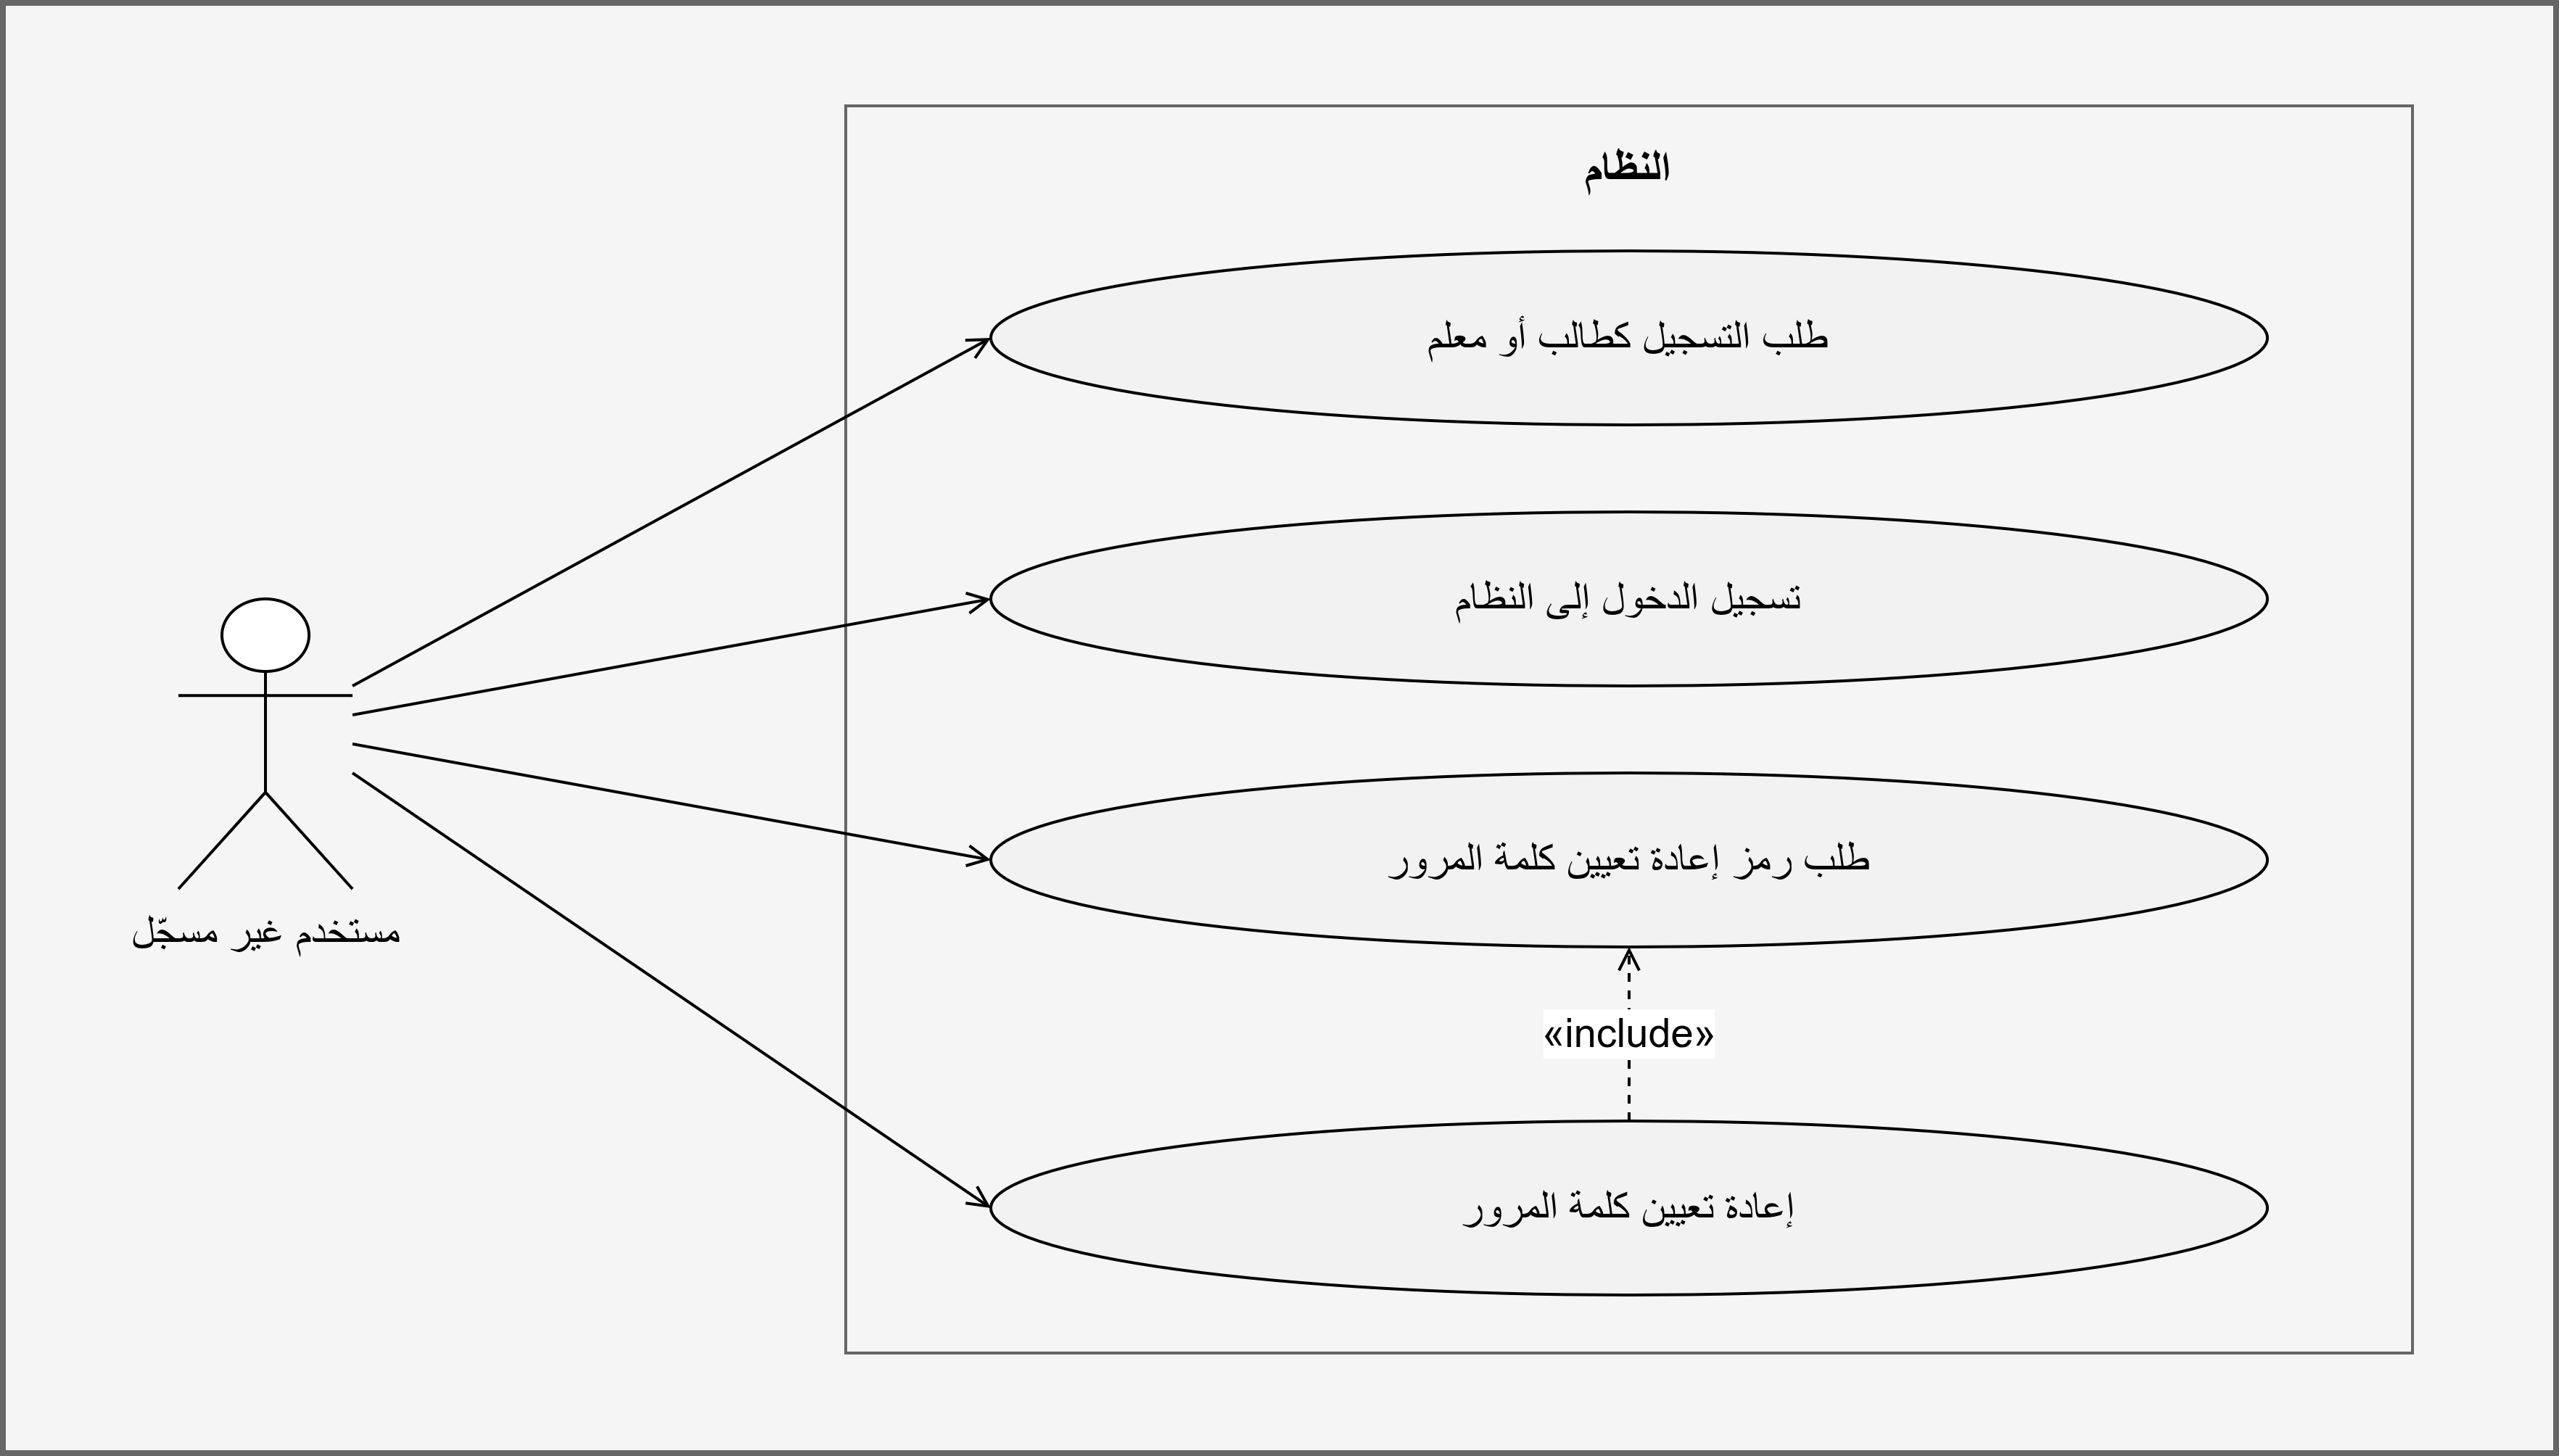
\includegraphics[width=\textwidth,height=0.8\textheight,keepaspectratio]{figures/uc-01-unregistered.png}
  \caption{حالات الاستخدام للمستخدم غير المسجّل: تبيّن ما يستطيع الزائر القيام به قبل امتلاك حساب، وهو محصور في التسجيل وتسجيل الدخول واستعادة كلمة المرور.}
  \label{fig:uc-01-unregistered}
\end{figure}

\clearpage
\subsection{حالات الاستخدام للمستخدمين المسجلين}

\begin{figure}[H]
  \centering
  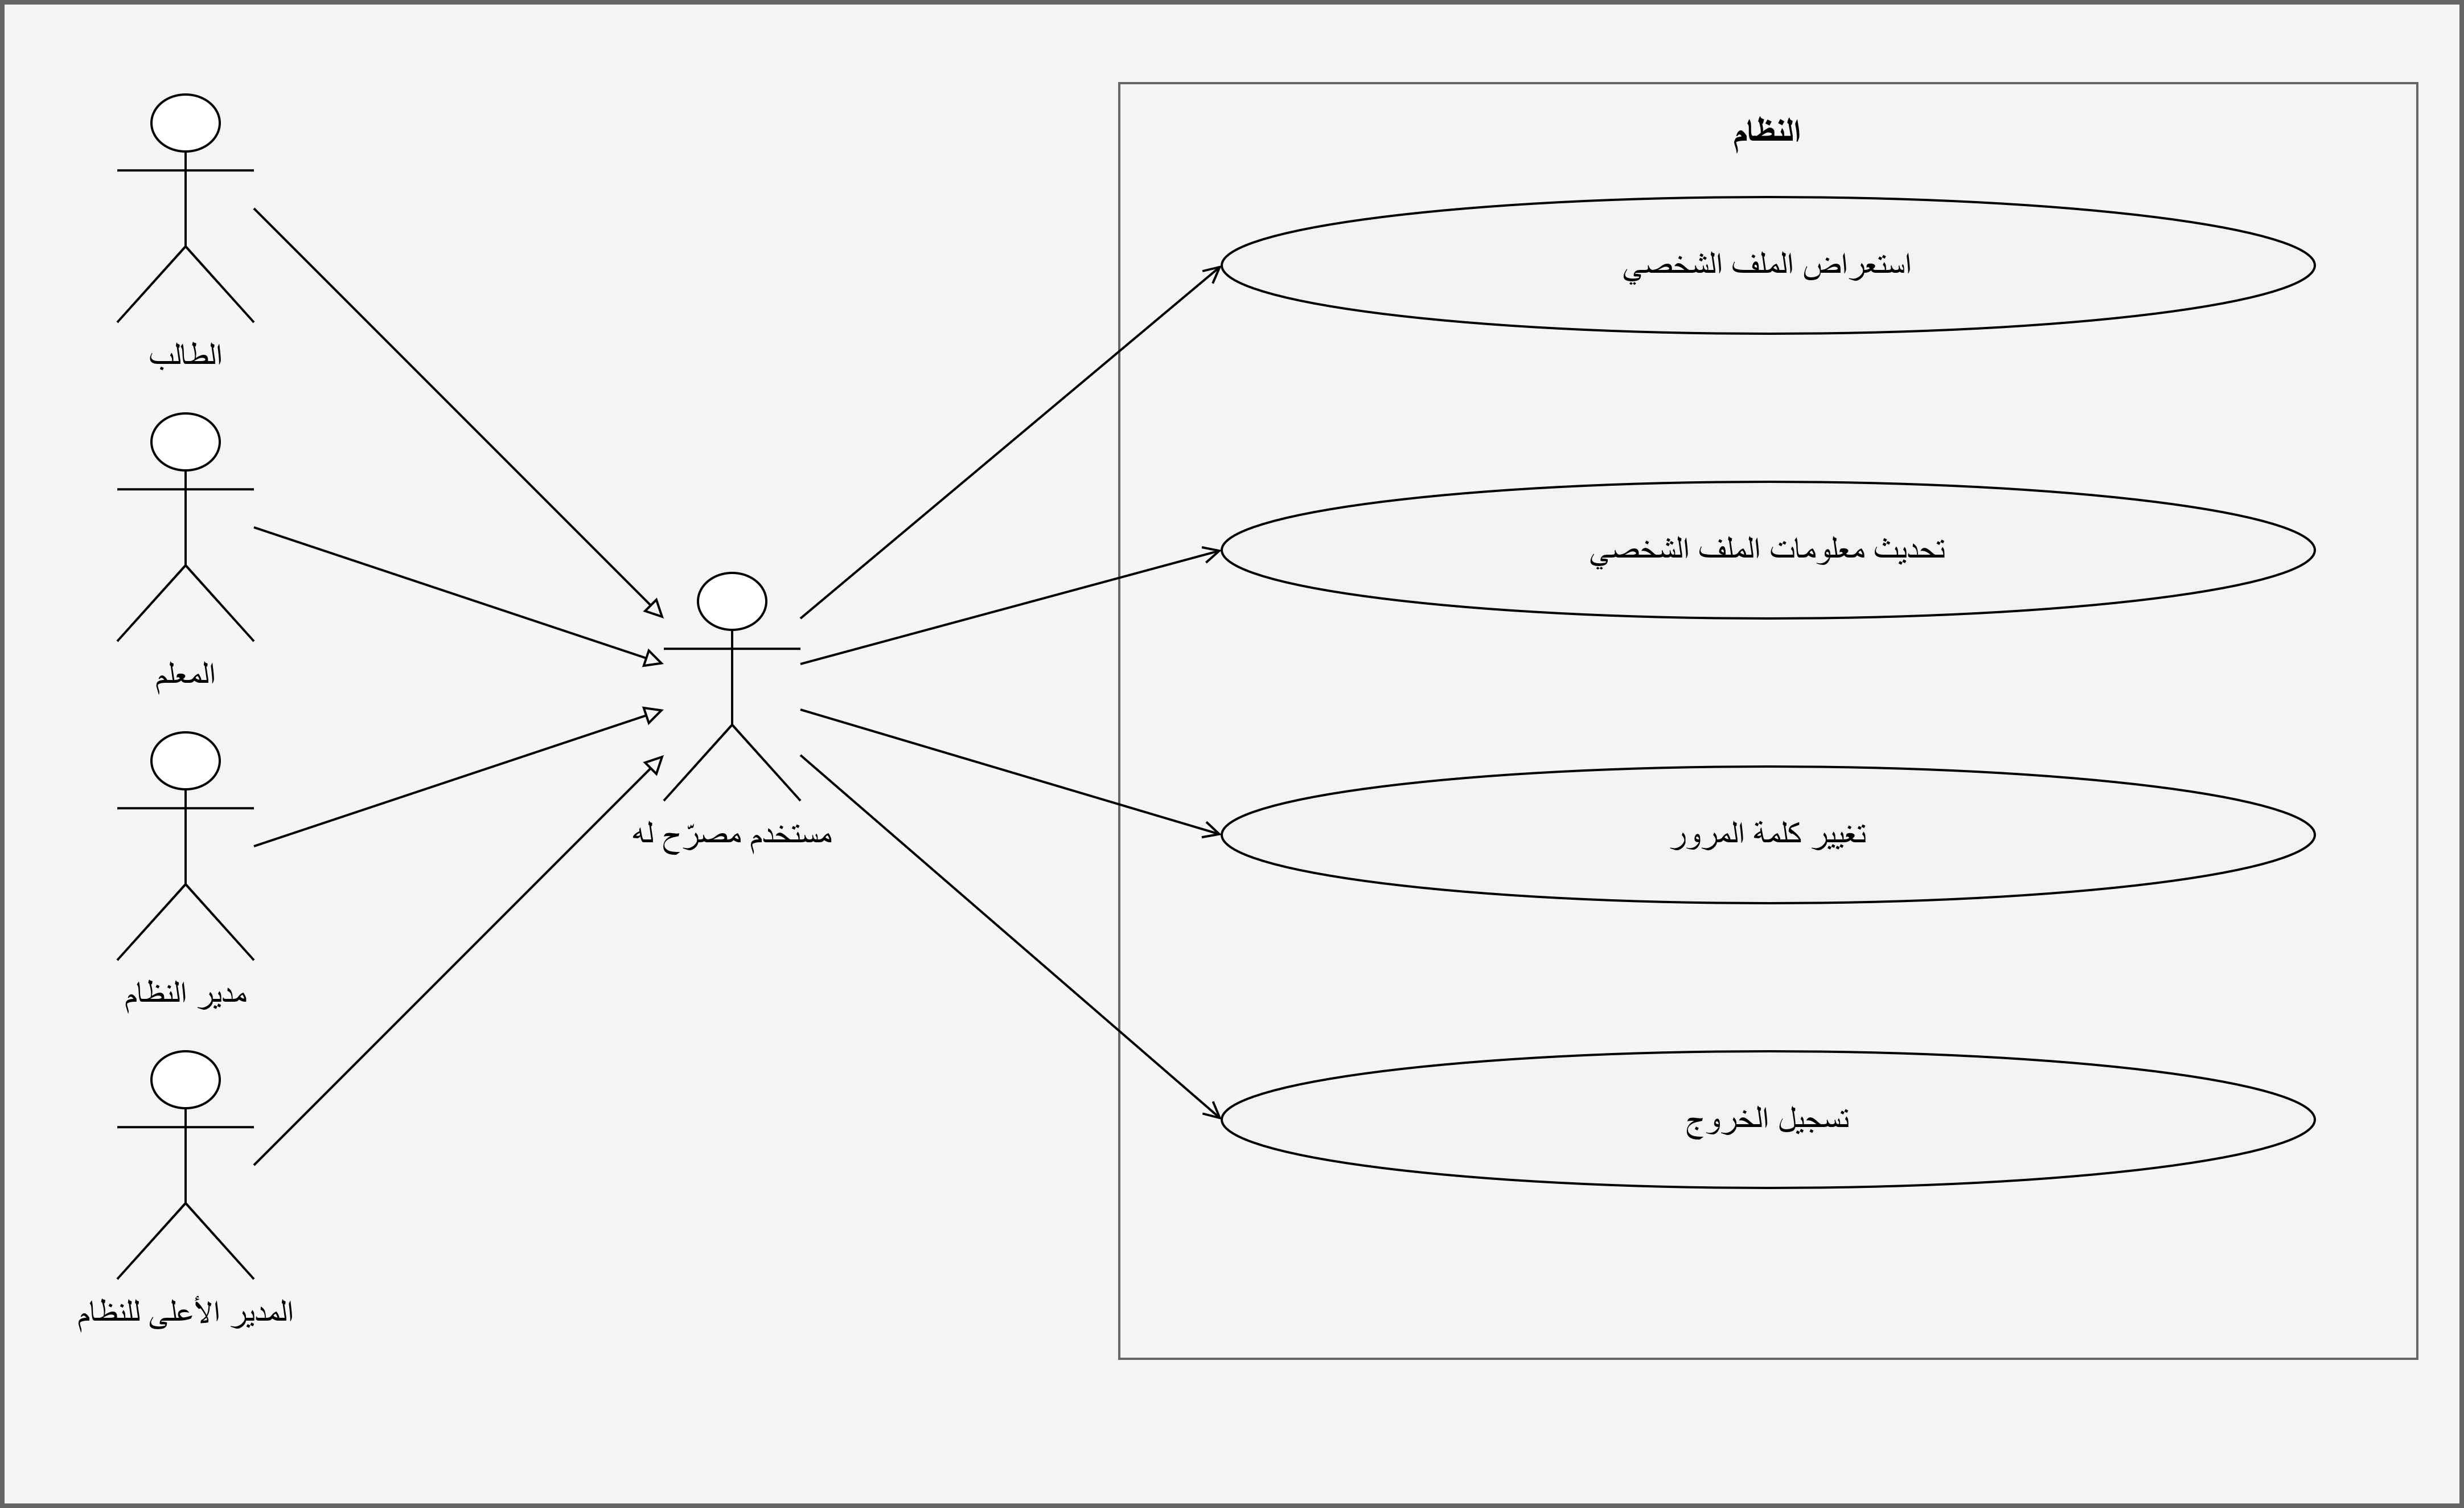
\includegraphics[width=\textwidth,height=0.8\textheight,keepaspectratio]{figures/uc-02-authorized.png}
  \caption{حالات الاستخدام المشتركة بين المستخدمين المسجّلين: العمليات المتاحة لكل صاحب حساب مهما كان دوره، وتتعلّق كلّها بإدارة ملفه الشخصي وجلسته.}
  \label{fig:uc-02-authorized}
\end{figure}

\clearpage
\subsection{حالات الاستخدام لمدير المظام الأعلى}

\begin{figure}[H]
  \centering
  \includegraphics[width=\textwidth,height=0.8\textheight,keepaspectratio]{figures/uc-03-super-admin.png}
  \caption{حالات الاستخدام لمدير النظام الأعلى: يتفرّد هذا الدور بإدارة حسابات المدراء وبالعمليات الهدّامة كحذف الفصول والجلسات ومخرجاتها.}
  \label{fig:uc-03-super-admin}
\end{figure}

\clearpage
\subsection{حالات الاستخدام لمدير النظام}

\begin{figure}[H]
  \centering
  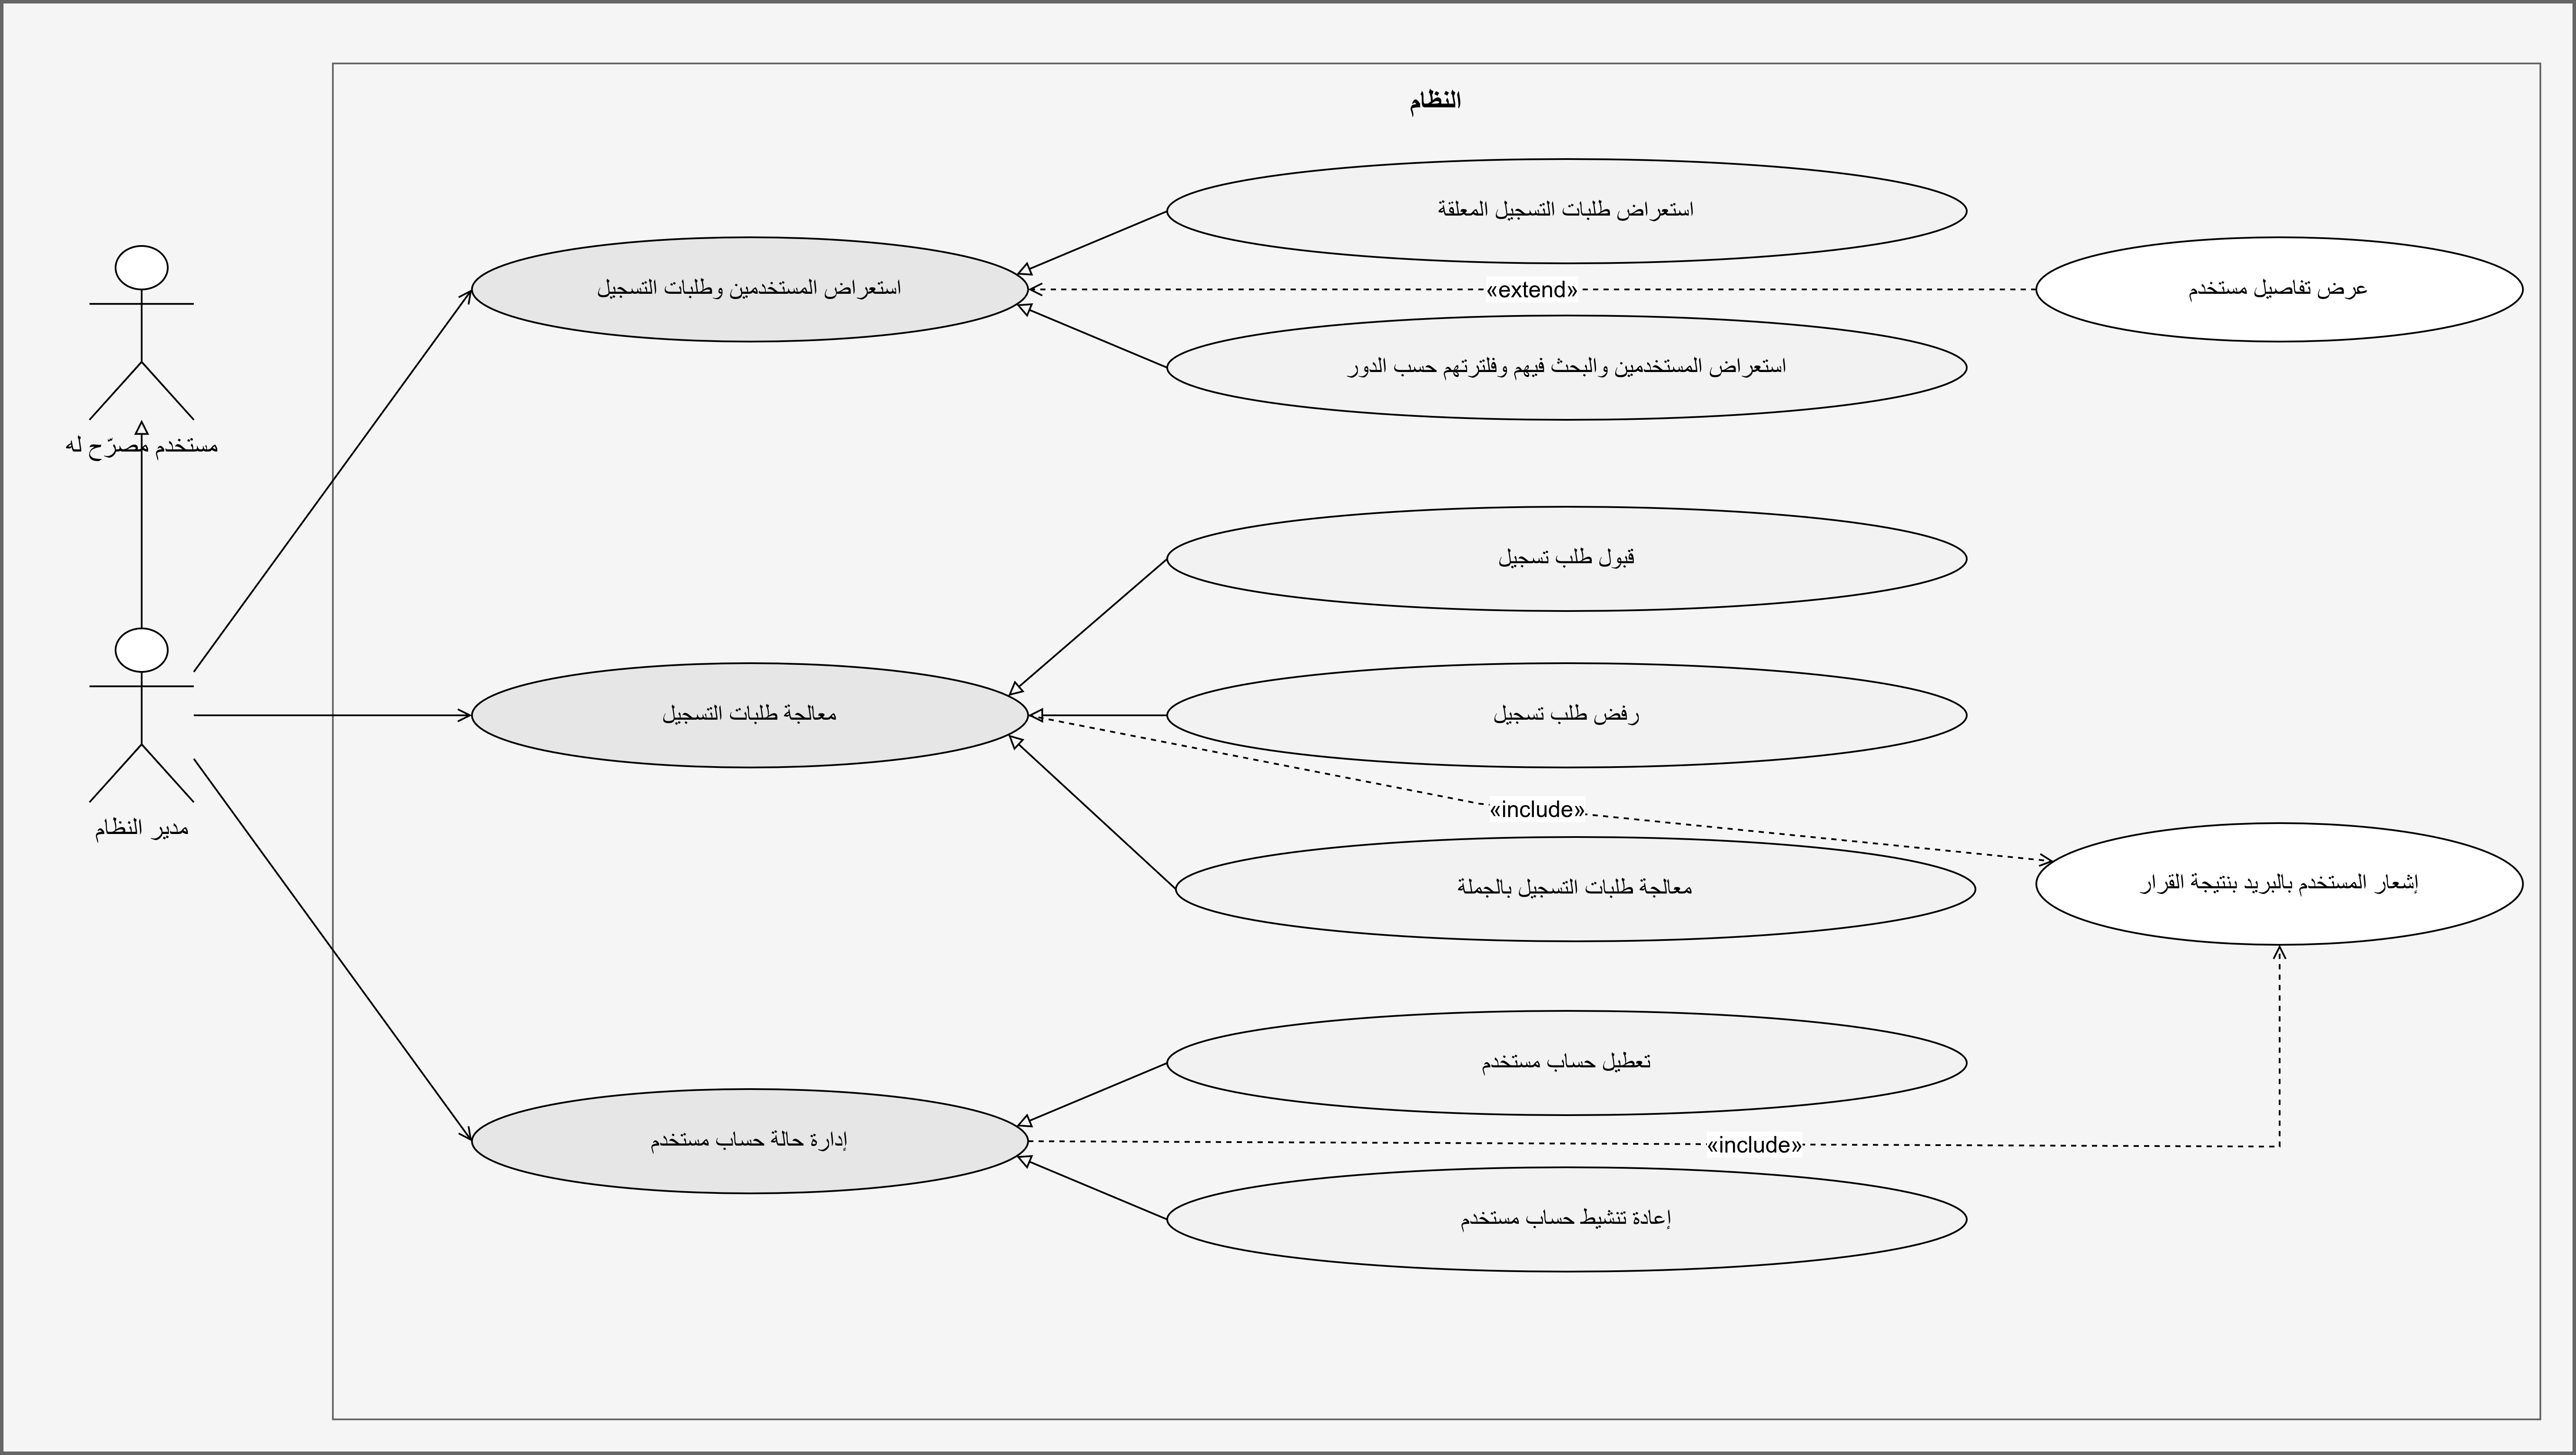
\includegraphics[width=\textwidth,height=0.8\textheight,keepaspectratio]{figures/uc-04-system-admin.png}
  \caption{حالات الاستخدام لمدير النظام: تتمحور حول معالجة طلبات التسجيل وإدارة حالات حسابات المستخدمين، دون صلاحية على حسابات المدراء أنفسهم.}
  \label{fig:uc-04-system-admin}
\end{figure}

\clearpage
\subsection{حالات الاستخدام للمعلم}

\begin{figure}[H]
  \centering
  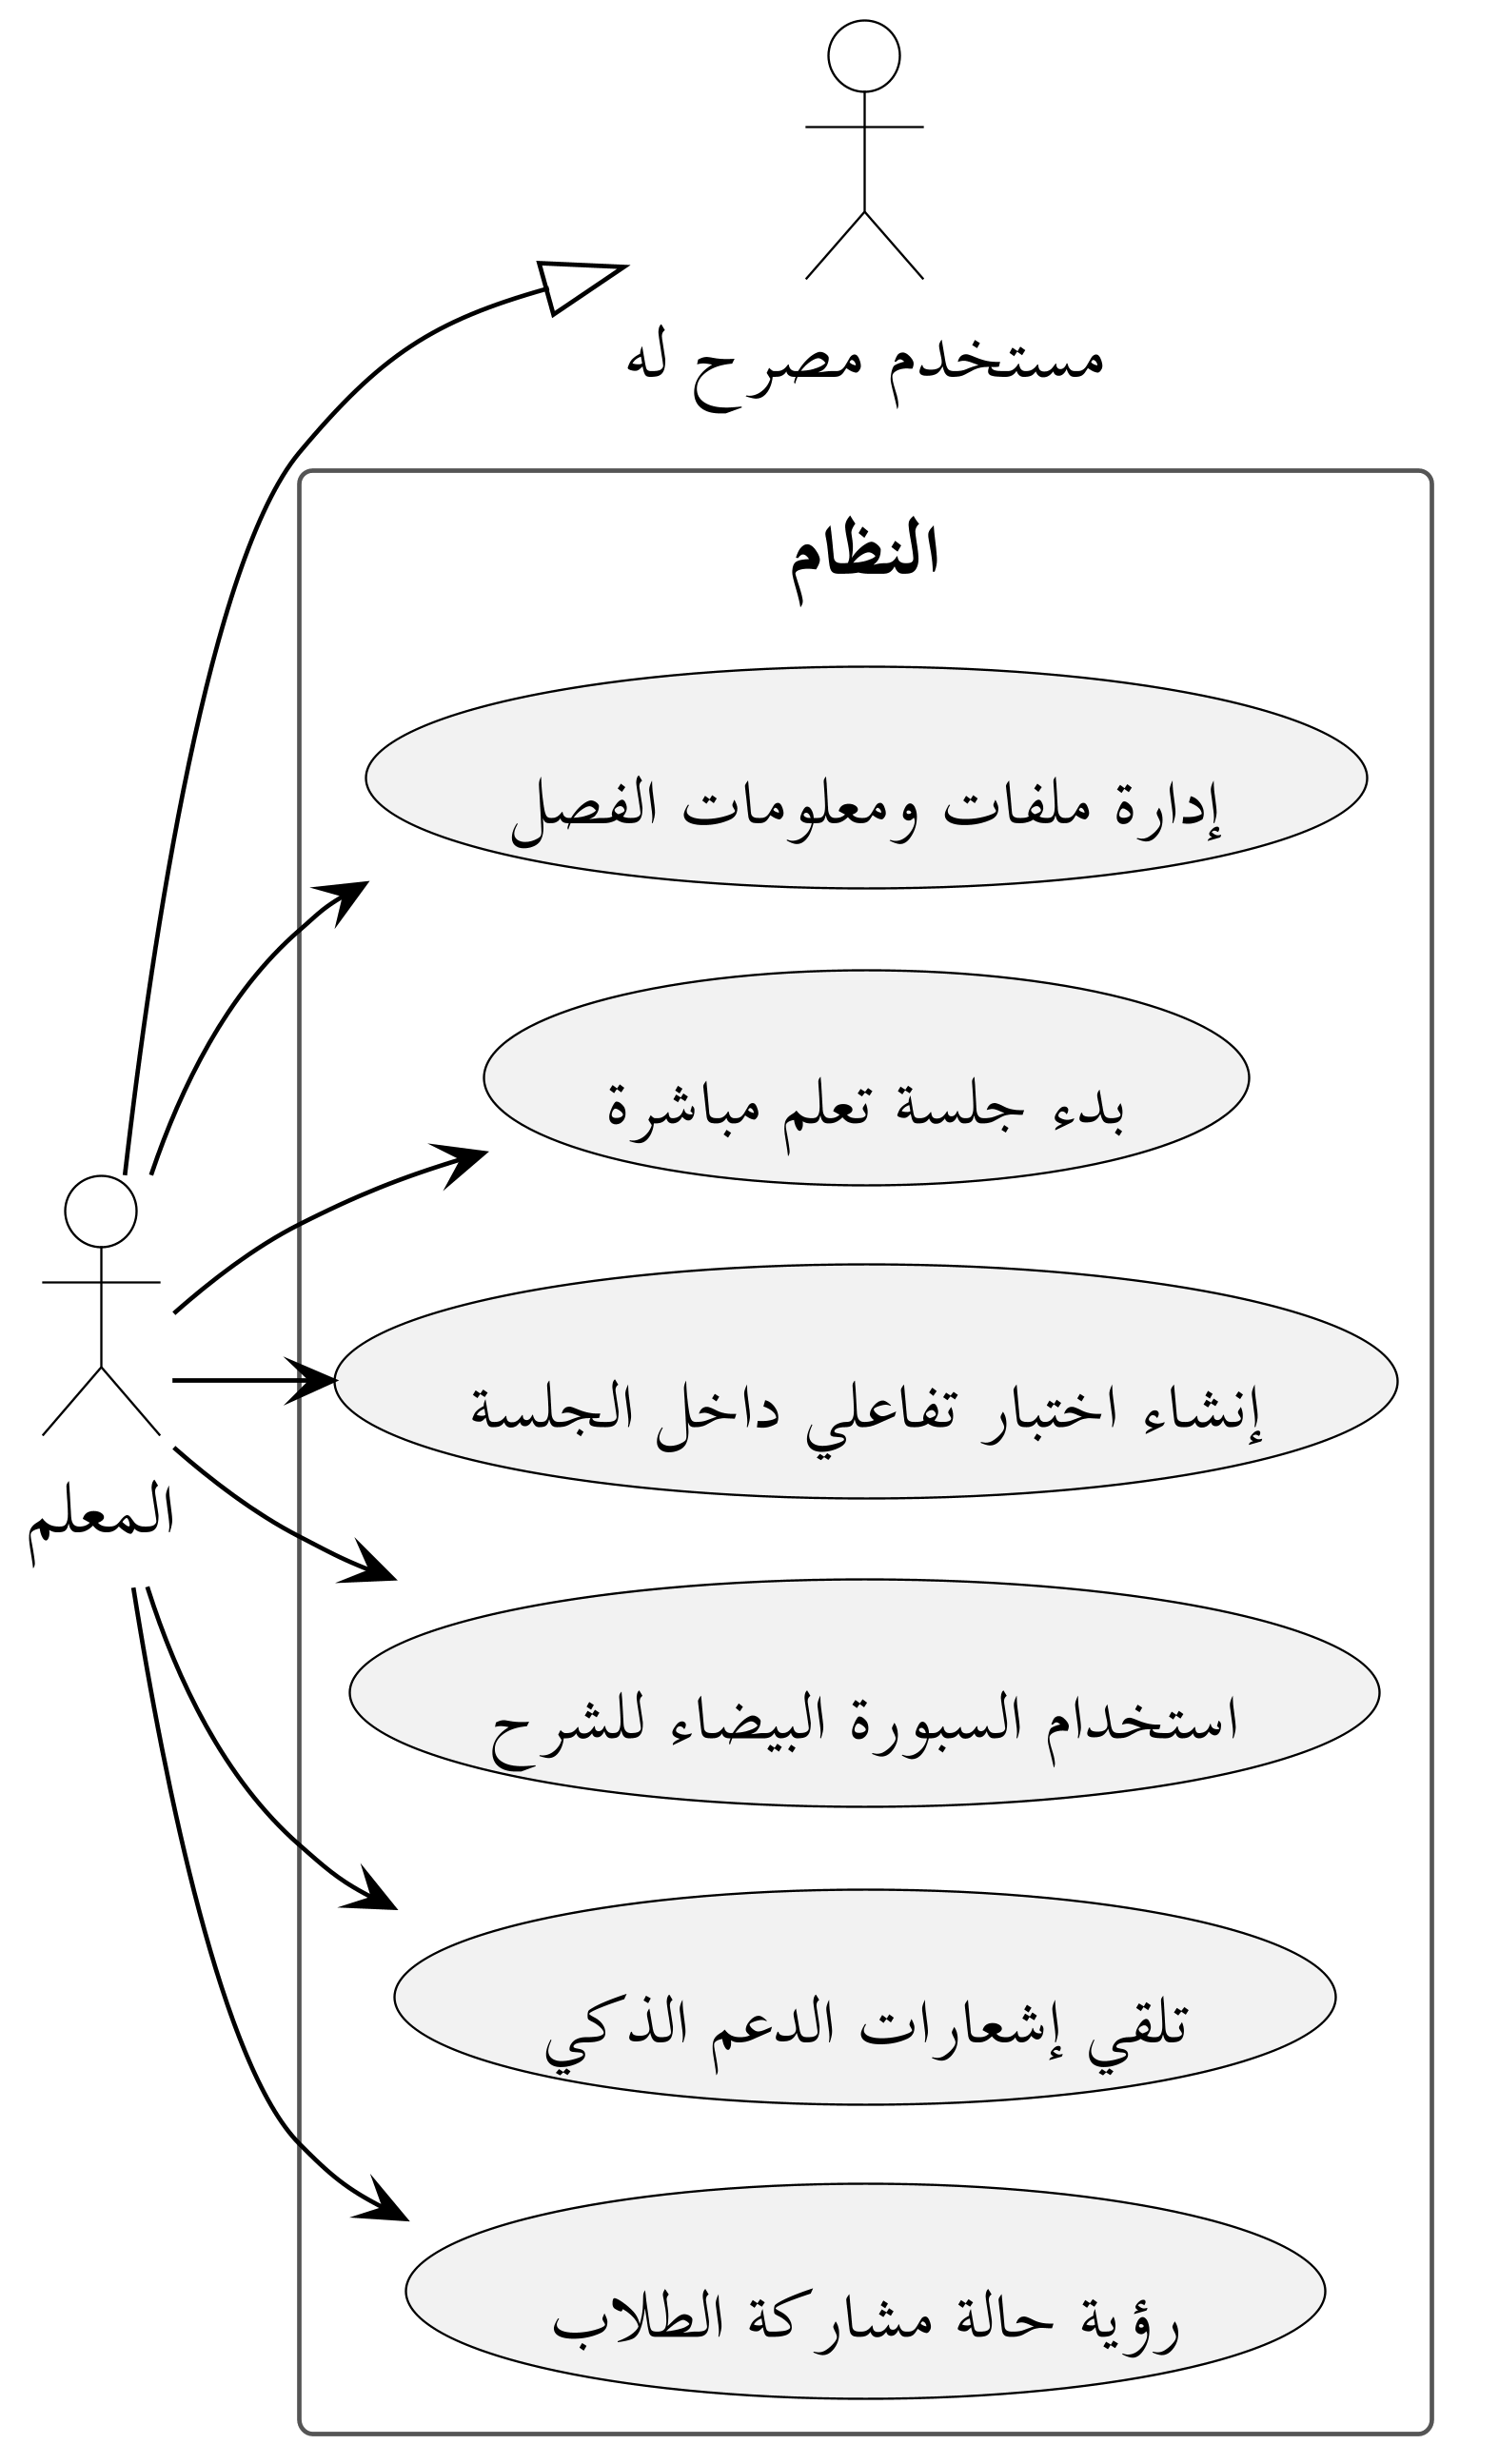
\includegraphics[width=\textwidth,height=0.8\textheight,keepaspectratio]{figures/uc-05-teacher.png}
  \caption{حالات الاستخدام للمعلم: تشمل إدارة فصوله وموادّه المرجعية، وإدارة دورة حياة الجلسة المباشرة من بدئها حتى إنهائها والاطّلاع على مخرجاتها.}
  \label{fig:uc-05-teacher}
\end{figure}

\clearpage
\subsection{حالات الاستخدام للطالب}

\begin{figure}[H]
  \centering
  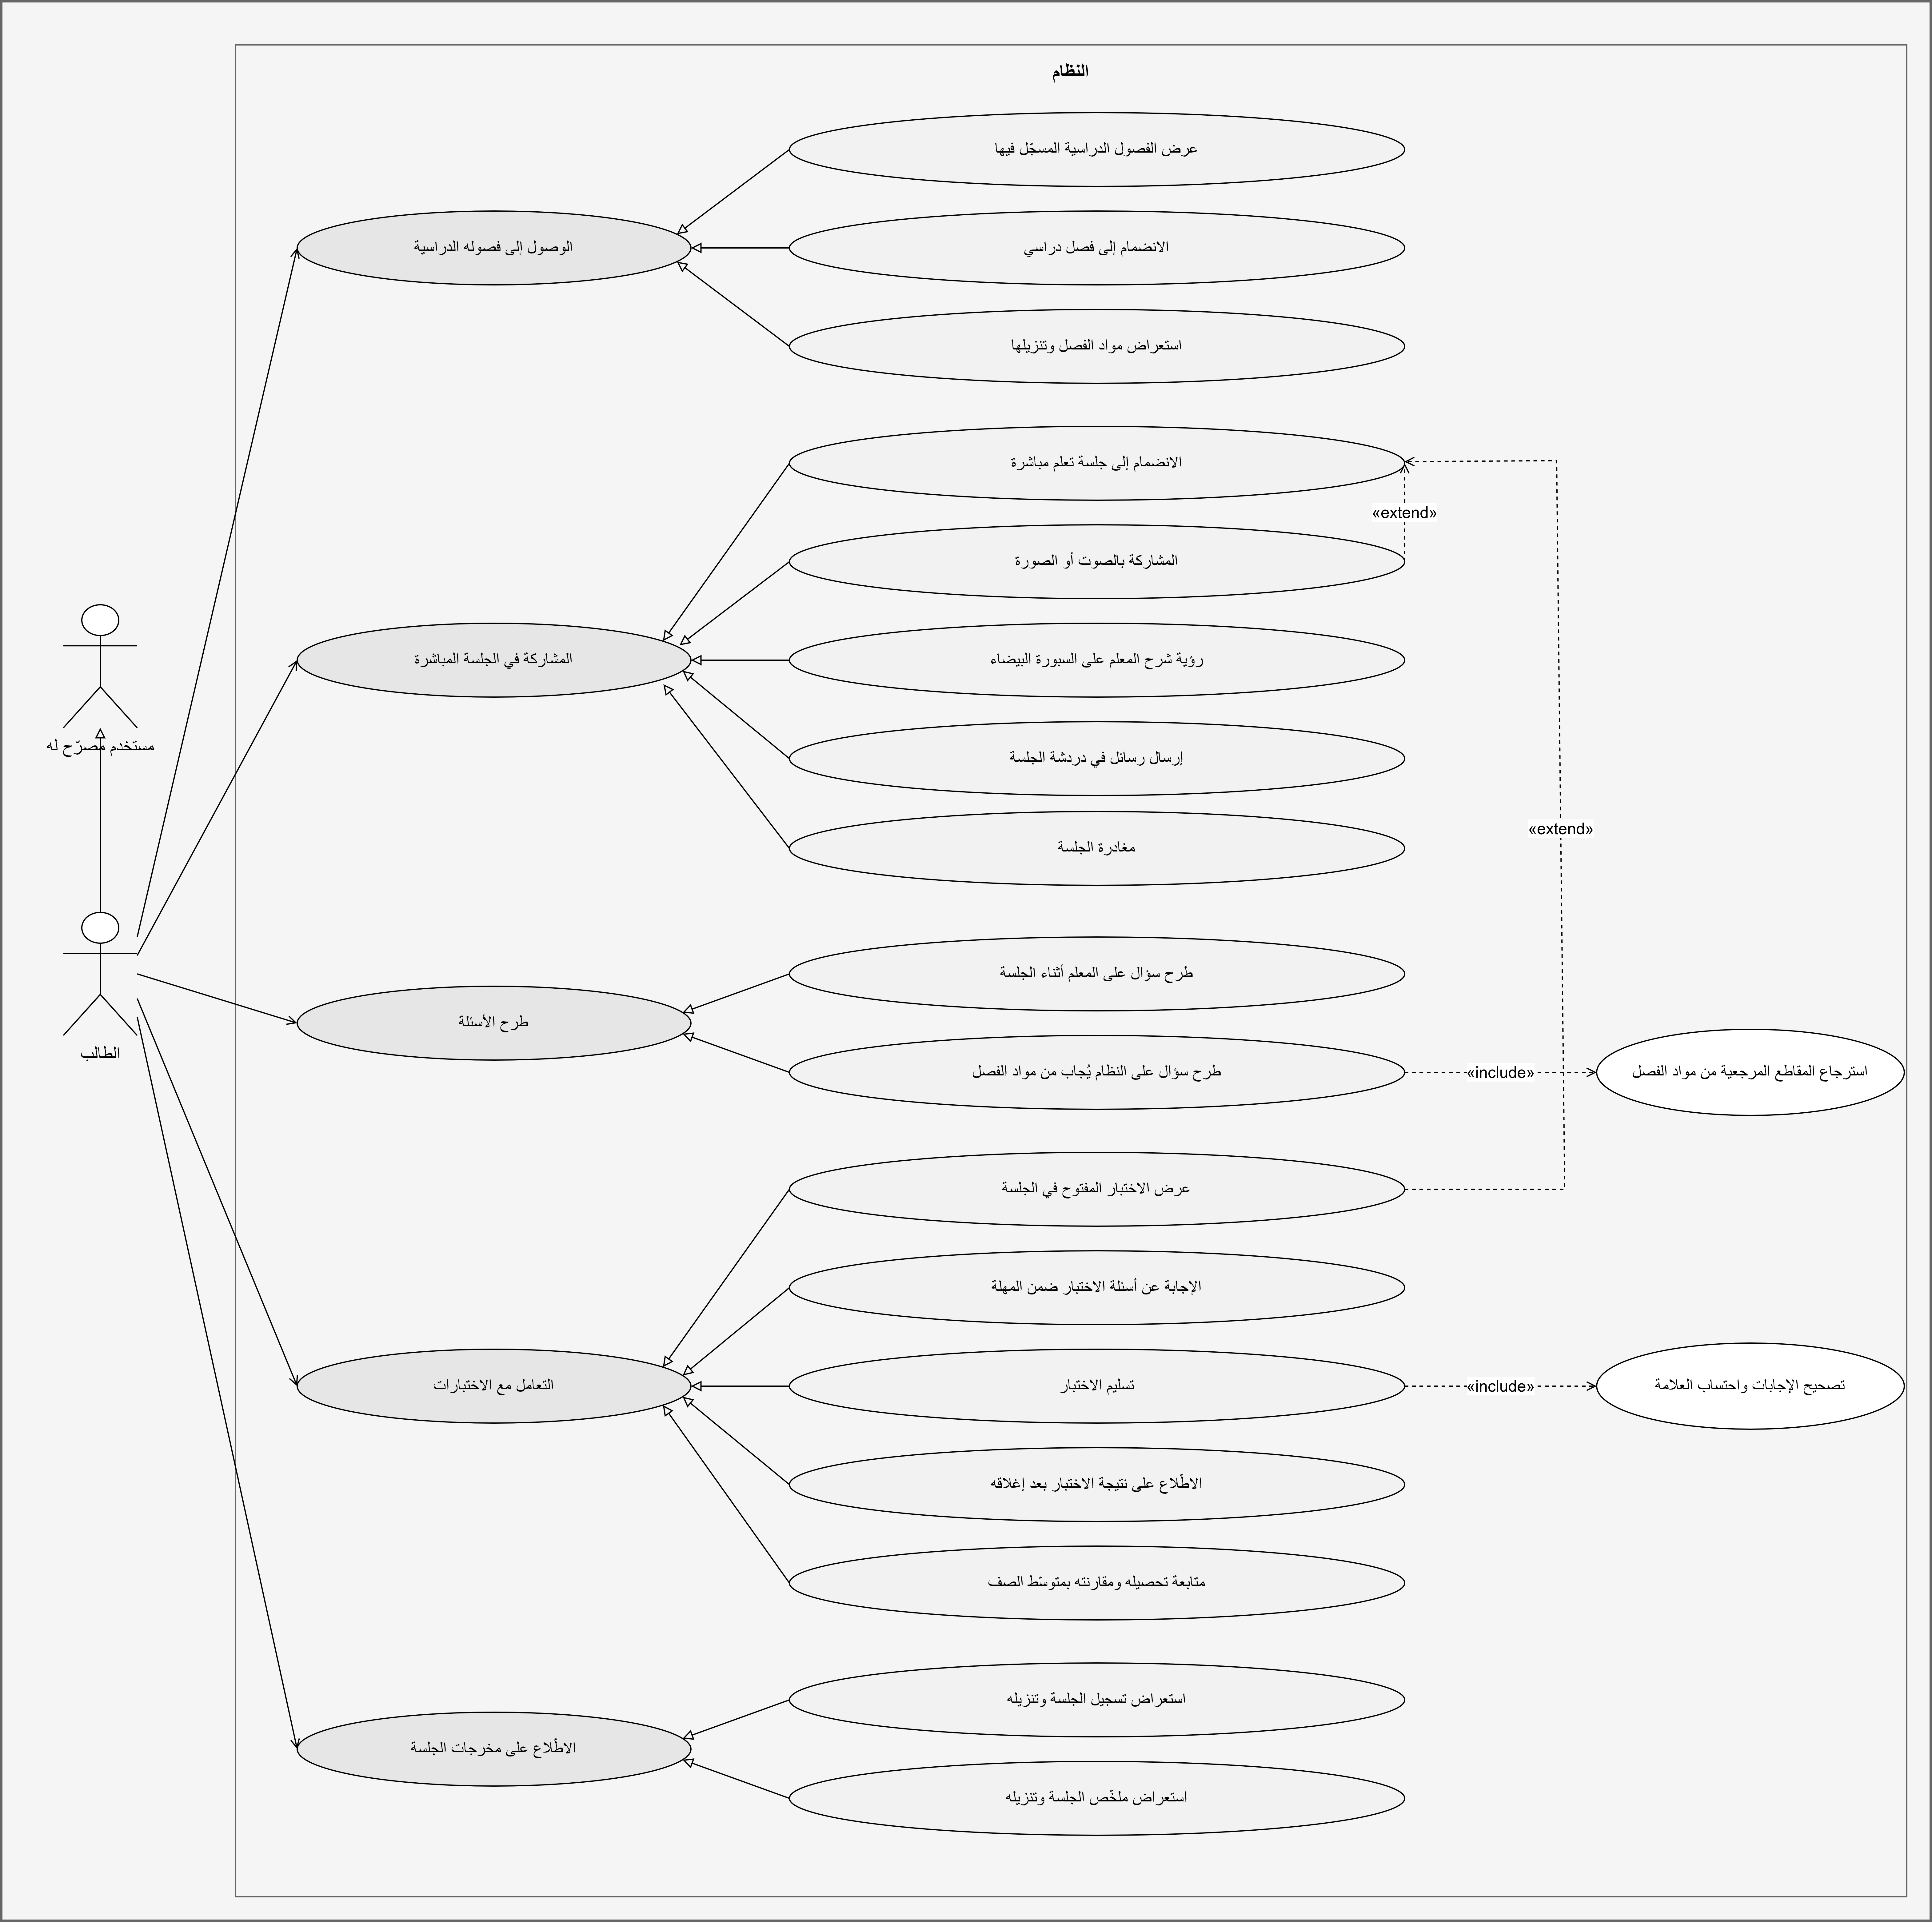
\includegraphics[width=\textwidth,height=0.8\textheight,keepaspectratio]{figures/uc-06-student.png}
  \caption{حالات الاستخدام للطالب: الانضمام إلى الجلسات المباشرة والتفاعل داخلها وطرح الأسئلة على النظام والاطّلاع على مخرجات الجلسة بعد انتهائها.}
  \label{fig:uc-06-student}
\end{figure}

\clearpage
\section{السرد النصي لحالات الاستخدام}

% ===========================================================================
% NARRATIVE SET — 7 use cases, ordered by system lifecycle, not by actor.
% Each narrative's preconditions are the previous one's postconditions.
% Fill them one at a time; find the empty ones with:
%   grep -n "TODO(uc-" chapters/04-requirements-analysis.tex
% Section 3 (SSDs) must mirror these seven in the same order.
% ===========================================================================

\subsection{تحضير المادة المرجعية}

\subsubsection{السرد النصي لحالة رفع ملف مرجعي إلى الفصل وفهرسته}
\label{subsubsec:uc-ingest}

\begin{enumerate}
  \item الاسم: رفع ملف مرجعي إلى الفصل الدراسي وفهرسته في قاعدة المعرفة
  \item الفاعل: المعلم
  \item الوصف: يرفع المعلم ملفًّا إلى فصله الدراسي، فيحفظه النظام ويعالج محتواه ويهيّئه للاسترجاع، حتى تصبح المادة مرجعًا يعتمد عليه في مساعدة المعلم وفي الإجابة عن أسئلة الطلاب.
  \item الشروط المسبقة
  \begin{enumerate}
    \item أن يكون المعلم مسجّلًا دخوله وأن يكون معلّم الفصل الدراسي المقصود.
    \item أن يكون الفصل الدراسي موجودًا.
  \end{enumerate}
  \item الشروط اللاحقة
  \begin{enumerate}
    \item أن يُحفظ الملف وأن تُسجَّل بياناته ضمن ملفات الفصل الدراسي.
    \item تصبح حالة فهرسة الملف ظاهرة للمعلم.
    \item أن يصبح محتوى الملف متاحًا للاسترجاع عند اكتمال الفهرسة بنجاح.
  \end{enumerate}
  \item السيناريو الرئيسي (المسار الناجح)
\end{enumerate}

\begin{ucflow}{السرد النصي لحالة الاستخدام «رفع ملف مرجعي إلى الفصل وفهرسته»: يعرض خطوات المسار الرئيسي مقابلةً بين ما يقوم به الفاعل وما يستجيب به النظام في كل خطوة.}{المعلم}
    1. يطلب المعلم رفع ملفات لفصله الدراسي. &  \\ \hline
     & 2. يعرض النظام حدود الرفع من حجم أقصى وصيغ مقبولة، قبل أن يختار المعلم ملفًّا. \\ \hline
    3. يختار المعلم الملف ويؤكّد رفعه. &  \\ \hline
     & 4. يتحقّق النظام من هوية الفاعل ومن كونه معلّم هذا الفصل. \\ \hline
     & 5. يتحقّق النظام من أنّ الملف غير فارغ وأنّ حجمه ضمن الحدّ الأقصى، ومن أنّ صيغته مقبولة اعتمادًا على نوع محتواه أو امتداده. \\ \hline
     & 6. يحفظ النظام الملف ضمن الفصل الدراسي بمعرّف فريد يمنع تضارب الأسماء المتشابهة. \\ \hline
     & 7. يسجّل النظام بيانات الملف من اسم ونوع وحجم ضمن ملفات الفصل. \\ \hline
     & 8. يُعلم النظام المعلم بنجاح الرفع ويُظهر الملف في قائمة ملفات الفصل مبيّنًا حالة فهرسته. \\ \hline
     & 9. يستخرج النظام نصّ الملف بحسب صيغته، ويستخرجه كذلك من صفحاته المصوَّرة التي لا نصّ فيها. \\ \hline
     & 10. يقسّم النظام النصّ المستخرج إلى مقاطع ويهيّئها للاسترجاع، فتصبح حالة الملف «مفهرَس». \\ \hline
\end{ucflow}

\begin{enumerate}
  \item المسارات البديلة (الاستثناءات)
  \begin{enumerate}
    \item \textbf{4: اذا كان الفاعل ليس معلّم الفصل يرفض النظام الطلب. }
    \item \textbf{5: اذا كان حجم الملف يتجاوز الحدّ الأقصى يرفض النظام الطلب. }
    \item \textbf{5: اذا كان الملف فارغًا يرفض النظام الرفع ويُعلم المعلم بالحدّ المسموح. }
    \item \textbf{5: اذا كانت صيغة الملف غير مقبولة يرفض النظام الرفع ويعرض للمعلم الصيغ المقبولة. }
    \item \textbf{9: اذا كان محتوى الملف مطابقًا لآخر فهرسة ناجحة تُعدّ الفهرسة مكتملة من غير إعادة معالجته، لأنّ ما فُهرس منه سابقًا ما يزال صالحًا. }
    \item \textbf{9: اذا لم يُستخرج من الملف أيّ نصّ يُعلم النظام المعلم بتعذّر فهرسته مع بيان السبب، ولا يَعُدّه مفهرسًا. }
    \item \textbf{10: اذا تعذّرت فهرسة الملف يبقى رفعه ناجحًا، ويبقى الملف غير مفهرس إلى أن تطلب إعاد الفهرسة يدويًّا. }
  \end{enumerate}
\end{enumerate}

\subsection{جلسة التعلم المباشرة}

\subsubsection{السرد النصي لحالة الشرح على السبورة والتفاعل داخل الجلسة}
\label{subsubsec:uc-whiteboard}

\begin{enumerate}
  \item الاسم: الشرح على السبورة البيضاء والتفاعل داخل جلسة التعلم المباشرة
  \item الفاعل: المعلم فاعلًا رئيسًا، والطالب فاعلًا مشاركًا
  \item الوصف: يشرح المعلم على سبورة بيضاء تعلو صورة الجلسة، فيرى الطلاب ما يرسمه المعلم، ويتفاعلون معه في أثناء ذلك بالدردشة وبطرح الأسئلة، ويضبط المعلم ما يُسمح لهم بمشاركته من صوت أو صورة.
  \item الشروط المسبقة
  \begin{enumerate}
    \item أن تكون جلسة التعلم المباشرة جارية وأن يكون المعلم متّصلًا بها.
    \item أن يكون الطلاب المشاركون أعضاء في الفصل الدراسي وقد انضمّوا إلى الجلسة.
  \end{enumerate}
  \item الشروط اللاحقة
  \begin{enumerate}
    \item أن يرى المشاركون جميعًا السبورة نفسها بما عليها.
    \item أن تُحفظ رسائل الدردشة وأسئلة الجلسة وإجاباتها ضمن سجل الجلسة.
    \item أن يسري ما قرّره المعلم في مشاركة الطلاب للصوت والصورة على الجلسة كلّها.
  \end{enumerate}
  \item السيناريو الرئيسي (المسار الناجح)
\end{enumerate}

\begin{ucflow}{السرد النصي لحالة الاستخدام «الشرح على السبورة والتفاعل داخل الجلسة»: يعرض خطوات المسار  أوّلًا بأوّلالرئيسي مقابلةً بين ما يقوم به الفاعل وما يستجيب به النظام في كل خطوة.}{المعلم والطالب}
    1. يُفعّل المعلم السبورة البيضاء، مختارًا الرسم فوق ما يعرضه على الطلاب أو على سطح فارغ. &  \\ \hline
     & 2. يعرض النظام سطح الرسم مضبوطًا على أبعاد الصورة المعروضة، ويتيح للمعلم أدوات القلم والأشكال والنص والمؤشّر الضوئي والممحاة. \\ \hline
    3. يرسم المعلم على السبورة أو يكتب عليها في أثناء شرحه. &  \\ \hline
     & 4. يُظهر النظام ما يرسمه المعلم على شاشات الطلاب، في موضعه نفسه من الصورة مهما اختلفت أحجام شاشاتهم. \\ \hline
    5. يجمّد المعلم الصورة ليشرح على لقطة بعينها، ثمّ يرفع التجميد. &  \\ \hline
     & 6. يثبّت النظام اللقطة نفسها عند الطلاب جميعًا، ثمّ يعيدهم إلى البثّ المباشر عند رفع التجميد. \\ \hline
     & 7. يزوّد النظام كلّ طالب ينضم بعد بدء الشرح بما رُسم على السبورة قبل انضمامه، فيرى ما يراه بقيّة الصف. \\ \hline
    8. يتراجع المعلم عن آخر ما رسمه، أو يخفي السبورة، أو يمسحها كلّها. &  \\ \hline
     & 9. يحدّث النظام السبورة عند المشاركين جميعًا بحيث تبقى واحدة عندهم. \\ \hline
    10. يرسل أحد المشاركين رسالة في دردشة الجلسة. &  \\ \hline
     & 11. يوزّع النظام الرسالة على المشاركين في الجلسة ويحفظها في سجل دردشتها. \\ \hline
    12. يطرح الطالب سؤالًا على المعلم في أثناء الشرح. &  \\ \hline
     & 13. يعرض النظام السؤال للمعلم ضمن أسئلة الجلسة. \\ \hline
    14. يجيب المعلم عن السؤال. &  \\ \hline
     & 15. يعرض النظام الإجابة مقترنة بسؤالها للمشاركين. \\ \hline
    16. يسمح المعلم للطلاب بمشاركة الصوت أو الصورة، أو يمنعهم منها. &  \\ \hline
     & 17. يطبّق النظام قرار المعلم على الجلسة ويُعلم المشاركين جميعًا بما صار مسموحًا لهم. \\ \hline
\end{ucflow}

\begin{enumerate}
  \item المسارات البديلة (الاستثناءات)
  \begin{enumerate}
    \item \textbf{2: اذا كان الفاعل ليس معلّم الجلسة لا يتيح له النظام الرسم على السبورة، ويكتفي بعرضها عليه. }
    \item \textbf{4: اذا انقطع اتّصال طالب في أثناء الرسم يستدرك النظام ما فاته عند عودته، فتعود سبورته مطابقة لسبورة المعلم. }
    \item \textbf{4: اذا تعذّر إيصال ما رُسم لحظتَه لا يقطع النظام الشرح، وتُصحَّح السبورة في أوّل مزامنة تالية. }
    \item \textbf{7: اذا كان المعلم هو من أُعيد اتّصاله بالجلسة يعيد النظام مزامنة السبورة عند المشاركين جميعًا، حتى لا تبقى عندهم رسوم لم يعد المعلم قادرًا على محوها. }
    \item \textbf{11: اذا كانت الرسالة فارغة يهملها النظام ولا يوزّعها. }
    \item \textbf{16: اذا كان الفاعل ليس معلّم الجلسة يرفض النظام تغيير ما يُسمح به للطلاب. }
    \item \textbf{17: اذا منع المعلم مشاركة الصوت أو الصورة يوقف النظام ما هو منشور منهما ويمنع أيّ مشاركة جديدة إلى أن يُعاد السماح.}
  \end{enumerate}
\end{enumerate}

\subsubsection{السرد النصي لحالة تحليل شرح المعلم وإشعار المساعد المباشر}
\label{subsubsec:uc-drift}
% TODO(uc-3)

\subsubsection{السرد النصي لحالة طرح سؤال يُجاب من مواد الفصل}
\label{subsubsec:uc-qa}
% TODO(uc-4)

\subsection{الاختبارات داخل الجلسة}

\subsubsection{السرد النصي لحالة إنشاء مسودة اختبار وتعديلها ونشرها}
\label{subsubsec:uc-quiz-compose}
% TODO(uc-5)

\subsubsection{السرد النصي لحالة الإجابة عن الاختبار وتسليمه وتصحيحه}
\label{subsubsec:uc-quiz-answer}
% TODO(uc-6)

\subsection{مخرجات الجلسة}

\subsubsection{السرد النصي لحالة إنهاء الجلسة وتوليد الملخّص}
\label{subsubsec:uc-session-end}
% TODO(uc-7)

\section{مخططات تسلسل النظام}

\subsection{مخطط تسلسل النظام لحالات استخدام مدير النظام الاعلى}

\subsubsection{تدفّق تسجيل دخول المدير الأعلى}
\label{subsubsec:flow-super-admin-login}

يجري تسجيل دخول المدير الأعلى على مرحلتين يبيّنهما الشكلان~\ref{fig:flow-01a} و\ref{fig:flow-01b}.

\begin{figure}[htbp]
  \centering
  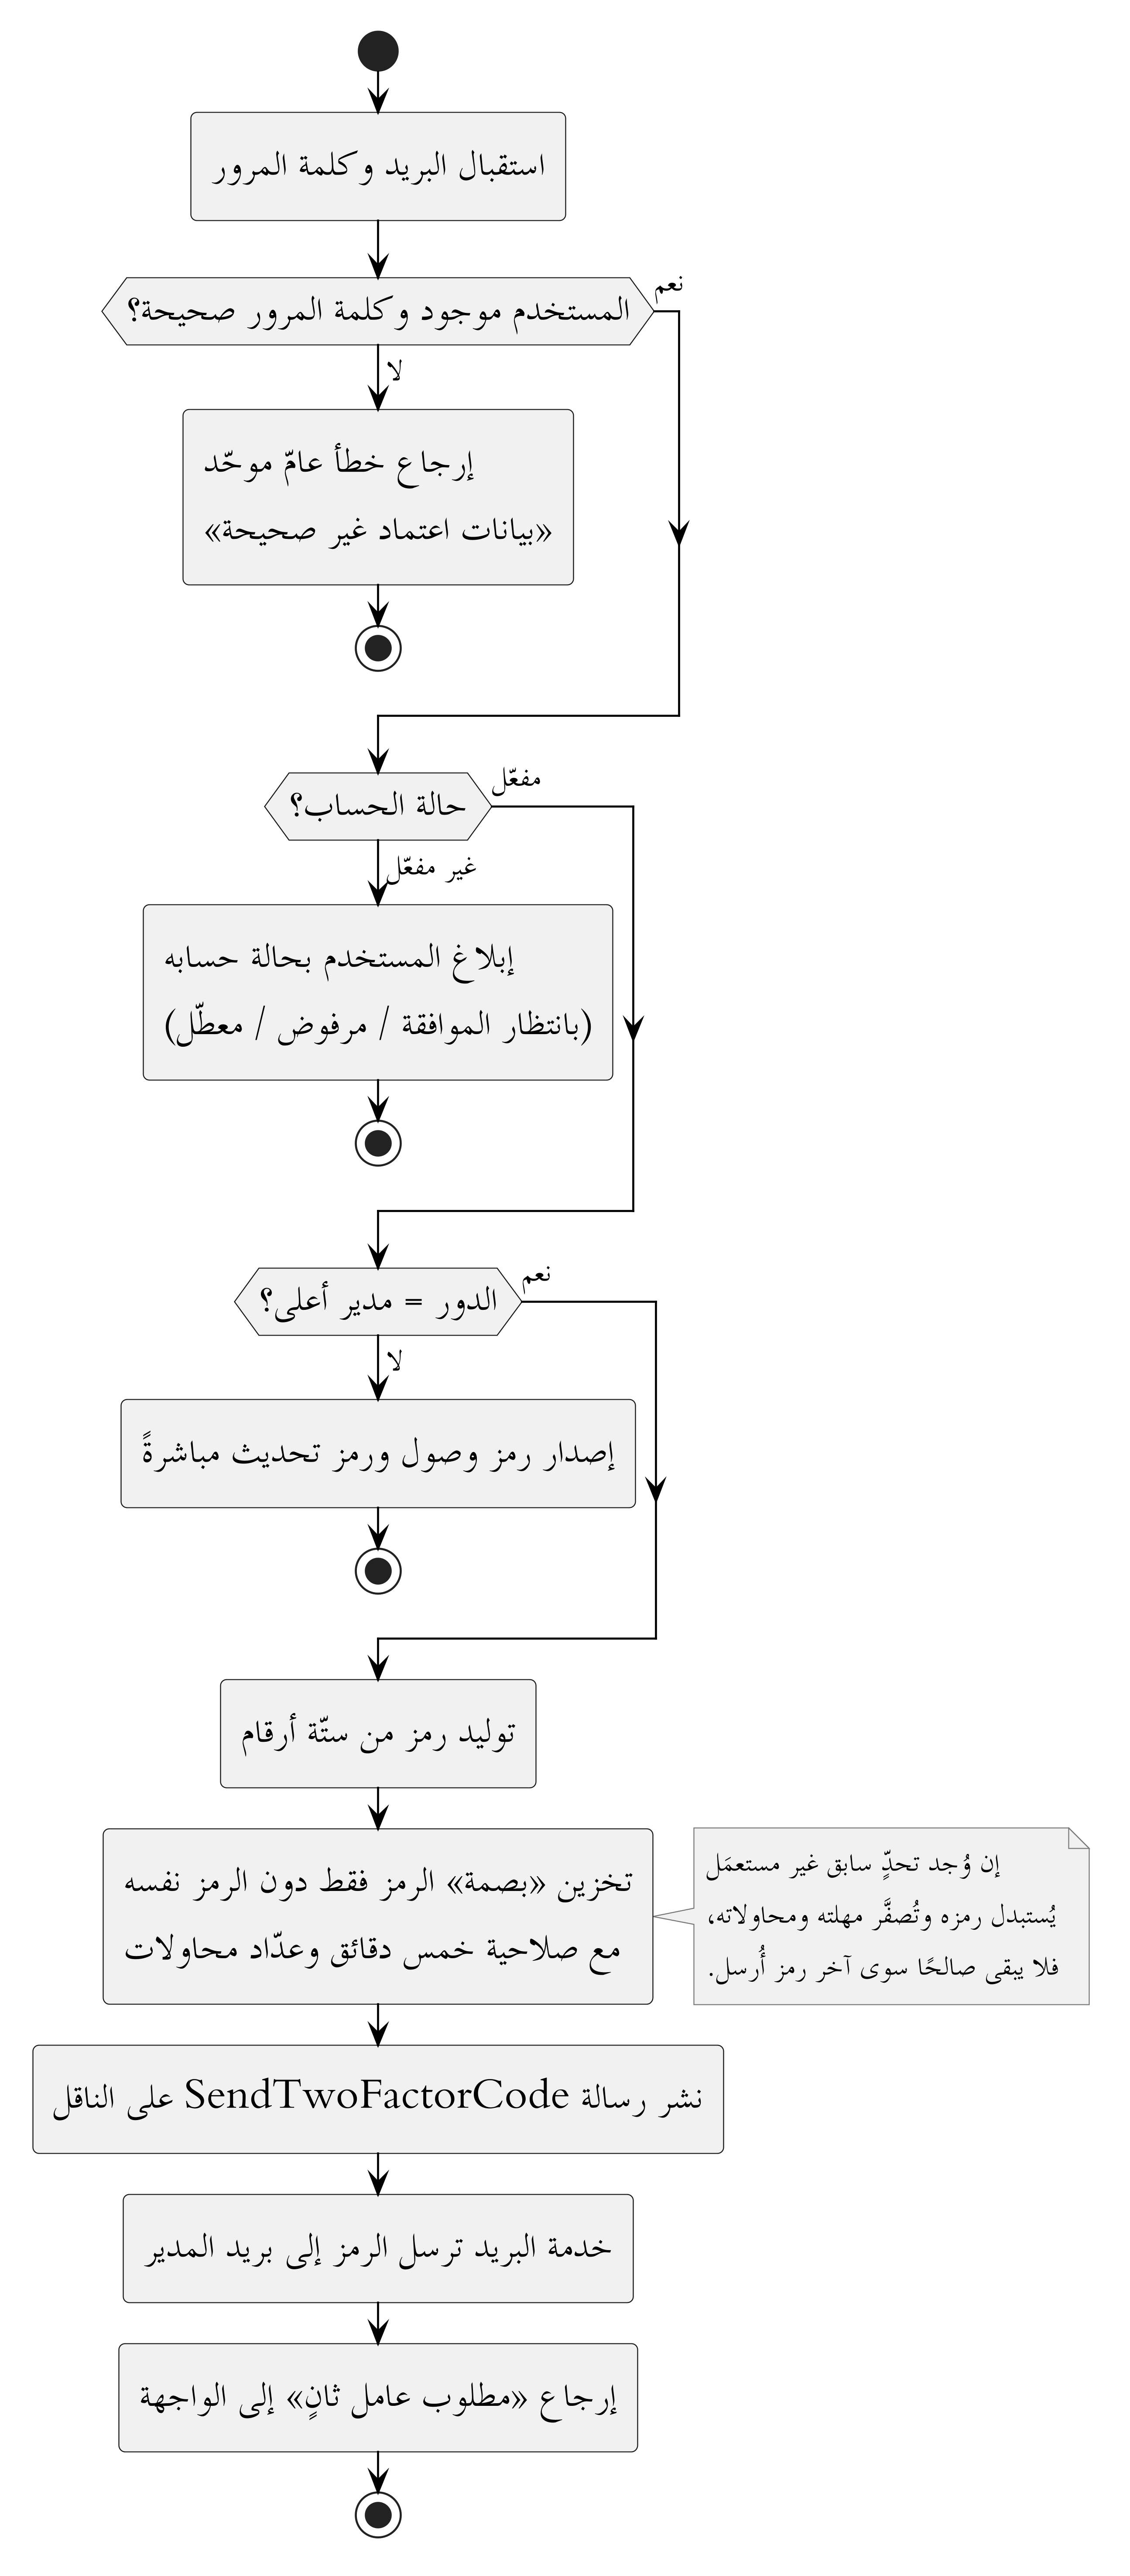
\includegraphics[width=\textwidth,height=0.8\textheight,keepaspectratio]{figures/flow-01a-two-factor-challenge.png}
  \caption{تدفّق المرحلة الأولى من تسجيل دخول المدير الأعلى: التحقّق من الاعتماد وإصدار التحدّي.}
  \label{fig:flow-01a}
\end{figure}

\begin{figure}[htbp]
  \centering
  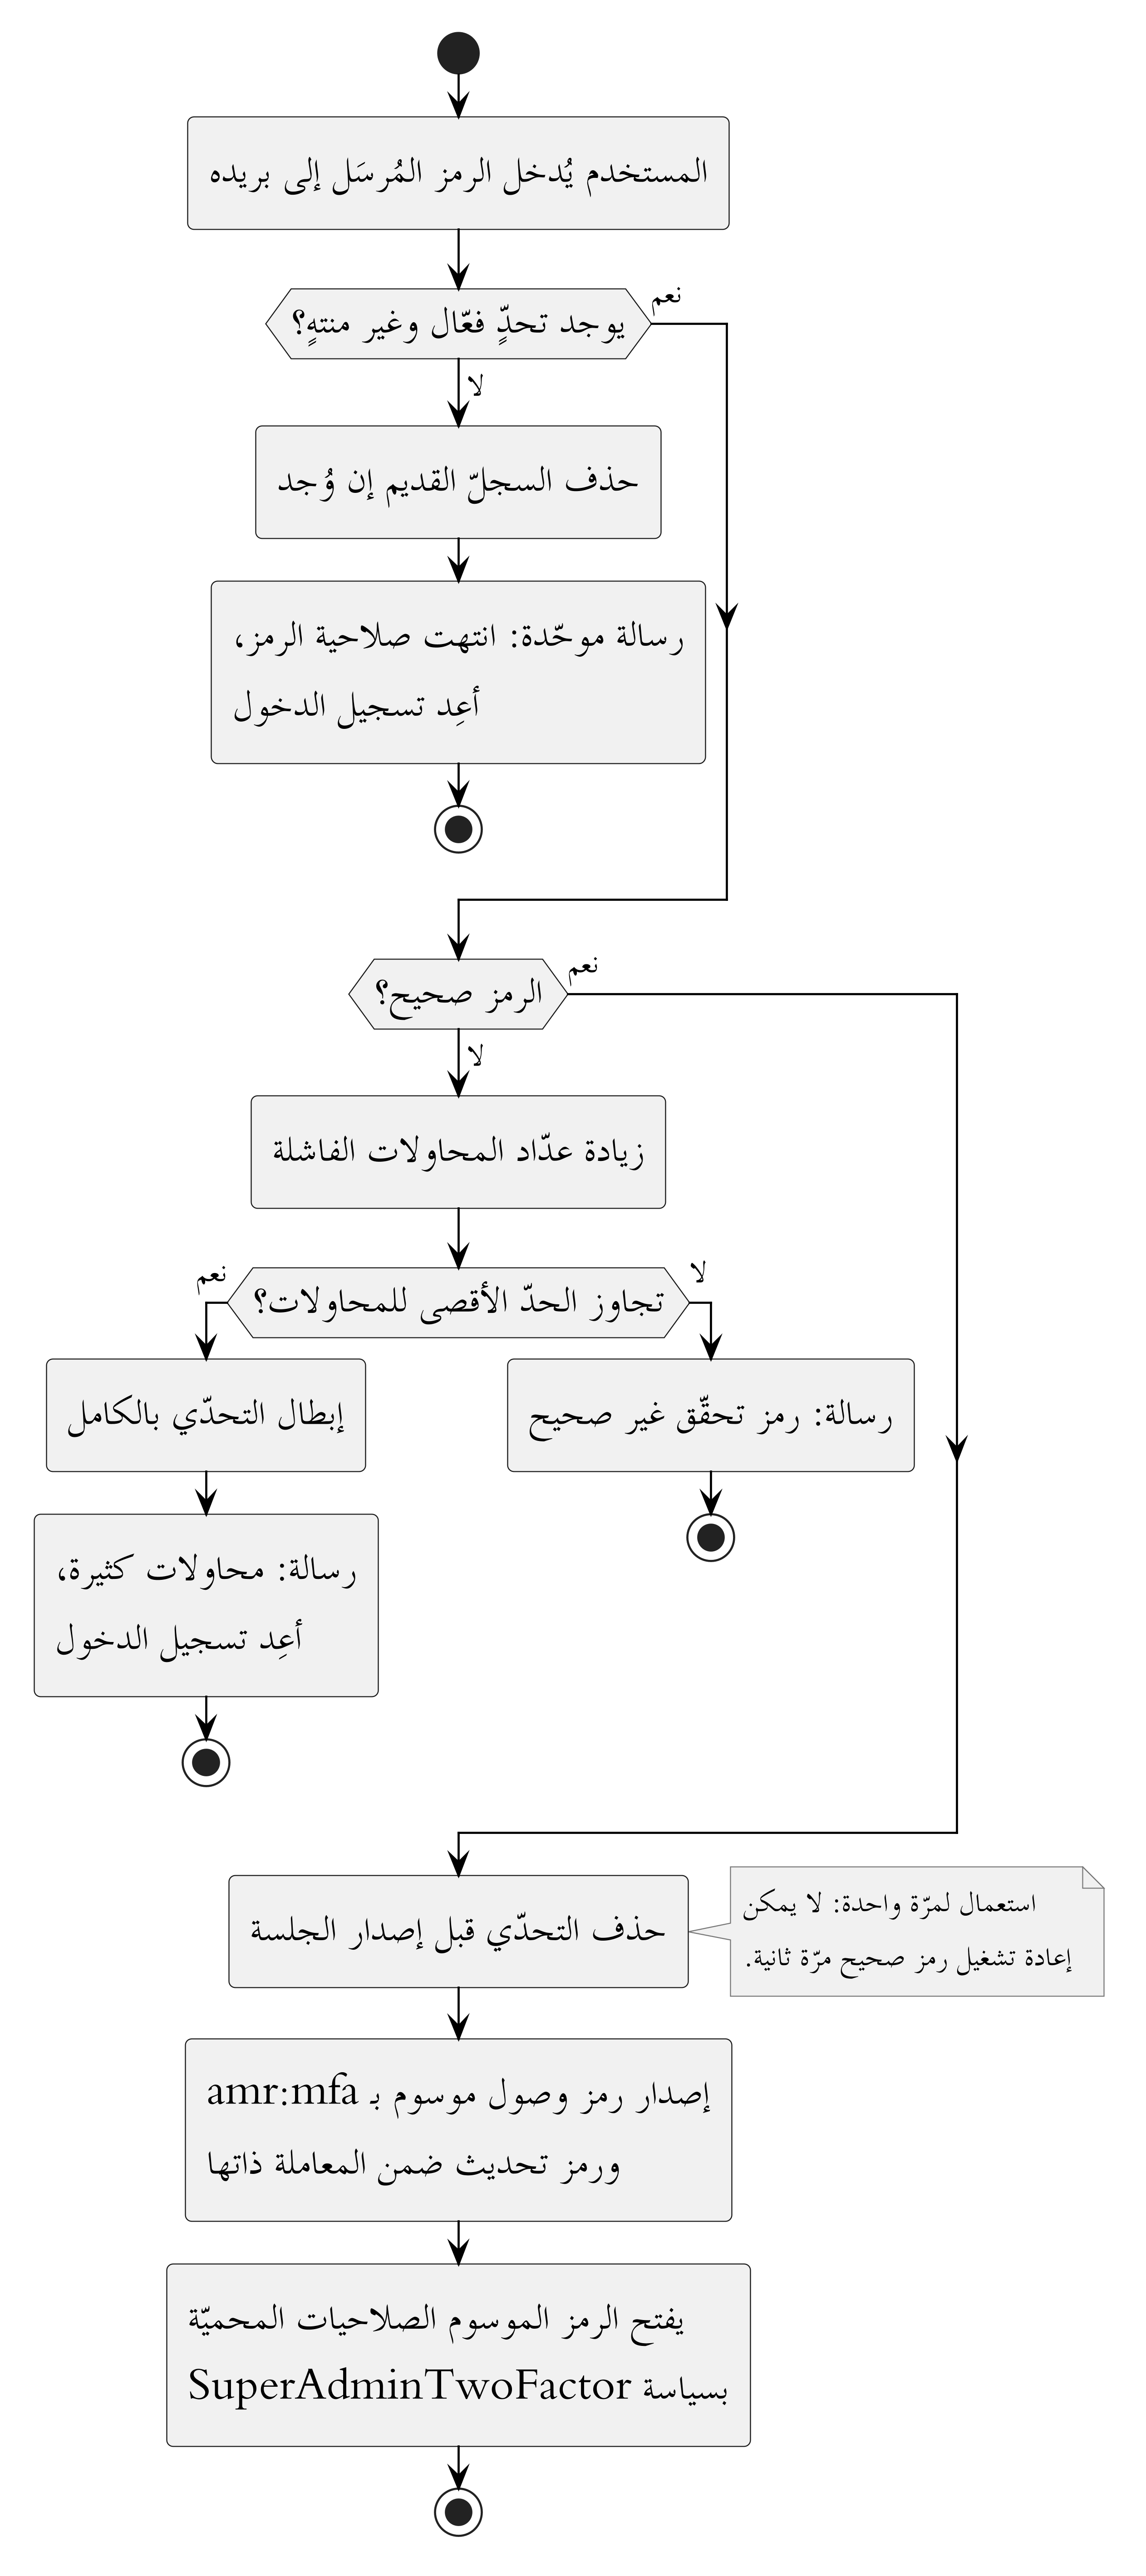
\includegraphics[width=\textwidth,height=0.8\textheight,keepaspectratio]{figures/flow-01b-two-factor-verify.png}
  \caption{تدفّق المرحلة الثانية من تسجيل دخول المدير الأعلى: التحقّق من الرمز وإصدار الجلسة.}
  \label{fig:flow-01b}
\end{figure}

\noindent يجري تسجيل دخول المدير الأعلى على مرحلتين منفصلتين بطلبين مستقلّين، بينهما تحدٍّ قصير العمر وحيد الاستعمال. وهو أكثر منطق خدمة إدارة المستخدمين تركيبًا. وقد بُيّنت مرحلتاه في الشكلين~\ref{fig:flow-01a} و\ref{fig:flow-01b}.

ويقوم هذا التدفّق على ثلاثة ضوابط أمنية:

\begin{enumerate}
  \item \textbf{توحيد رسائل الفشل}: يُرجِع النظام رسالة فشل عامّة واحدة، سواء أكان البريد غير مسجَّل أم كانت كلمة المرور خاطئة. ويمنع ذلك استعمال نقطة النهاية للكشف عن العناوين المسجَّلة في النظام.
  \item \textbf{تخزين البصمة لا الرمز}: تُحفَظ بصمة رمز العامل الثاني لا الرمز نفسه، فلا يمنح تسريب قاعدة البيانات رمزًا صالحًا للاستعمال.
  \item \textbf{حذف التحدّي قبل إصدار الجلسة}: يُحذَف سجلّ التحدّي قبل توليد الرمز، فلا يمكن إعادة استعمال رمز صحيح مرّةً ثانية.
\end{enumerate}

ويُوسَم رمز الوصول الناتج بالادّعاء \en{amr:mfa}، وهو ما تشترطه السياسة \en{SuperAdminTwoFactor} لفتح الصلاحيات الأشدّ حساسية.

\subsubsection{مخطط تسلسل النظام لحالة استعراض الجلسات والبحث فيها}

\begin{figure}[htbp]
  \centering
  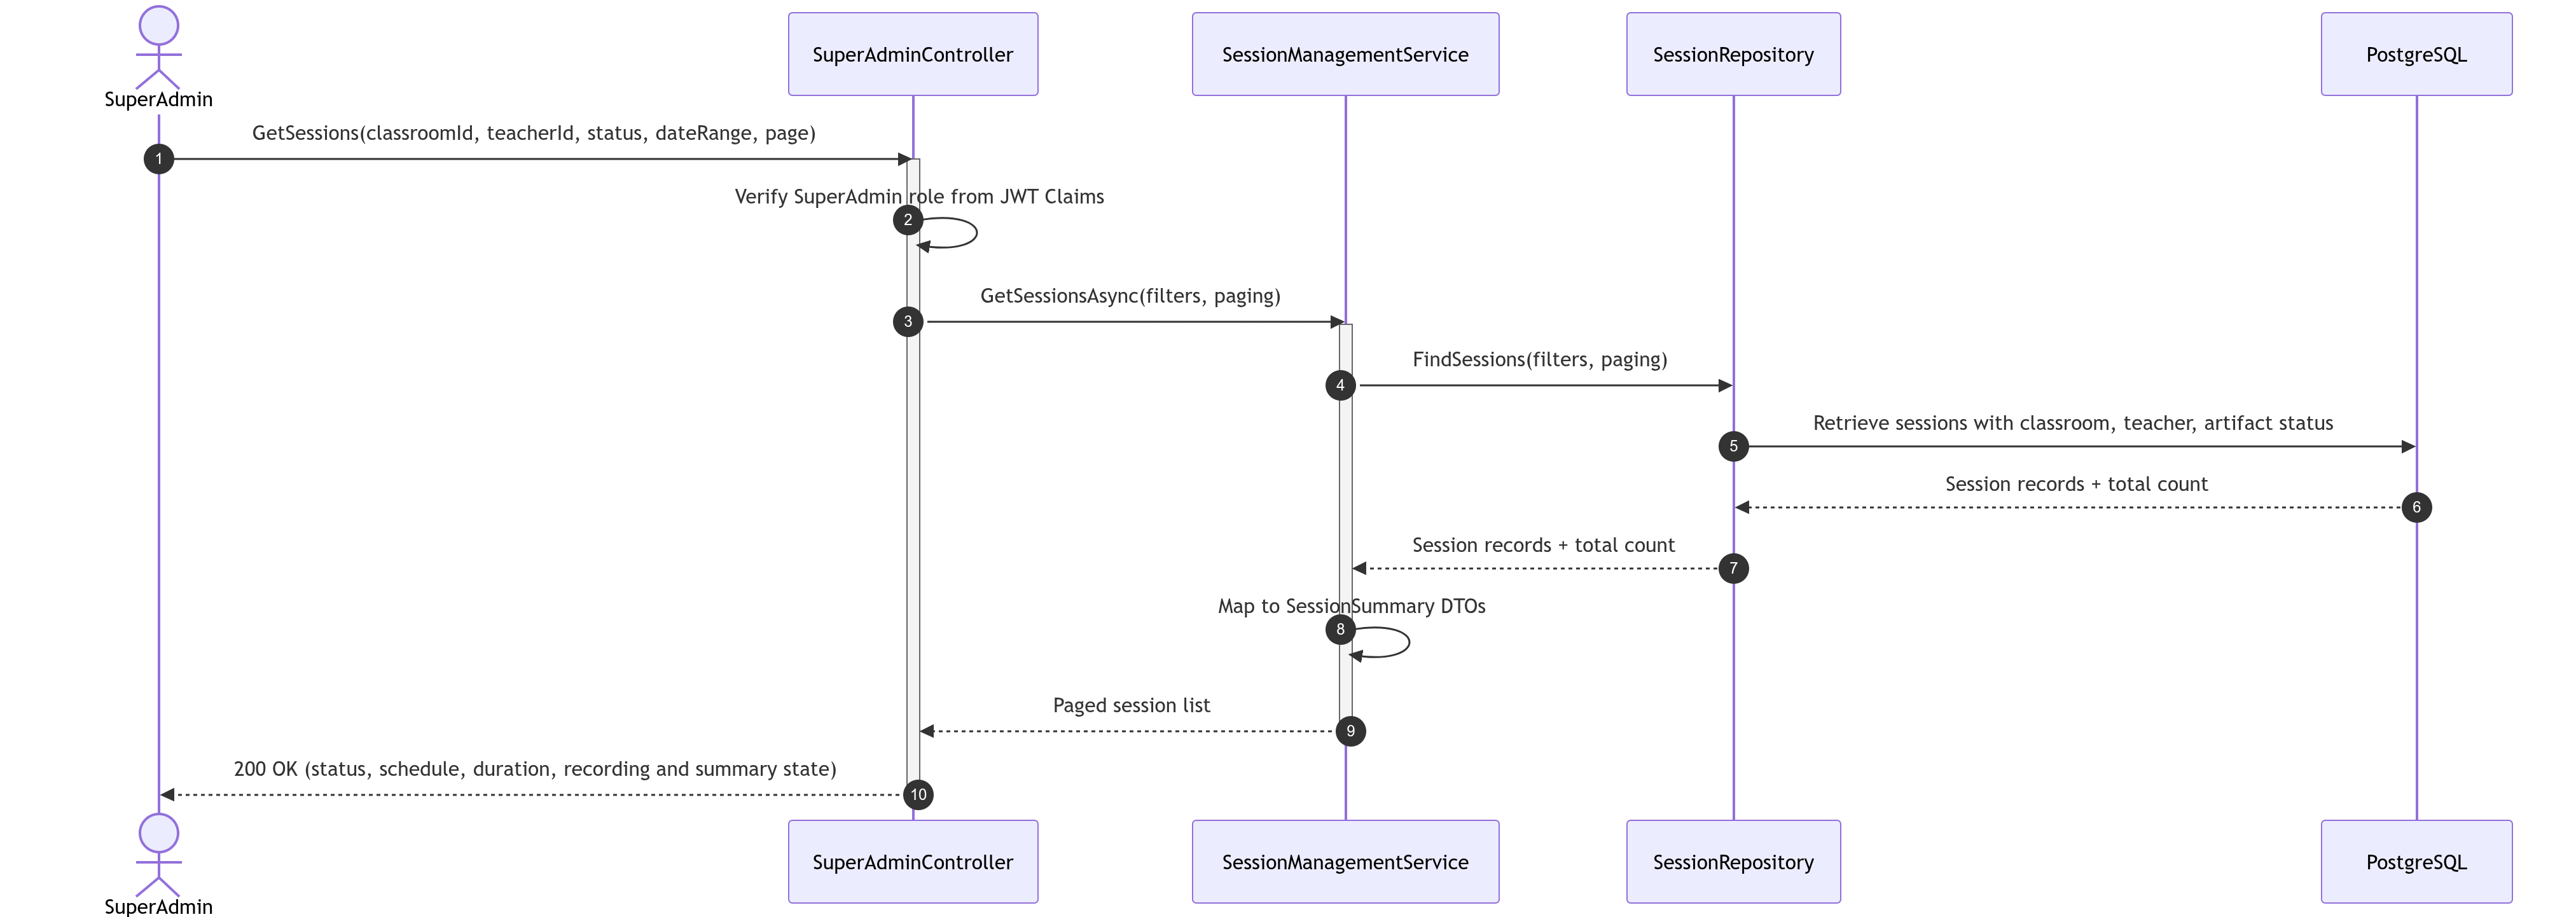
\includegraphics[width=\textwidth,height=0.8\textheight,keepaspectratio]{figures/image25.png}
  \caption{مخطط تسلسل النظام لحالة «استعراض الجلسات والبحث فيها»: يوضّح الرسائل المتبادلة بين الفاعل والنظام بوصفه صندوقًا أسود، أي دون إظهار الخدمات الداخلية التي تنفّذها.}
  \label{fig:image25}
\end{figure}

\subsubsection{مخطط تسلسل النظام لحالة عرض الجلسات الحية النشطة}

\begin{figure}[htbp]
  \centering
  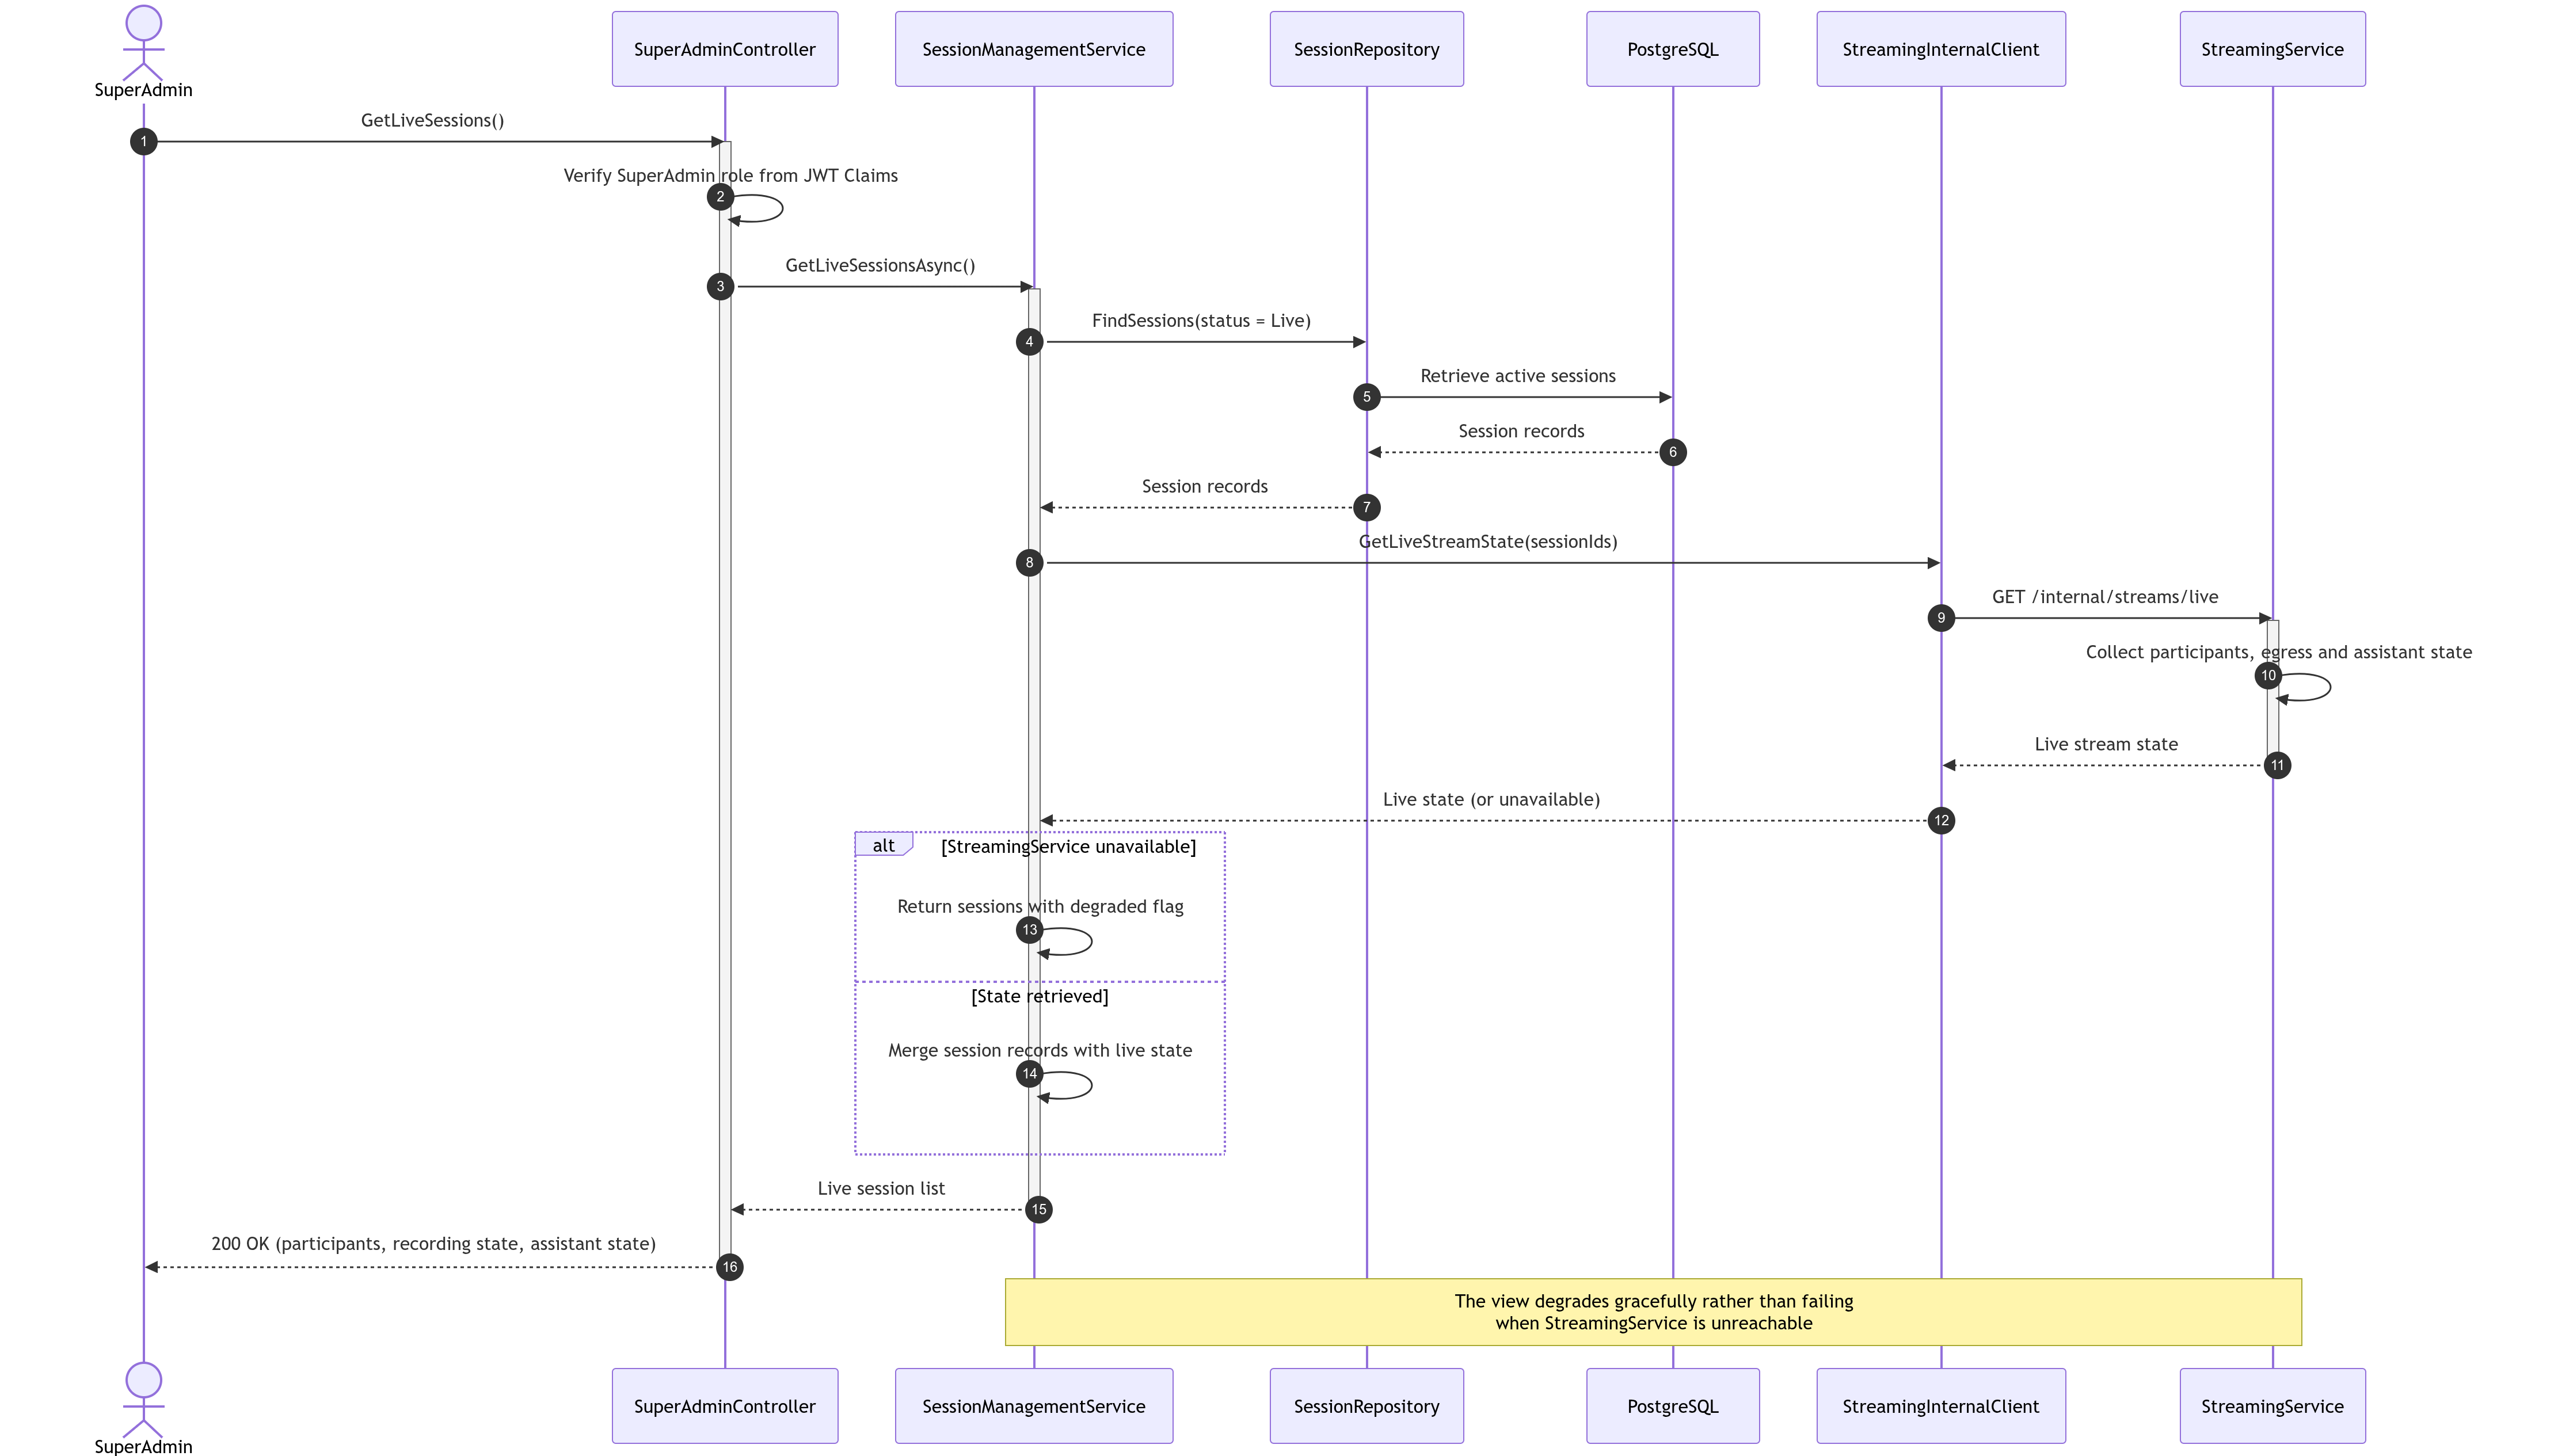
\includegraphics[width=\textwidth,height=0.8\textheight,keepaspectratio]{figures/image26.png}
  \caption{مخطط تسلسل النظام لحالة «عرض الجلسات الحية النشطة»: يوضّح الرسائل المتبادلة بين الفاعل والنظام بوصفه صندوقًا أسود، أي دون إظهار الخدمات الداخلية التي تنفّذها.}
  \label{fig:image26}
\end{figure}

\subsubsection{مخطط تسلسل النظام لحالة الإنهاء القسري لجلسة حية}

\begin{figure}[htbp]
  \centering
  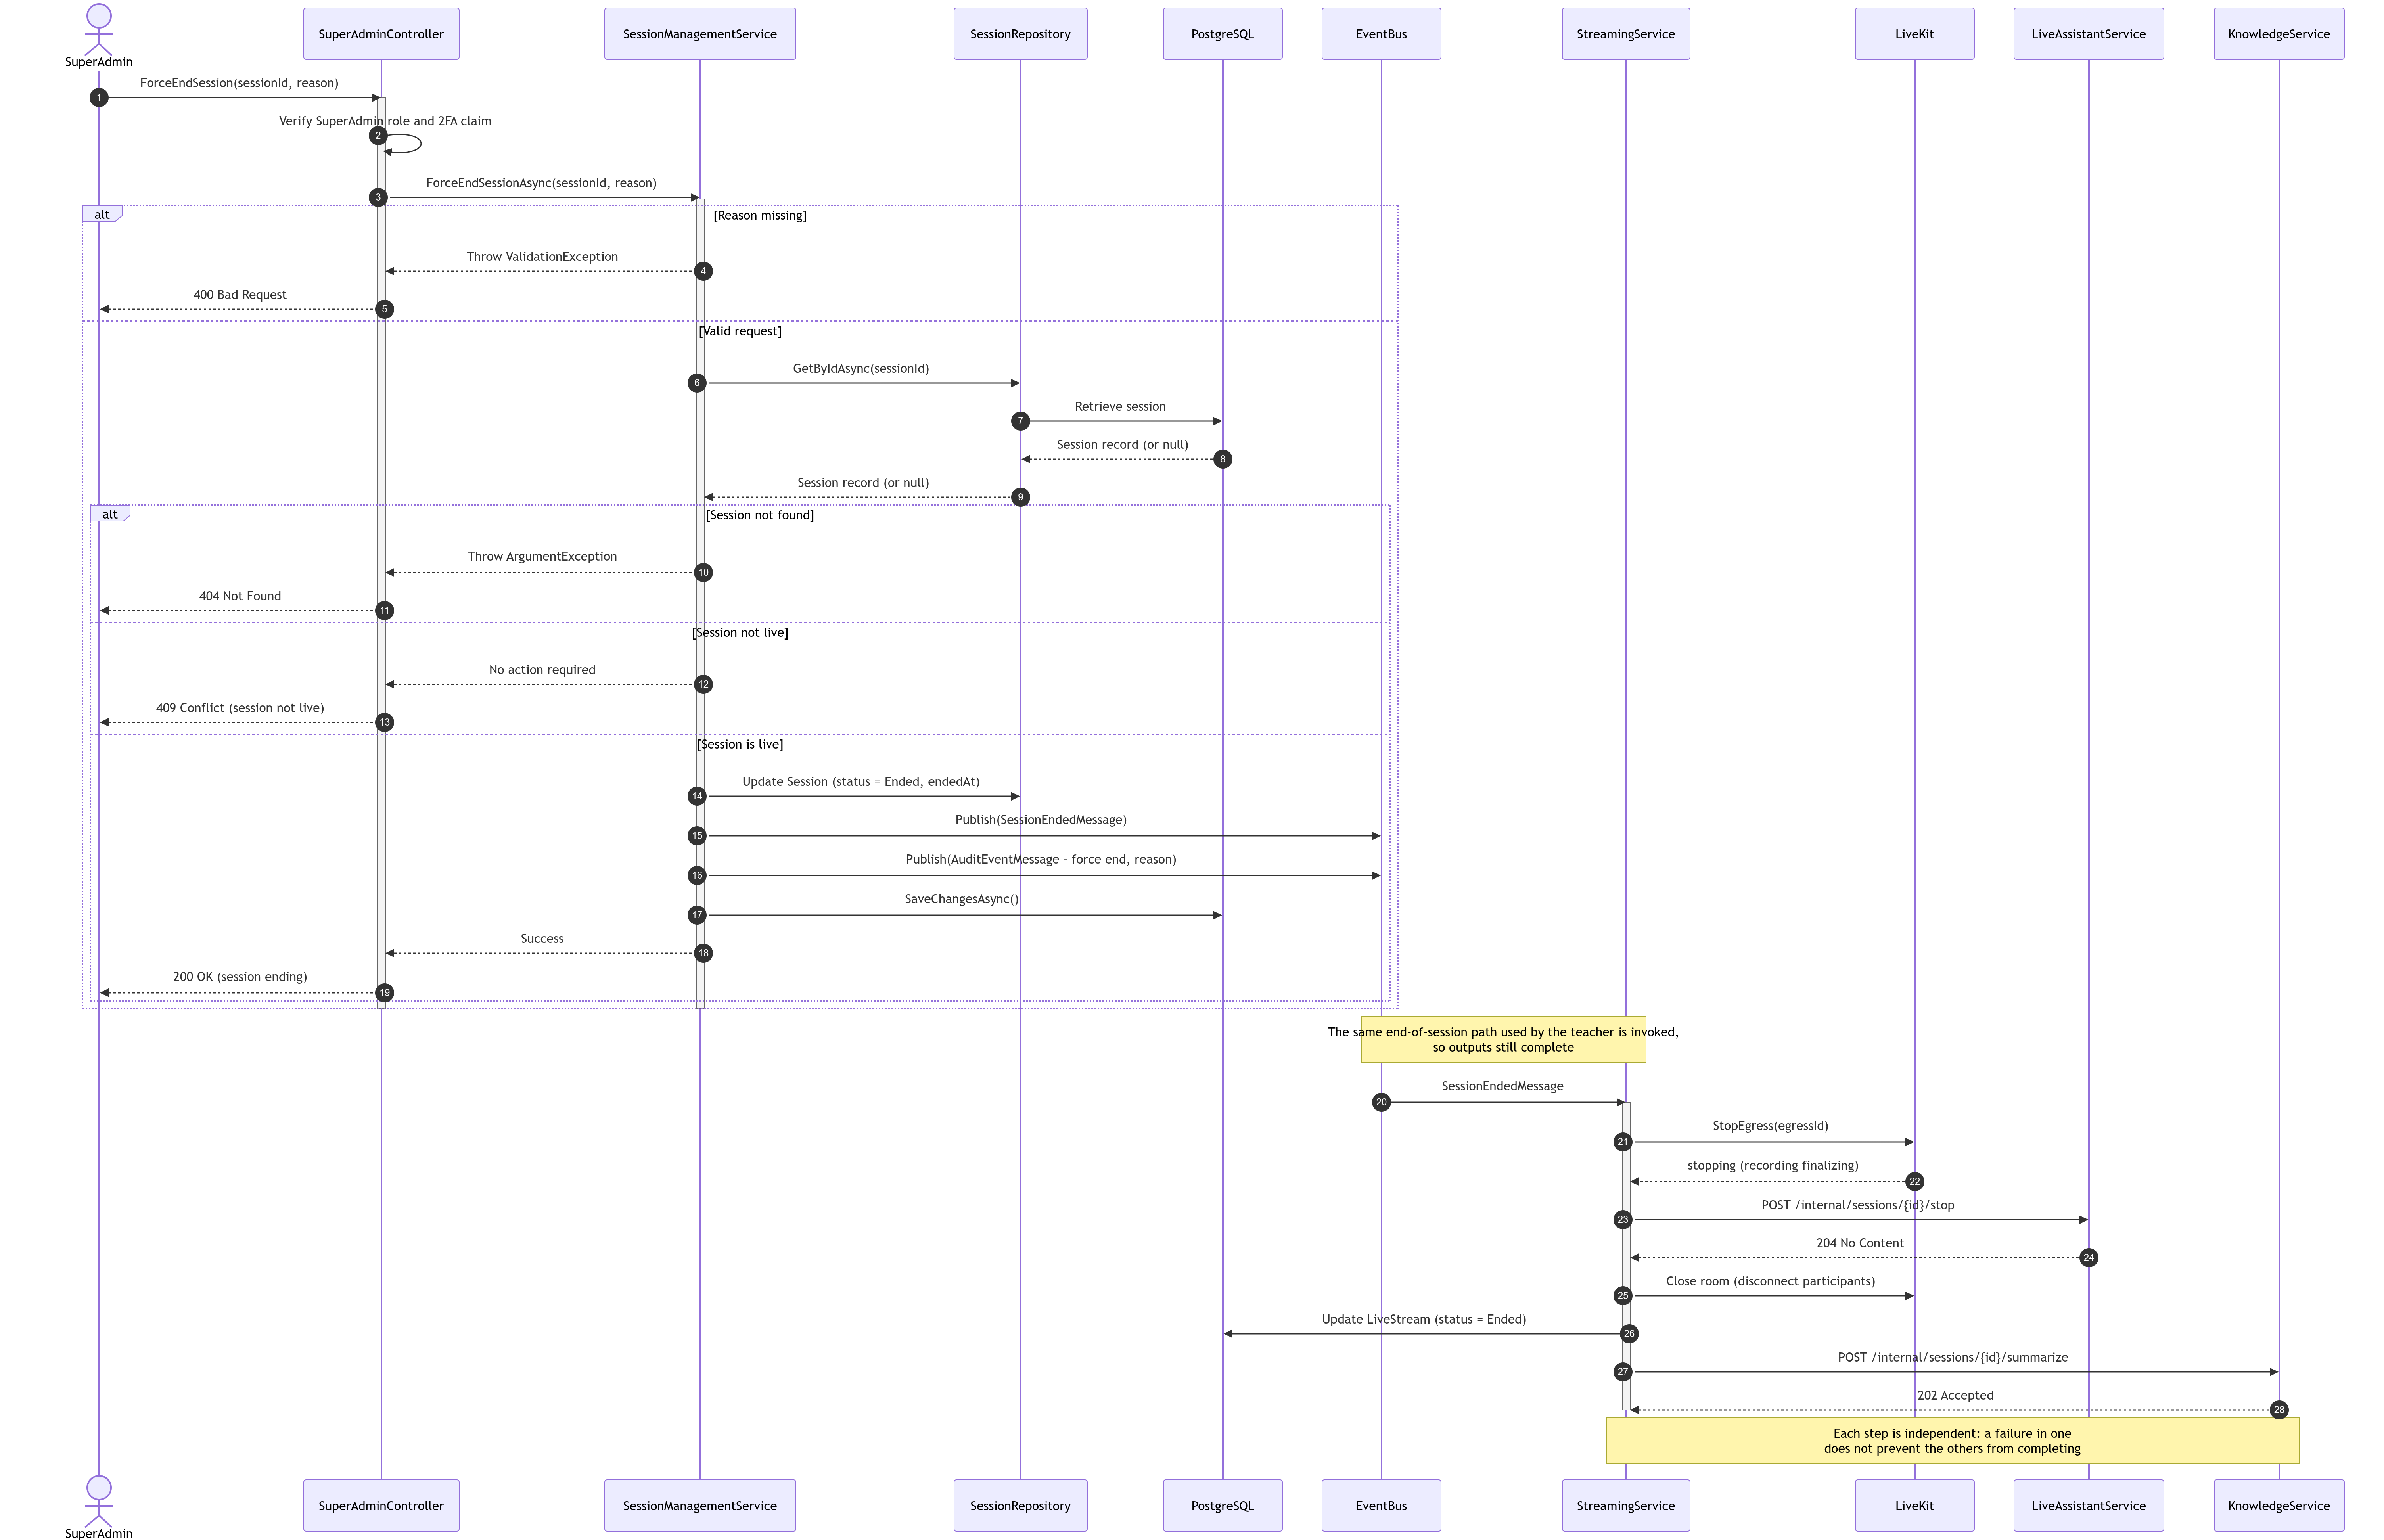
\includegraphics[width=\textwidth,height=0.8\textheight,keepaspectratio]{figures/image27.png}
  \caption{مخطط تسلسل النظام لحالة «الإنهاء القسري لجلسة حية»: يوضّح الرسائل المتبادلة بين الفاعل والنظام بوصفه صندوقًا أسود، أي دون إظهار الخدمات الداخلية التي تنفّذها.}
  \label{fig:image27}
\end{figure}

\subsection{مخطط تسلسل النظام لحالات استخدام المعلم}

\subsubsection{مخطط تسلسل النظام لحالة بدء المعلم لجلسة تعلم مباشرة}

\begin{figure}[htbp]
  \centering
  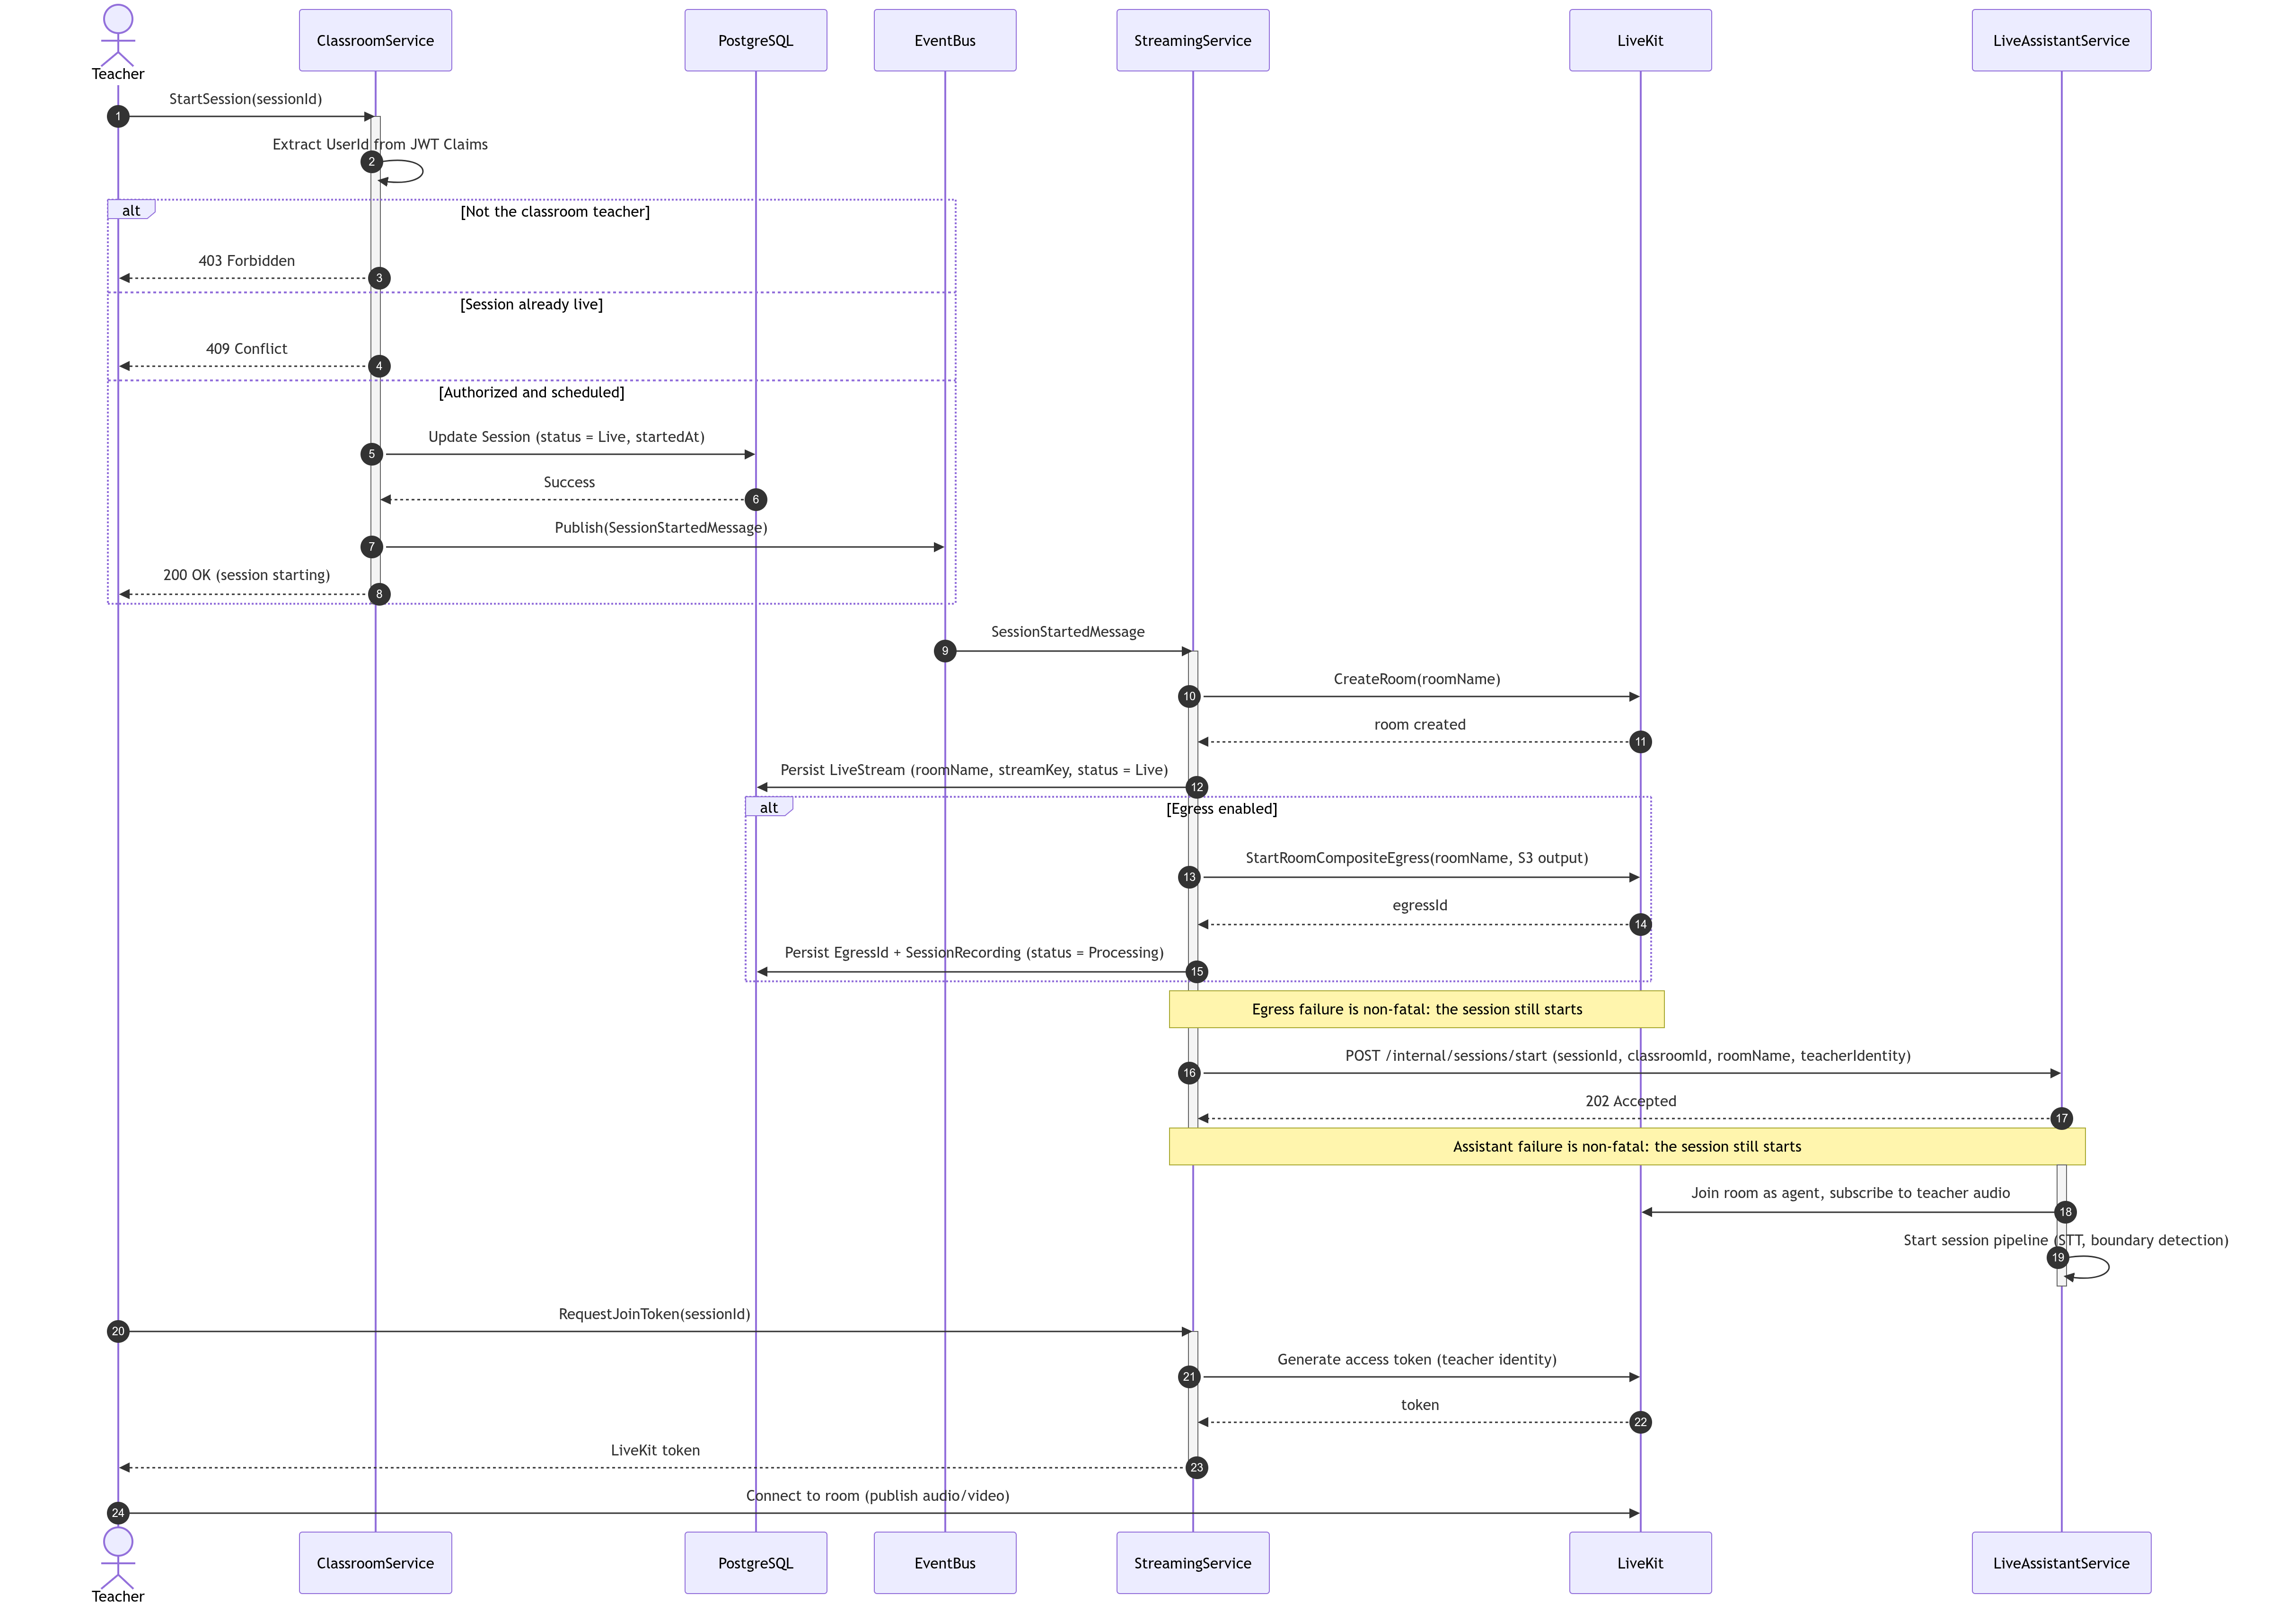
\includegraphics[width=\textwidth,height=0.8\textheight,keepaspectratio]{figures/image30.png}
  \caption{مخطط تسلسل النظام لحالة «بدء المعلم لجلسة تعلم مباشرة»: يوضّح الرسائل المتبادلة بين الفاعل والنظام بوصفه صندوقًا أسود، أي دون إظهار الخدمات الداخلية التي تنفّذها.}
  \label{fig:image30}
\end{figure}

\subsubsection{مخطط تسلسل النظام لحالة إنهاء المعلم لجلسة تعلم مباشرة}

\begin{figure}[htbp]
  \centering
  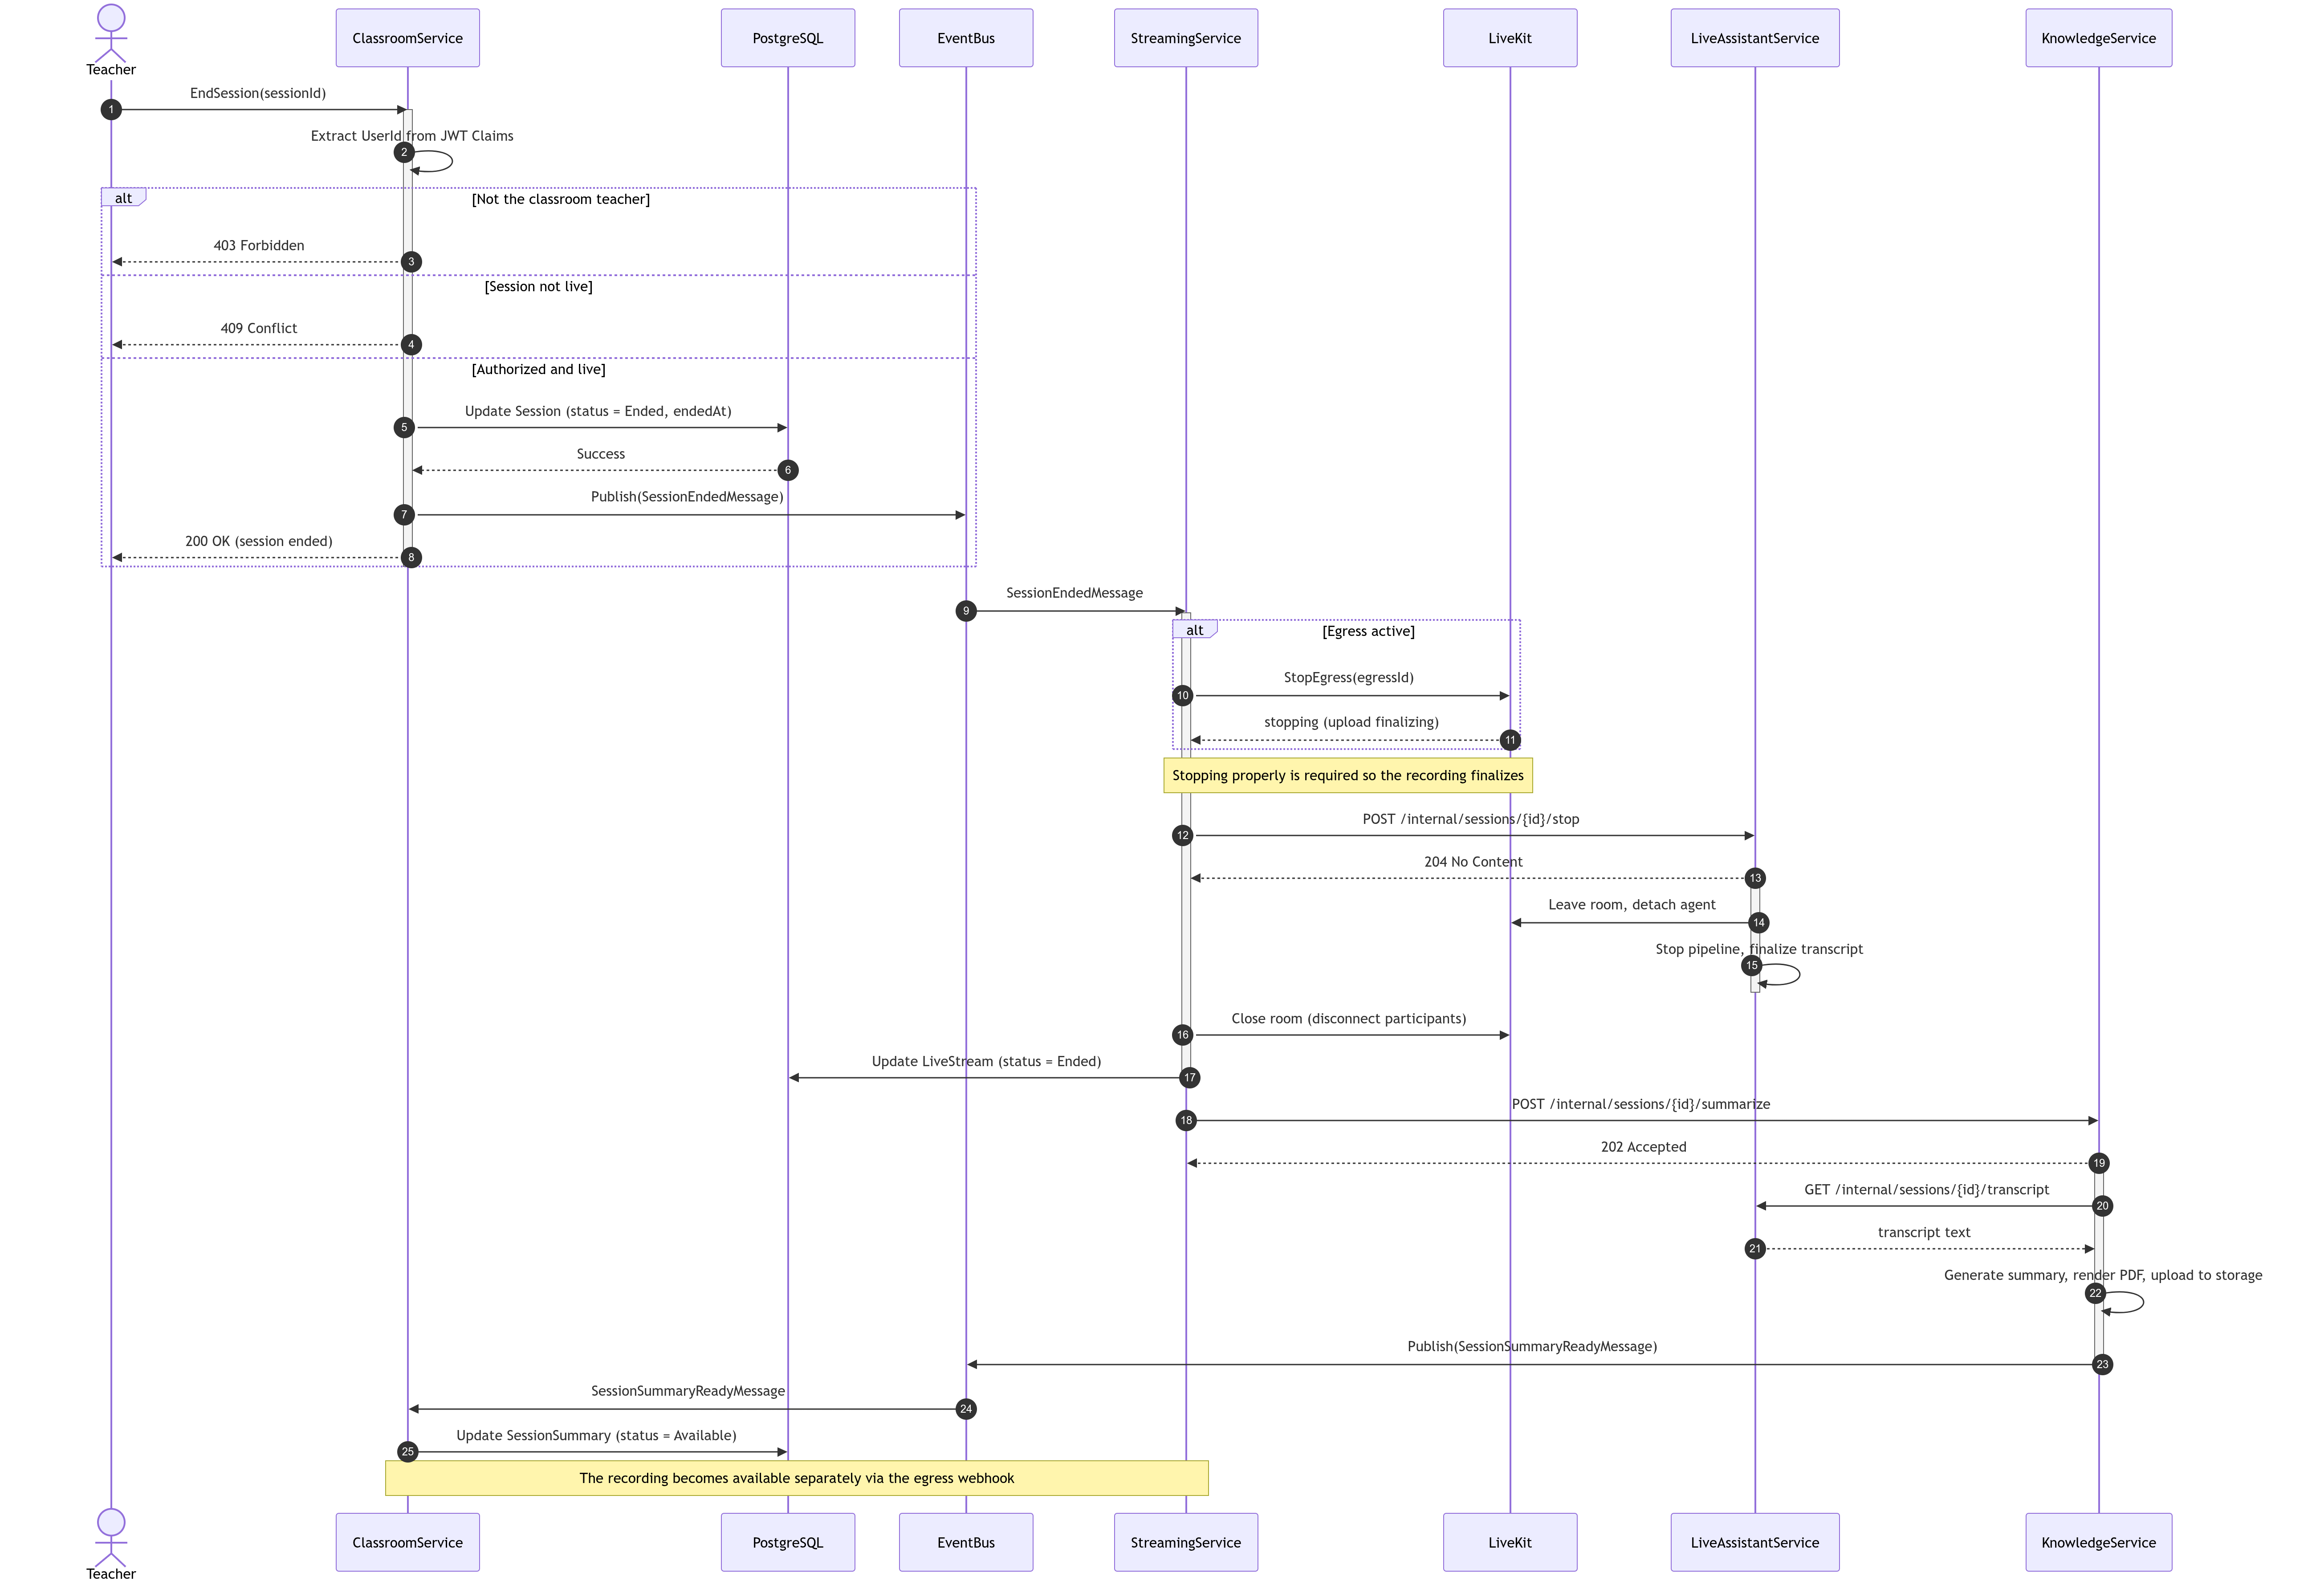
\includegraphics[width=\textwidth,height=0.8\textheight,keepaspectratio]{figures/image31.png}
  \caption{مخطط تسلسل النظام لحالة «إنهاء المعلم لجلسة تعلم مباشرة»: يوضّح الرسائل المتبادلة بين الفاعل والنظام بوصفه صندوقًا أسود، أي دون إظهار الخدمات الداخلية التي تنفّذها.}
  \label{fig:image31}
\end{figure}

\subsubsection{تدفّق إنهاء الجلسة}
\label{subsubsec:flow-session-end}

يبيّن الشكل~\ref{fig:flow-02} تدفّق إنهاء الجلسة الحيّة وما يعالجه من مشكلات السباق والذرّية والترتيب.

\begin{figure}[htbp]
  \centering
  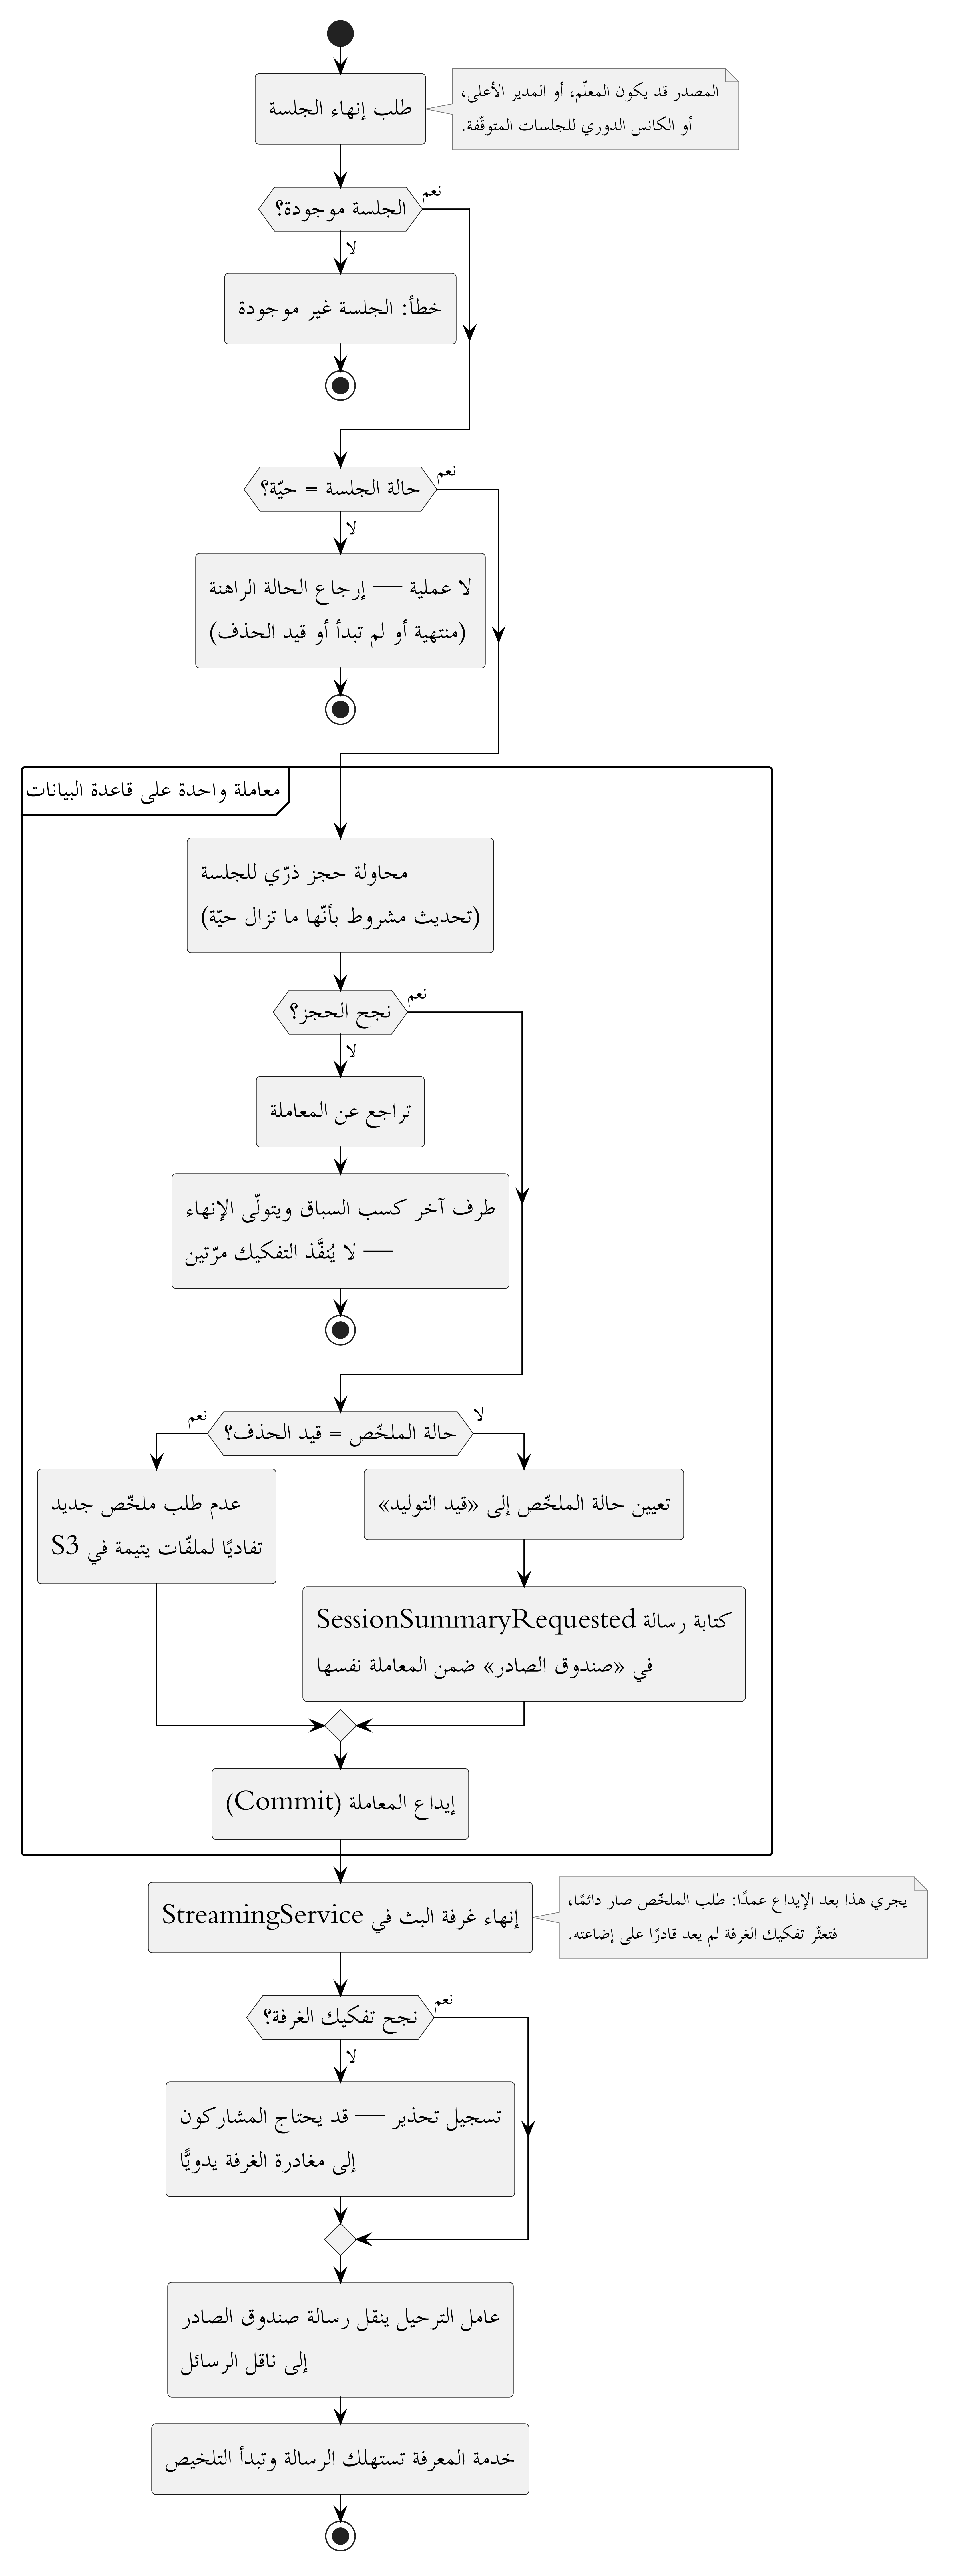
\includegraphics[width=\textwidth,height=0.8\textheight,keepaspectratio]{figures/flow-02-session-lifecycle.png}
  \caption{تدفّق إنهاء الجلسة الحيّة في خدمة الفصول الدراسية.}
  \label{fig:flow-02}
\end{figure}

\noindent تجتمع في إجرائية إنهاء الجلسة الحيّة ثلاث مشكلات صحّة منفصلة، وهي أعقد منطق في خدمة الفصول الدراسية. وقد بُيّن هذا التدفّق في الشكل~\ref{fig:flow-02}.

\begin{enumerate}
  \item \textbf{السباق} (\en{Race Condition}): يمكن أن تُنهى الجلسة من المعلّم أو المدير الأعلى أو الكانس الدوري في اللحظة نفسها. واستُعمل تحديثٌ ذرّيٌّ مشروط يُسنِد الفصل في التزامن إلى قاعدة البيانات: يتولّى التفكيك من ينجح في الحجز، ويتوقّف من يفشل فيه، فلا يُنفَّذ التفكيك مرّتين.
  \item \textbf{الذرّية} (\en{Atomicity}): يجب أن يُحفَظ تغيّرُ حالة الجلسة وتسجيلُ استحقاق الملخّص معًا أو لا يُحفَظ أيٌّ منهما. ولذلك تُكتَب رسالة طلب الملخّص في جدول صندوق الصادر ضمن المعاملة نفسها، ثمّ يُرحّلها عاملٌ مستقلّ إلى الناقل لاحقًا، بدلًا من نشرها مباشرةً.
  \item \textbf{الترتيب} (\en{Ordering}): يجري تفكيك غرفة البث بعد إيداع المعاملة. ويُبنى الملخّص من النصّ الذي يُفرِغه المساعد المباشر عند التفكيك، وقد صار طلب الملخّص محفوظًا في قاعدة البيانات قبل ذلك. ولا يؤدّي بطء تفكيك الغرفة أو تعثّره عندئذٍ إلى فقد الملخّص.
\end{enumerate}

\subsubsection{مخطط تسلسل النظام لحالة انضمام الطالب إلى جلسة تعلم مباشرة}

\begin{figure}[htbp]
  \centering
  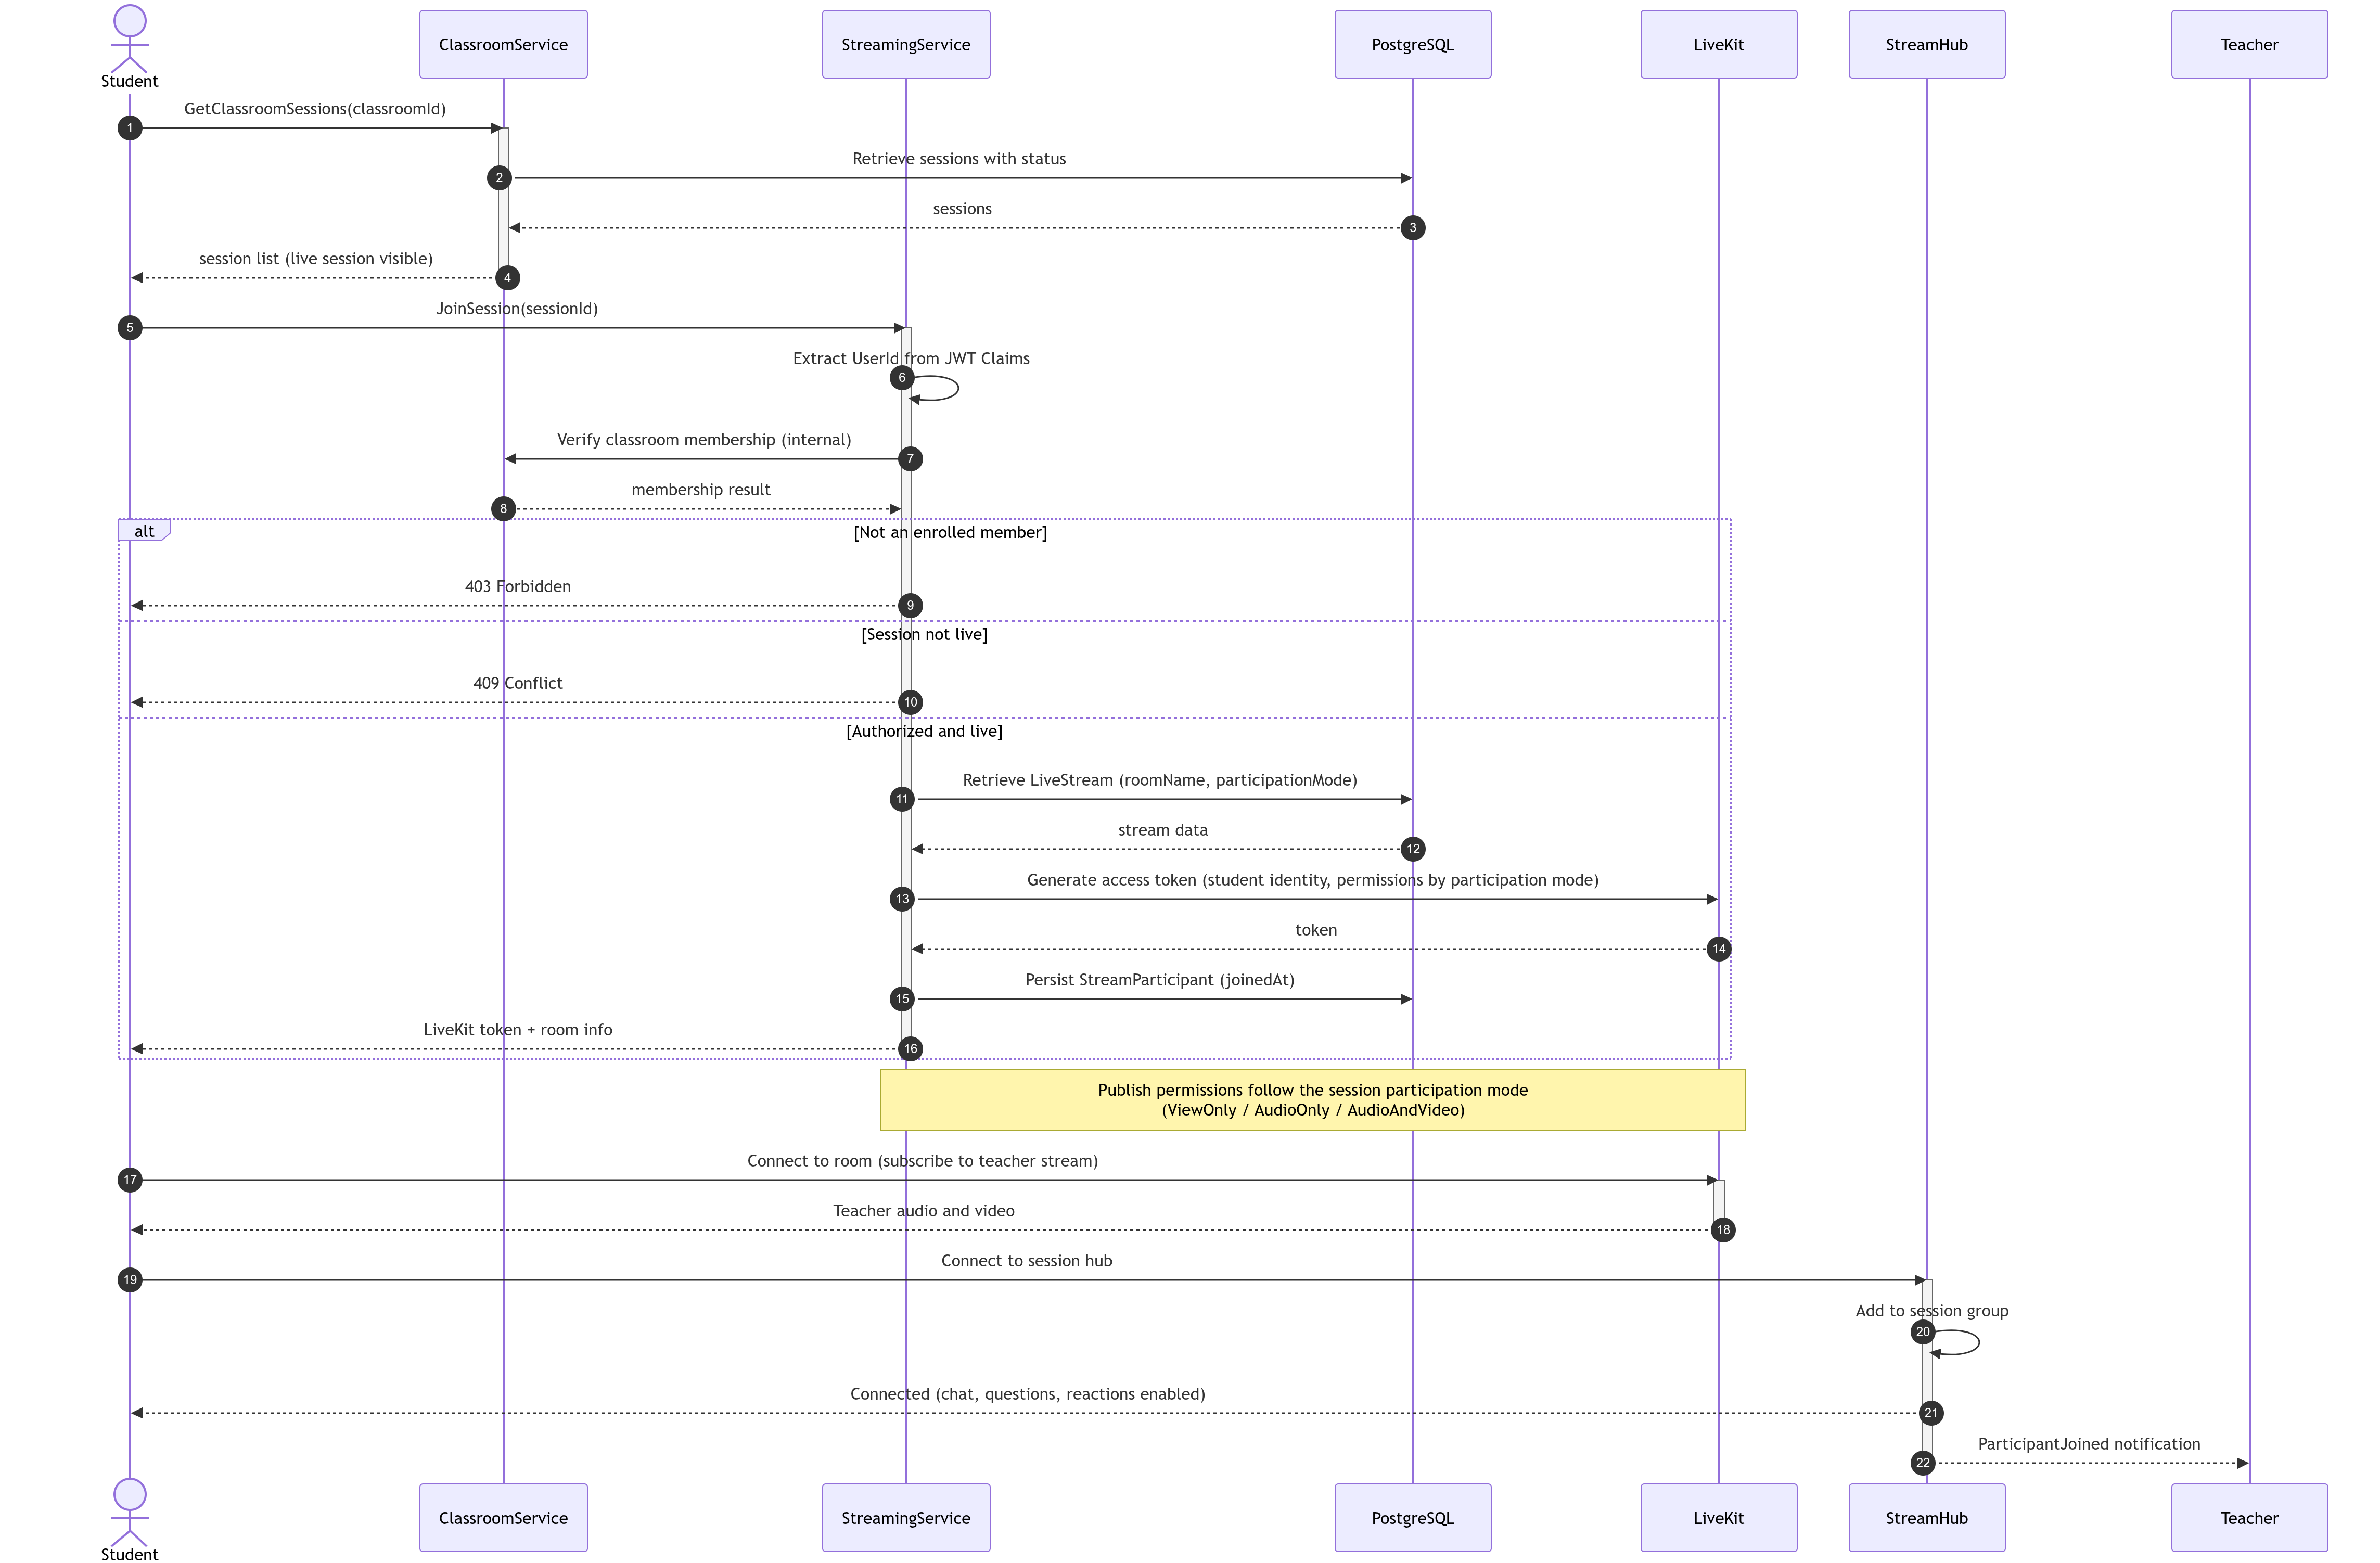
\includegraphics[width=\textwidth,height=0.8\textheight,keepaspectratio]{figures/image32.png}
  \caption{مخطط تسلسل النظام لحالة «انضمام الطالب إلى جلسة تعلم مباشرة»: يوضّح الرسائل المتبادلة بين الفاعل والنظام بوصفه صندوقًا أسود، أي دون إظهار الخدمات الداخلية التي تنفّذها.}
  \label{fig:image32}
\end{figure}

\subsubsection{مخطط تسلسل النظام لحالة التفاعل داخل جلسة التعلم المباشرة}

\begin{figure}[htbp]
  \centering
  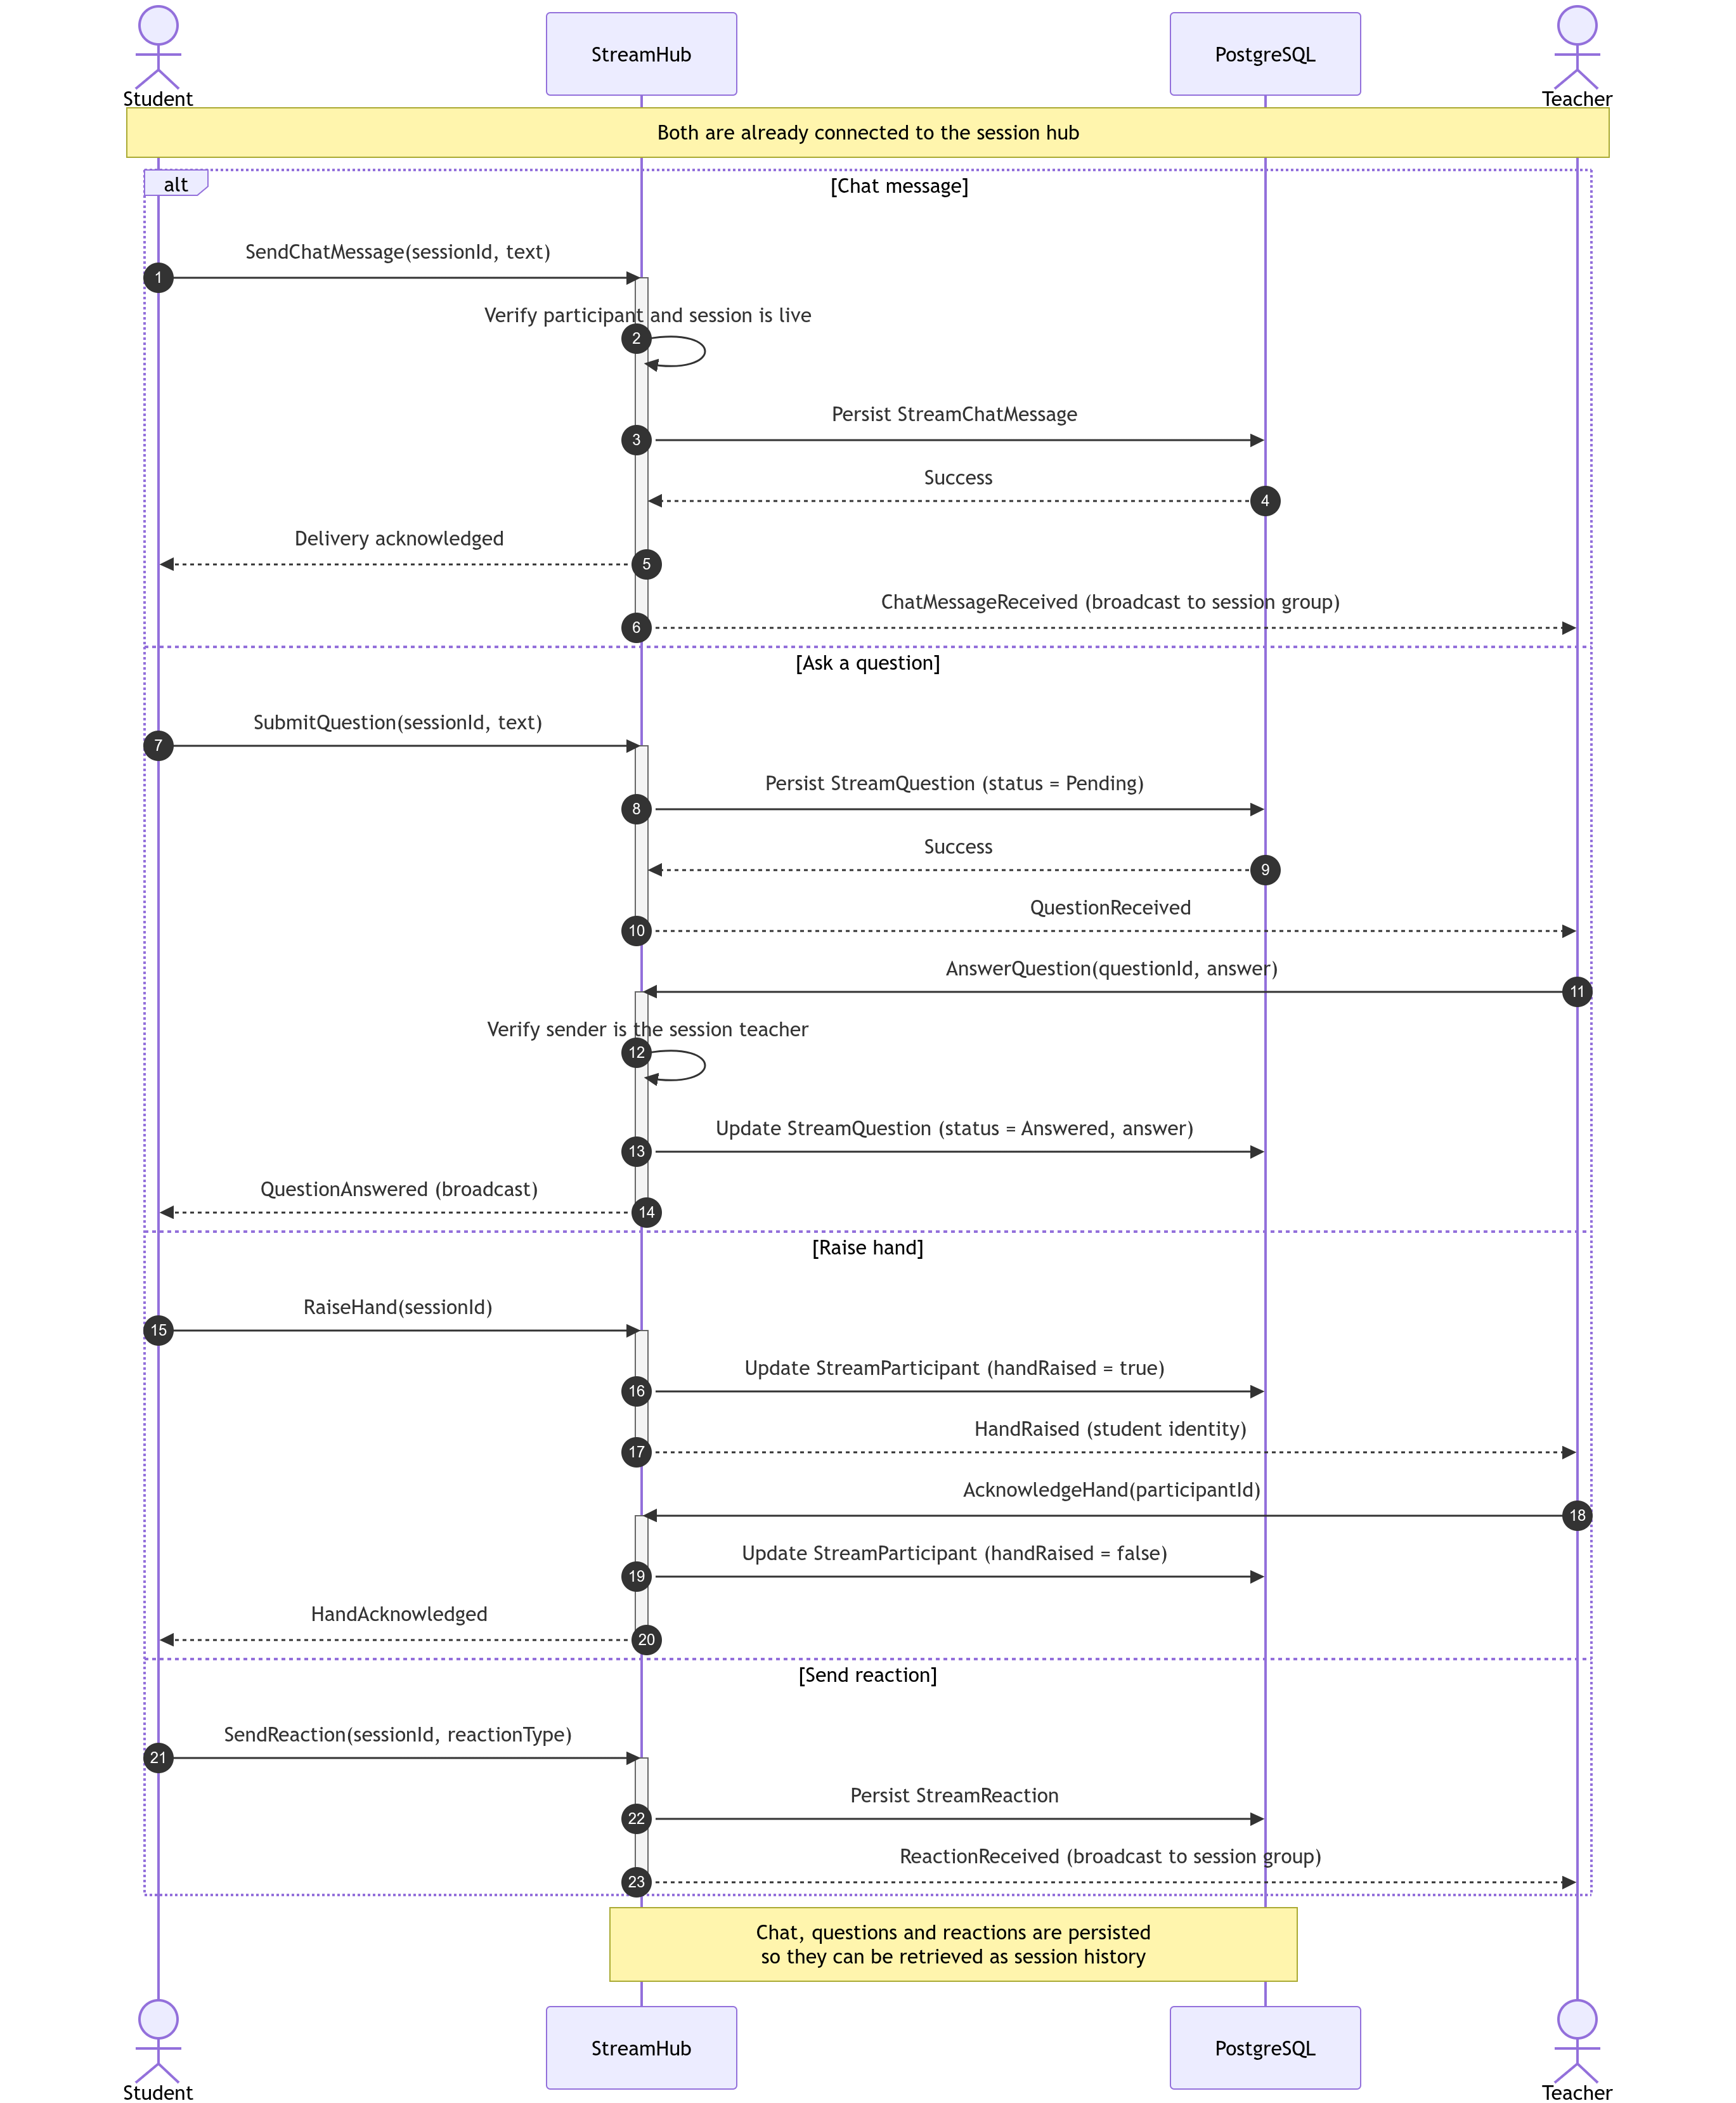
\includegraphics[width=\textwidth,height=0.8\textheight,keepaspectratio]{figures/image33.png}
  \caption{مخطط تسلسل النظام لحالة «التفاعل داخل جلسة التعلم المباشرة»: يوضّح الرسائل المتبادلة بين الفاعل والنظام بوصفه صندوقًا أسود، أي دون إظهار الخدمات الداخلية التي تنفّذها.}
  \label{fig:image33}
\end{figure}

\subsubsection{مخطط تسلسل النظام لحالة الإجابة عن سؤال الطالب اعتمادًا على مواد الفصل}

\begin{figure}[htbp]
  \centering
  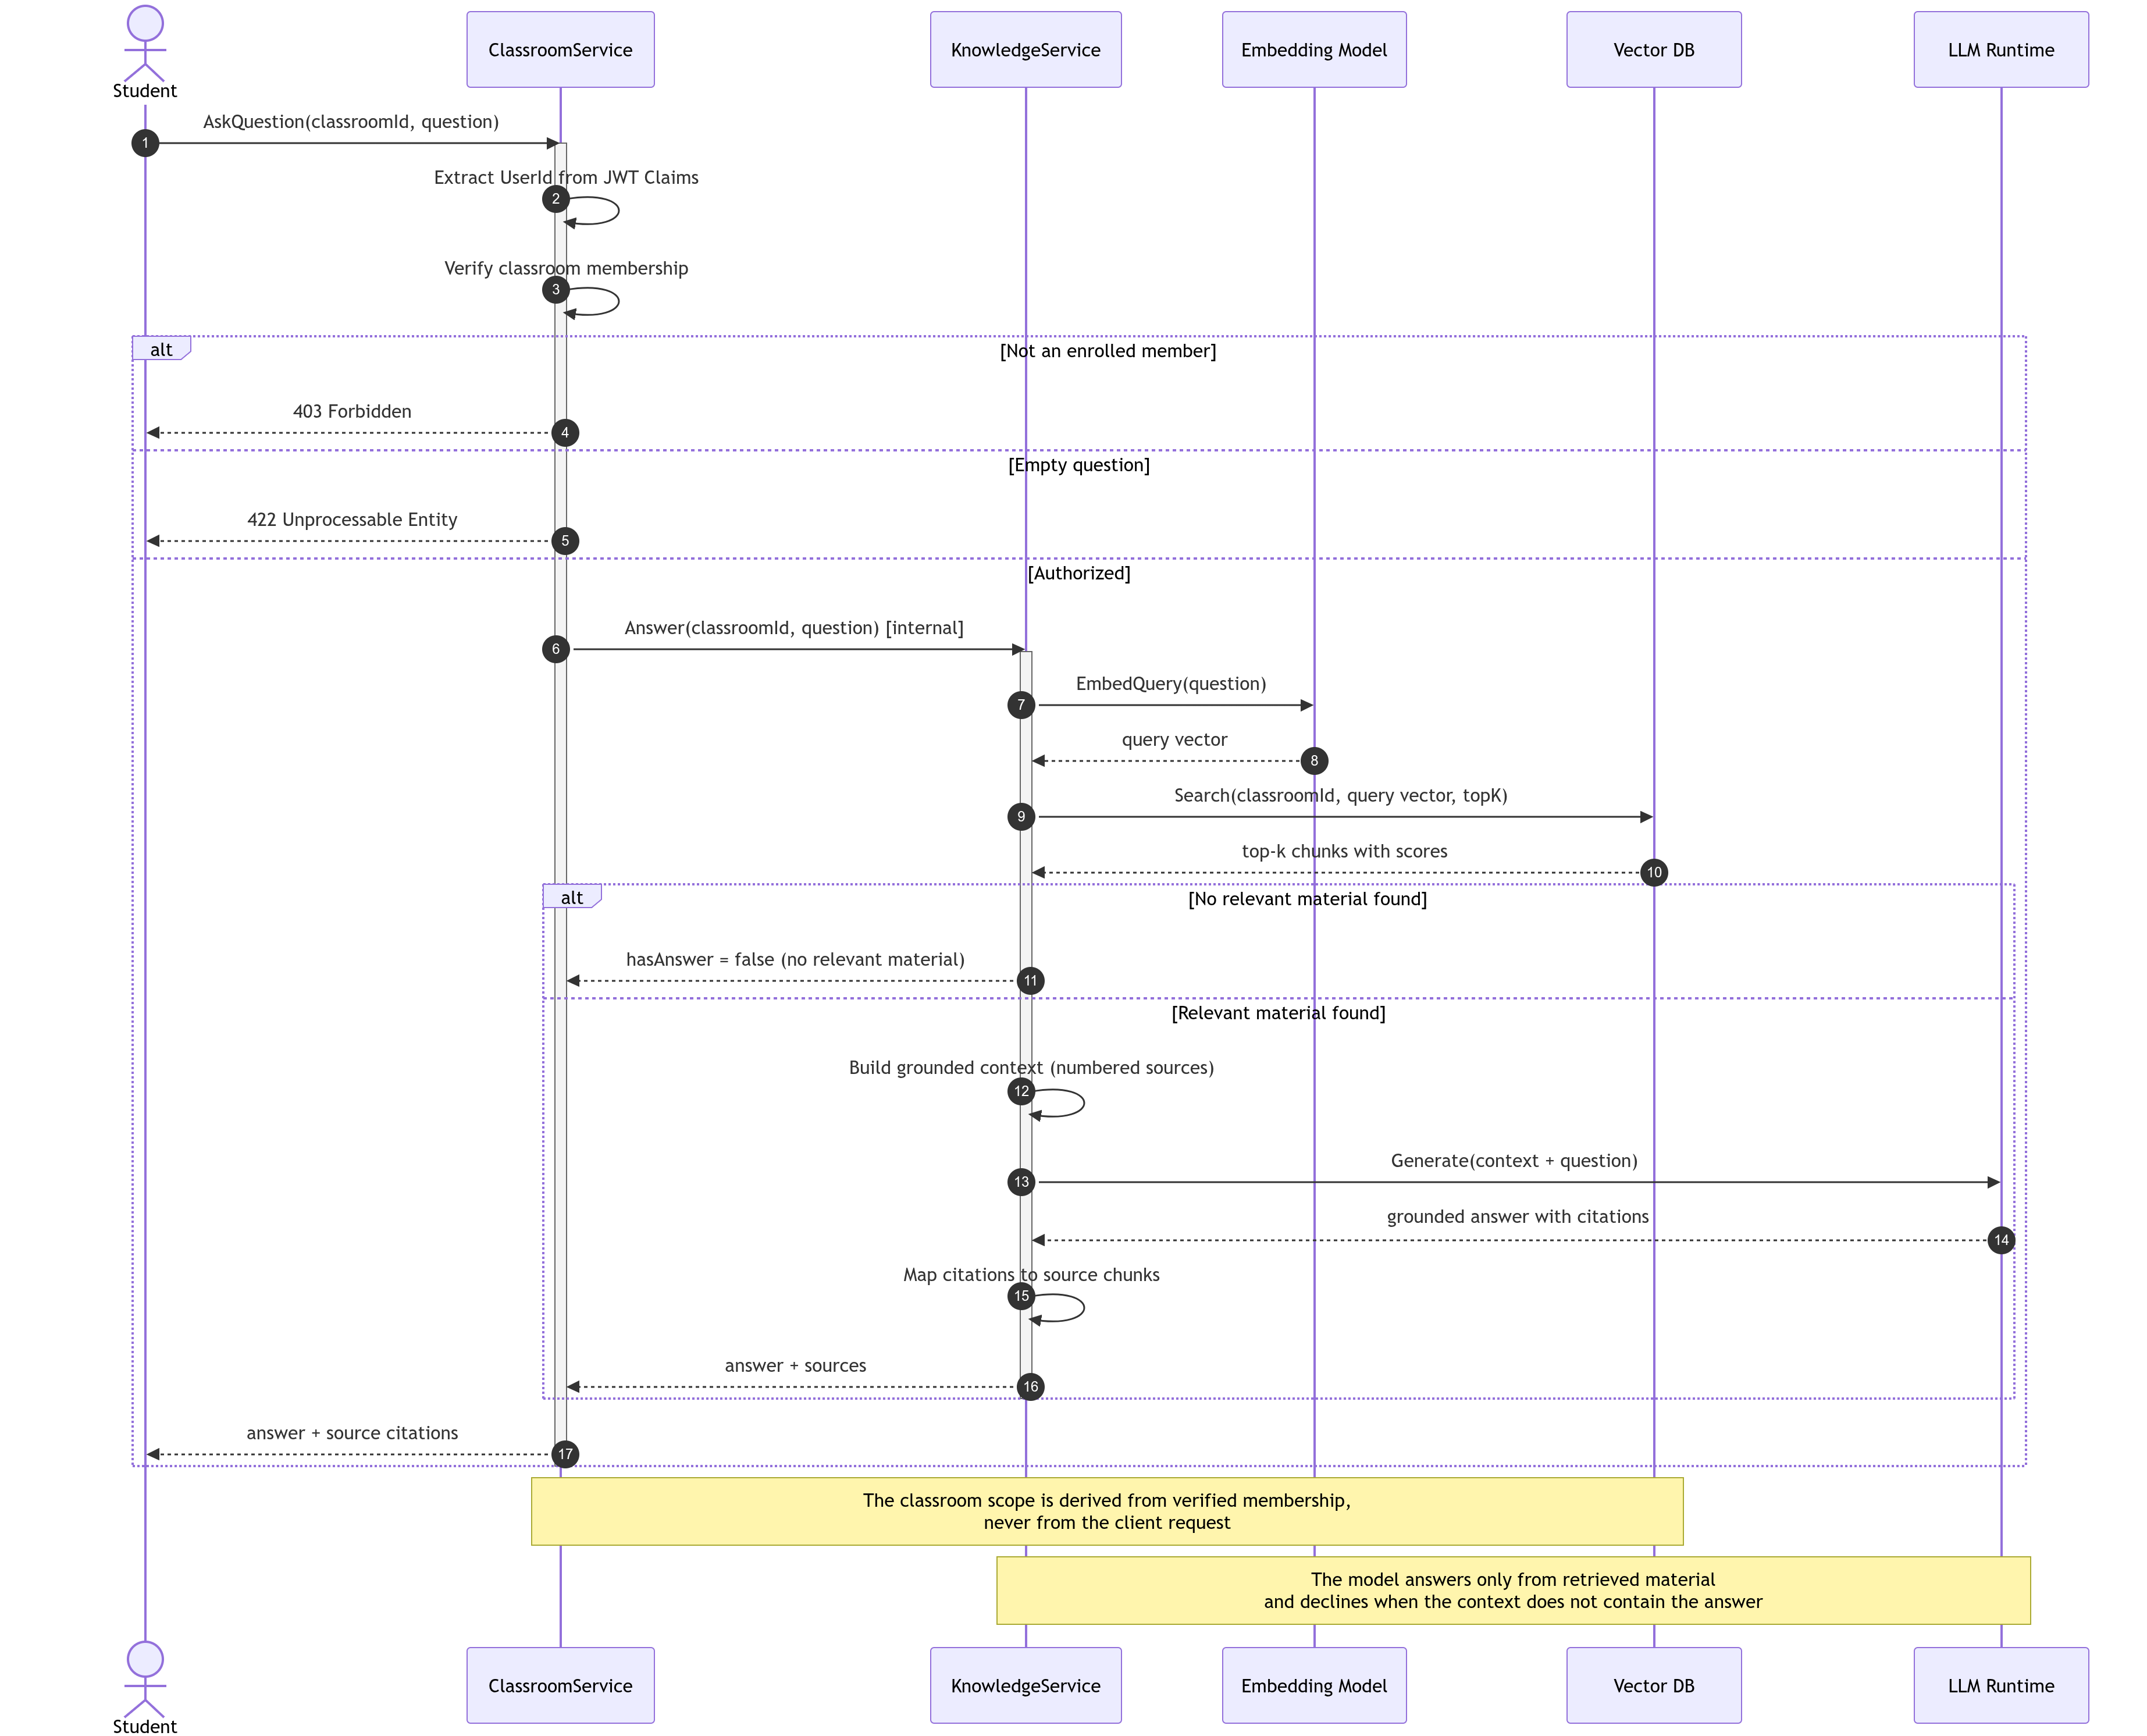
\includegraphics[width=\textwidth,height=0.8\textheight,keepaspectratio]{figures/image34.png}
  \caption{مخطط تسلسل النظام لحالة «الإجابة عن سؤال الطالب اعتمادًا على مواد الفصل»: يوضّح الرسائل المتبادلة بين الفاعل والنظام بوصفه صندوقًا أسود، أي دون إظهار الخدمات الداخلية التي تنفّذها.}
  \label{fig:image34}
\end{figure}

\subsubsection{مخطط تسلسل النظام لحالة توليد ملخّص الجلسة}

\begin{figure}[htbp]
  \centering
  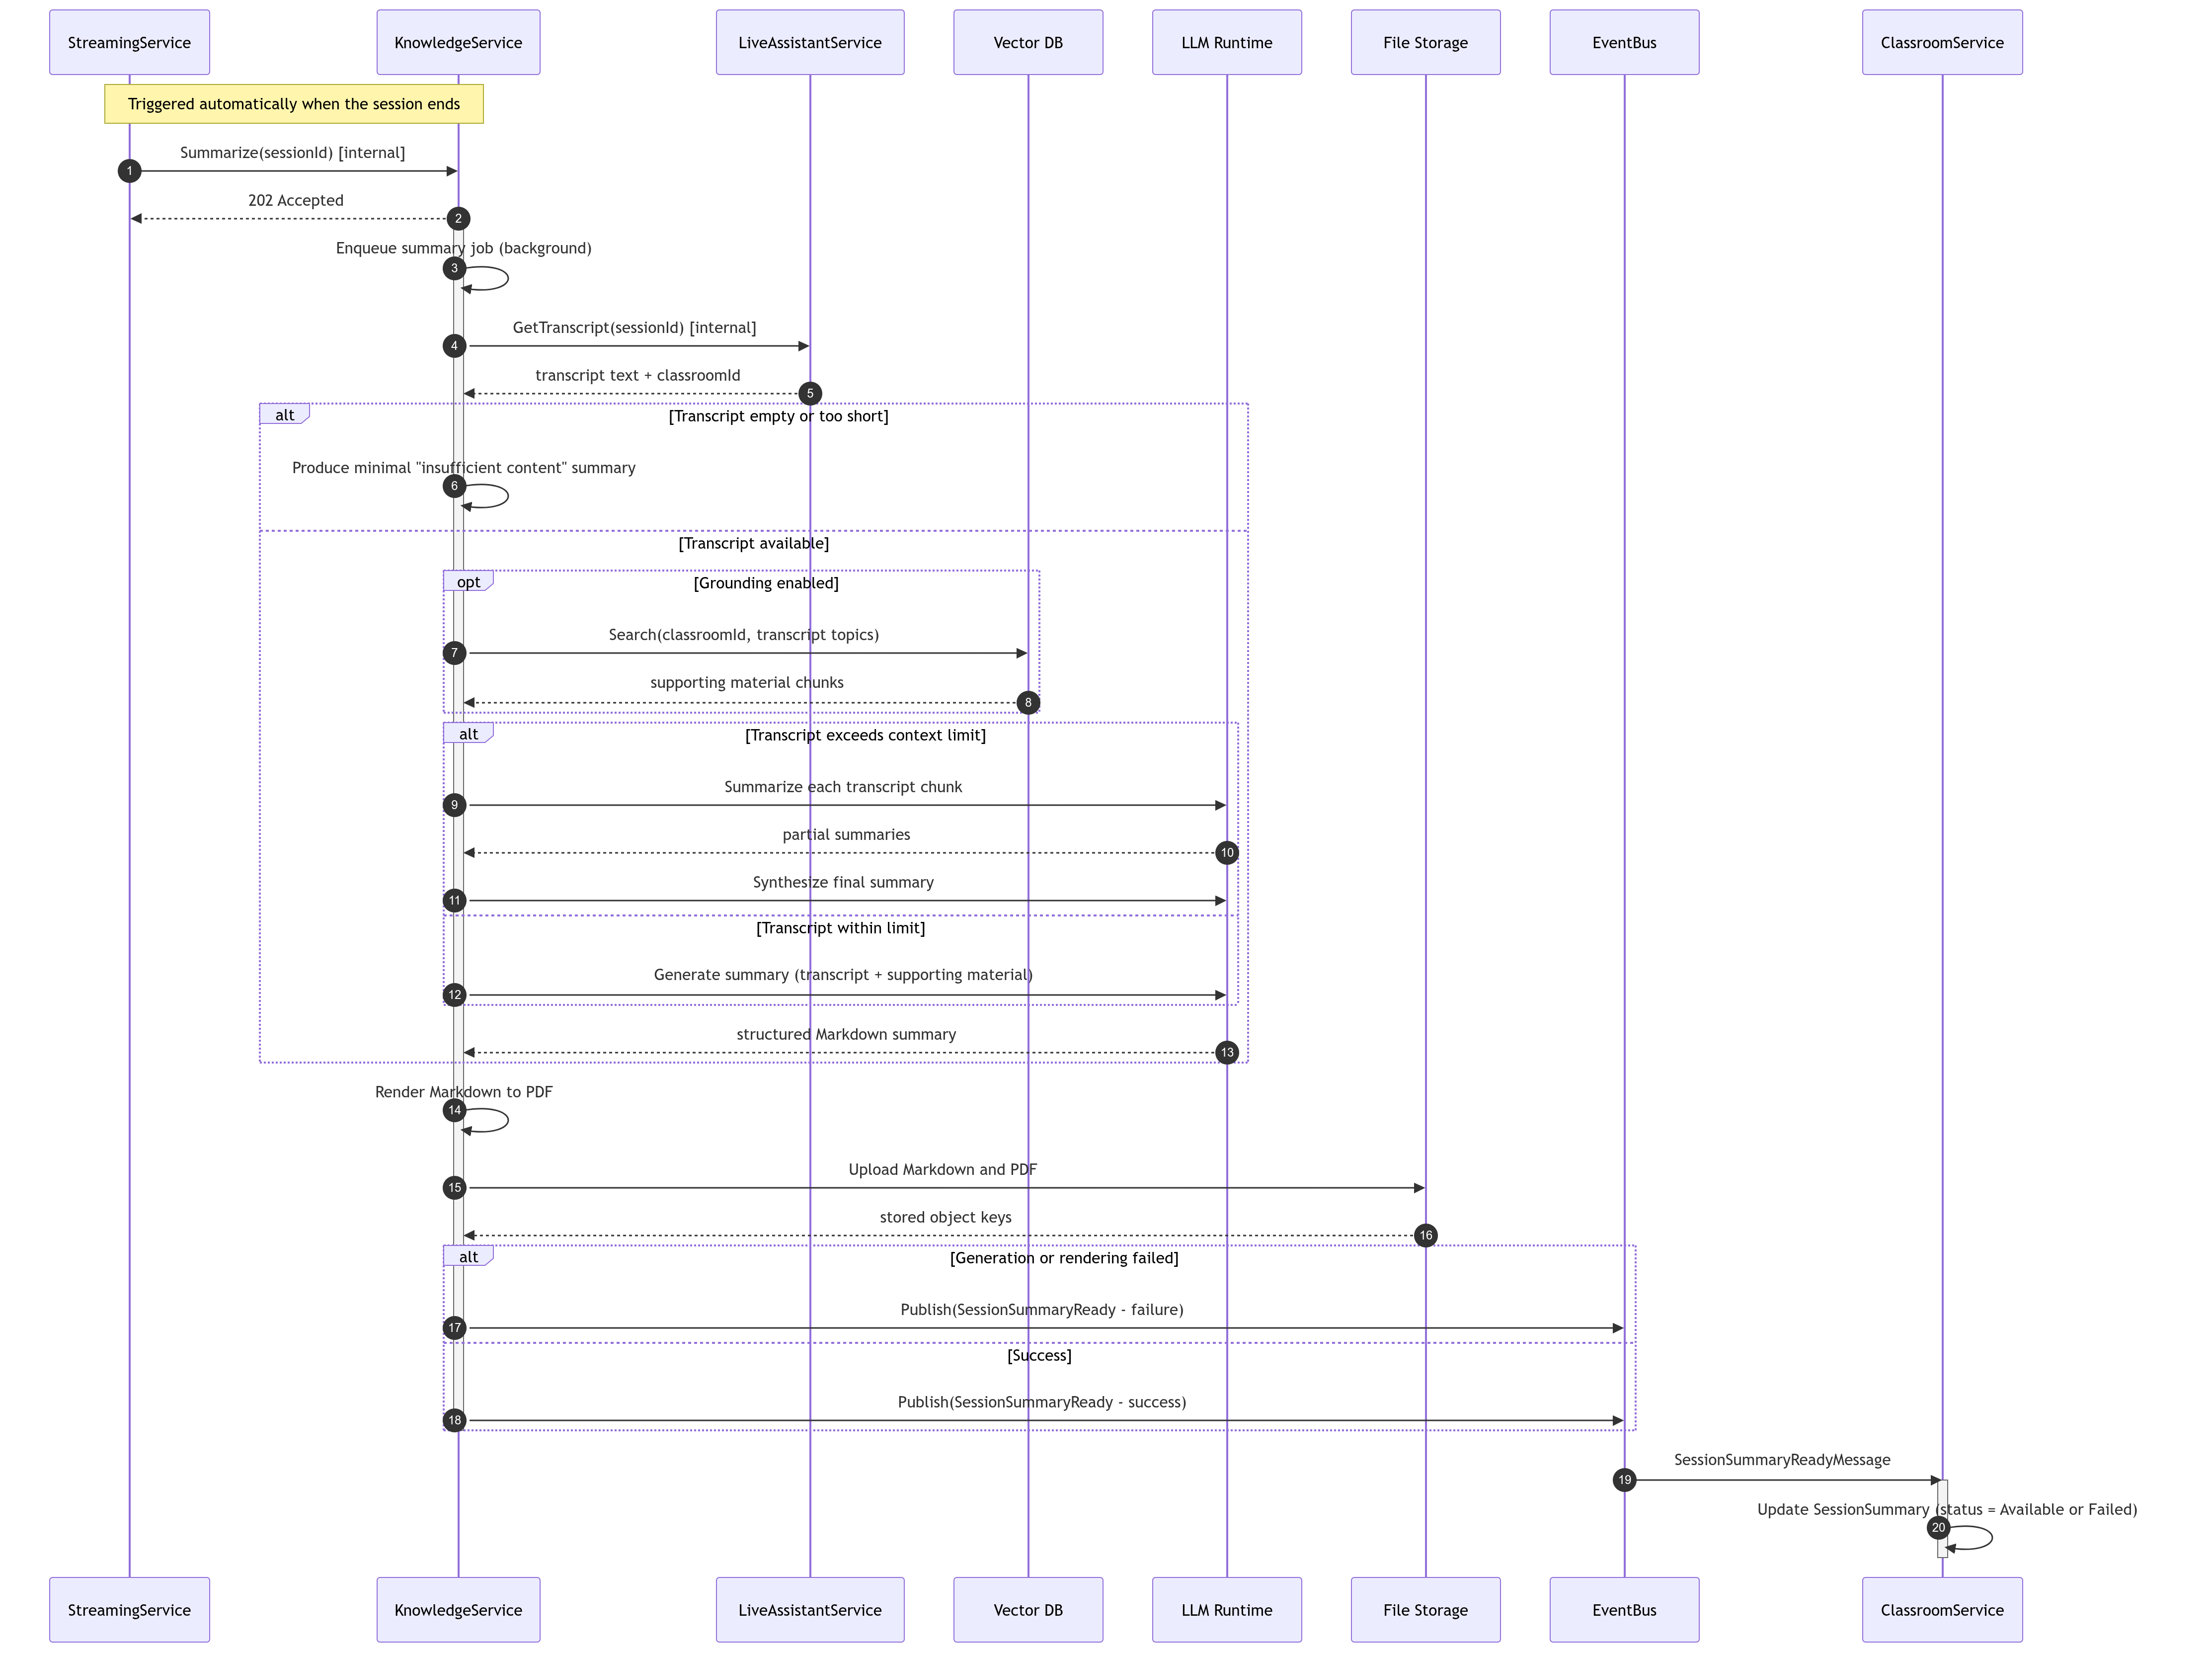
\includegraphics[width=\textwidth,height=0.8\textheight,keepaspectratio]{figures/image35.png}
  \caption{مخطط تسلسل النظام لحالة «توليد ملخّص الجلسة»: يوضّح الرسائل المتبادلة بين الفاعل والنظام بوصفه صندوقًا أسود، أي دون إظهار الخدمات الداخلية التي تنفّذها.}
  \label{fig:image35}
\end{figure}

\subsubsection{مخطط تسلسل النظام لحالة معاينة أثر حذف جلسة}

\begin{figure}[htbp]
  \centering
  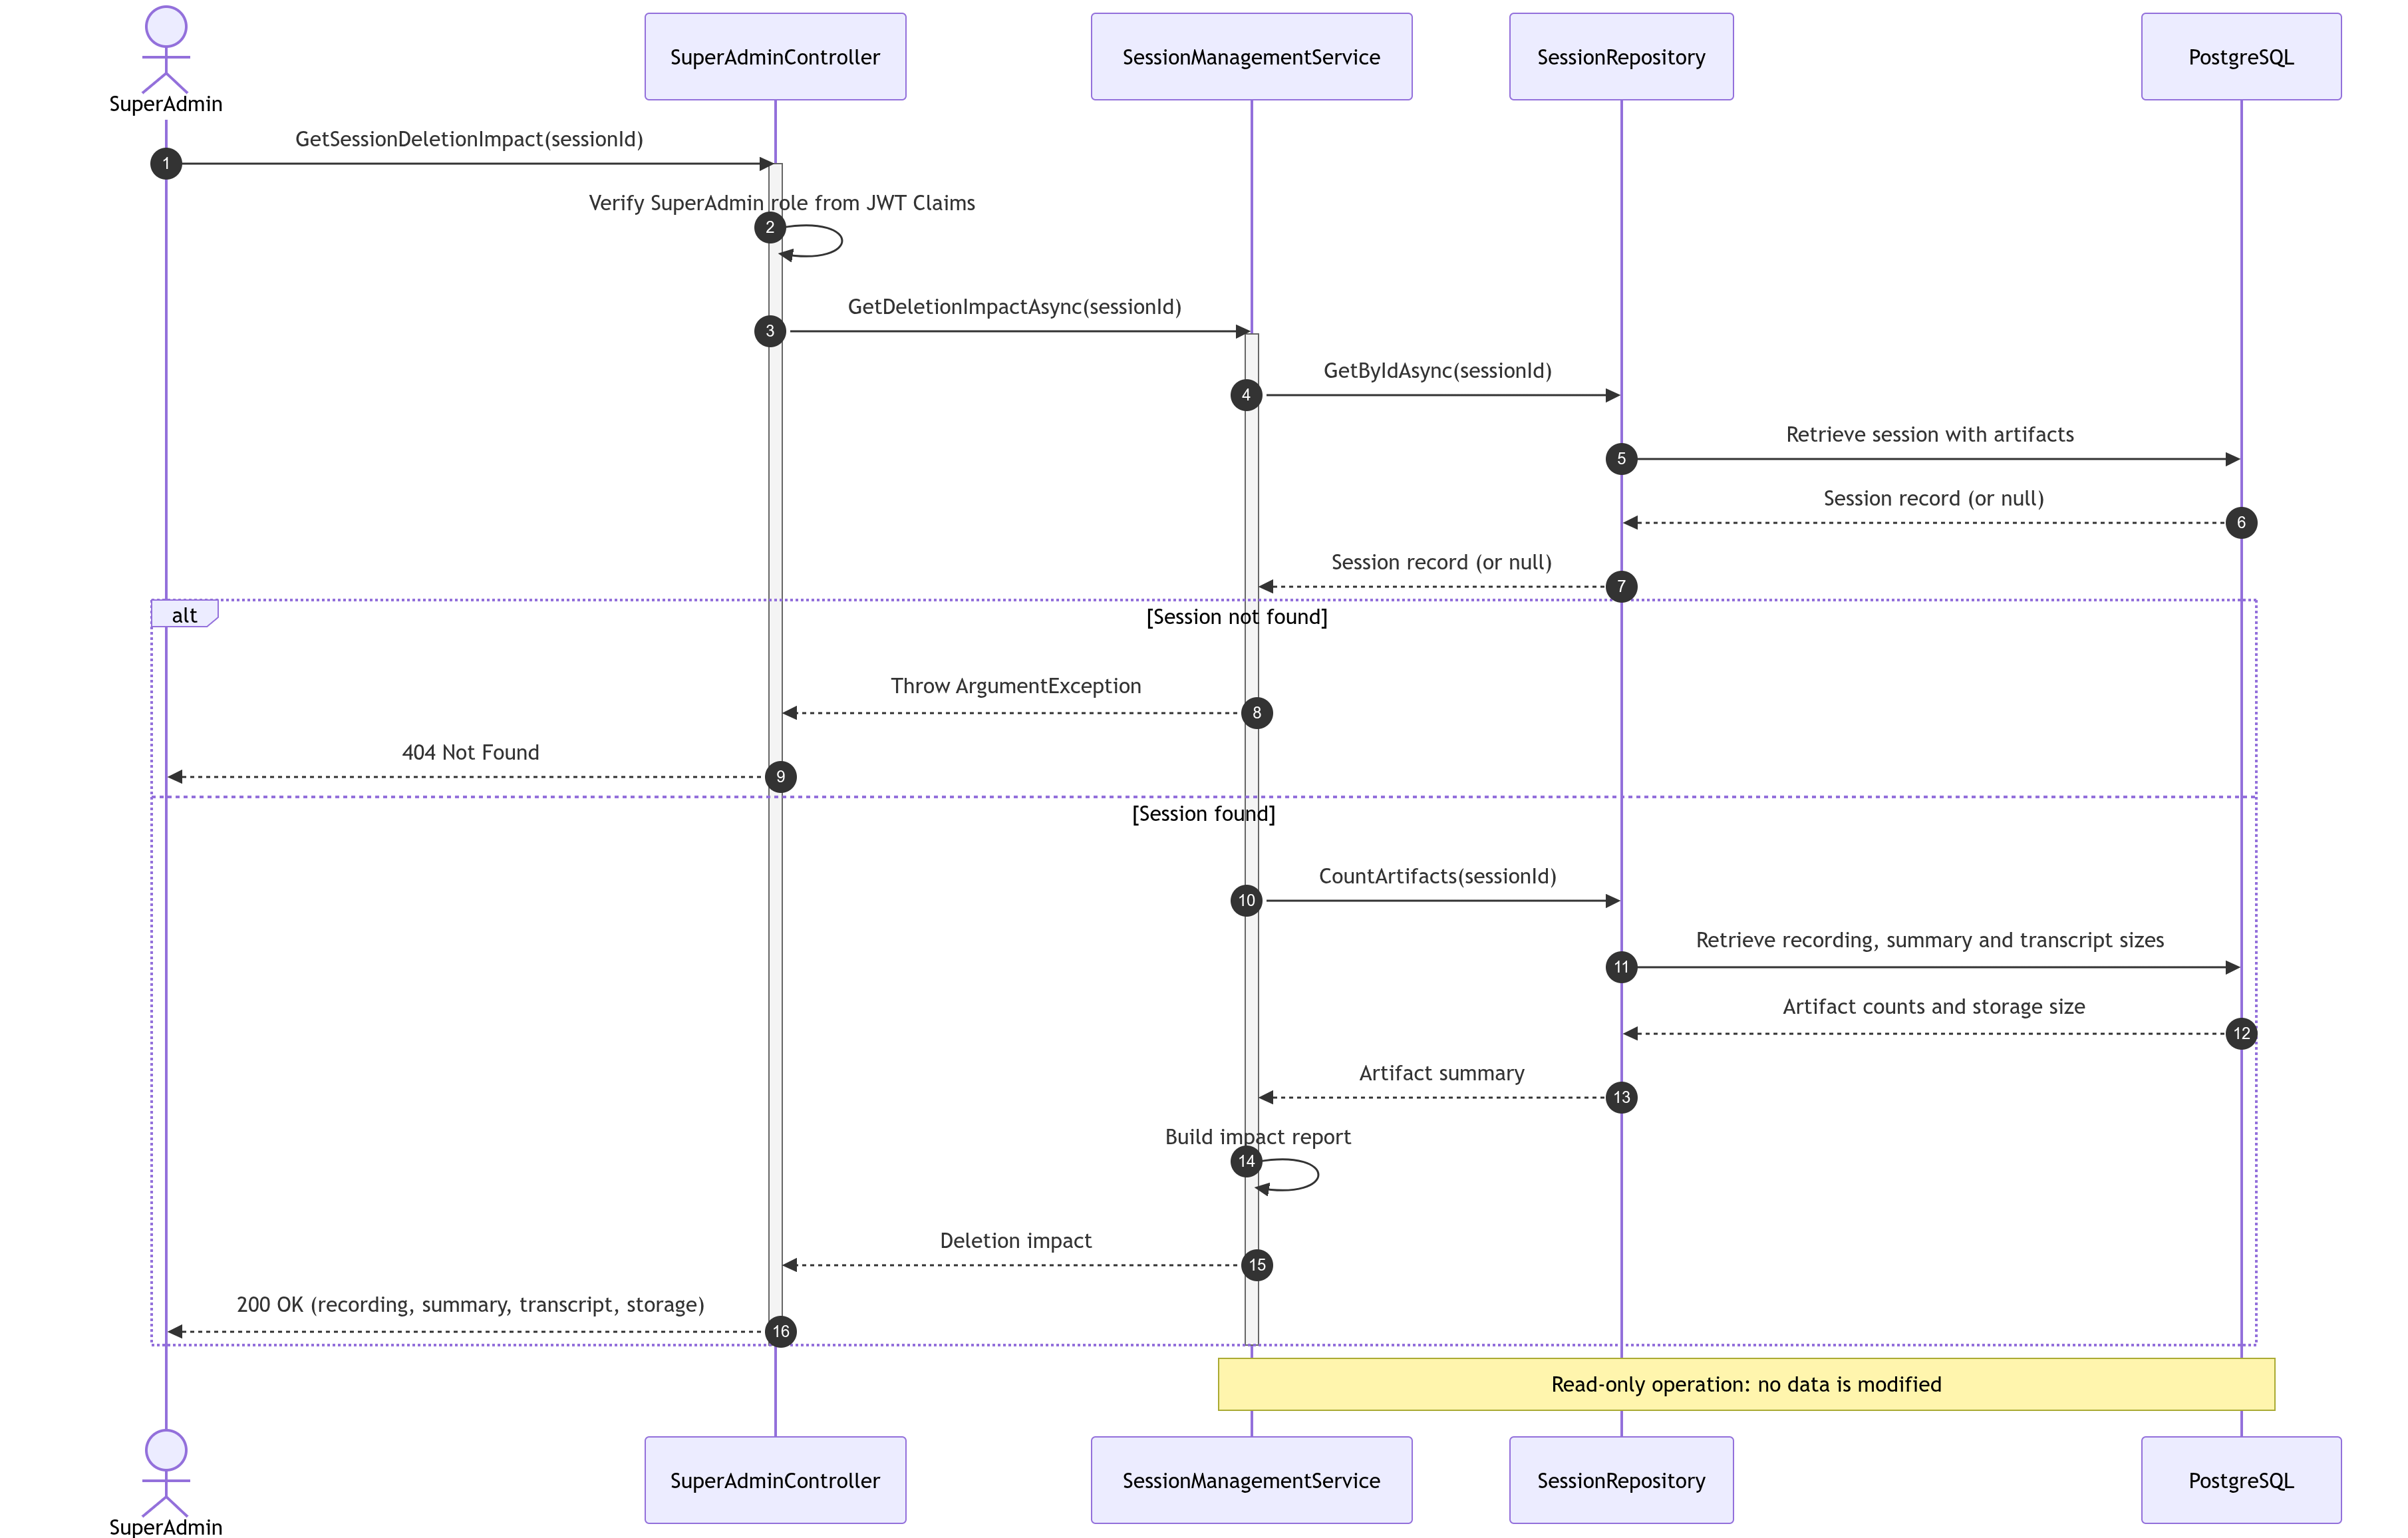
\includegraphics[width=\textwidth,height=0.8\textheight,keepaspectratio]{figures/image36.png}
  \caption{مخطط تسلسل النظام لحالة «معاينة أثر حذف جلسة»: يوضّح الرسائل المتبادلة بين الفاعل والنظام بوصفه صندوقًا أسود، أي دون إظهار الخدمات الداخلية التي تنفّذها.}
  \label{fig:image36}
\end{figure}

\subsubsection{مخطط تسلسل النظام لحالة حذف جلسة ومخرجاتها}

\begin{figure}[htbp]
  \centering
  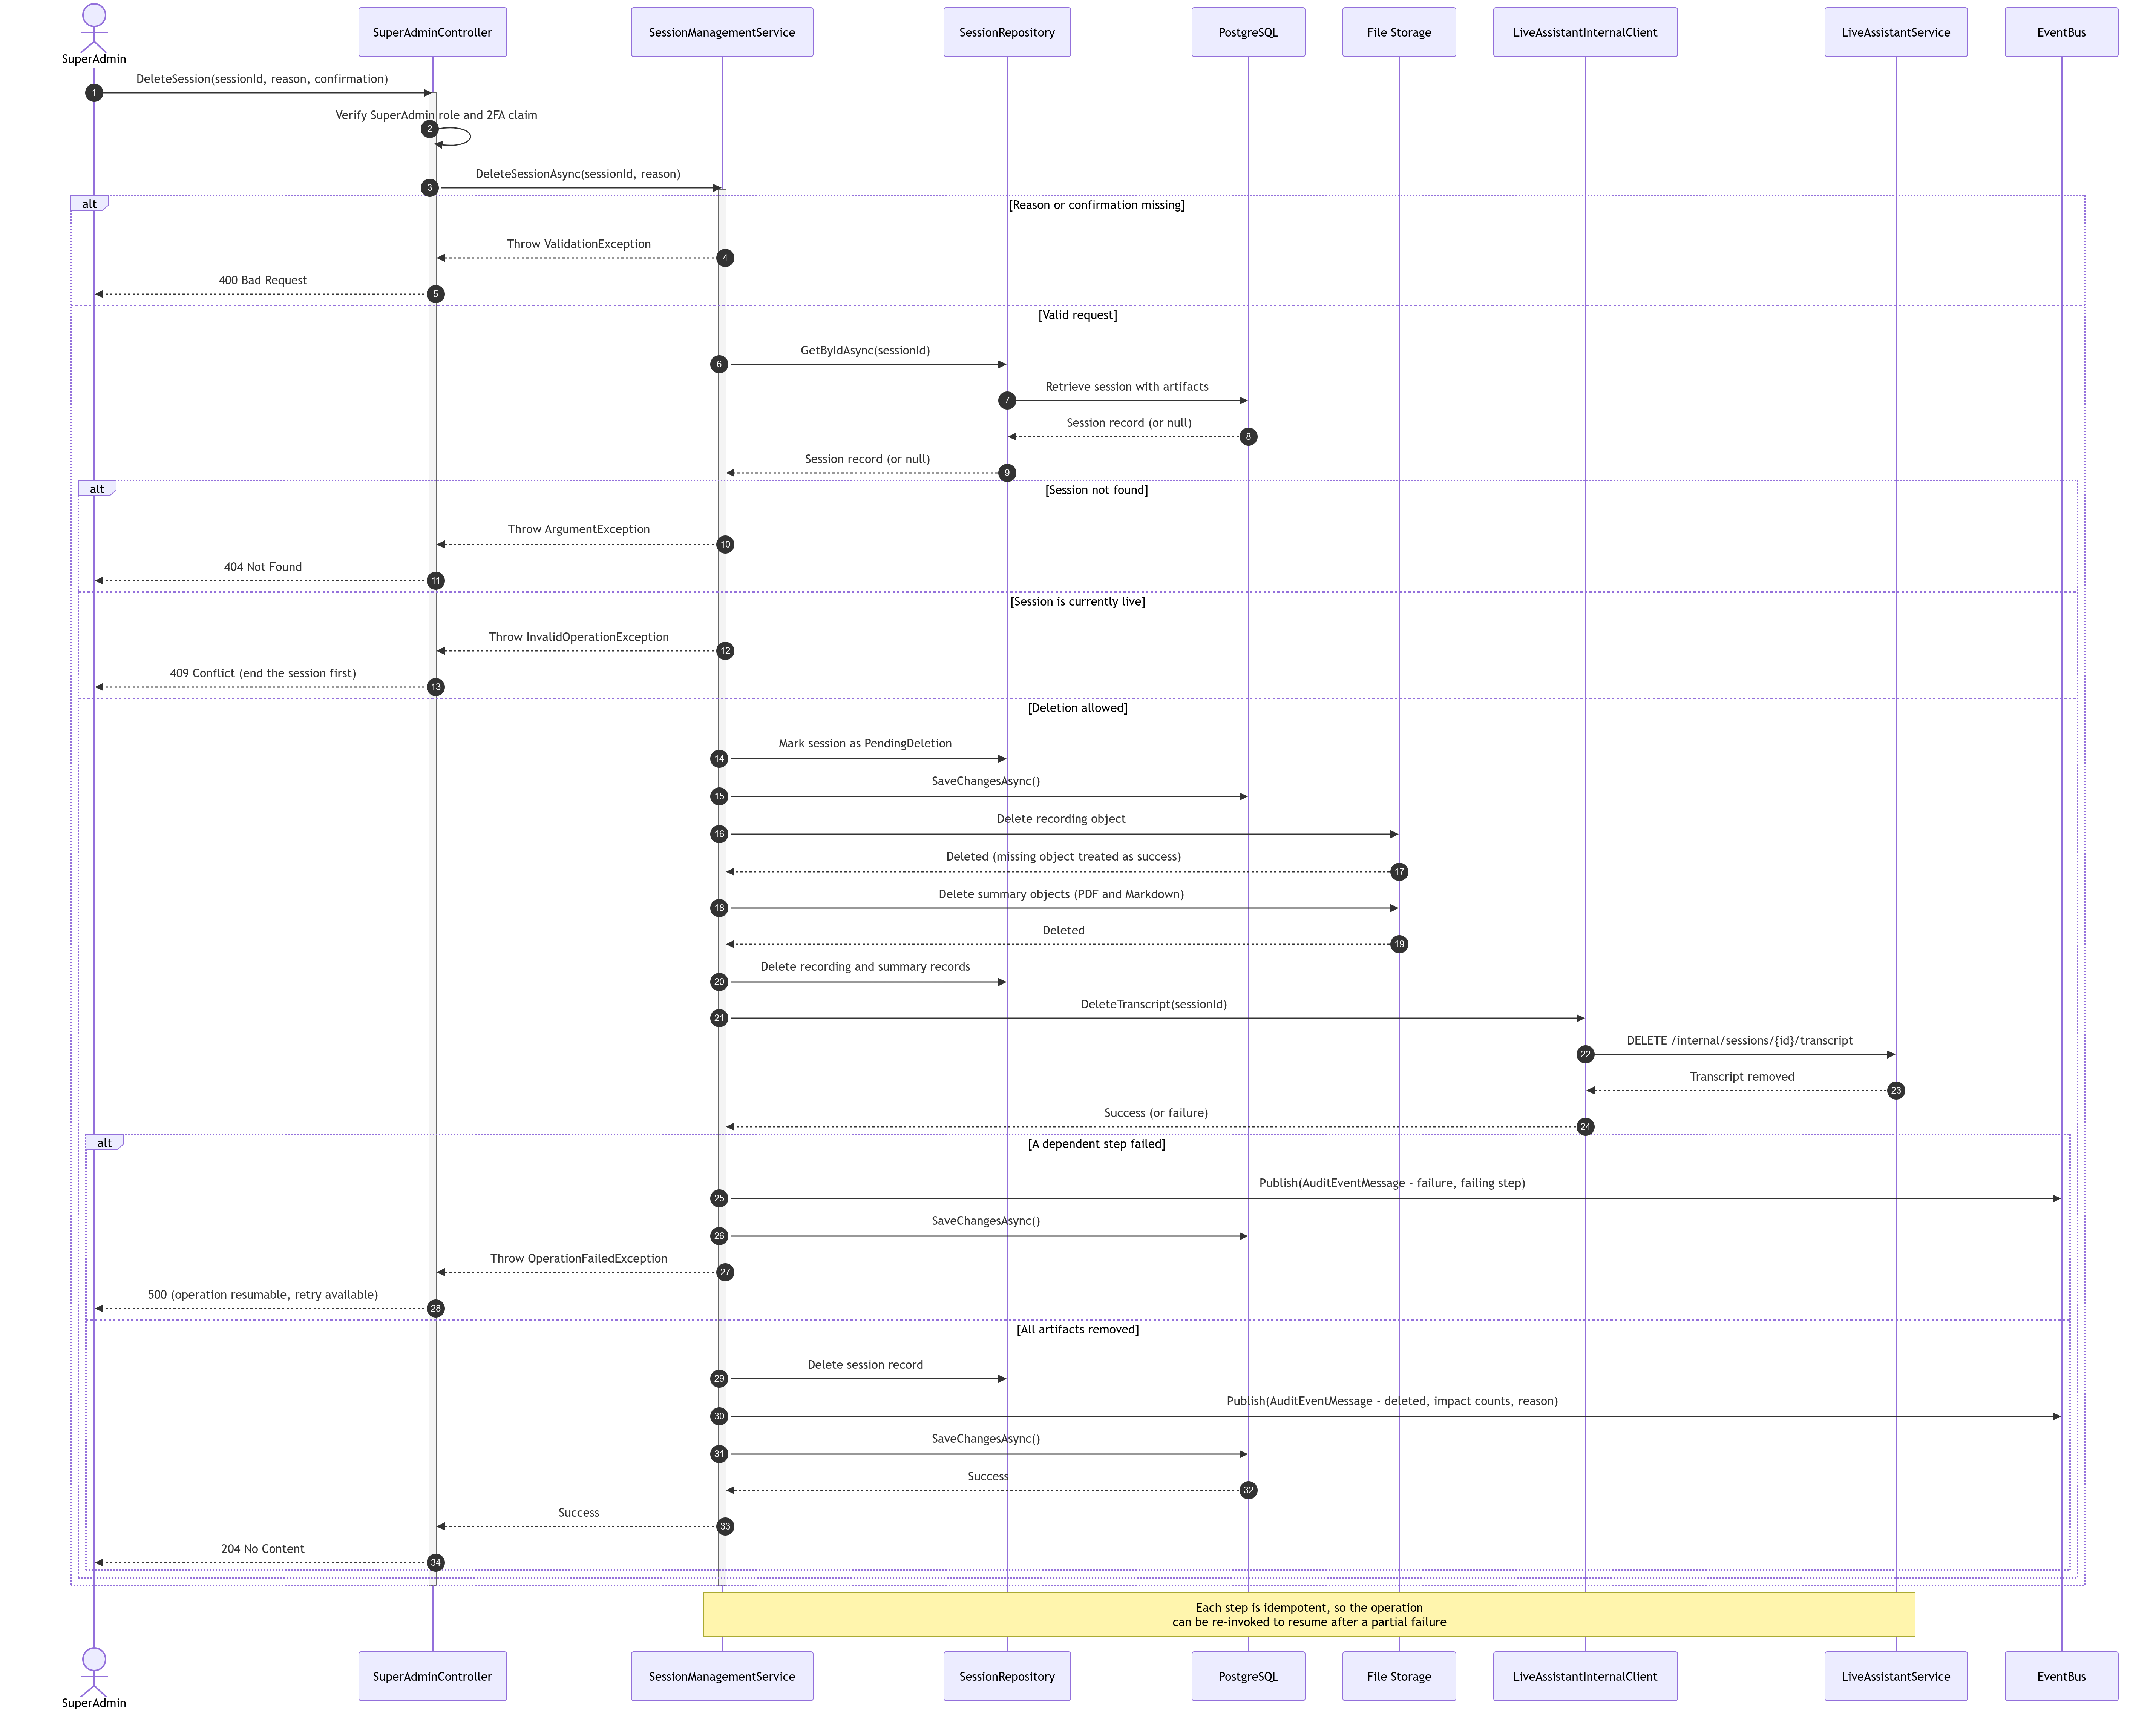
\includegraphics[width=\textwidth,height=0.8\textheight,keepaspectratio]{figures/image37.png}
  \caption{مخطط تسلسل النظام لحالة «حذف جلسة ومخرجاتها»: يوضّح الرسائل المتبادلة بين الفاعل والنظام بوصفه صندوقًا أسود، أي دون إظهار الخدمات الداخلية التي تنفّذها.}
  \label{fig:image37}
\end{figure}

\subsubsection{مخطط تسلسل النظام لحالة استعراض الملفات وحالة فهرستها}

\begin{figure}[htbp]
  \centering
  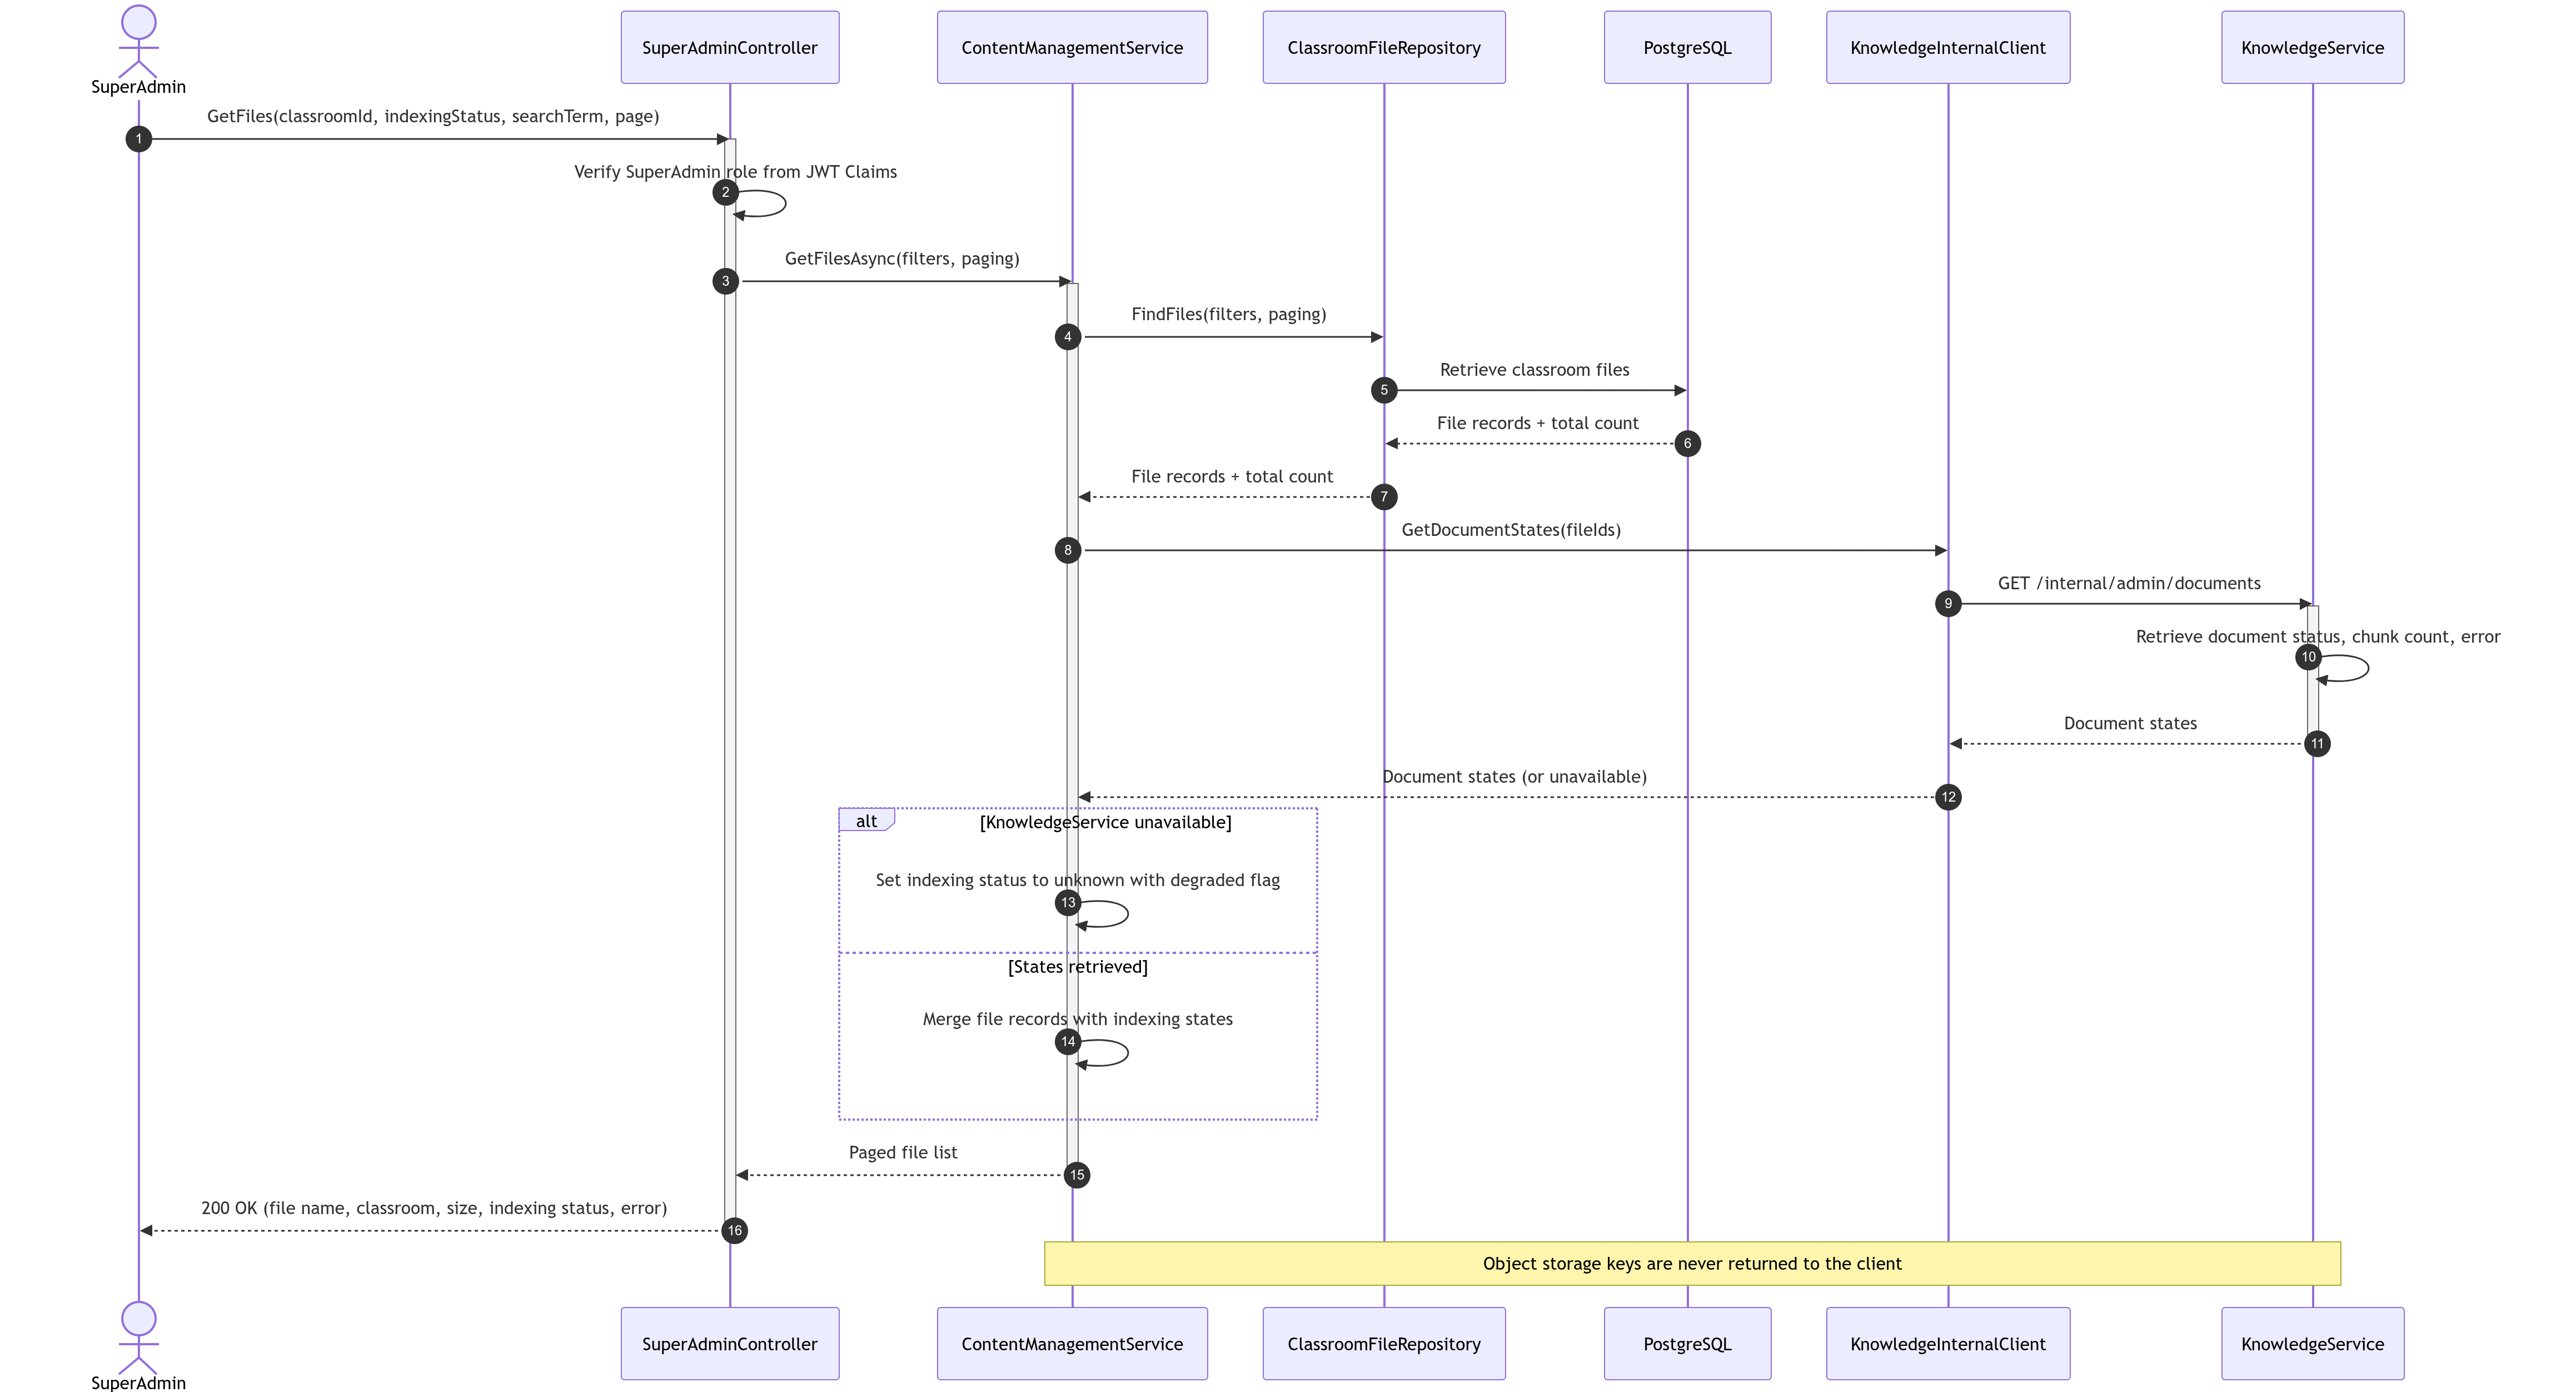
\includegraphics[width=\textwidth,height=0.8\textheight,keepaspectratio]{figures/image38.png}
  \caption{مخطط تسلسل النظام لحالة «استعراض الملفات وحالة فهرستها»: يوضّح الرسائل المتبادلة بين الفاعل والنظام بوصفه صندوقًا أسود، أي دون إظهار الخدمات الداخلية التي تنفّذها.}
  \label{fig:image38}
\end{figure}

\subsubsection{مخطط تسلسل النظام لحالة استعراض إحصائيات قاعدة المعرفة}

\begin{figure}[htbp]
  \centering
  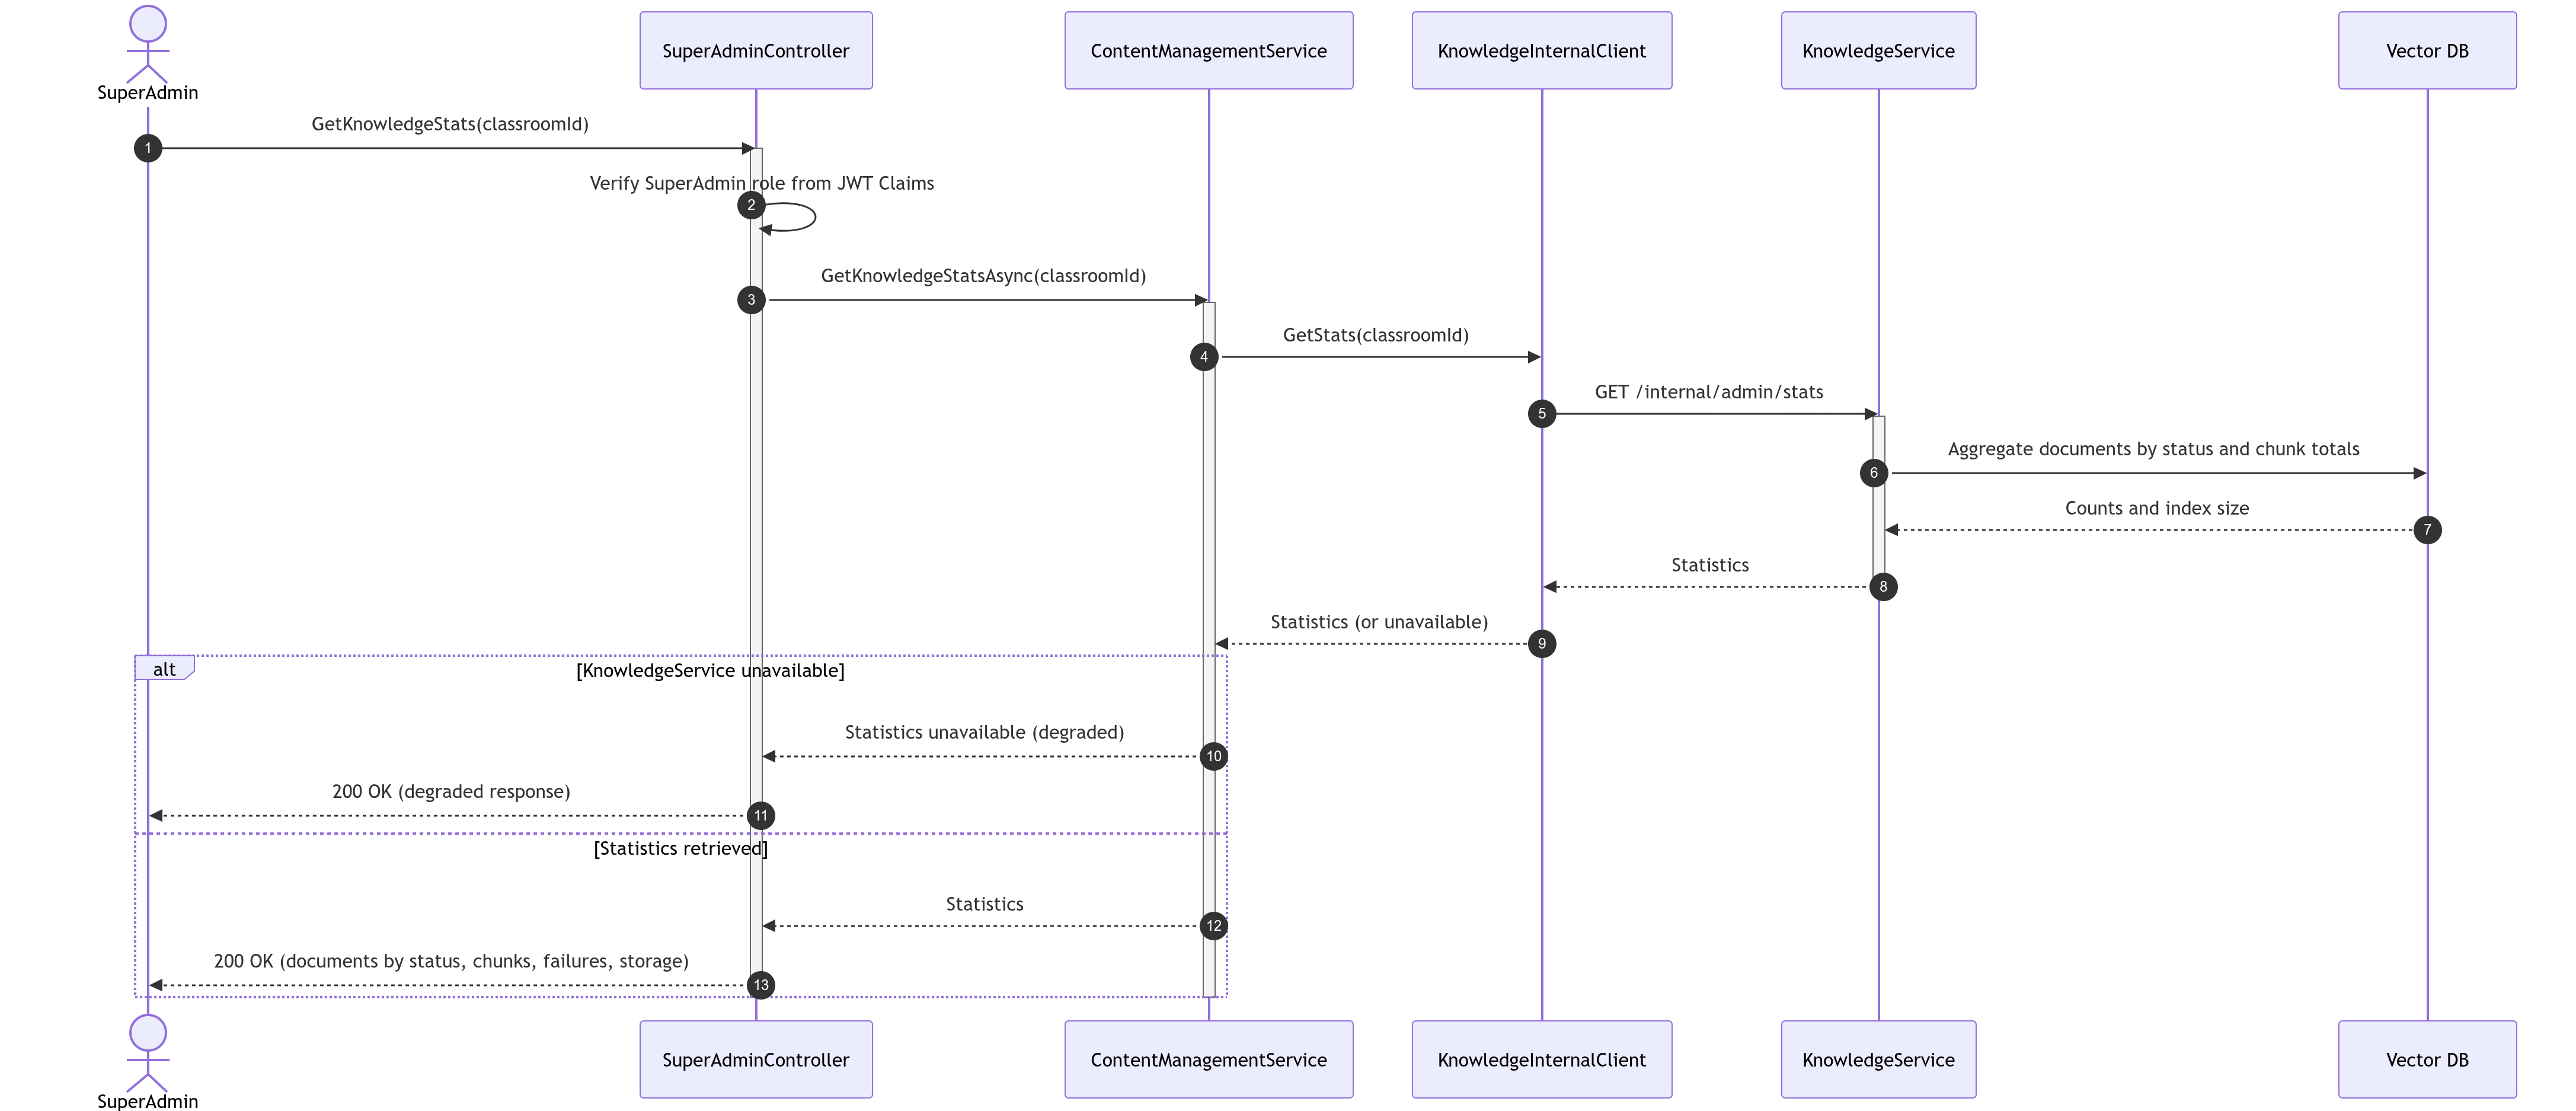
\includegraphics[width=\textwidth,height=0.8\textheight,keepaspectratio]{figures/image39.png}
  \caption{مخطط تسلسل النظام لحالة «استعراض إحصائيات قاعدة المعرفة»: يوضّح الرسائل المتبادلة بين الفاعل والنظام بوصفه صندوقًا أسود، أي دون إظهار الخدمات الداخلية التي تنفّذها.}
  \label{fig:image39}
\end{figure}

\subsubsection{مخطط تسلسل النظام لحالة إعادة فهرسة ملف أو ملفات فصل دراسي}

\begin{figure}[htbp]
  \centering
  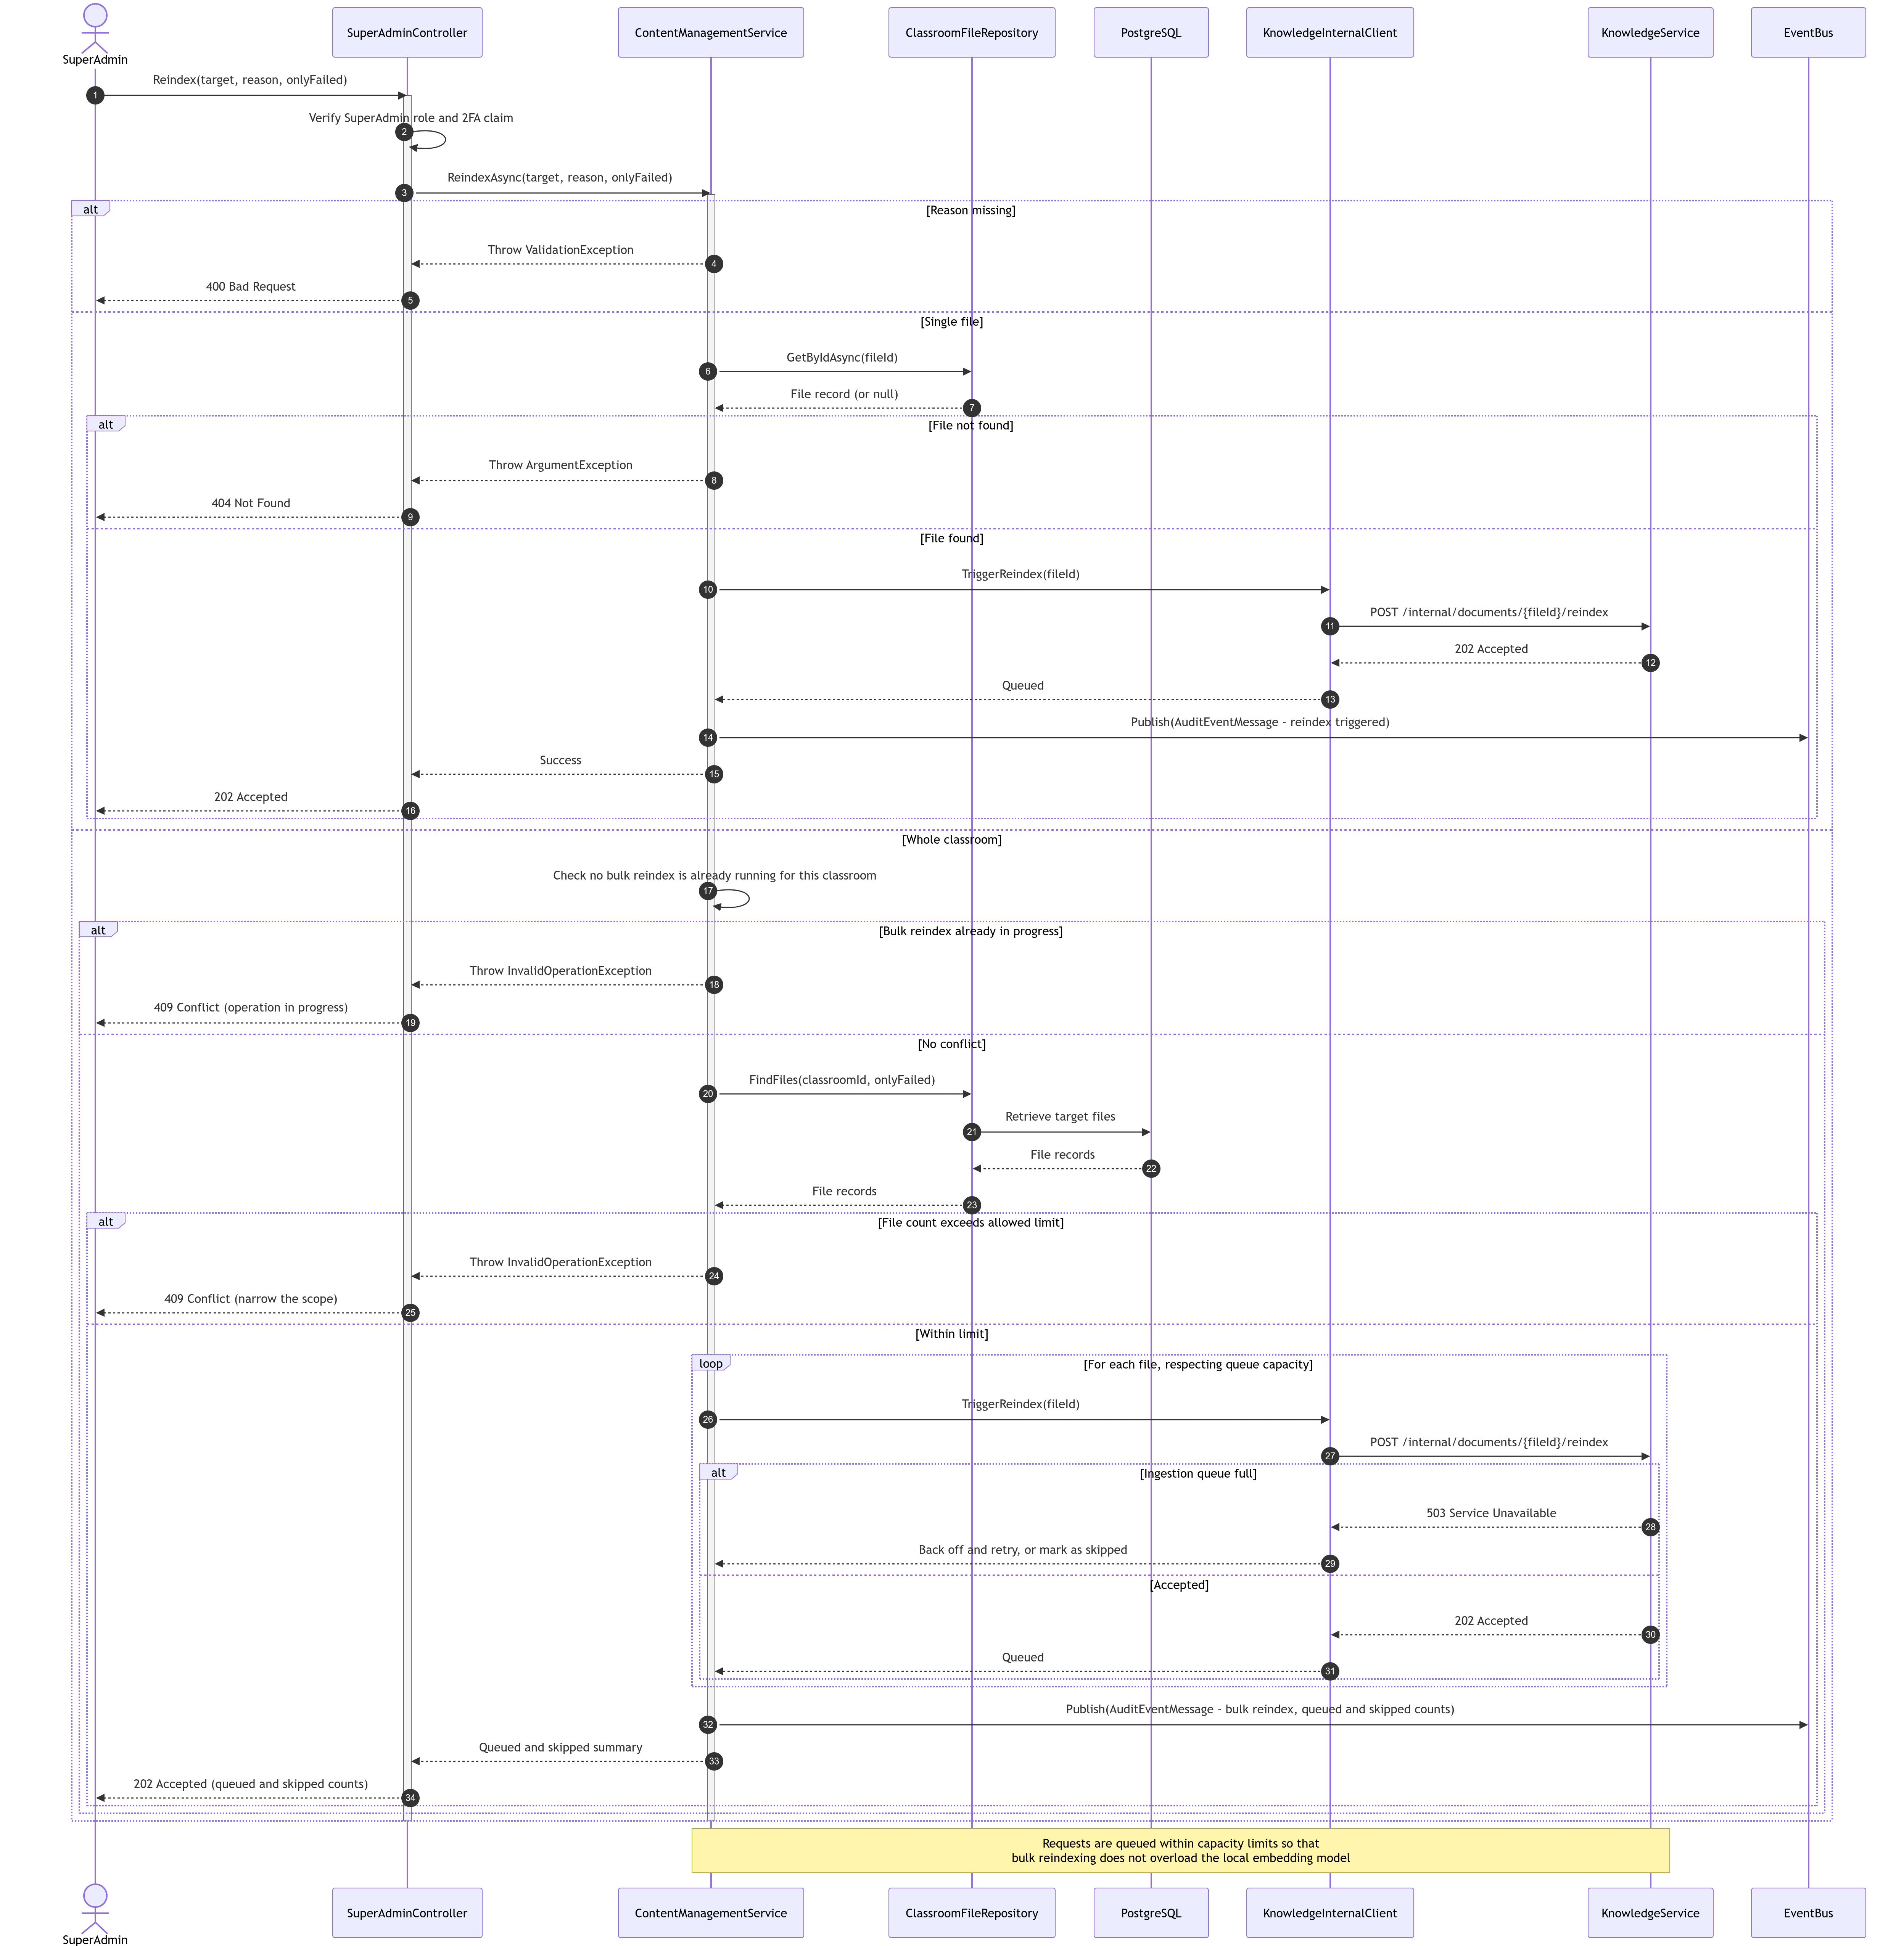
\includegraphics[width=\textwidth,height=0.8\textheight,keepaspectratio]{figures/image40.png}
  \caption{مخطط تسلسل النظام لحالة «إعادة فهرسة ملف أو ملفات فصل دراسي»: يوضّح الرسائل المتبادلة بين الفاعل والنظام بوصفه صندوقًا أسود، أي دون إظهار الخدمات الداخلية التي تنفّذها.}
  \label{fig:image40}
\end{figure}

\subsubsection{مخطط تسلسل النظام لحالة حذف ملف مع مقاطعه المفهرسة}

\begin{figure}[htbp]
  \centering
  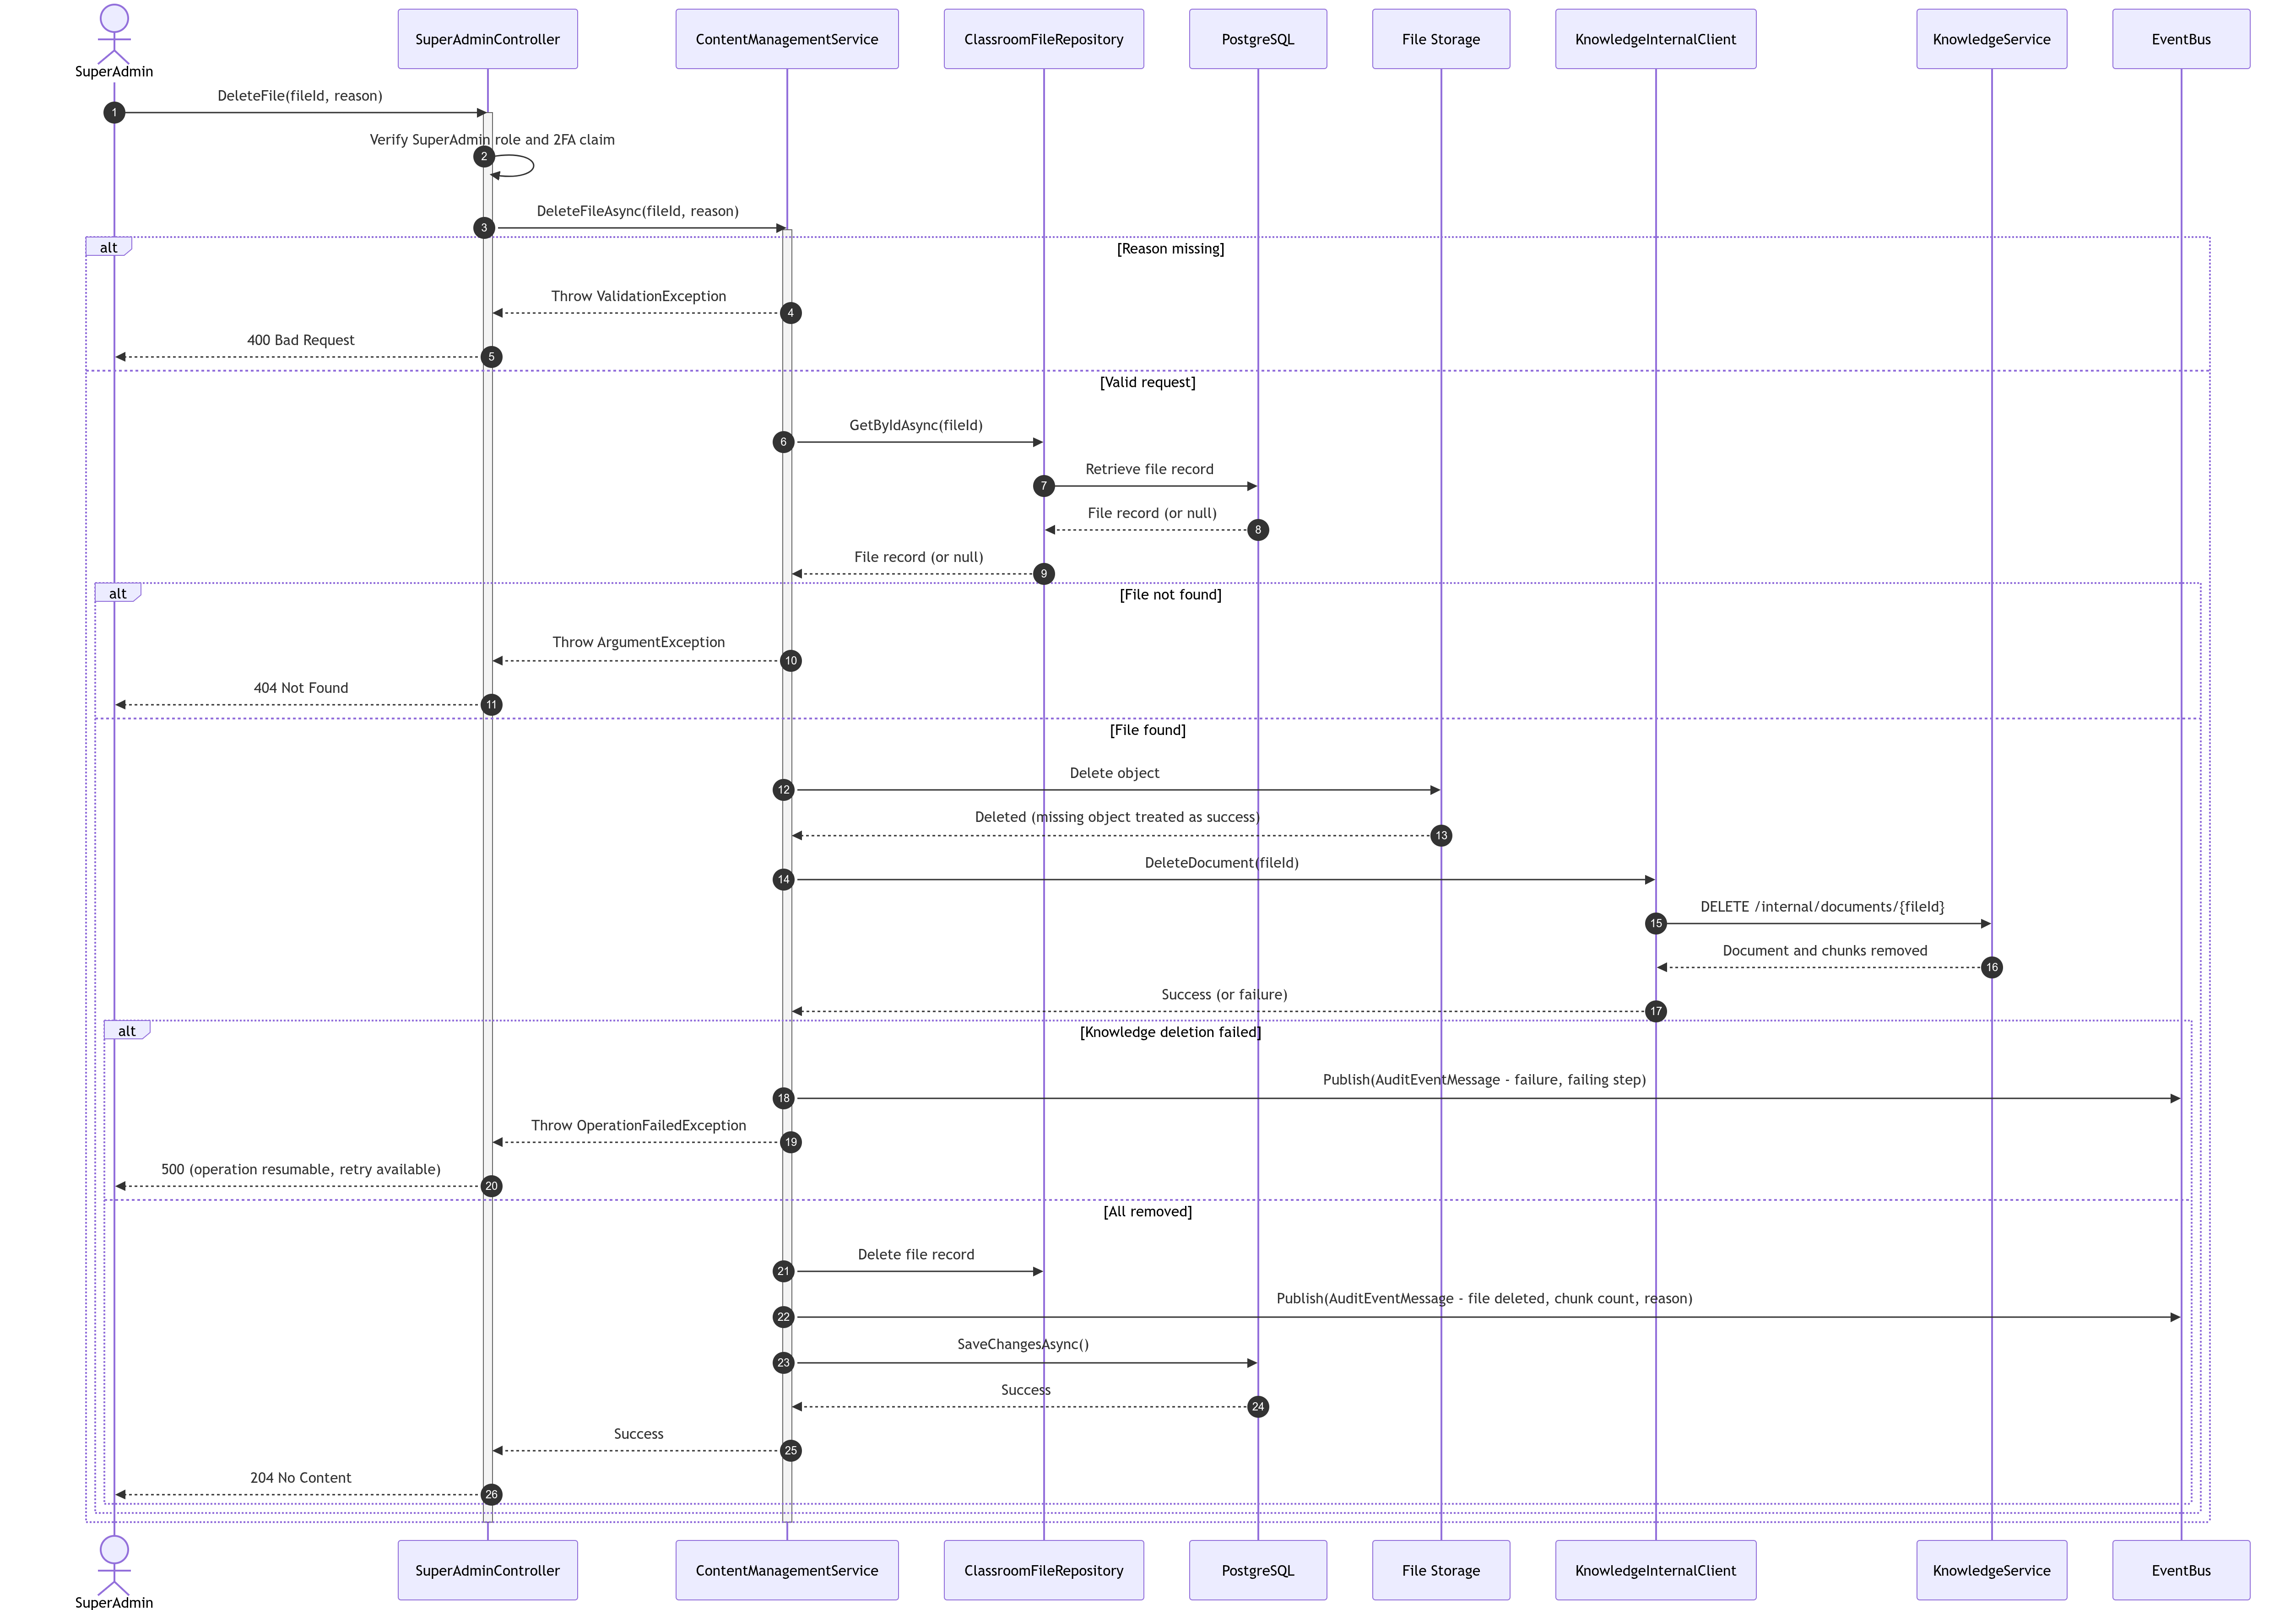
\includegraphics[width=\textwidth,height=0.8\textheight,keepaspectratio]{figures/image41.png}
  \caption{مخطط تسلسل النظام لحالة «حذف ملف مع مقاطعه المفهرسة»: يوضّح الرسائل المتبادلة بين الفاعل والنظام بوصفه صندوقًا أسود، أي دون إظهار الخدمات الداخلية التي تنفّذها.}
  \label{fig:image41}
\end{figure}

\subsubsection{مخطط تسلسل النظام لحالة استعراض التسجيلات والملخصات وحالاتها}

\begin{figure}[htbp]
  \centering
  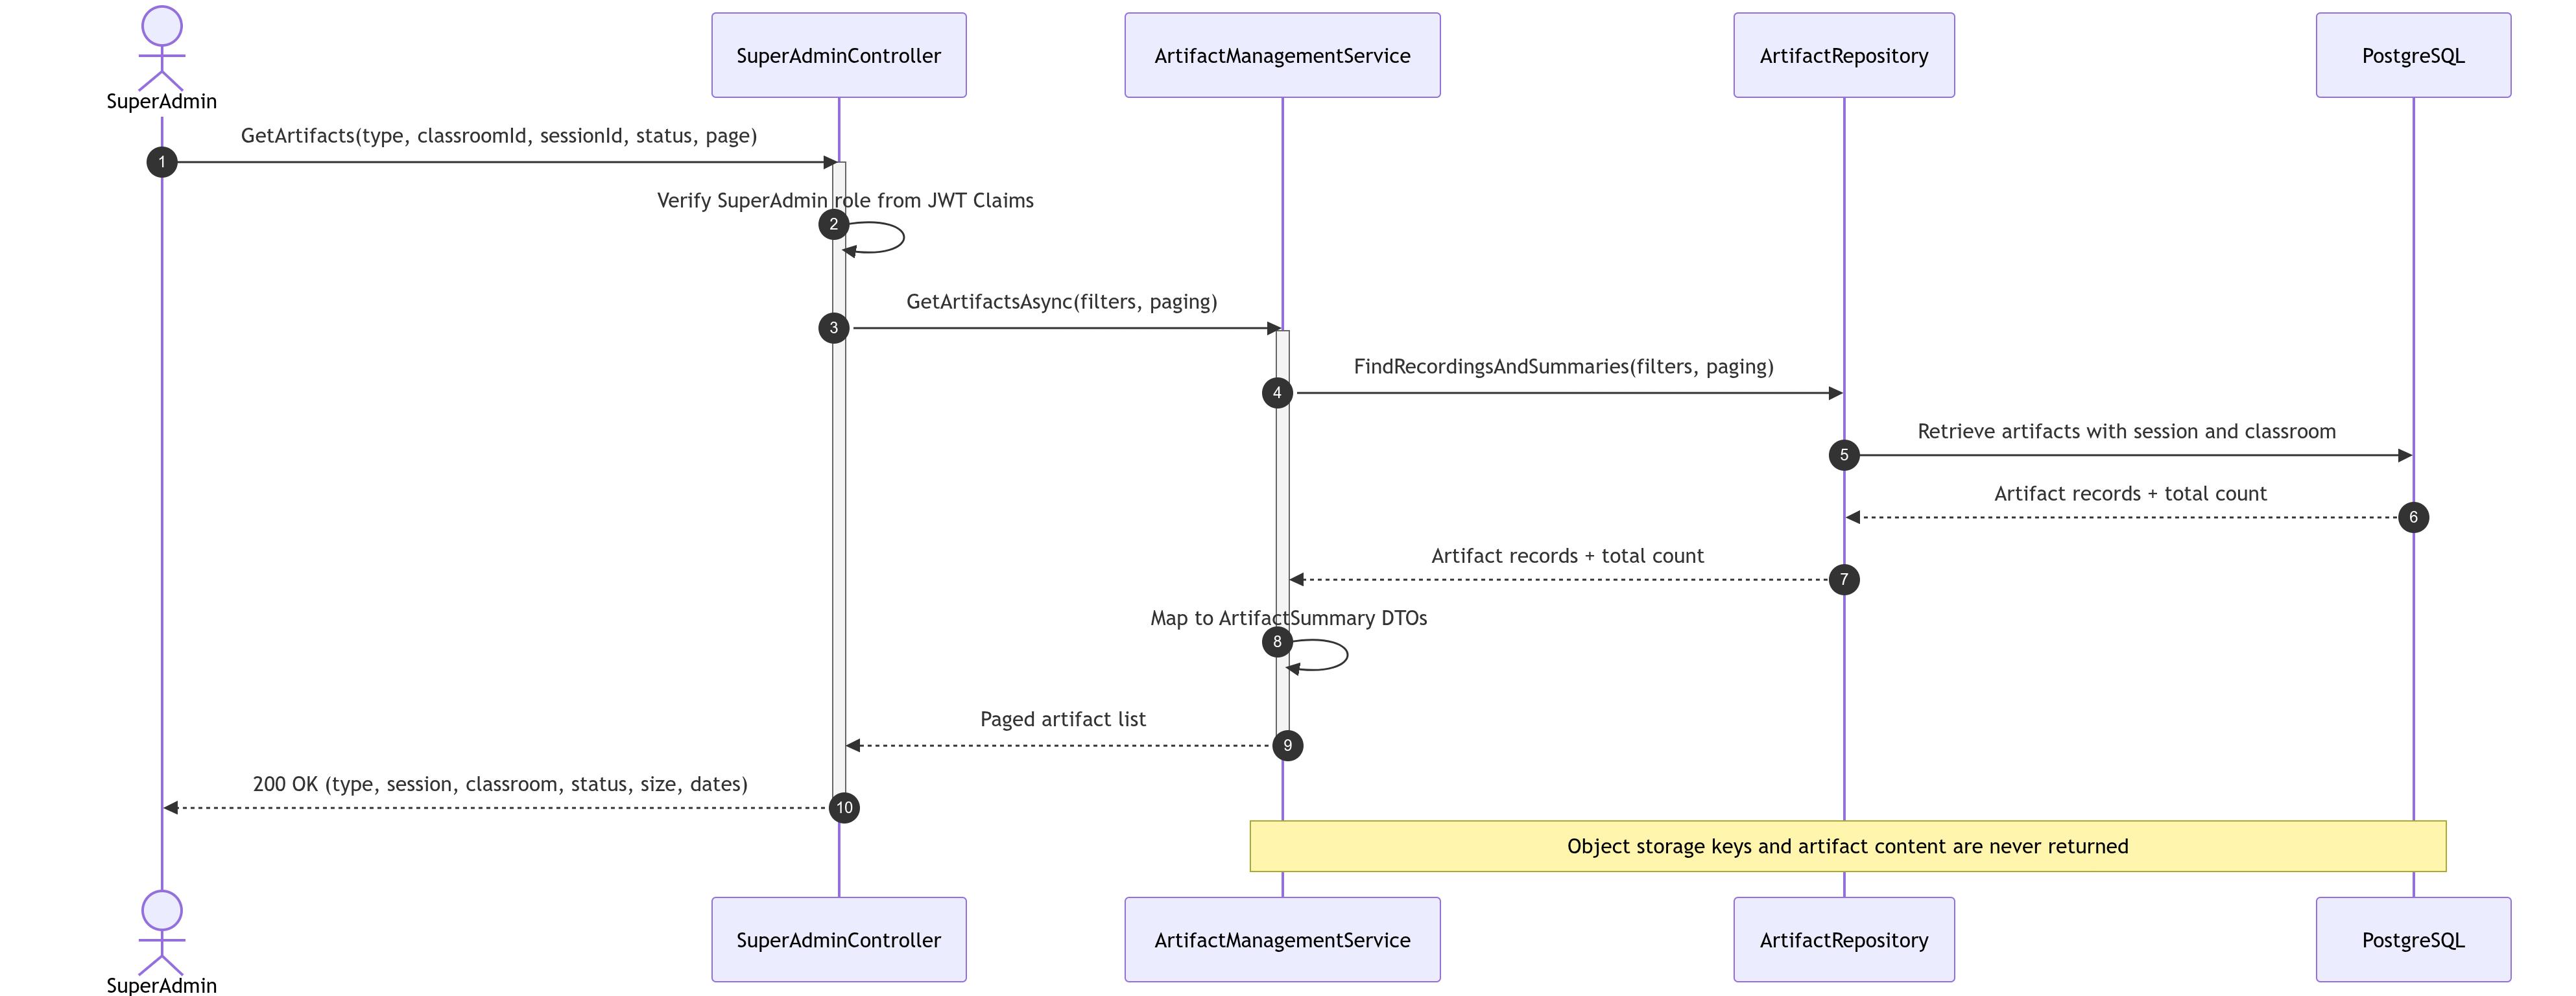
\includegraphics[width=\textwidth,height=0.8\textheight,keepaspectratio]{figures/image42.png}
  \caption{مخطط تسلسل النظام لحالة «استعراض التسجيلات والملخصات وحالاتها»: يوضّح الرسائل المتبادلة بين الفاعل والنظام بوصفه صندوقًا أسود، أي دون إظهار الخدمات الداخلية التي تنفّذها.}
  \label{fig:image42}
\end{figure}

\subsubsection{مخطط تسلسل النظام لحالة حذف تسجيل أو ملخص}

\begin{figure}[htbp]
  \centering
  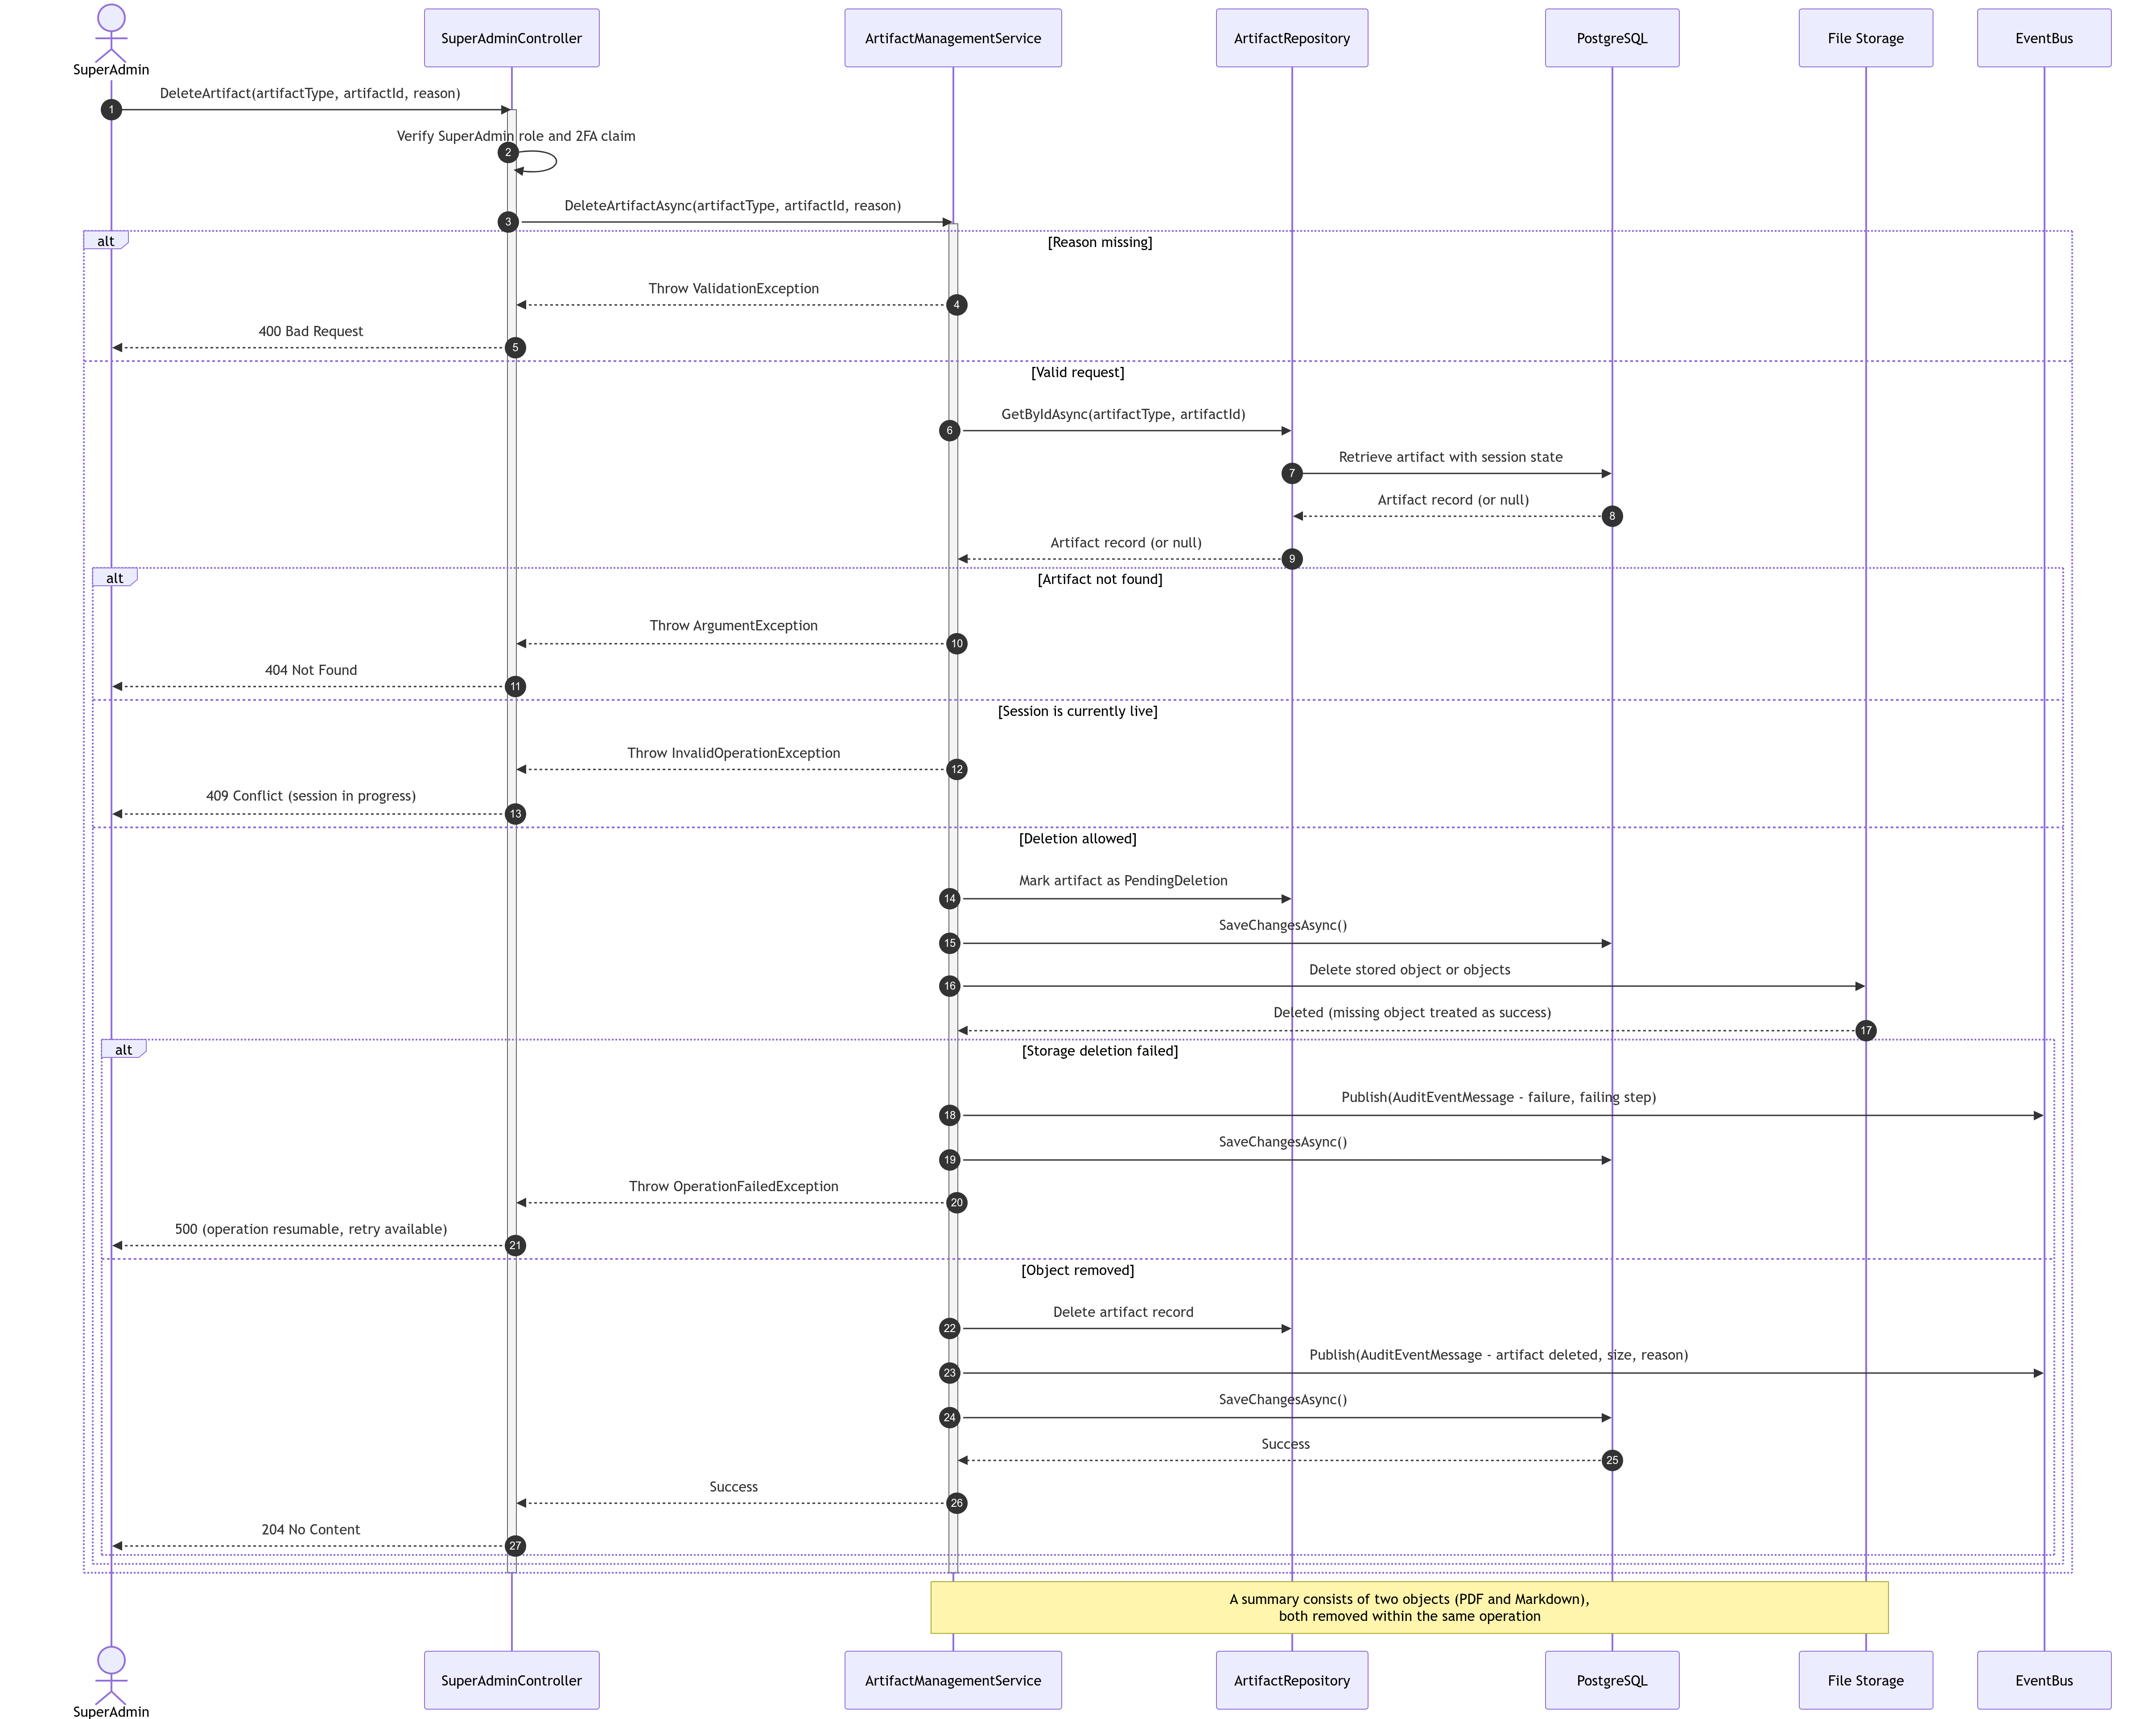
\includegraphics[width=\textwidth,height=0.8\textheight,keepaspectratio]{figures/image43.png}
  \caption{مخطط تسلسل النظام لحالة «حذف تسجيل أو ملخص»: يوضّح الرسائل المتبادلة بين الفاعل والنظام بوصفه صندوقًا أسود، أي دون إظهار الخدمات الداخلية التي تنفّذها.}
  \label{fig:image43}
\end{figure}

\subsubsection{مخطط تسلسل النظام لحالات استخدام الطالب}

\subsection{مخطط تسلسل النظام لحالات استخدام النظام}

\subsubsection{مخطط تسلسل النظام لحالة فهرسة ملفات الفصل}

\begin{figure}[htbp]
  \centering
  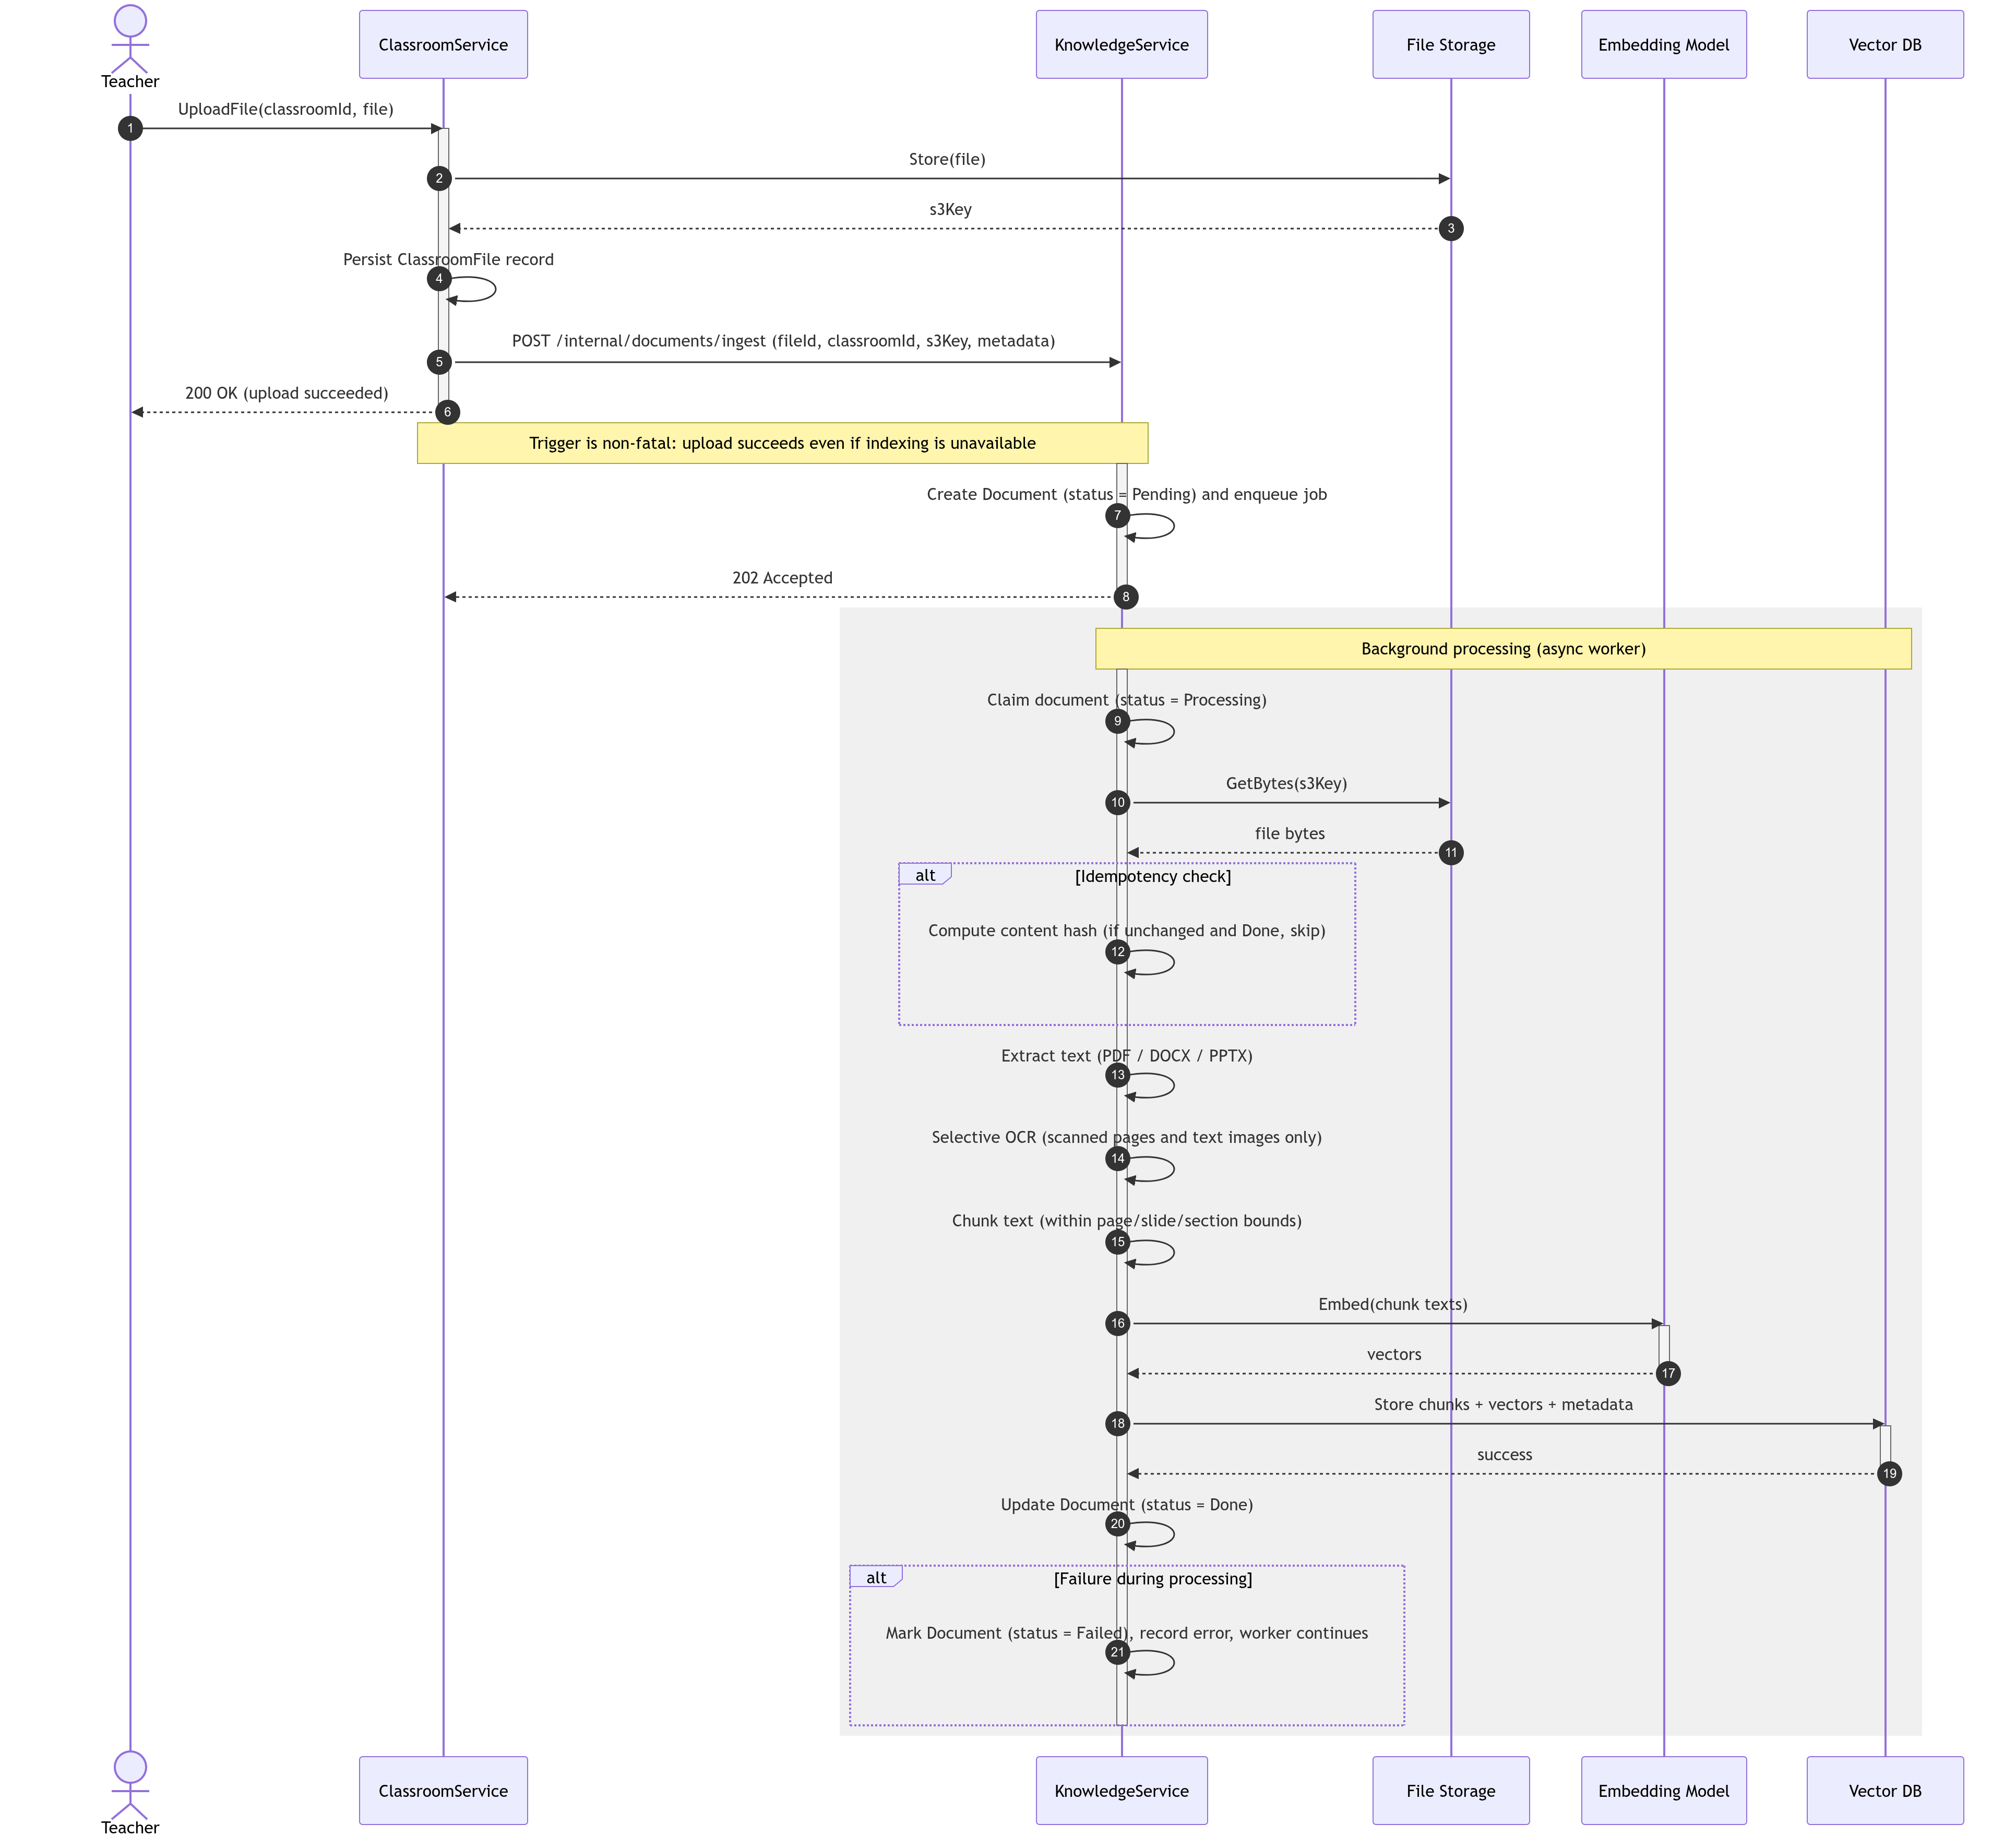
\includegraphics[width=\textwidth,height=0.8\textheight,keepaspectratio]{figures/image48.png}
  \caption{مخطط تسلسل النظام لحالة «فهرسة ملفات الفصل»: يوضّح الرسائل المتبادلة بين الفاعل والنظام بوصفه صندوقًا أسود، أي دون إظهار الخدمات الداخلية التي تنفّذها.}
  \label{fig:image48}
\end{figure}

\subsubsection{مخطط تسلسل النظام لحالة تحليل شرح المعلم مقابل المادة المرجعية}

\begin{figure}[htbp]
  \centering
  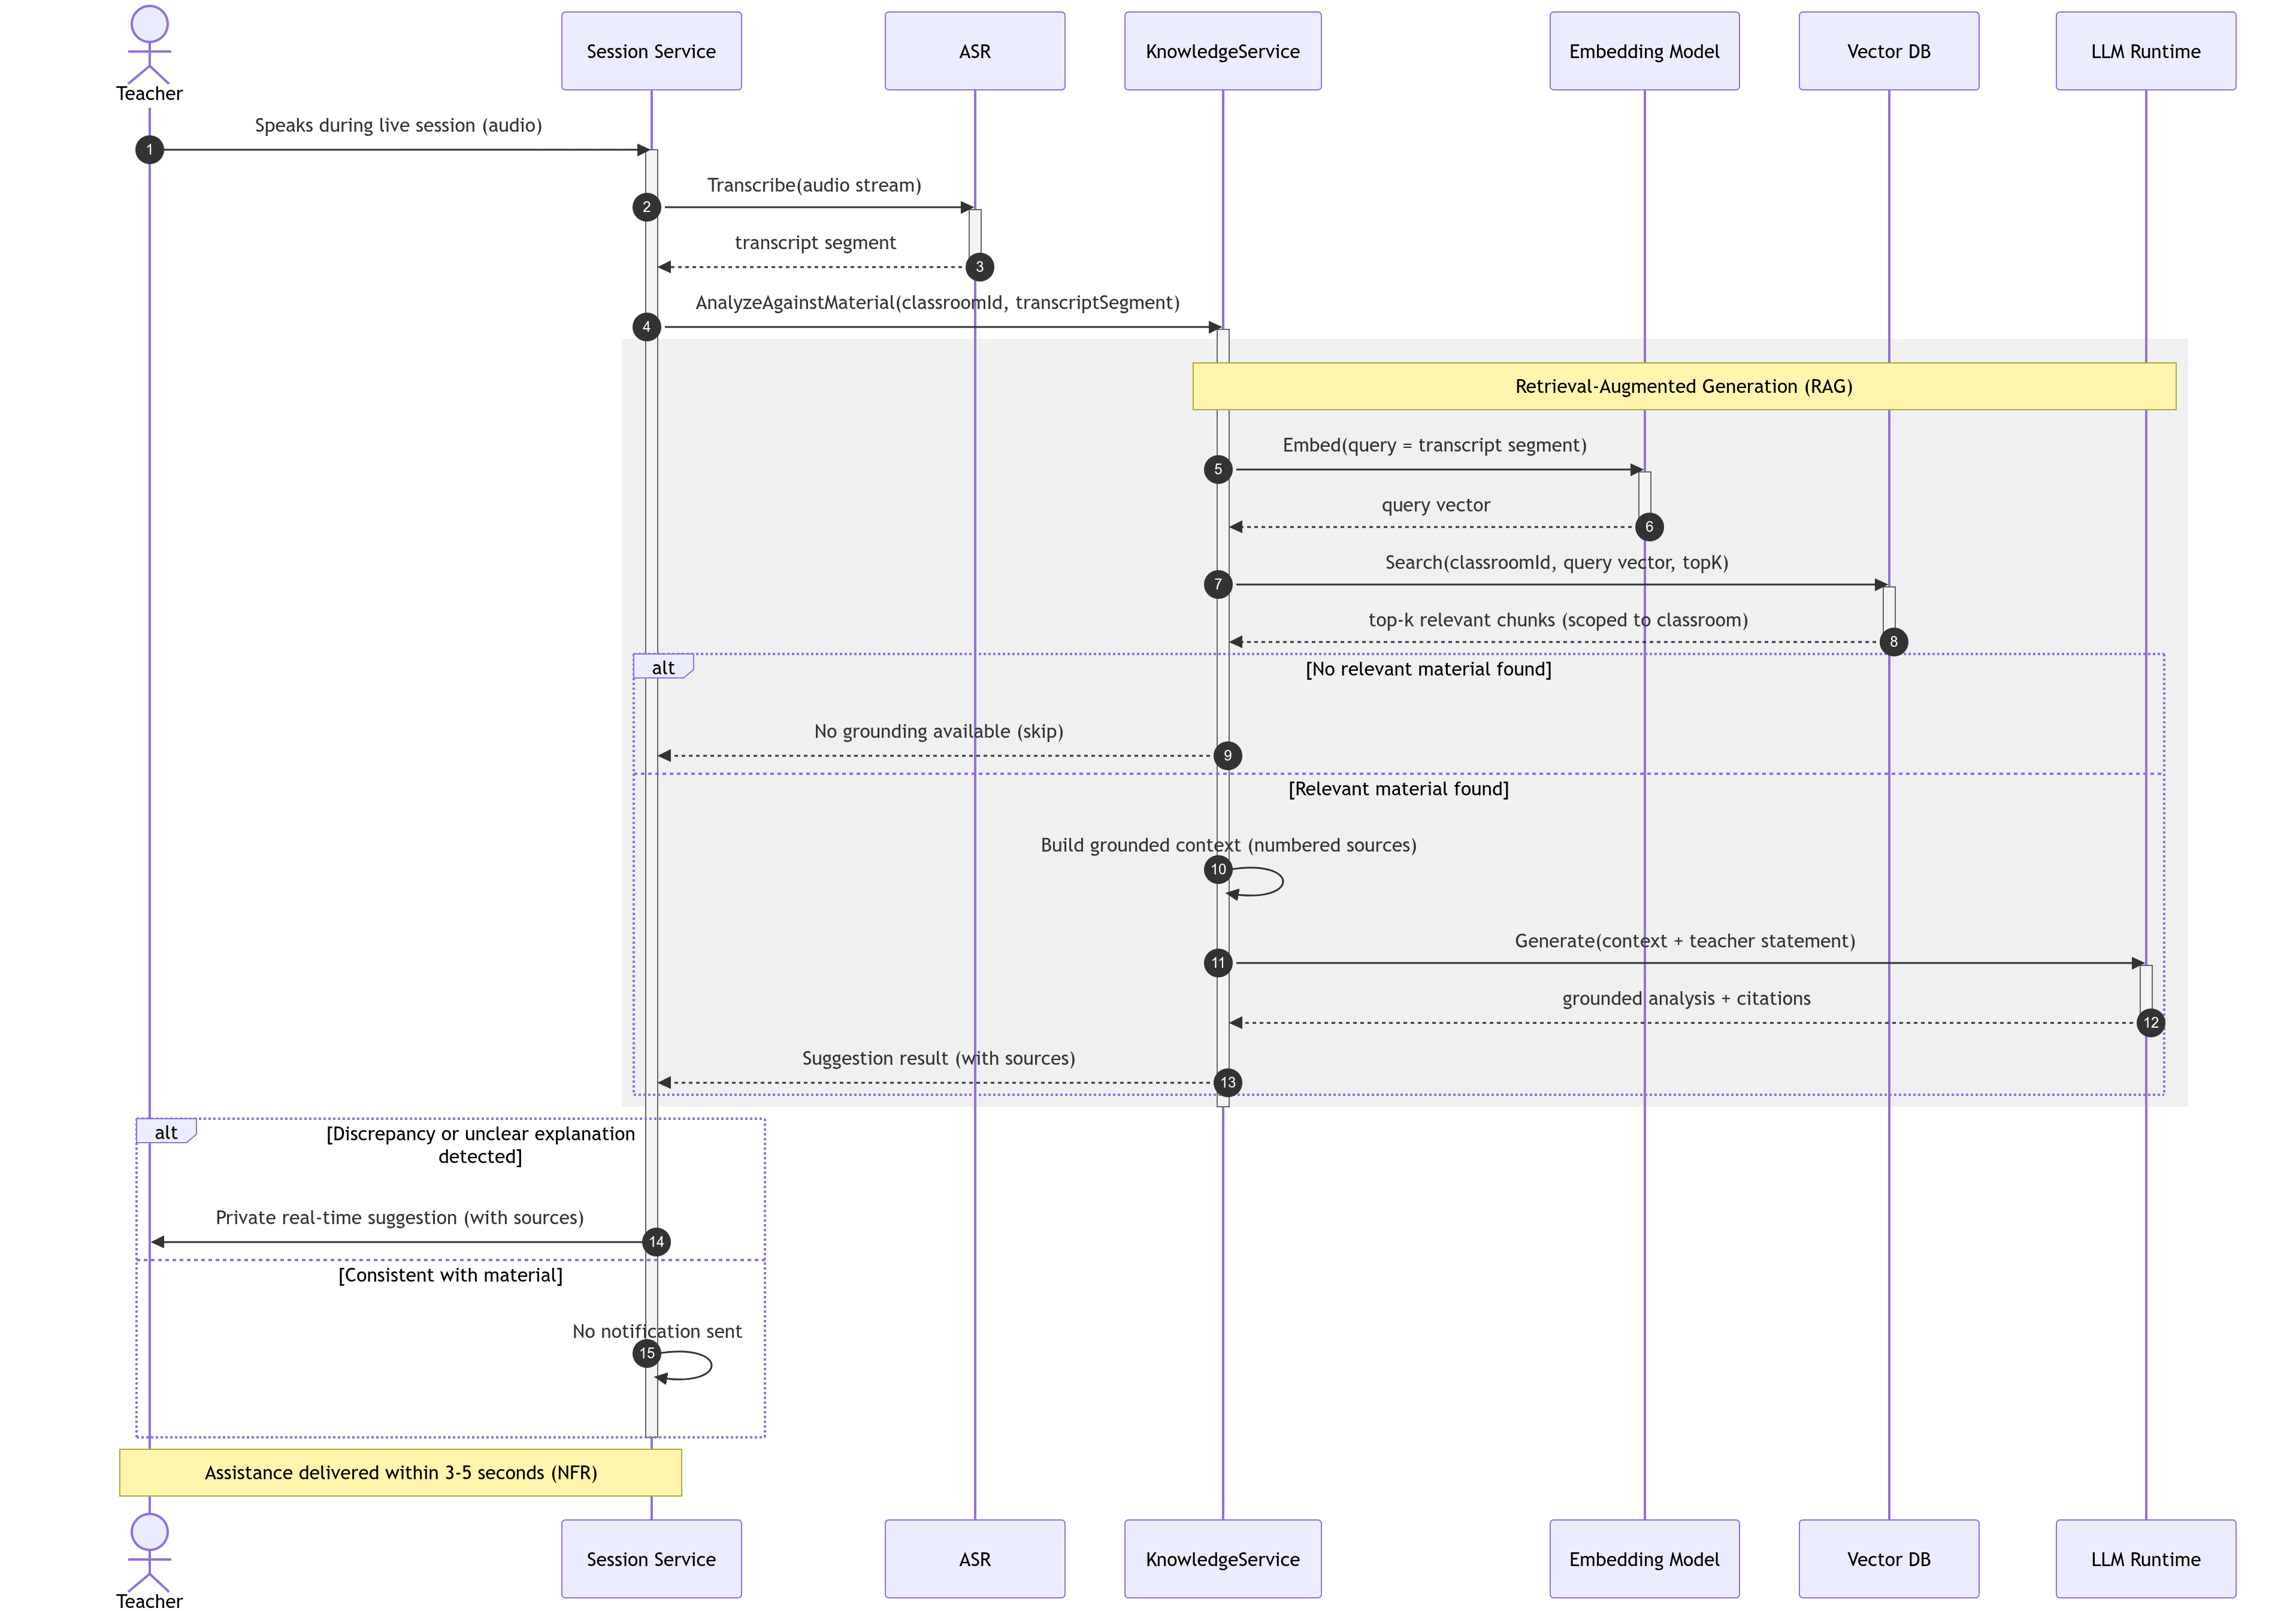
\includegraphics[width=\textwidth,height=0.8\textheight,keepaspectratio]{figures/image49.png}
  \caption{مخطط تسلسل النظام لحالة «تحليل شرح المعلم مقابل المادة المرجعية»: يوضّح الرسائل المتبادلة بين الفاعل والنظام بوصفه صندوقًا أسود، أي دون إظهار الخدمات الداخلية التي تنفّذها.}
  \label{fig:image49}
\end{figure}

\subsubsection{تدفّق الحلقة الحيّة}
\label{subsubsec:flow-live-loop}

يعرض الشكل~\ref{fig:arch-03} الحلقة التي تعمل طوال الجلسة: التقاط الصوت، وتحويله إلى نص، وكشف اكتمال الفكرة، وتقييمها مقابل المصادر المفهرسة، ثمّ اتّخاذ قرار التدخّل من عدمه.

\begin{figure}[htbp]
  \centering
  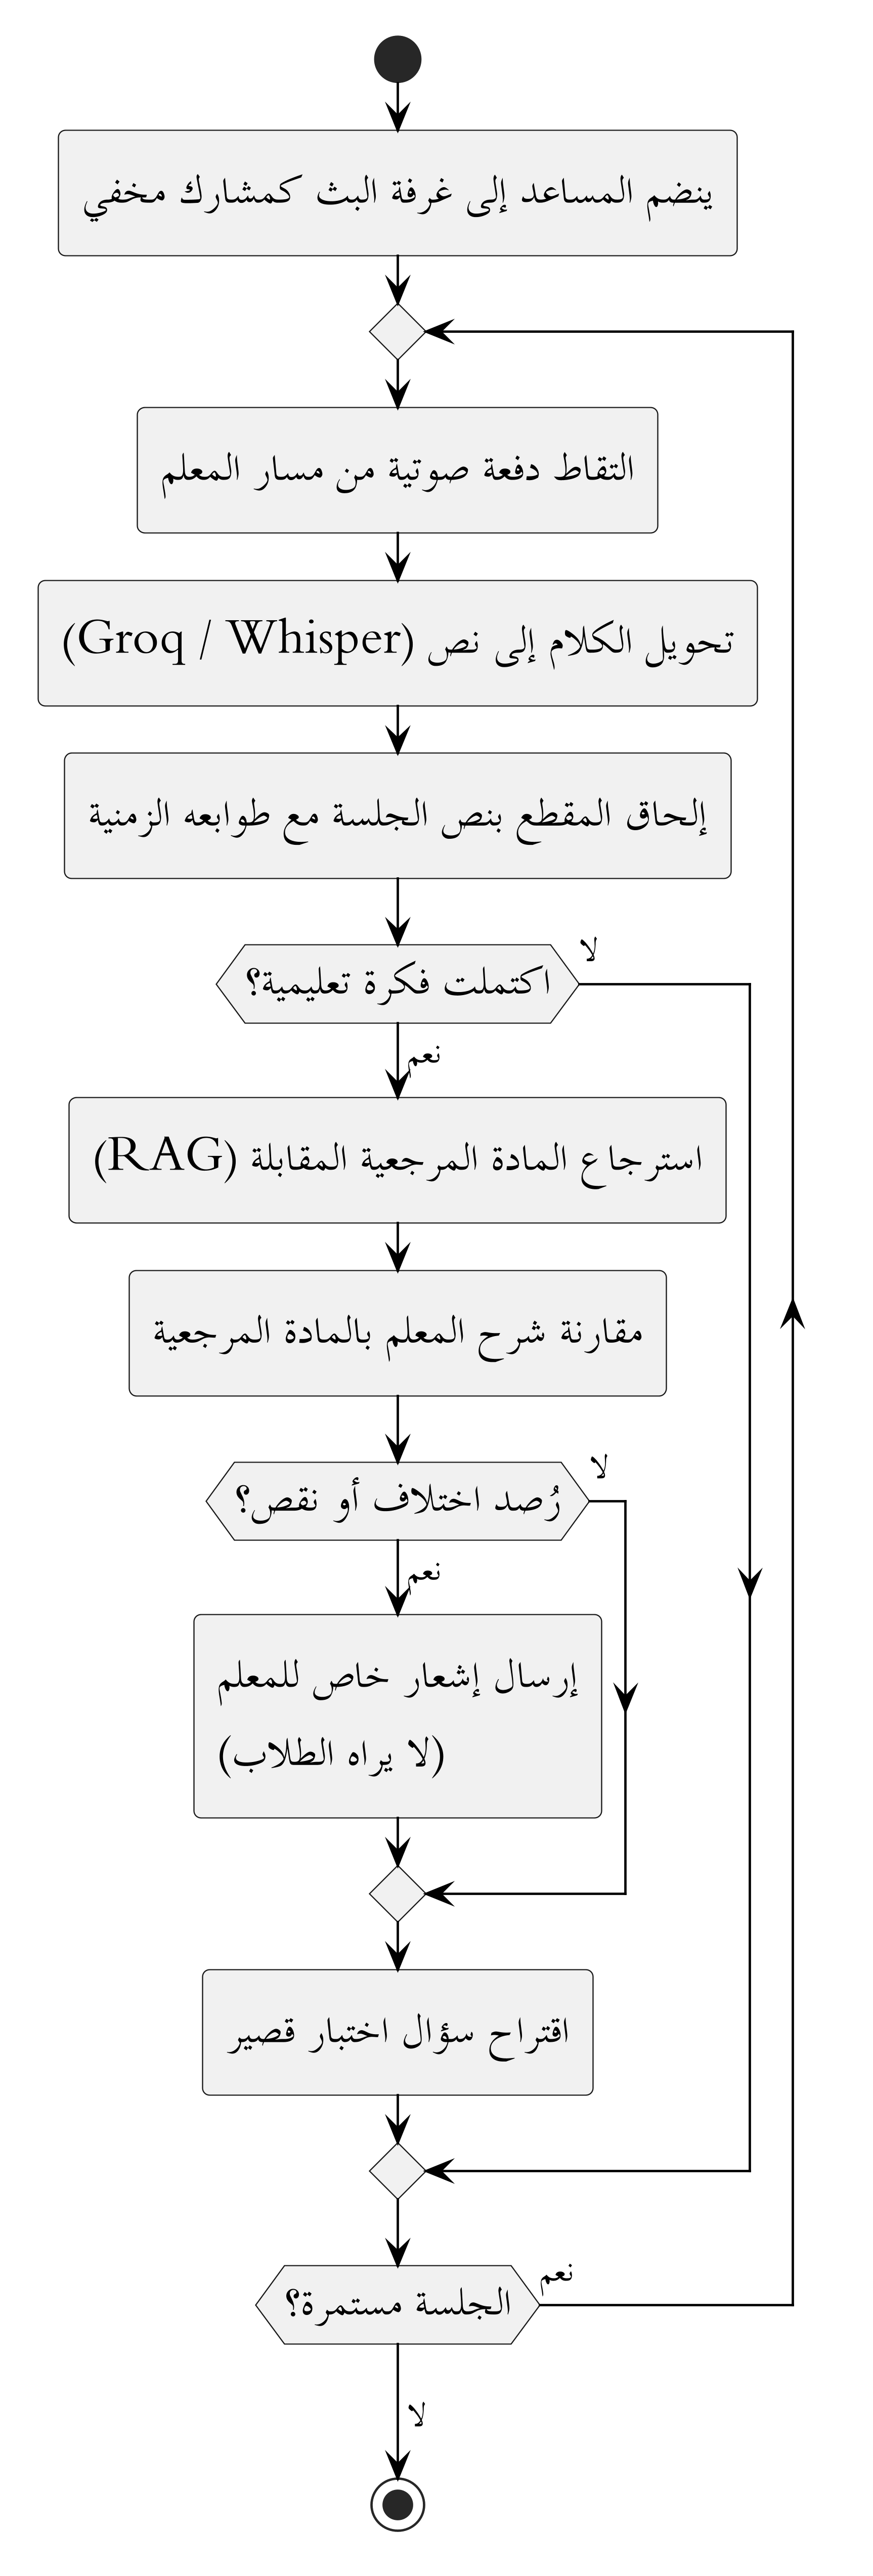
\includegraphics[width=\textwidth,height=0.8\textheight,keepaspectratio]{figures/arch-03-live-assistant.png}
  \caption{تدفّق الحلقة الحيّة في خدمة المساعد المباشر.}
  \label{fig:arch-03}
\end{figure}

\subsubsection{تدفّق تسجيل الجلسة وحفظها}
\label{subsubsec:flow-recording}

يبيّن الشكل~\ref{fig:flow-03} تدفّق تسجيل الجلسة وما اعتُمد فيه من حجزٍ ومُصالِحٍ دوريّ لمعالجة التبعية لنظام خارجي.

\begin{figure}[htbp]
  \centering
  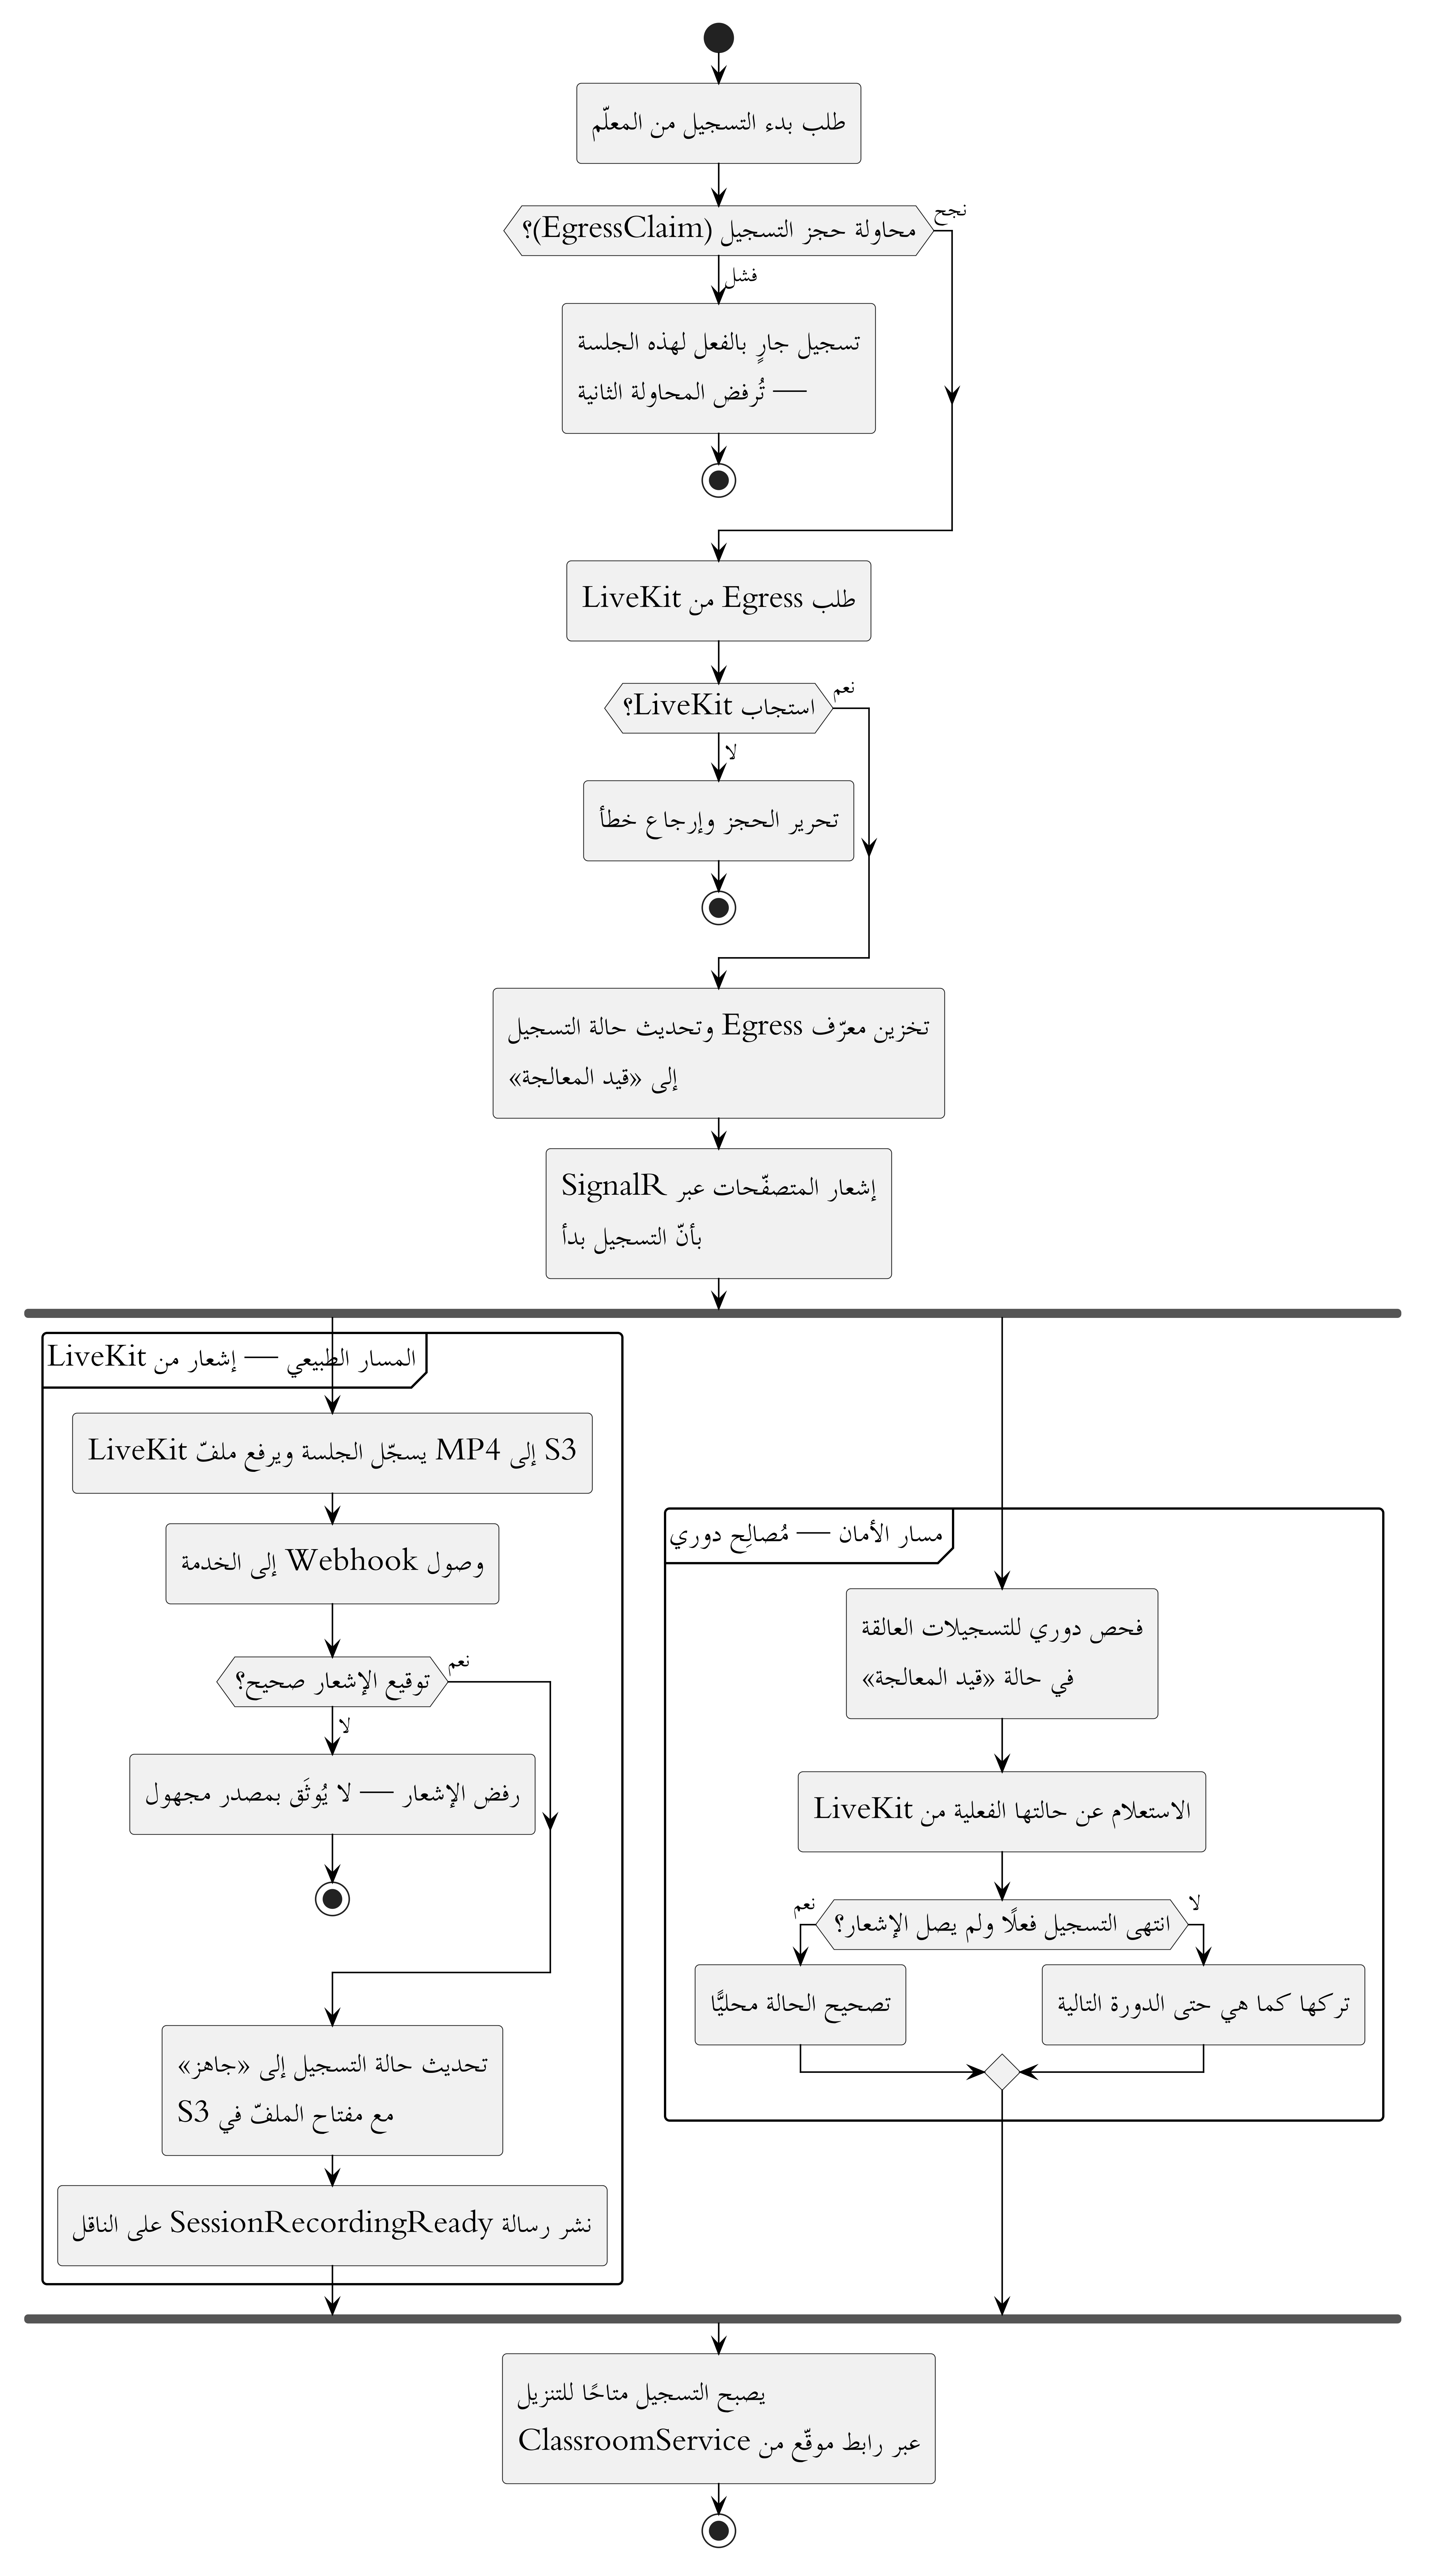
\includegraphics[width=\textwidth,height=0.8\textheight,keepaspectratio]{figures/flow-03-recording-egress.png}
  \caption{تدفّق تسجيل الجلسة وحفظها في مخزن الملفّات.}
  \label{fig:flow-03}
\end{figure}

\noindent يعتمد تدفّق التسجيل على نظام خارجي، ولا تستطيع خدمة البث إتمامه وحدها. وقد بُيّنت معالجة هذه التبعية في الشكل~\ref{fig:flow-03}.

واعتُمدت آليتان متكاملتان لمعالجة هذه التبعية:

\begin{enumerate}
  \item \textbf{الحجز} (\en{EgressClaim}): يمنع بدء تسجيلين متوازيين للجلسة نفسها، وهو احتمال قائم عند الضغط على زرّ التسجيل مرّتين قبل وصول جواب \en{LiveKit} عن الطلب الأول.
  \item \textbf{المُصالِح الدوري} (\en{Reconciler}): يفحص دوريًّا التسجيلات العالقة في حالة المعالجة، ويستعلم عن حالتها الفعلية من \en{LiveKit}، ويصحّحها محلّيًّا. ويحافظ ذلك على صحّة الحالة حتى عند فقد الإشعار.
\end{enumerate}

\subsubsection{تدفّق إرسال الإشعارات البريدية}
\label{subsubsec:flow-email}

\begin{figure}[htbp]
  \centering
  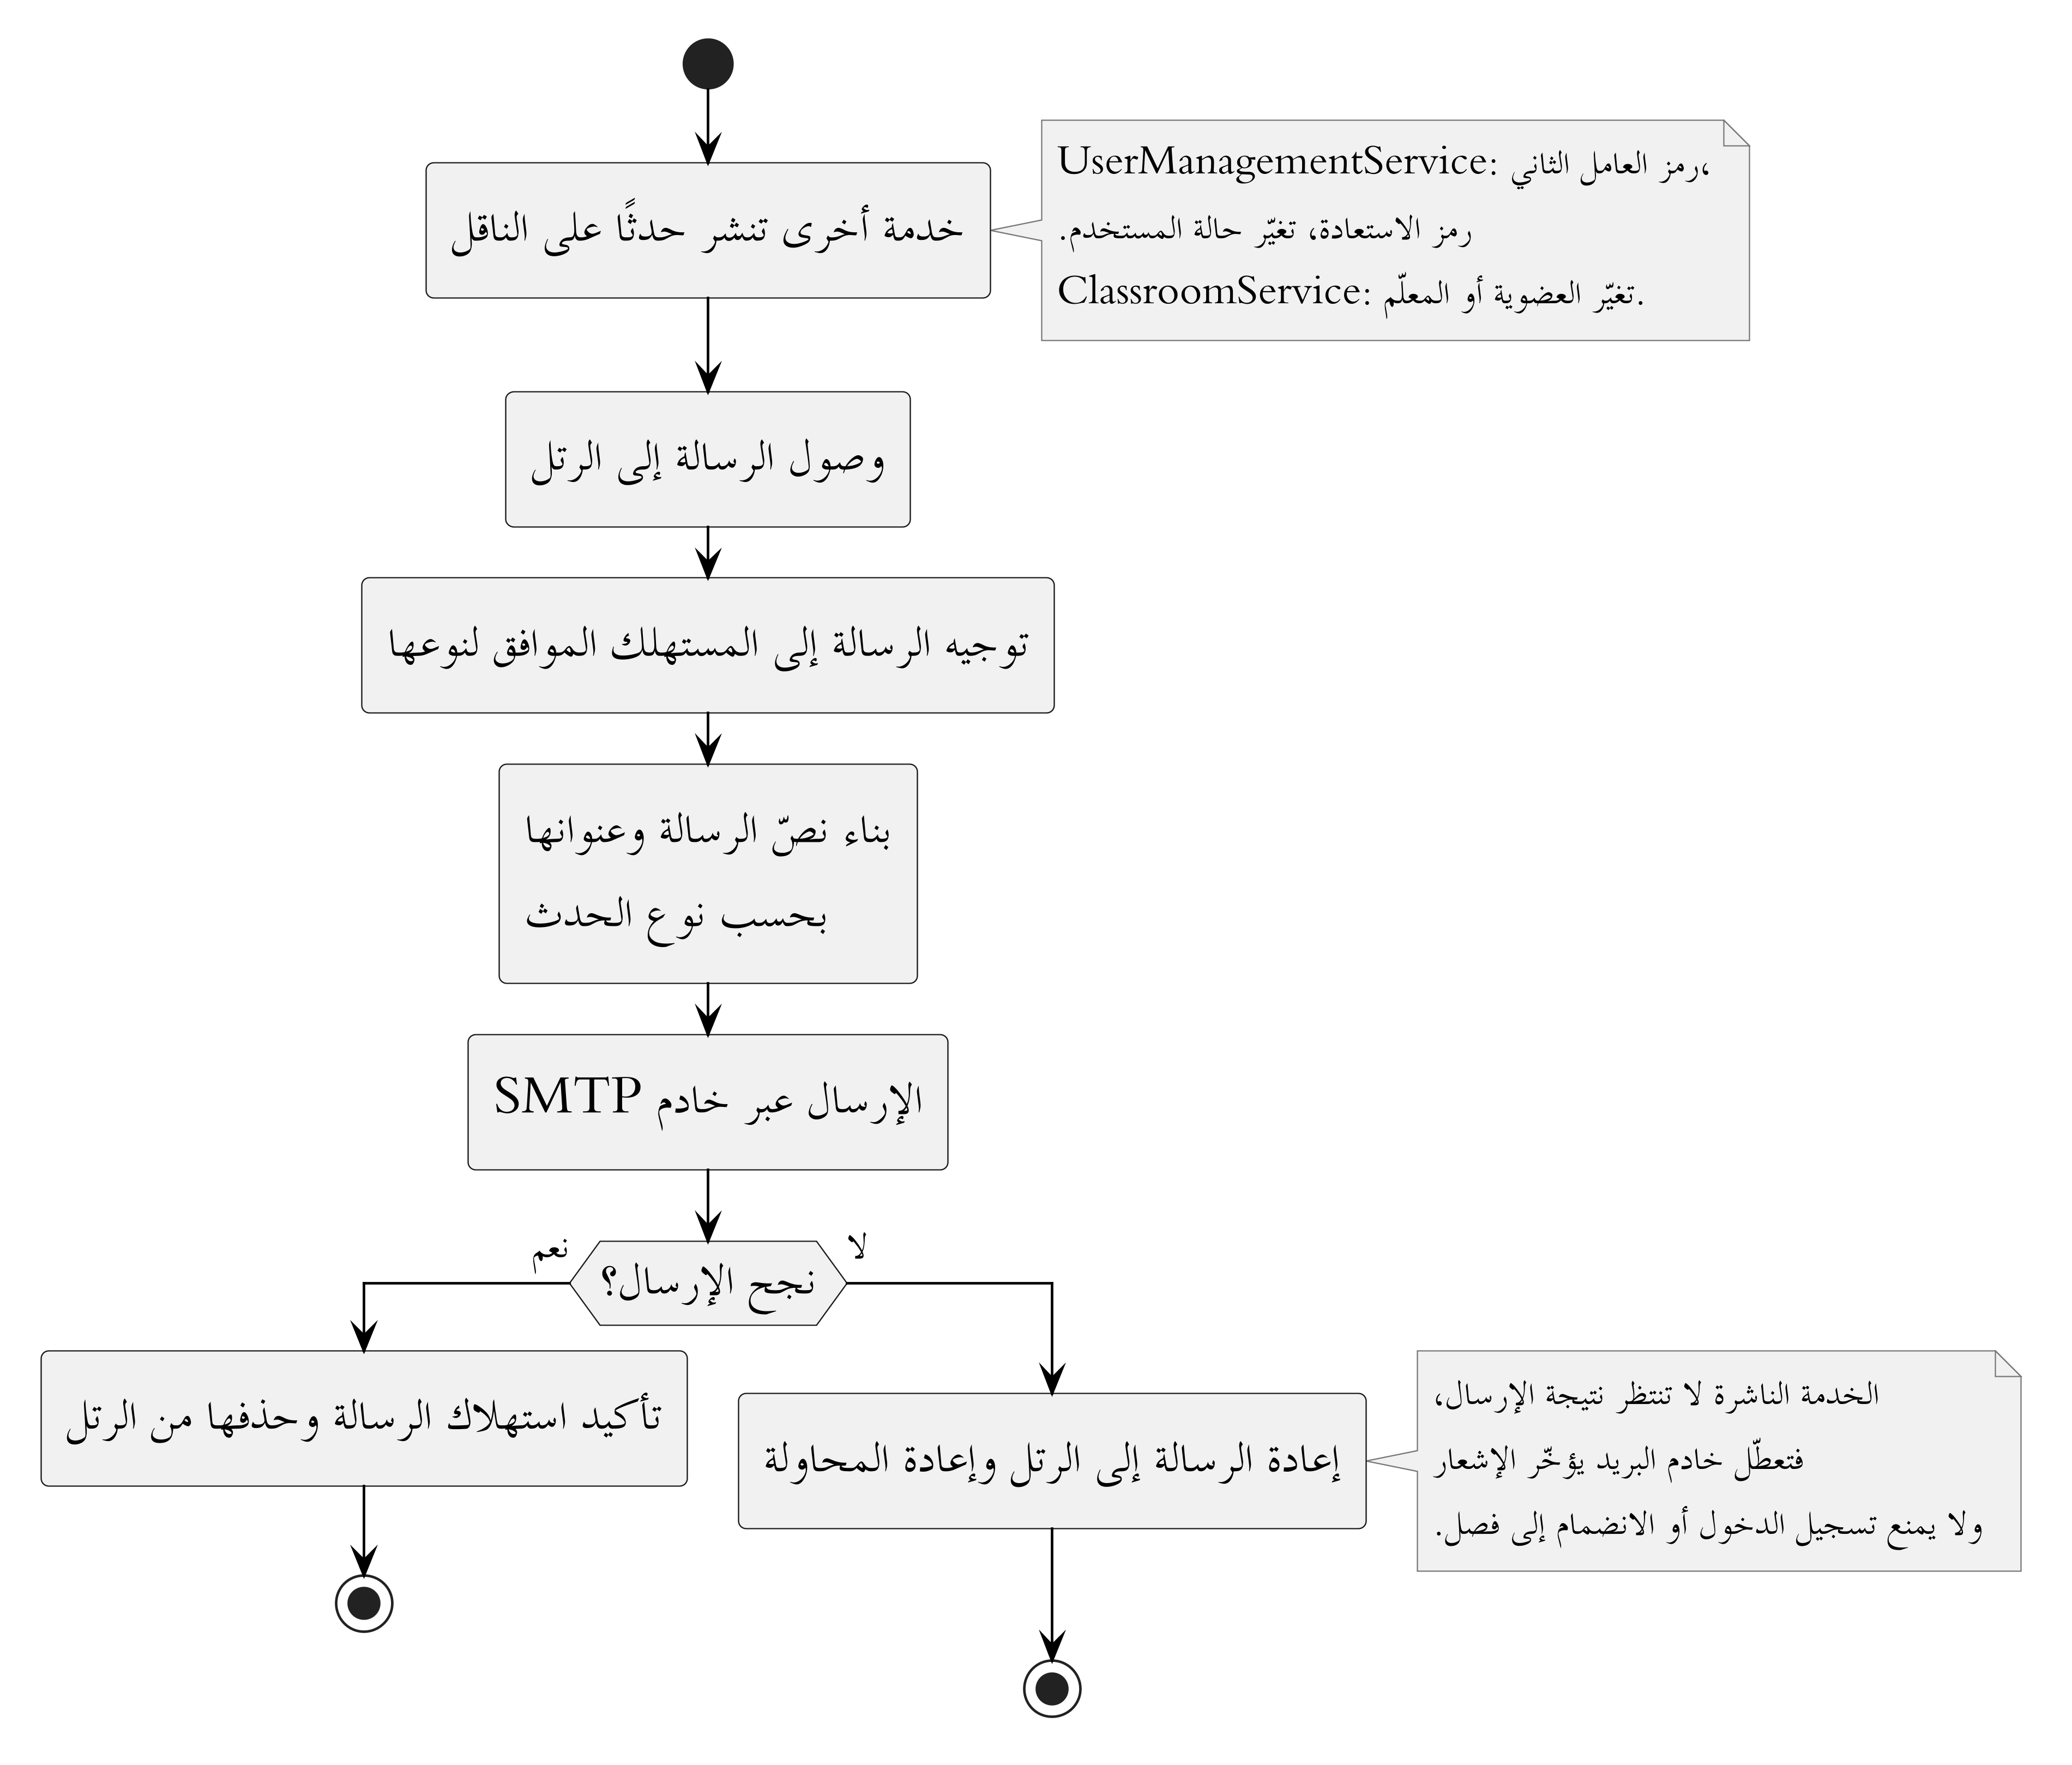
\includegraphics[width=\textwidth,height=0.8\textheight,keepaspectratio]{figures/flow-04-email-dispatch.png}
  \caption{تدفّق إرسال الإشعارات البريدية.}
  \label{fig:flow-04}
\end{figure}

\noindent وقد بُيّن مسار الإشعار من لحظة نشره إلى لحظة تسليمه في الشكل~\ref{fig:flow-04}.

ويحقّق عزل هذه المسؤولية في خدمة مستهلِكة فكَّ الارتباط الزمني، إذ لا تنتظر الخدمة الناشرة نتيجة الإرسال. ويؤدّي تعطّل خادم البريد عندئذٍ إلى تأخير وصول الإشعارات دون تعطيل تسجيل الدخول أو التسجيل أو الانضمام إلى فصل.

\subsubsection{تدفّق استيعاب المستندات وفهرستها}
\label{subsubsec:flow-ingestion}

يبيّن الشكل~\ref{fig:arch-02} مراحل خط أنابيب الاستيعاب، وتُعالَج جميعها بشكل غير متزامن في الخلفية تفادياً لتعطيل رفع الملفّ بانتظار المعالجة الثقيلة.

\begin{figure}[htbp]
  \centering
  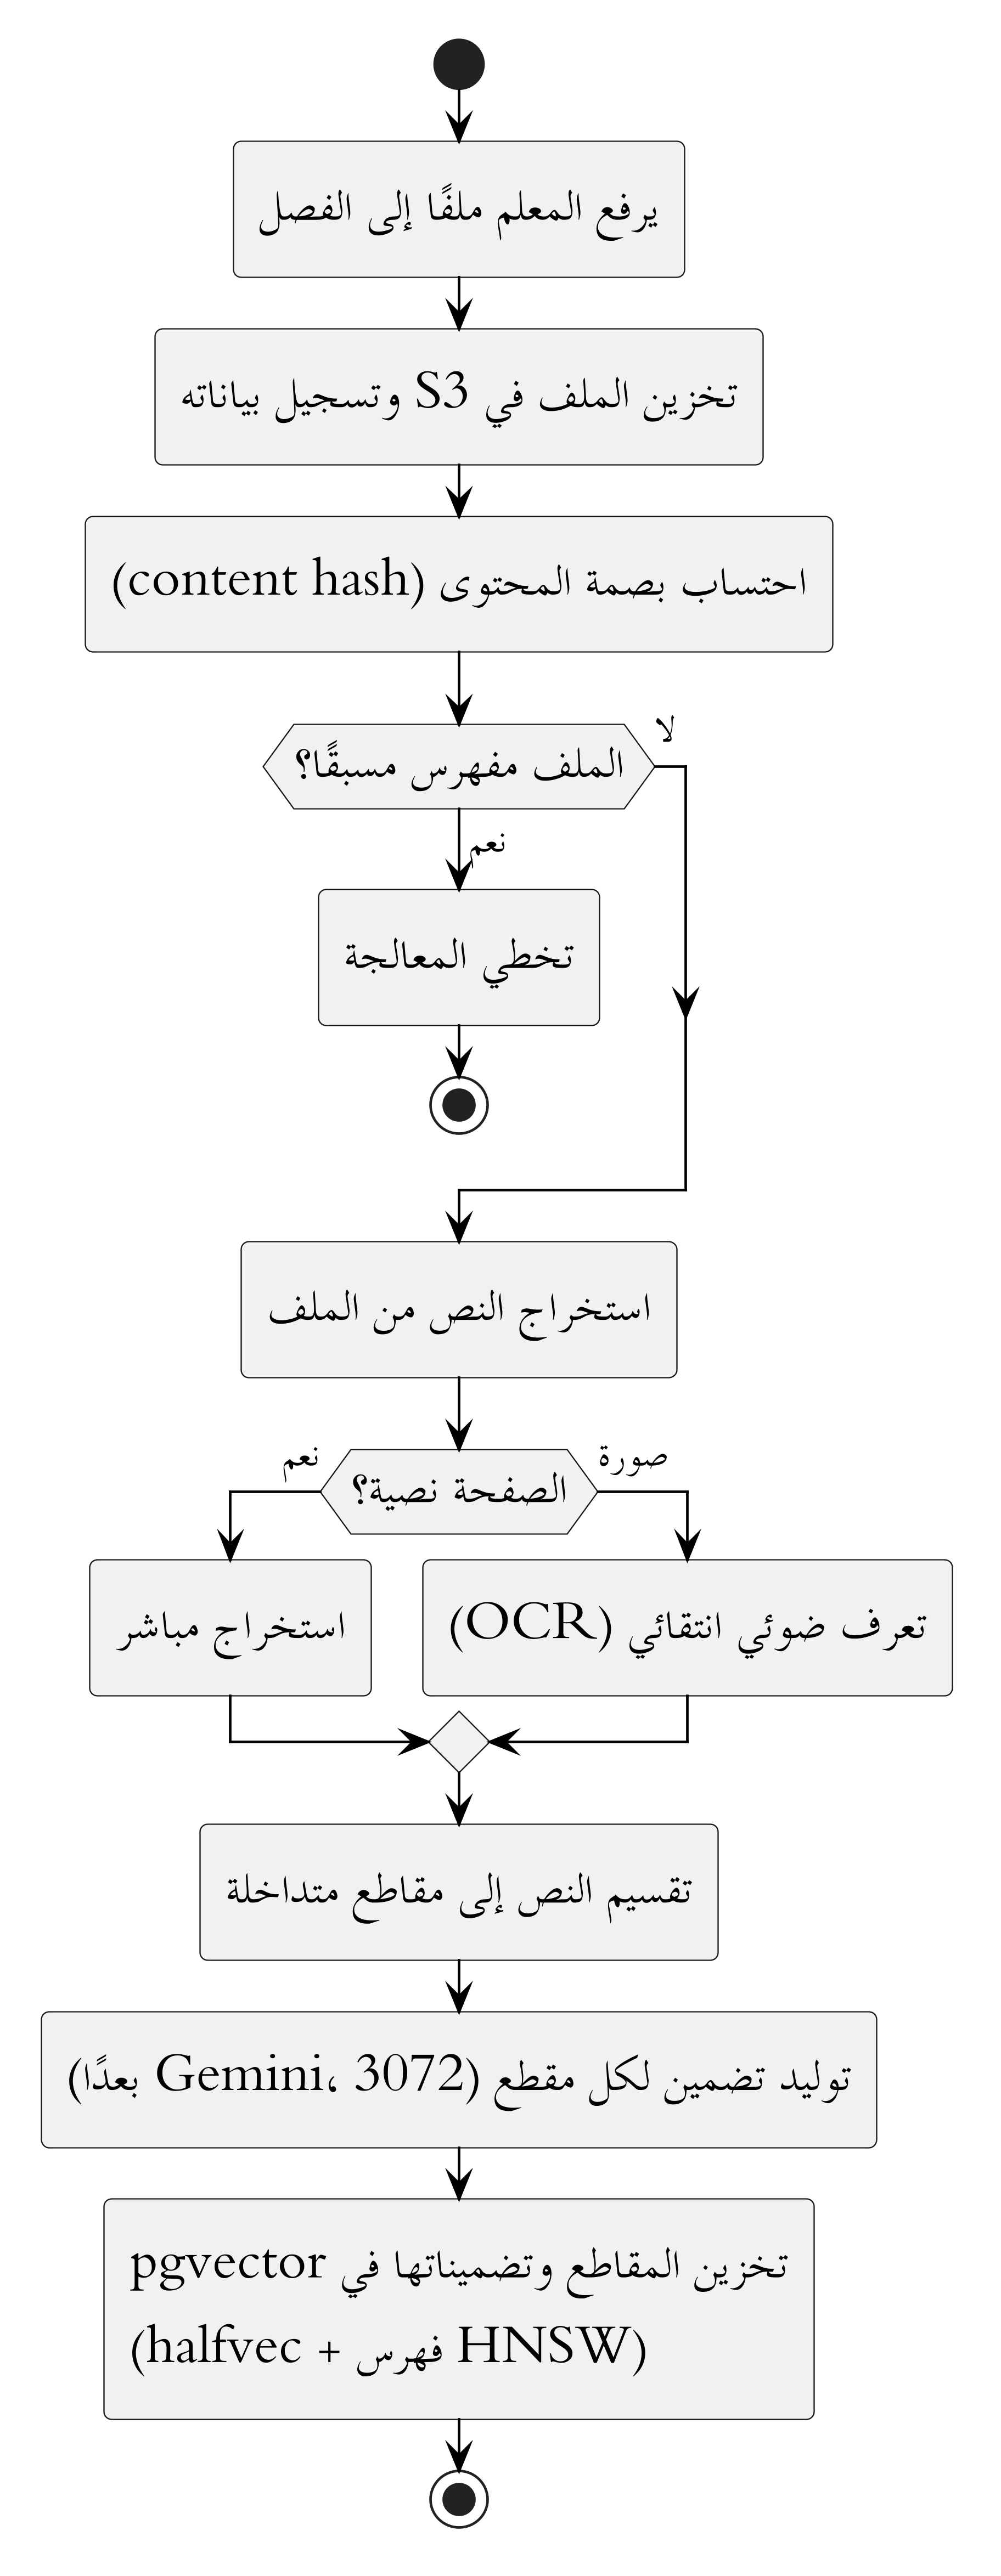
\includegraphics[width=\textwidth,height=0.8\textheight,keepaspectratio]{figures/arch-02-rag-pipeline.png}
  \caption{تدفّق استيعاب المستندات وفهرستها في خدمة الاسترجاع.}
  \label{fig:arch-02}
\end{figure}

% CH2-REF: originally ended "والكلفة (القسم~\ref{subsec:text-extraction-ocr})." — restore with chapter 2.
\noindent واعتُمد عامل معالجة محدود التزامن، ممّا يتيح التحكّم في استهلاك الموارد ويمنع استنزاف الجهاز عند معالجة عدّة ملفّات معاً. وصُمّمت المعالجة خاملة التكرار (\en{Idempotent})، فلا تُعاد فهرسة الملفّ نفسه دون تغيّر في محتواه، مع دعم إعادة الفهرسة عند تغيّره. ويُطبَّق التعرّف الضوئي (\en{OCR}) على الصفحات الممسوحة والصور الحاملة للنص فقط، موازنةً بين الدقة والكلفة.

ويقوم خط الأنابيب على نمط المنافذ والمحوِّلات، فيُحصر استبدال مزوّد التضمين أو محرّك التعرّف الضوئي في محوِّل واحد دون تعديل منطق الخط. ويعرض الشكل~\ref{fig:class-01} هذا التصميم.

\begin{figure}[htbp]
  \centering
  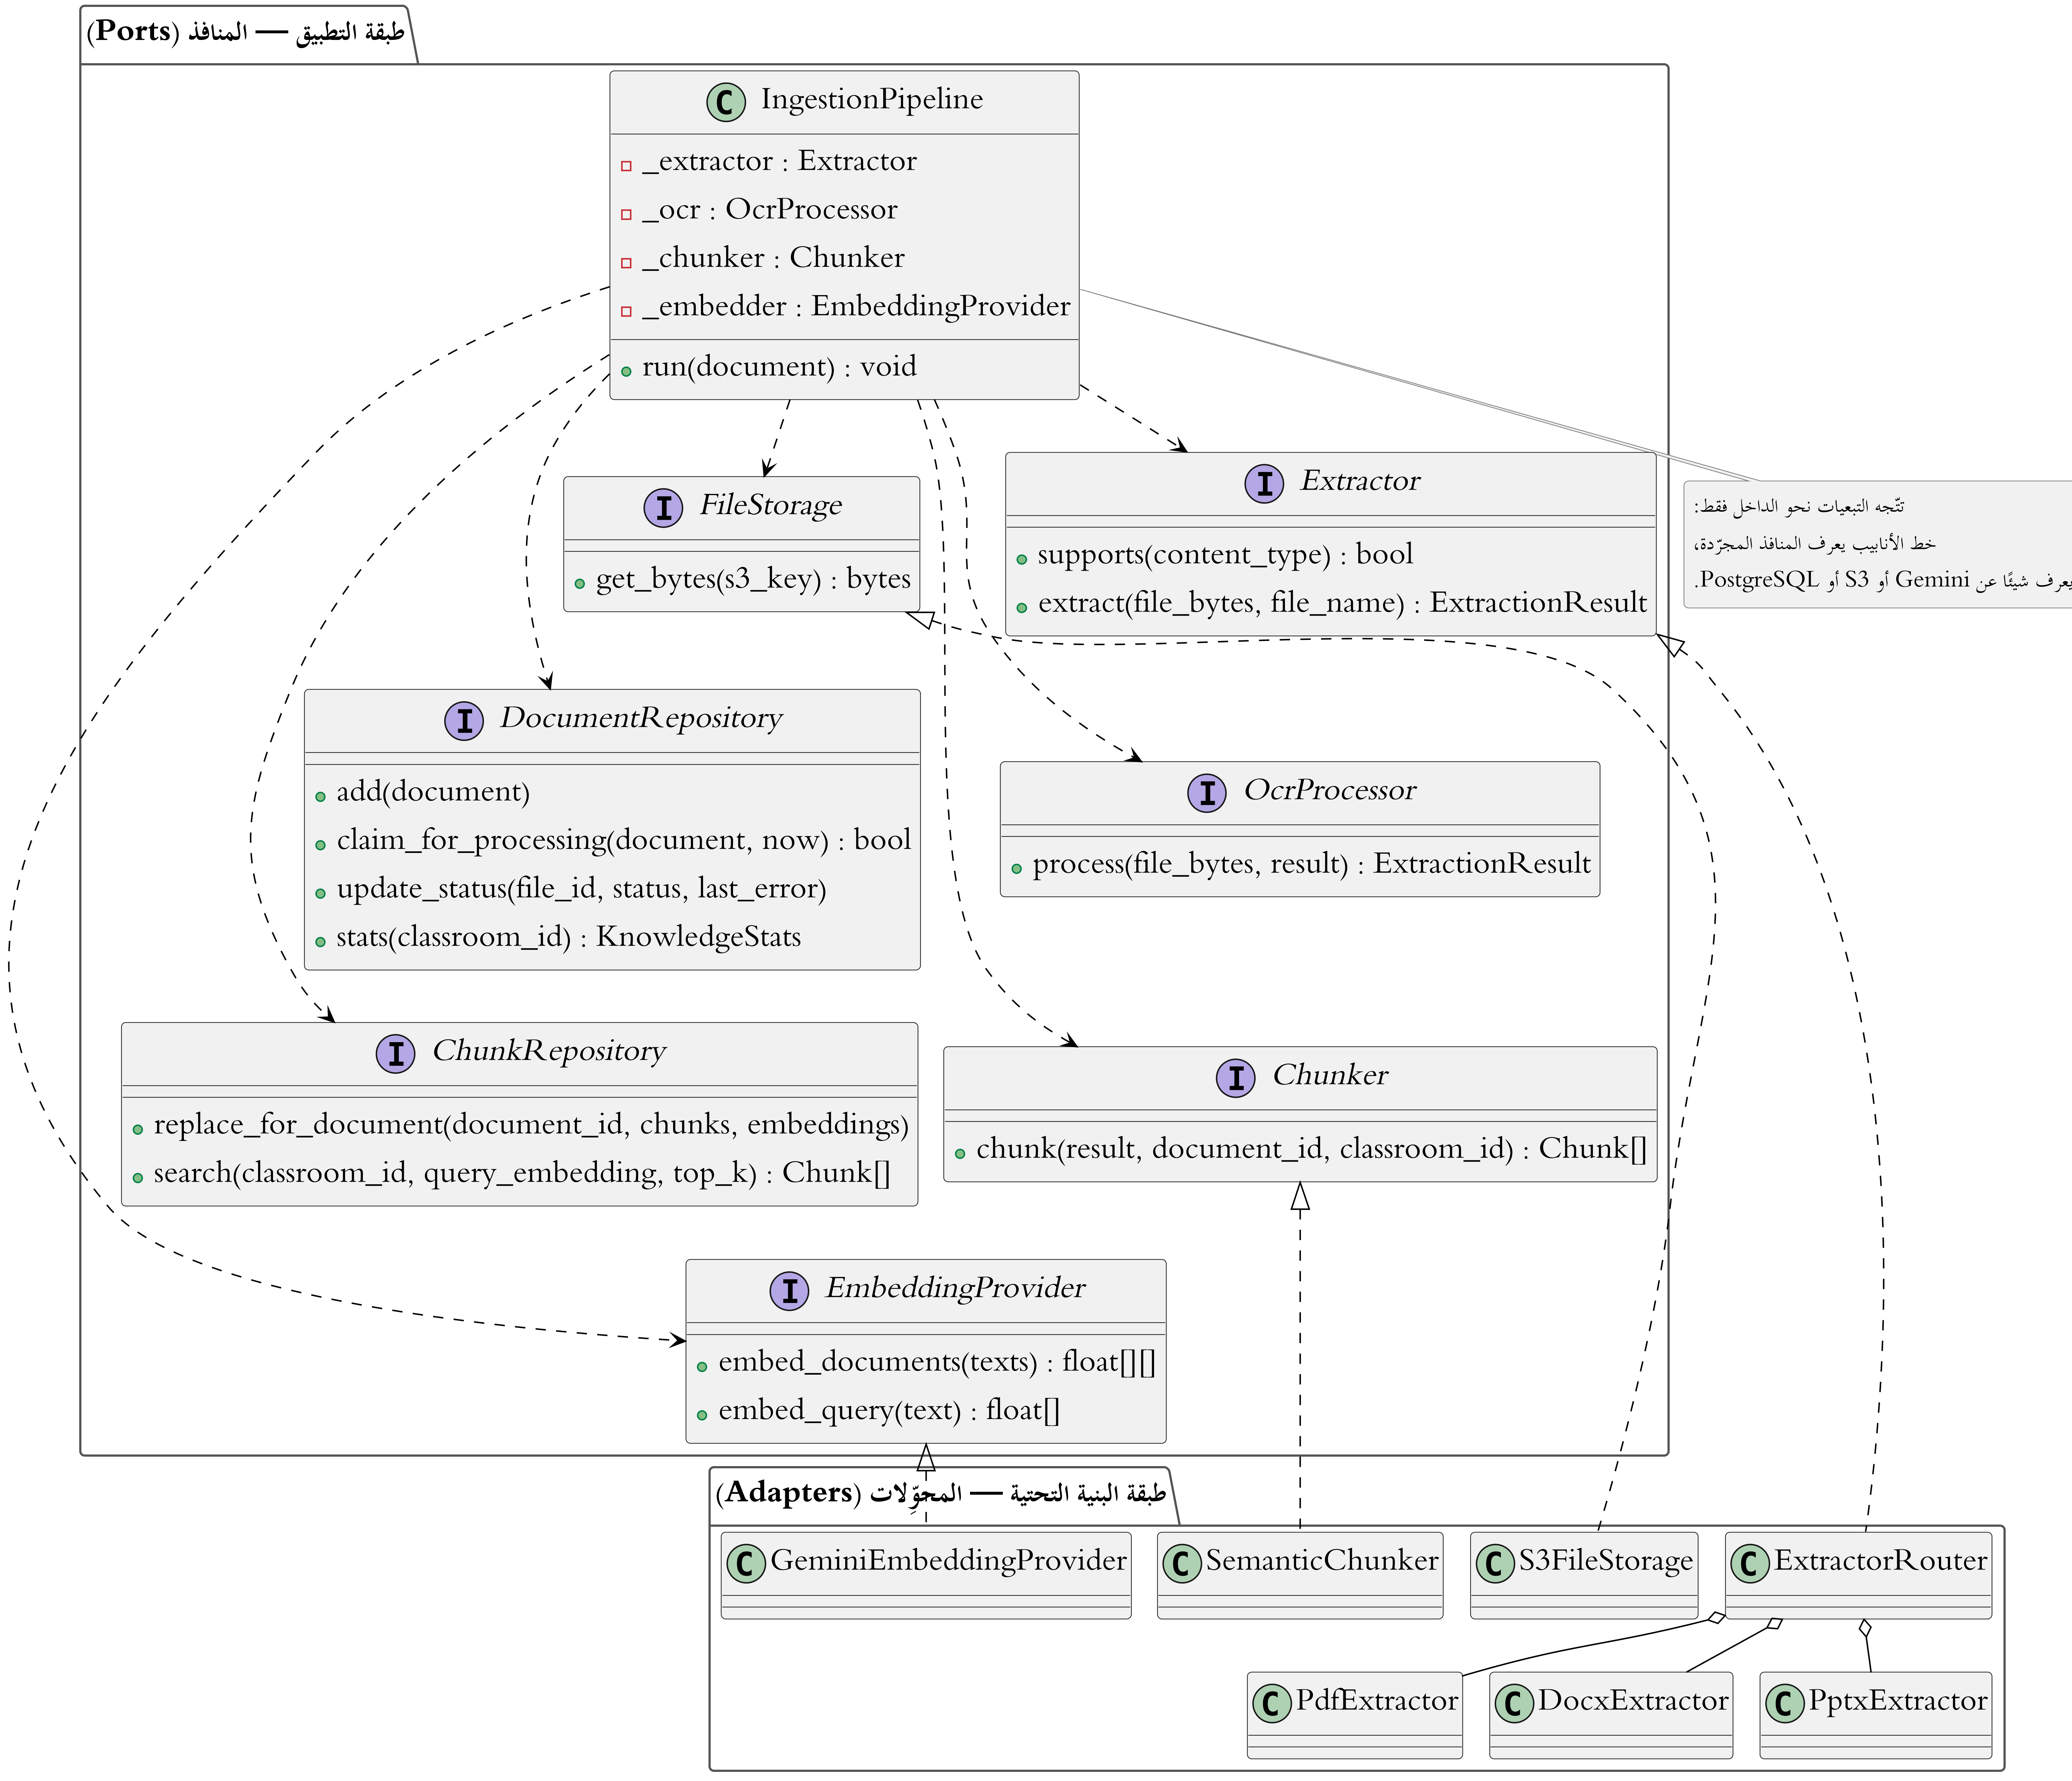
\includegraphics[width=\textwidth,height=0.8\textheight,keepaspectratio]{figures/class-01-ports-adapters.png}
  \caption{مخطط الصفوف لنمط المنافذ والمحوِّلات في خط أنابيب الاستيعاب.}
  \label{fig:class-01}
\end{figure}

\subsubsection{تدفّق الاسترجاع والإجابة}
\label{subsubsec:flow-retrieval}

يبيّن الشكل~\ref{fig:arch-02b} مسار الإجابة عن سؤال: تضمين السؤال، ثمّ البحث الدلالي المقصور على الفصل، ثمّ بناء السياق ضمن حدّ الرموز المتاح، ثمّ توليد الإجابة مؤصَّلةً في المقاطع المسترجَعة.

\begin{figure}[htbp]
  \centering
  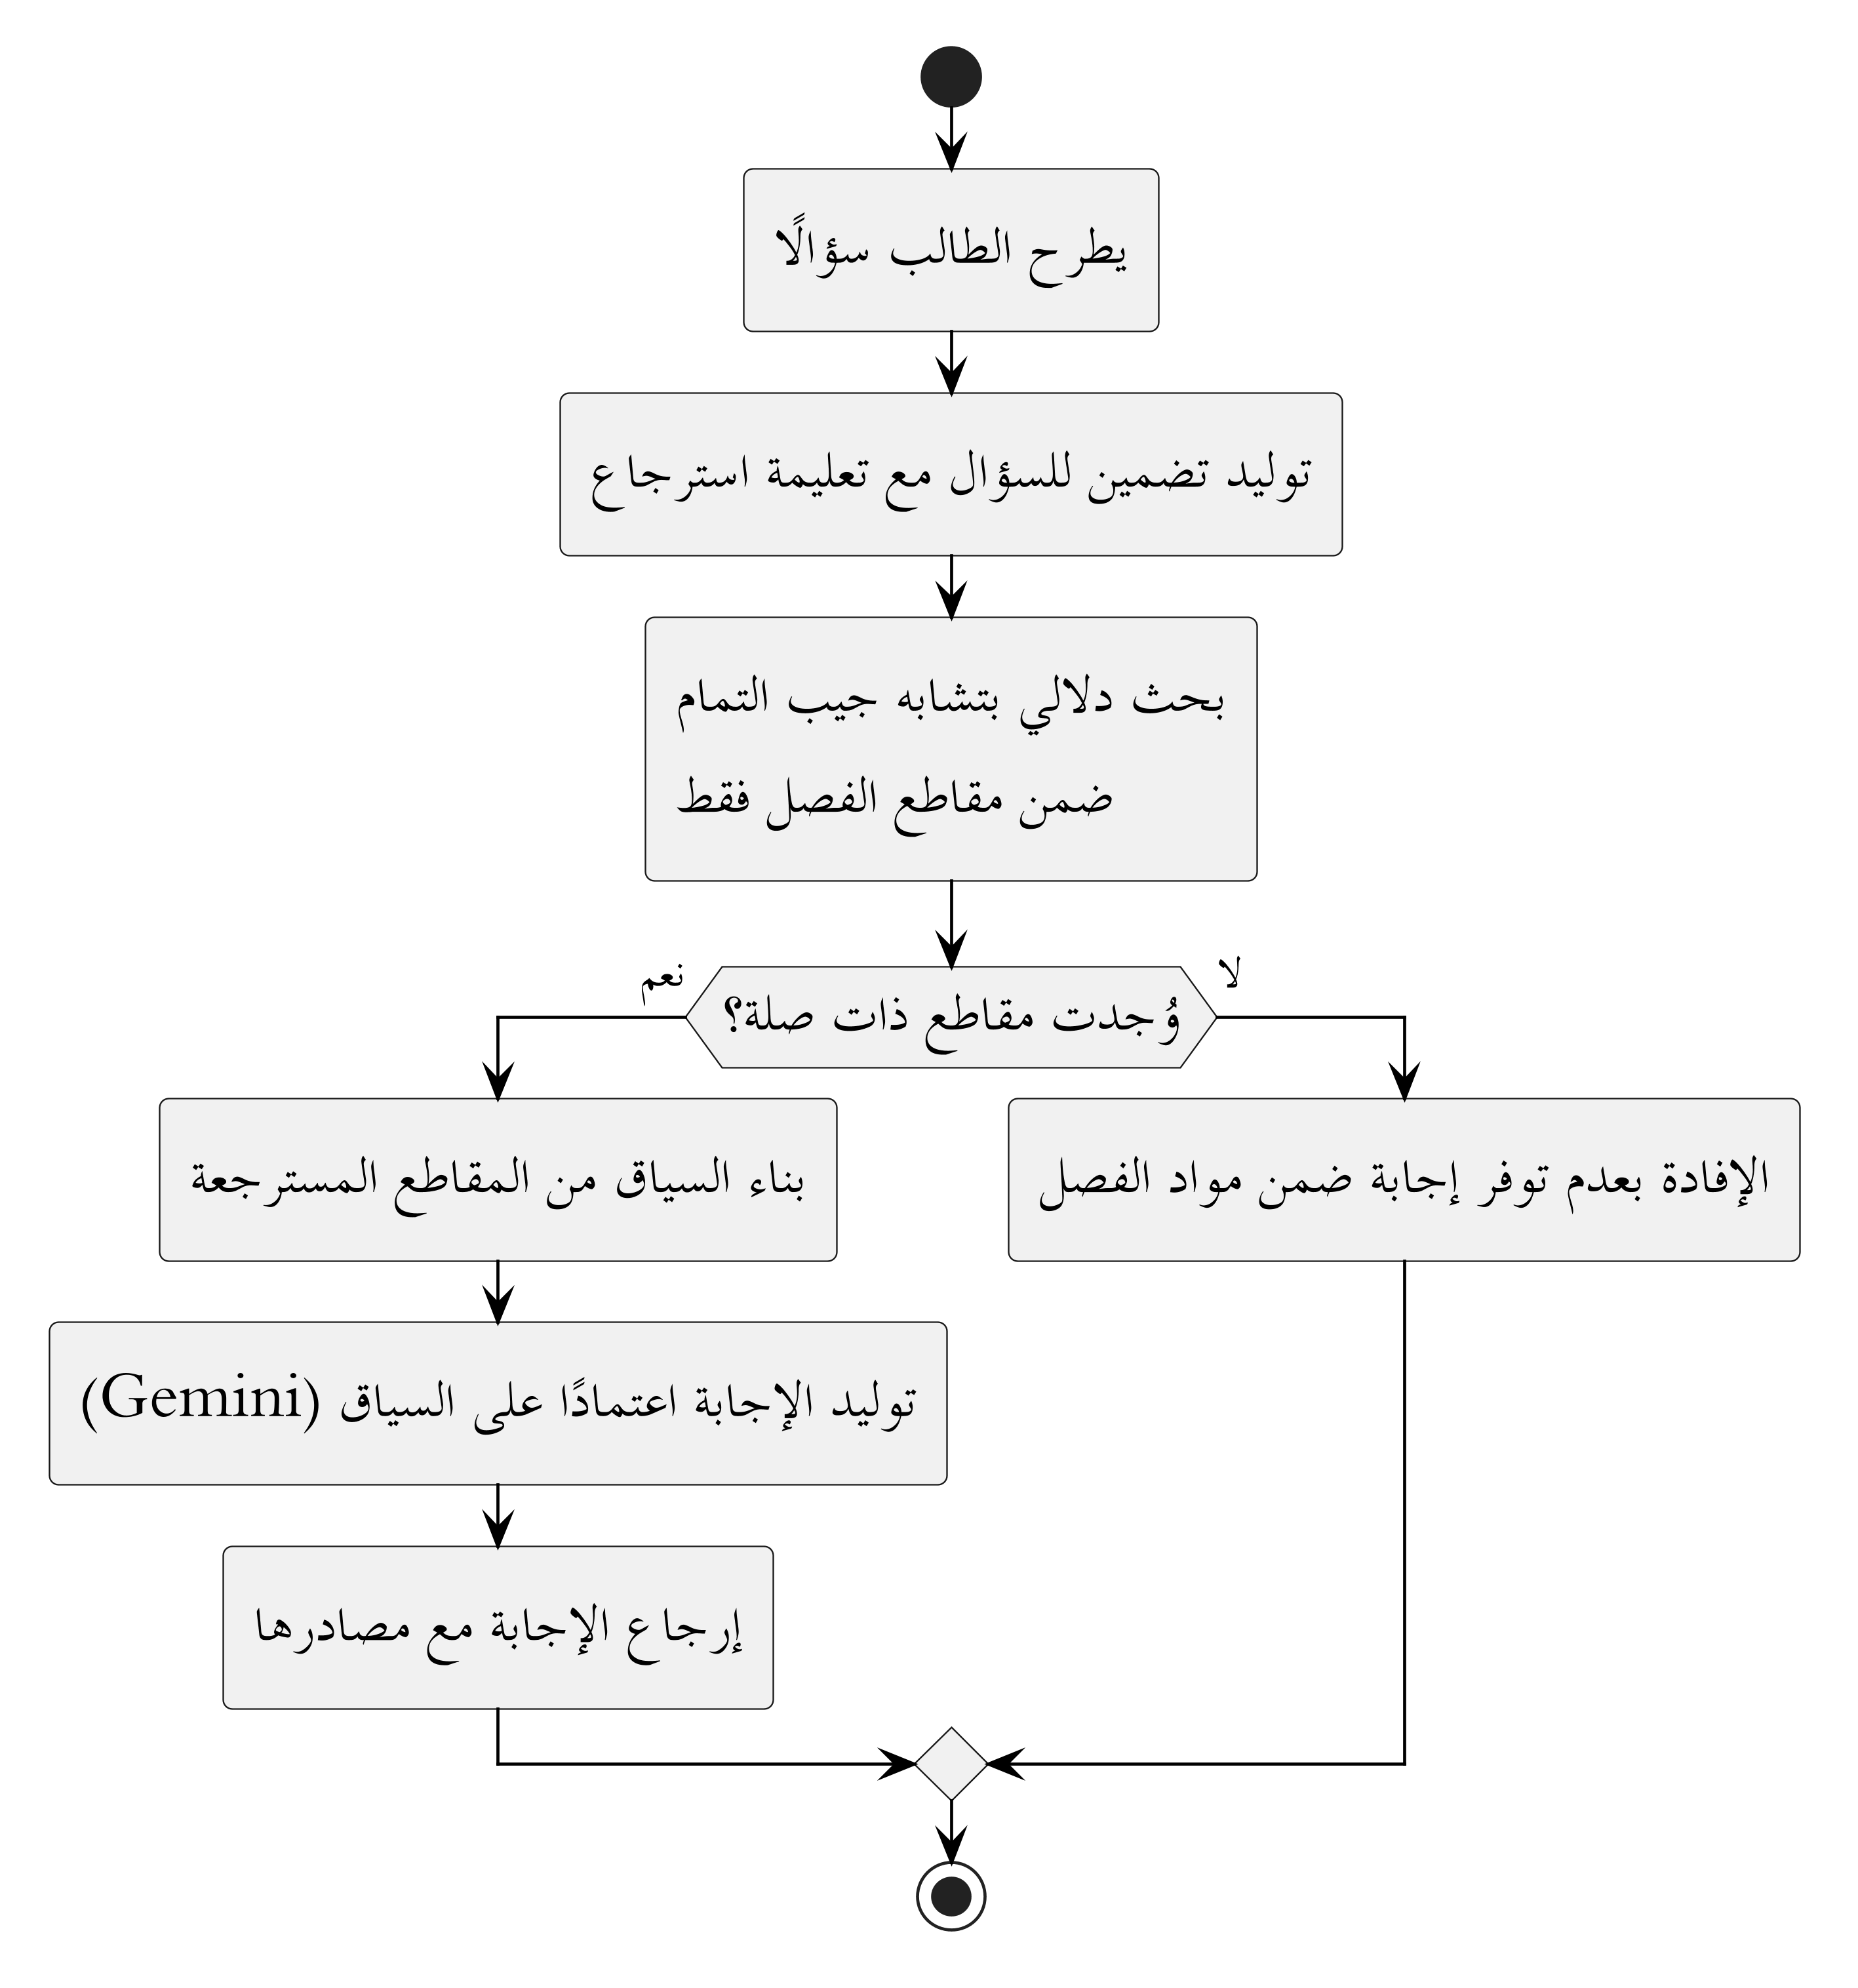
\includegraphics[width=\textwidth,height=0.8\textheight,keepaspectratio]{figures/arch-02b-rag-retrieval.png}
  \caption{تدفّق الاسترجاع وتوليد الإجابة عن سؤال الطالب.}
  \label{fig:arch-02b}
\end{figure}

\subsubsection{تدفّق توليد ملخّص الجلسة}
\label{subsubsec:flow-summary}

يبيّن الشكل~\ref{fig:arch-03b} مسار توليد ملخّص الجلسة بعد انتهائها.

\begin{figure}[htbp]
  \centering
  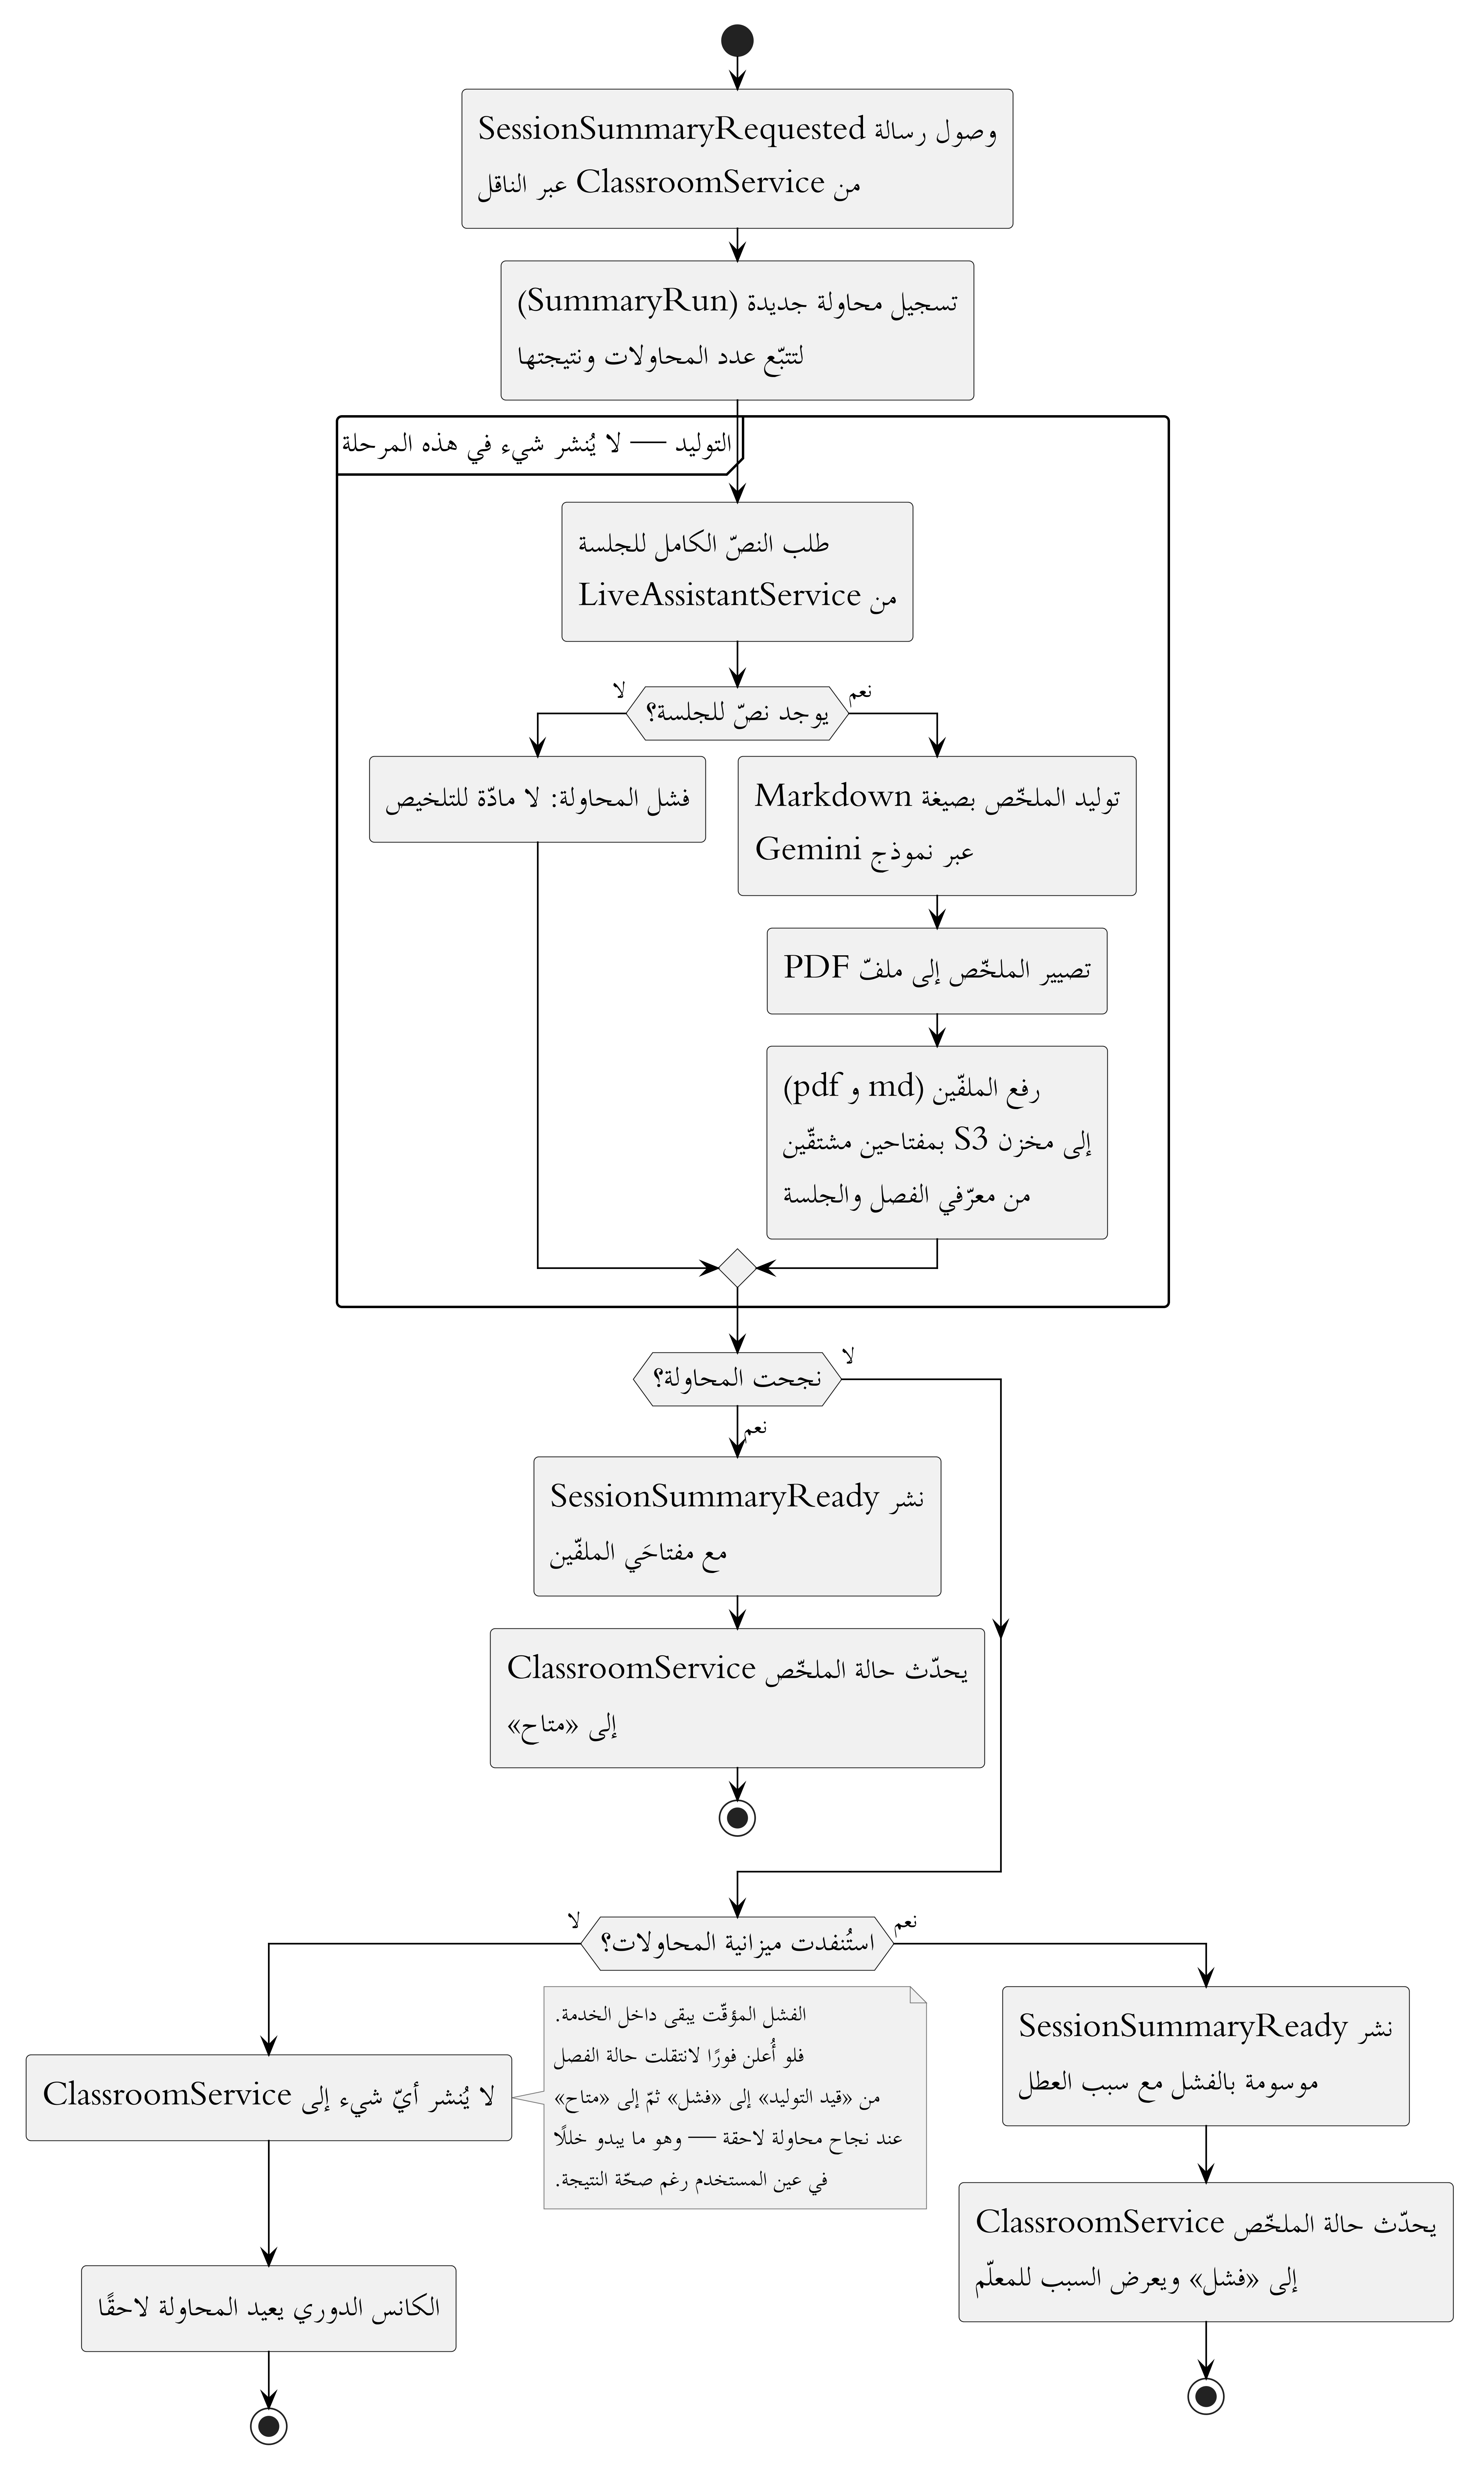
\includegraphics[width=\textwidth,height=0.8\textheight,keepaspectratio]{figures/arch-03b-session-summary.png}
  \caption{تدفّق توليد ملخّص الجلسة في خدمة الاسترجاع.}
  \label{fig:arch-03b}
\end{figure}

\noindent ويفصل هذا التدفّق بين التوليد والإعلان: فالمحاولة الفاشلة لا تنشر حدثاً ما دامت هناك محاولات باقية. ولولا هذا الفصل لانتقلت حالة الملخّص في واجهة الفصل من «قيد التوليد» إلى «فشل» ثمّ إلى «متاح» عند نجاح محاولة لاحقة، وهو تسلسل يظهر للمستخدم على أنّه خلل وإن كانت النتيجة النهائية صحيحة.

% ===========================================================================
% TODO(quiz-ssd): system sequence diagrams for the eight quiz use cases. Each
% figure block below is commented out and waiting for its PNG in figures/.
% Uncomment a block once its diagram exists — the file names are already chosen.
%   grep -n "TODO(quiz-ssd)" chapters/04-requirements-analysis.tex
% ===========================================================================
\subsection{مخطط تسلسل النظام لحالات استخدام الاختبارات}

\subsubsection{مخطط تسلسل النظام لحالة إنشاء مسودة اختبار وتوليدها}
% TODO(quiz-ssd)
\noindent [يُستكمل: مخطط تسلسل النظام لهذه الحالة.]
% \begin{figure}[htbp]
%   \centering
%   \includegraphics[width=\textwidth,height=0.8\textheight,keepaspectratio]{figures/ssd-quiz-01-compose.png}
%   \caption{مخطط تسلسل النظام لحالة «إنشاء مسودة اختبار وتوليدها».}
%   \label{fig:ssd-quiz-01}
% \end{figure}

\subsubsection{مخطط تسلسل النظام لحالة نشر الاختبار وإغلاقه أو إلغاؤه}
% TODO(quiz-ssd)
\noindent [يُستكمل: مخطط تسلسل النظام لهذه الحالة.]
% \begin{figure}[htbp]
%   \centering
%   \includegraphics[width=\textwidth,height=0.8\textheight,keepaspectratio]{figures/ssd-quiz-02-lifecycle.png}
%   \caption{مخطط تسلسل النظام لحالة «نشر الاختبار وإغلاقه أو إلغاؤه».}
%   \label{fig:ssd-quiz-02}
% \end{figure}

\subsubsection{مخطط تسلسل النظام لحالة تمديد مهلة الإجابة}
% TODO(quiz-ssd)
\noindent [يُستكمل: مخطط تسلسل النظام لهذه الحالة.]
% \begin{figure}[htbp]
%   \centering
%   \includegraphics[width=\textwidth,height=0.8\textheight,keepaspectratio]{figures/ssd-quiz-03-extend.png}
%   \caption{مخطط تسلسل النظام لحالة «تمديد مهلة الإجابة».}
%   \label{fig:ssd-quiz-03}
% \end{figure}

\subsubsection{مخطط تسلسل النظام لحالة استعراض نتائج الاختبار}
% TODO(quiz-ssd)
\noindent [يُستكمل: مخطط تسلسل النظام لهذه الحالة.]
% \begin{figure}[htbp]
%   \centering
%   \includegraphics[width=\textwidth,height=0.8\textheight,keepaspectratio]{figures/ssd-quiz-04-results.png}
%   \caption{مخطط تسلسل النظام لحالة «استعراض نتائج الاختبار».}
%   \label{fig:ssd-quiz-04}
% \end{figure}

\subsubsection{مخطط تسلسل النظام لحالة متابعة تحصيل الطلاب في الفصل الدراسي}
% TODO(quiz-ssd)
\noindent [يُستكمل: مخطط تسلسل النظام لهذه الحالة.]
% \begin{figure}[htbp]
%   \centering
%   \includegraphics[width=\textwidth,height=0.8\textheight,keepaspectratio]{figures/ssd-quiz-05-tracking.png}
%   \caption{مخطط تسلسل النظام لحالة «متابعة تحصيل الطلاب في الفصل الدراسي».}
%   \label{fig:ssd-quiz-05}
% \end{figure}

\subsubsection{مخطط تسلسل النظام لحالة الإجابة عن الاختبار وتسليمه}
% TODO(quiz-ssd)
\noindent [يُستكمل: مخطط تسلسل النظام لهذه الحالة.]
% \begin{figure}[htbp]
%   \centering
%   \includegraphics[width=\textwidth,height=0.8\textheight,keepaspectratio]{figures/ssd-quiz-06-answer.png}
%   \caption{مخطط تسلسل النظام لحالة «الإجابة عن الاختبار وتسليمه».}
%   \label{fig:ssd-quiz-06}
% \end{figure}

\subsubsection{مخطط تسلسل النظام لحالة الاطّلاع على نتيجة الاختبار}
% TODO(quiz-ssd)
\noindent [يُستكمل: مخطط تسلسل النظام لهذه الحالة.]
% \begin{figure}[htbp]
%   \centering
%   \includegraphics[width=\textwidth,height=0.8\textheight,keepaspectratio]{figures/ssd-quiz-07-my-result.png}
%   \caption{مخطط تسلسل النظام لحالة «الاطّلاع على نتيجة الاختبار».}
%   \label{fig:ssd-quiz-07}
% \end{figure}

\subsubsection{مخطط تسلسل النظام لحالة متابعة التحصيل الشخصي}
% TODO(quiz-ssd)
\noindent [يُستكمل: مخطط تسلسل النظام لهذه الحالة.]
% \begin{figure}[htbp]
%   \centering
%   \includegraphics[width=\textwidth,height=0.8\textheight,keepaspectratio]{figures/ssd-quiz-08-my-tracking.png}
%   \caption{مخطط تسلسل النظام لحالة «متابعة التحصيل الشخصي».}
%   \label{fig:ssd-quiz-08}
% \end{figure}

\chapter{تصميم النظام}

\begin{chaptersummary}
يعرض هذا الفصل تصميم النظام. يبدأ بمخطط المكوّنات العام ونمطَي الاتصال بين الخدمات، ثمّ يعرض أنماط التصميم المعتمدة ومكوّنات تطبيق الويب، ثمّ نخصص لكل خدمة قسمًا يتناول مكوّناتها التفصيلية وروابطها مع محيطها
\end{chaptersummary}

\section{المعمارية العامة}
% Content for Chapter 5, Section 5.1 — pulled in by chapters/05-system-design.tex
\subsection{لمحة عن دور كل خدمة}

يتألّف النظام من ستّ خدمات مصغّرة مستقلّة تعمل خلف بوّابة واحدة (\en{Gateway}). وتتشارك هذه الخدمات بنيةً تحتية تضمّ قواعد بيانات منفصلة وناقل رسائل (\en{Message Bus}) ومخزن ملفّات وخادم وسائط. وفيما يأتي دور كل خدمة منها:

\begin{enumerate}
  \item \textbf{خدمة إدارة المستخدمين} (\en{UserManagementService}): تتولّى الهوية والأدوار والصلاحيات. وتقوم بإصدار رموز الوصول، وتدير التسجيل والدخول واستعادة كلمة المرور، وتنفّذ العمليات الإدارية التي تمسّ بقيّة الخدمات.
  \item \textbf{خدمة الفصول الدراسية} (\en{ClassroomService}): تدير الفصول والعضوية والجلسات والاختبارات والملفّات المرجعية، إضافةً إلى مخرجات الجلسات من تسجيلات وملخّصات.
  \item \textbf{خدمة البث} (\en{StreamingService}): تدير غرف البث المباشر وصلاحيات النشر فيها، وتتولّى تسجيل الجلسات عبر \en{LiveKit Egress} وحفظها في مخزن الملفّات.
  \item \textbf{خدمة البريد} (\en{EmailService}): تتلقّى الرسائل من الناقل وترسل الإشعارات البريدية المقابلة لها.
  \item \textbf{خدمة المعرفة} (\en{RagService}): تحوّل المواد المرجعية إلى مقاطع (\en{Chunks}) قابلة للبحث الدلالي، وتخدم الاسترجاع، وتولّد ملخّصات الجلسات.
  \item \textbf{خدمة المساعد المباشر} (\en{LiveAssistantService}): تحوّل كلام الجلسة الجارية إلى نص، وتقيّم محتواه مقابل المصادر المفهرسة، وتقدّم مساعدة تعليمية مباشرة للمعلّم في أثناء الشرح.
\end{enumerate}

\subsection{مخطط مكوّنات النظام}

يعرض الشكل~\ref{fig:arch-01} هذه الخدمات مجتمعةً مع البنية التحتية والبوّابة وتطبيق الويب.

\begin{figure}[htbp]
  \centering
  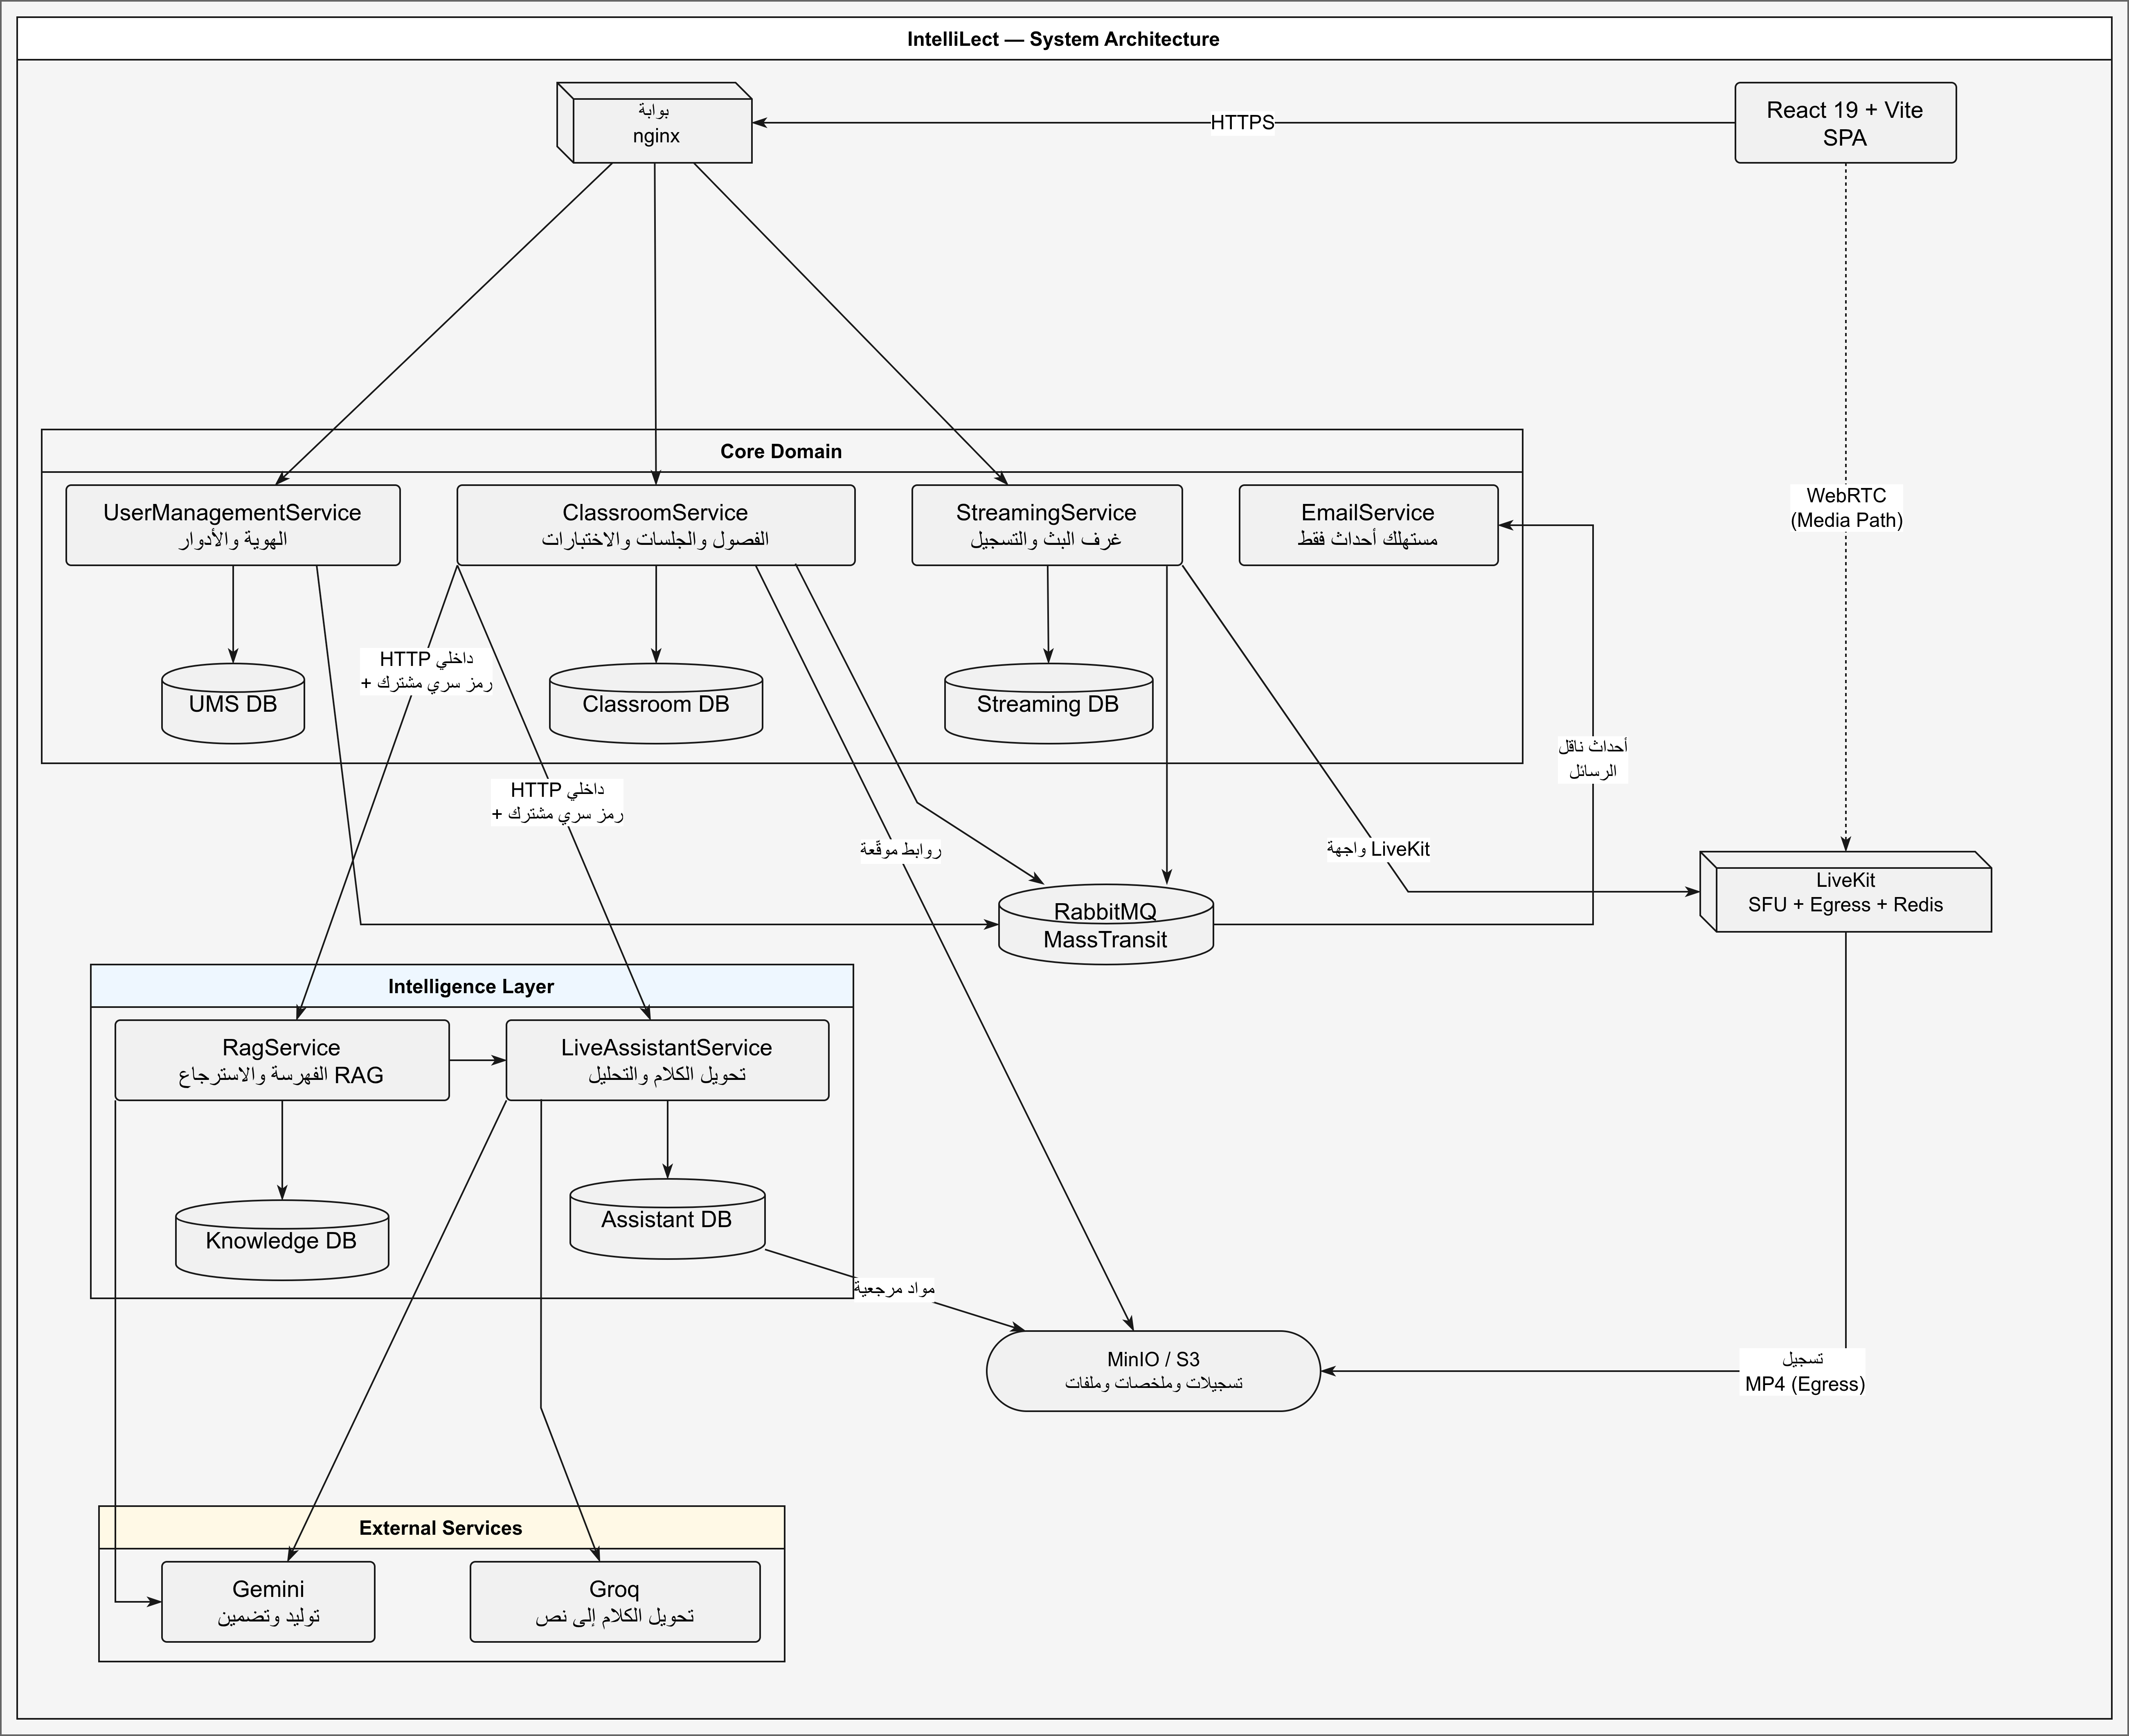
\includegraphics[width=\textwidth,height=0.8\textheight,keepaspectratio]{figures/arch-01-system-block.png}
  \caption{مخطط المكوّنات العام للنظام.}
  \label{fig:arch-01}
\end{figure}


\subsection{نمطا الاتصال بين الخدمات}

يقوم الاتصال بين الخدمات على نمطين أساسيين:

\begin{enumerate}
  \item \textbf{اتصال مباشر (متزامن) عبر \en{HTTP}}: يُستعمل حين تحتاج الخدمة إلى جواب قبل إكمال عملها. وتُعرَض هذه النقاط تحت المسار \en{/api/internal}، ولا تمرّ عبر البوّابة، ويحرسها سرٌّ مشترك يُرسَل في الترويسة \en{X-Internal-Secret}.
  \item \textbf{اتصال غير مباشر (غير متزامن) عبر ناقل الرسائل}: يُستعمل حين لا تحتاج الخدمة المرسِلة إلى جواب. ويُنفَّذ هذا النمط بالناقل \en{RabbitMQ} بوساطة \en{MassTransit}.
\end{enumerate}


\section{أنماط التصميم المعتمدة}
\label{sec:design-patterns}
% Content for Chapter 5, Section 5.2 — Design Patterns
تُعد أنماط التصميم (\en{Design Patterns}) بمثابة حلول معيارية لمشكلات هندسية متكررة في بناء الأنظمة البرمجية، حيث توفر لغة مشتركة للمطورين وتضمن استدامة الرماز المصدري. في مشروع \en{IntelliLect}، لم يكن الغرض من اعتماد هذه الأنماط مجرد الالتزام بالمعايير، بل كان الهدف الجوهري هو عزل الأجزاء المتغيرة عن الثابتة، وضمان قابلية النظام للاختبار (\en{Testability})، وتسهيل استبدال التقنيات الخارجية دون المساس بصلب منطق العمل.

يستعرض هذا القسم الأنماط الأساسية التي شكلت البنية التحتية للنظام، مع تبيان المبرر التقني لكل منها وموضع تطبيقه.

\subsection{قاعدة بيانات لكل خدمة (\en{Database per Service})}

يقضي هذا النمط بأن تمتلك كل خدمة مصغرة قاعدة بيانات خاصة بها حصرياً، بحيث يمتنع على أي خدمة أخرى الوصول إلى جداولها مباشرة. يعرض الشكل~\ref{fig:pattern-01} هذا المفهوم مطبّقاً على خدمتين من خدمات النظام.

\begin{figure}[htbp]
  \centering
  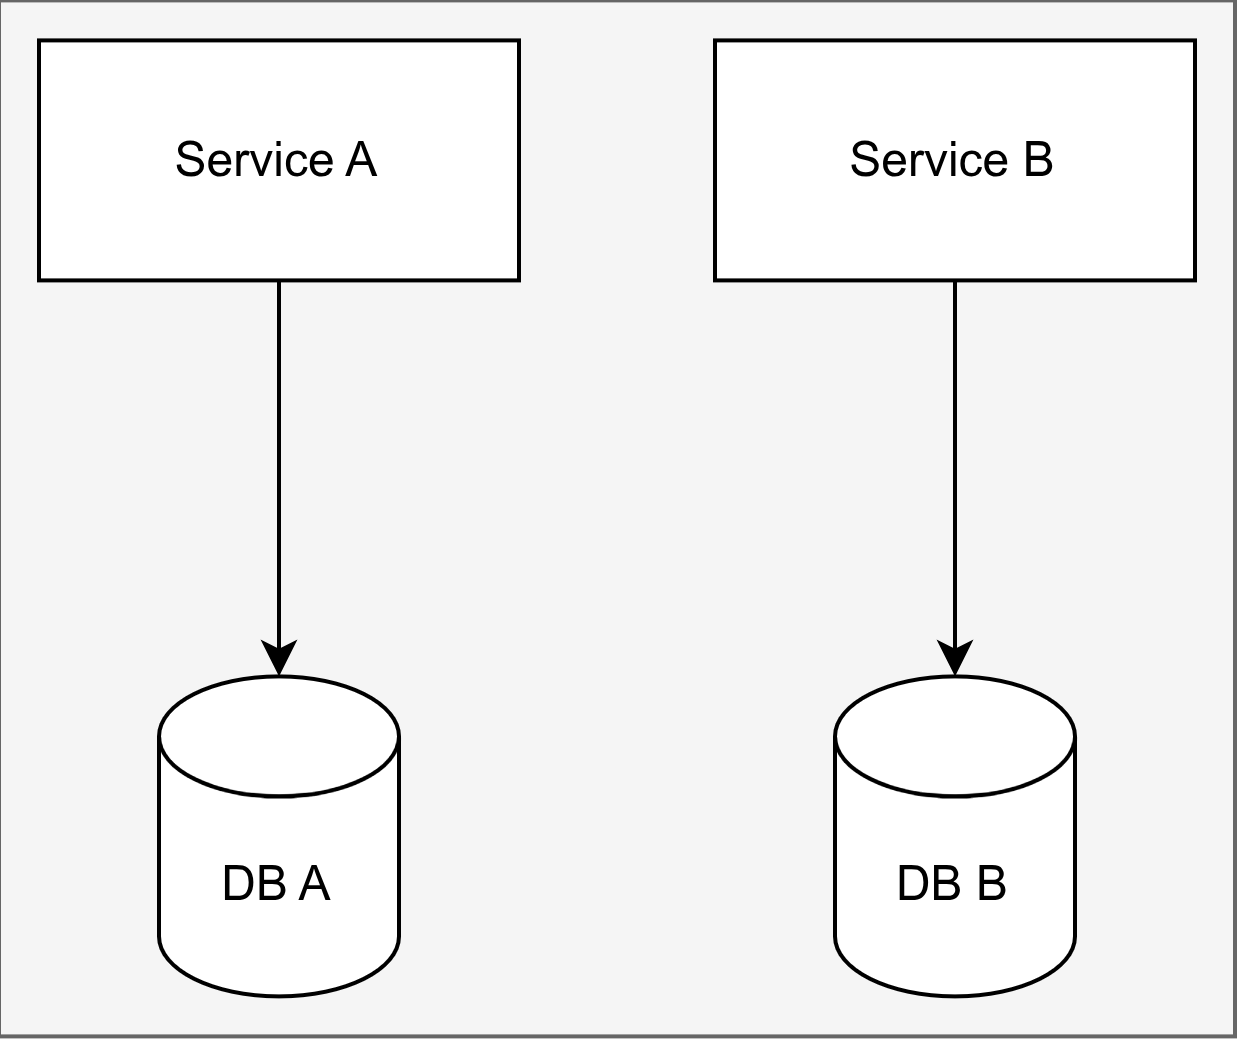
\includegraphics[width=\textwidth,height=0.8\textheight,keepaspectratio]{figures/pattern-01-database-per-service.png}
  \caption{نمط قاعدة بيانات لكل خدمة: تملك كل خدمة قاعدتها، والوصول المتقاطع ممنوع.}
  \label{fig:pattern-01}
\end{figure}

تكمن الغاية من هذا النمط في كسر الارتباط (\en{Coupling}) الذي قد ينشأ نتيجة مشاركة المخططات (\en{Schemas})؛ فحين تشترك خدمتان في قاعدة بيانات واحدة، يصبح أي تعديل في هيكلية الجداول بمثابة تغيير في "عقد ضمني" قد يؤدي إلى تعطل خدمات أخرى دون سابق إنذار. 

بناءً على هذا الأساس، تم تقسيم النظام إلى خمس قواعد بيانات منفصلة: \code{users\_db}، \code{classroomdb}، \code{streaming\_db}، \code{knowledgedb}، و\code{liveassistantdb}. وبالرغم من أن هذا الفصل استلزم استبدال الاستعلامات المباشرة (\en{Joins}) بنداءات بينية بين الخدمات، إلا أنه منحنا مرونة كاملة في تعديل وتوسيع كل خدمة بشكل مستقل.

\subsection{المنافذ والمحوِّلات (\en{Ports and Adapters})}

يهدف هذا النمط (المعروف أيضاً بالمعمارية السداسية) إلى فصل منطق التطبيق عن التفاصيل التقنية للوكلاء الخارجيين. يتم تعريف واجهات مجردة في طبقة التطبيق تسمى "المنافذ"، تصف الاحتياجات الوظيفية، بينما تتولى طبقة البنية التحتية توفير "المحوِّلات" التي تحقق هذه الواجهات. يوضح الشكل~\ref{fig:pattern-02} تطبيق هذا النمط في خدمة المعرفة.

\begin{figure}[htbp]
  \centering
  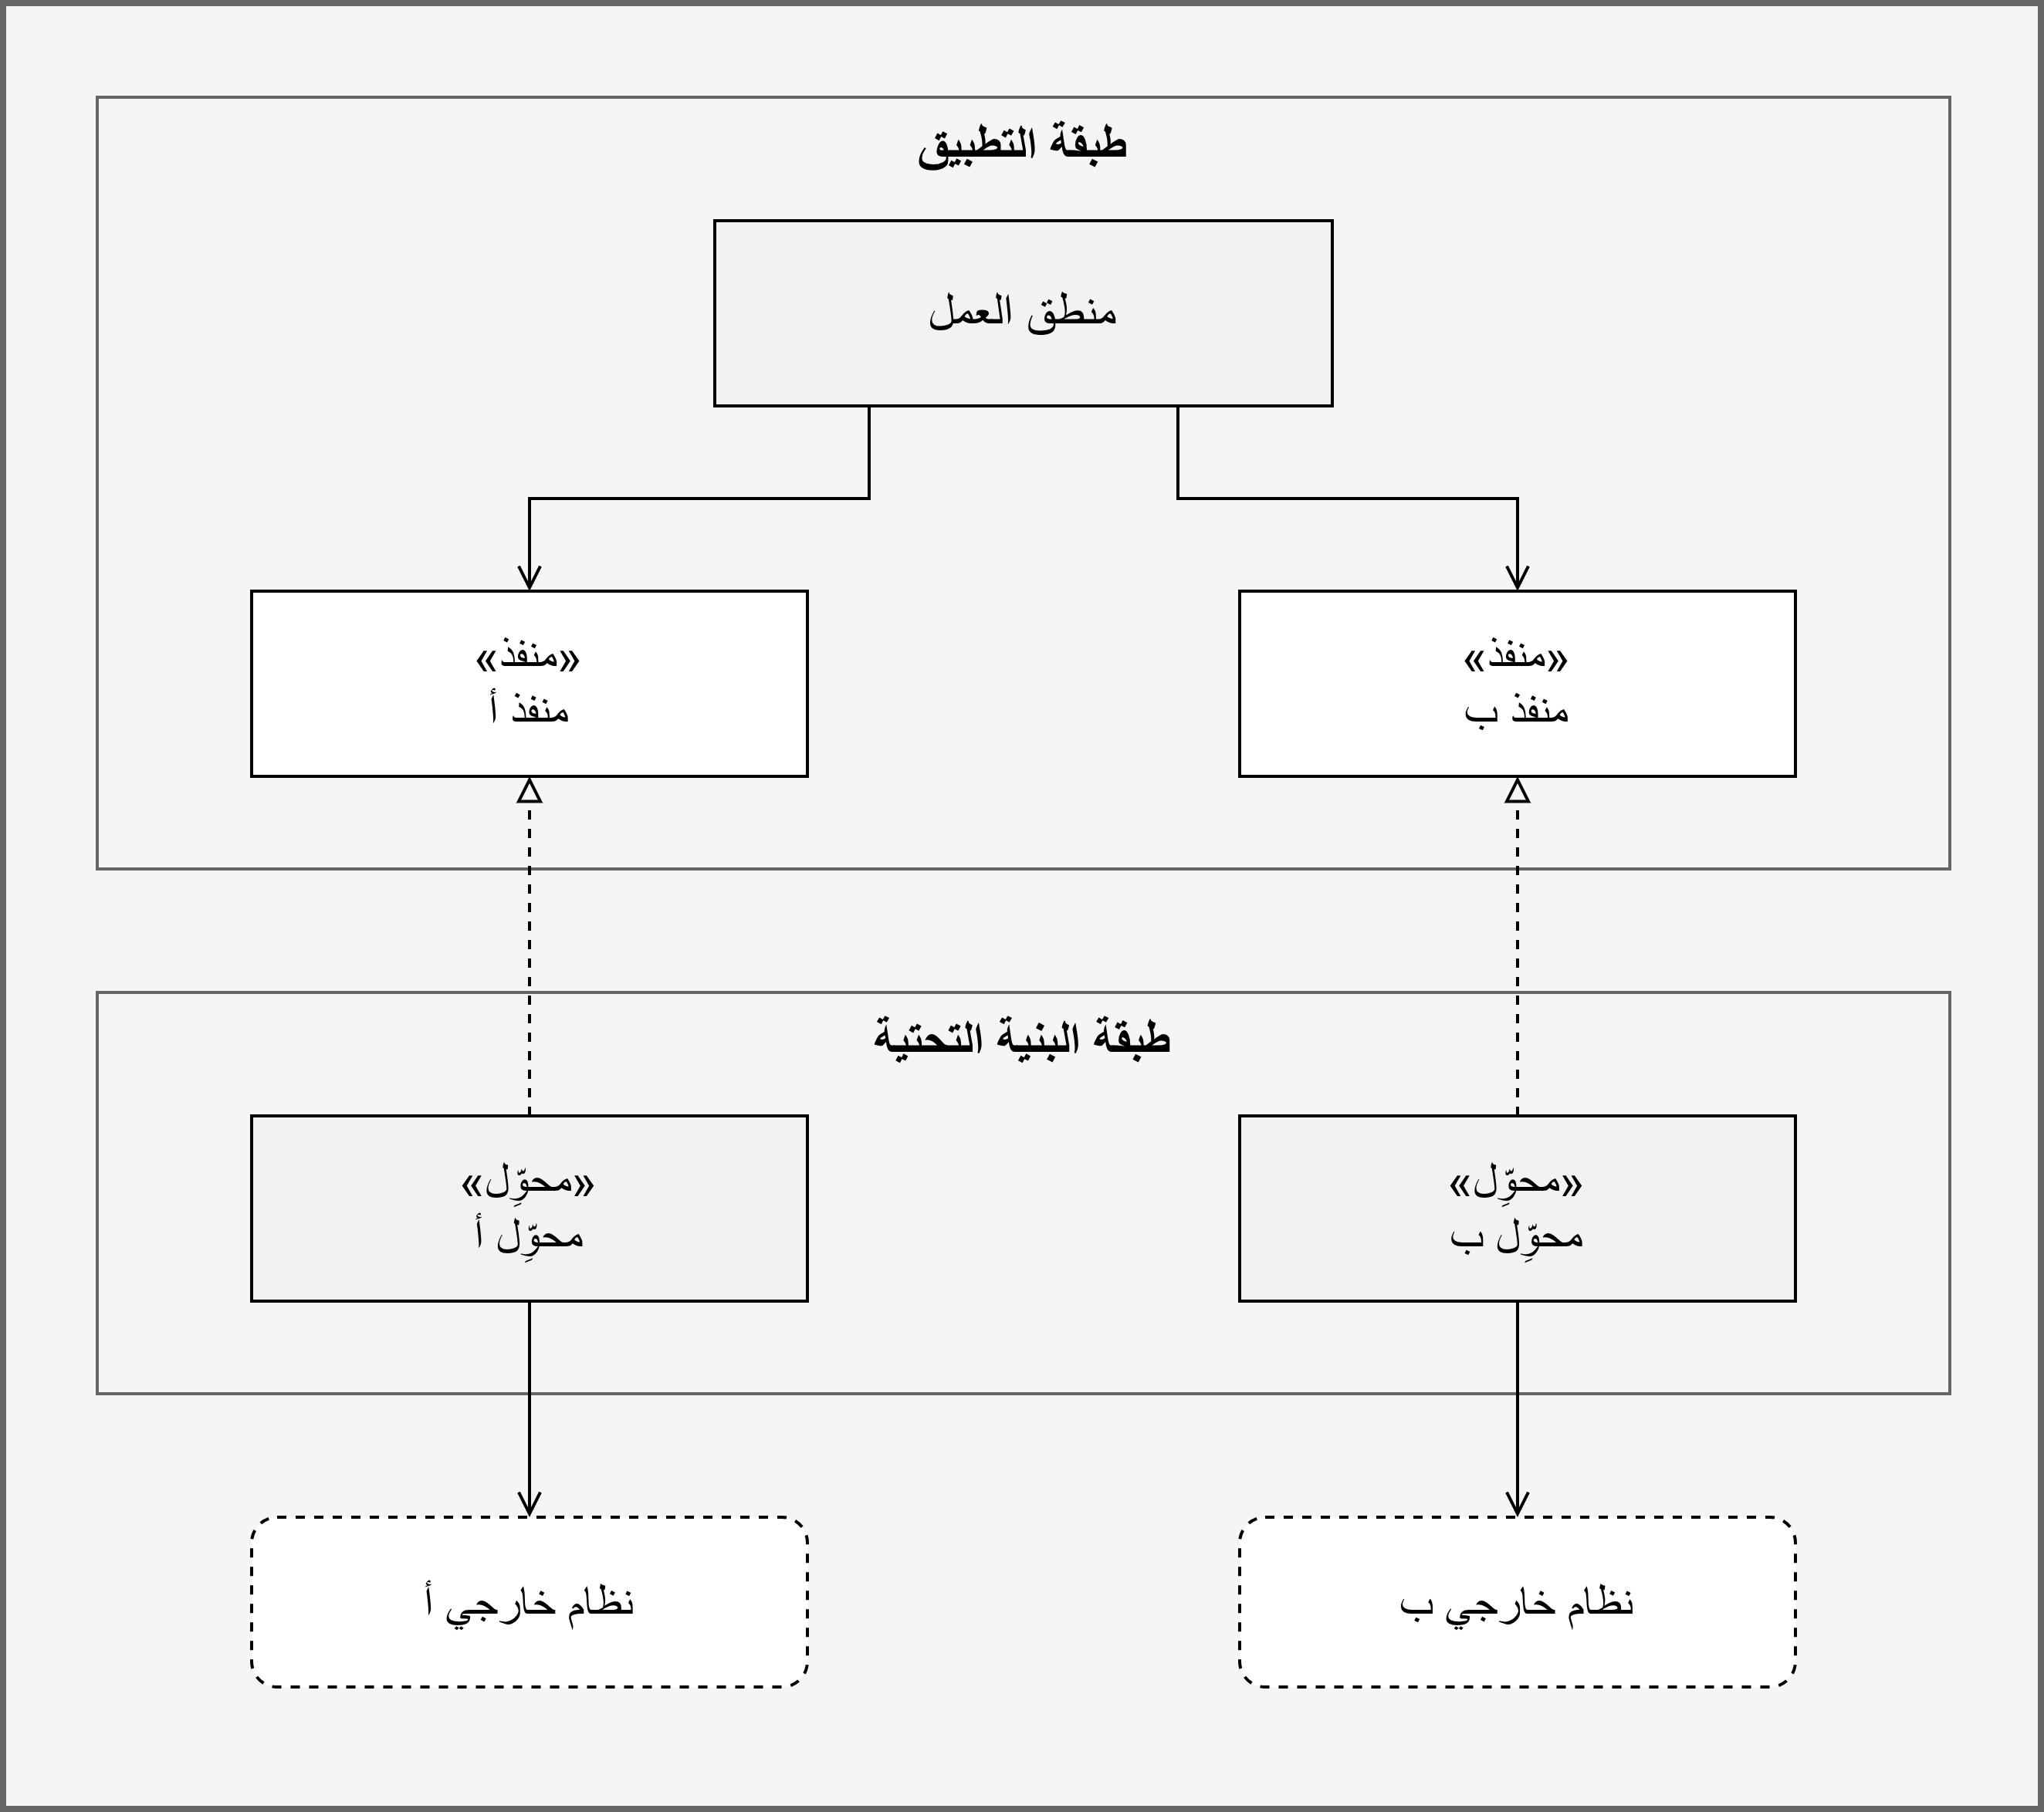
\includegraphics[width=\textwidth,height=0.8\textheight,keepaspectratio]{figures/pattern-02-ports-adapters.png}
  \caption{نمط المنافذ والمحوِّلات: المنفذ يُعرَّف في طبقة التطبيق، والمحوِّل يحقّقه في طبقة البنية التحتية.}
  \label{fig:pattern-02}
\end{figure}

يعالج هذا النمط مشكلة التبعية للتقنيات الخارجية؛ فبدلاً من أن يرتبط منطق العمل بمزود خدمة معين، تصبح الطبقة الداخلية هي التي تملي ما تحتاجه، والخارجية هي التي تلبي ذلك. وقد تم تعريف 14 منفذاً في خدمة المعرفة و8 في خدمة المساعد الحي، مما أتاح لنا اختبار المنطق البرمجي بمعزل عن قواعد البيانات أو خوادم الويب.

\subsection{الاستراتيجية (\en{Strategy})}

يعتمد هذا النمط على تعريف عائلة من الخوارزميات وجعلها قابلة للاستبدال عبر واجهة موحدة، بحيث يمكن للمستدعي استخدام أي منها دون معرفة تفاصيل تنفيذها. يوضح الشكل~\ref{fig:pattern-03} استراتيجيات تحويل الكلام إلى نص (\en{STT}).

\begin{figure}[htbp]
  \centering
  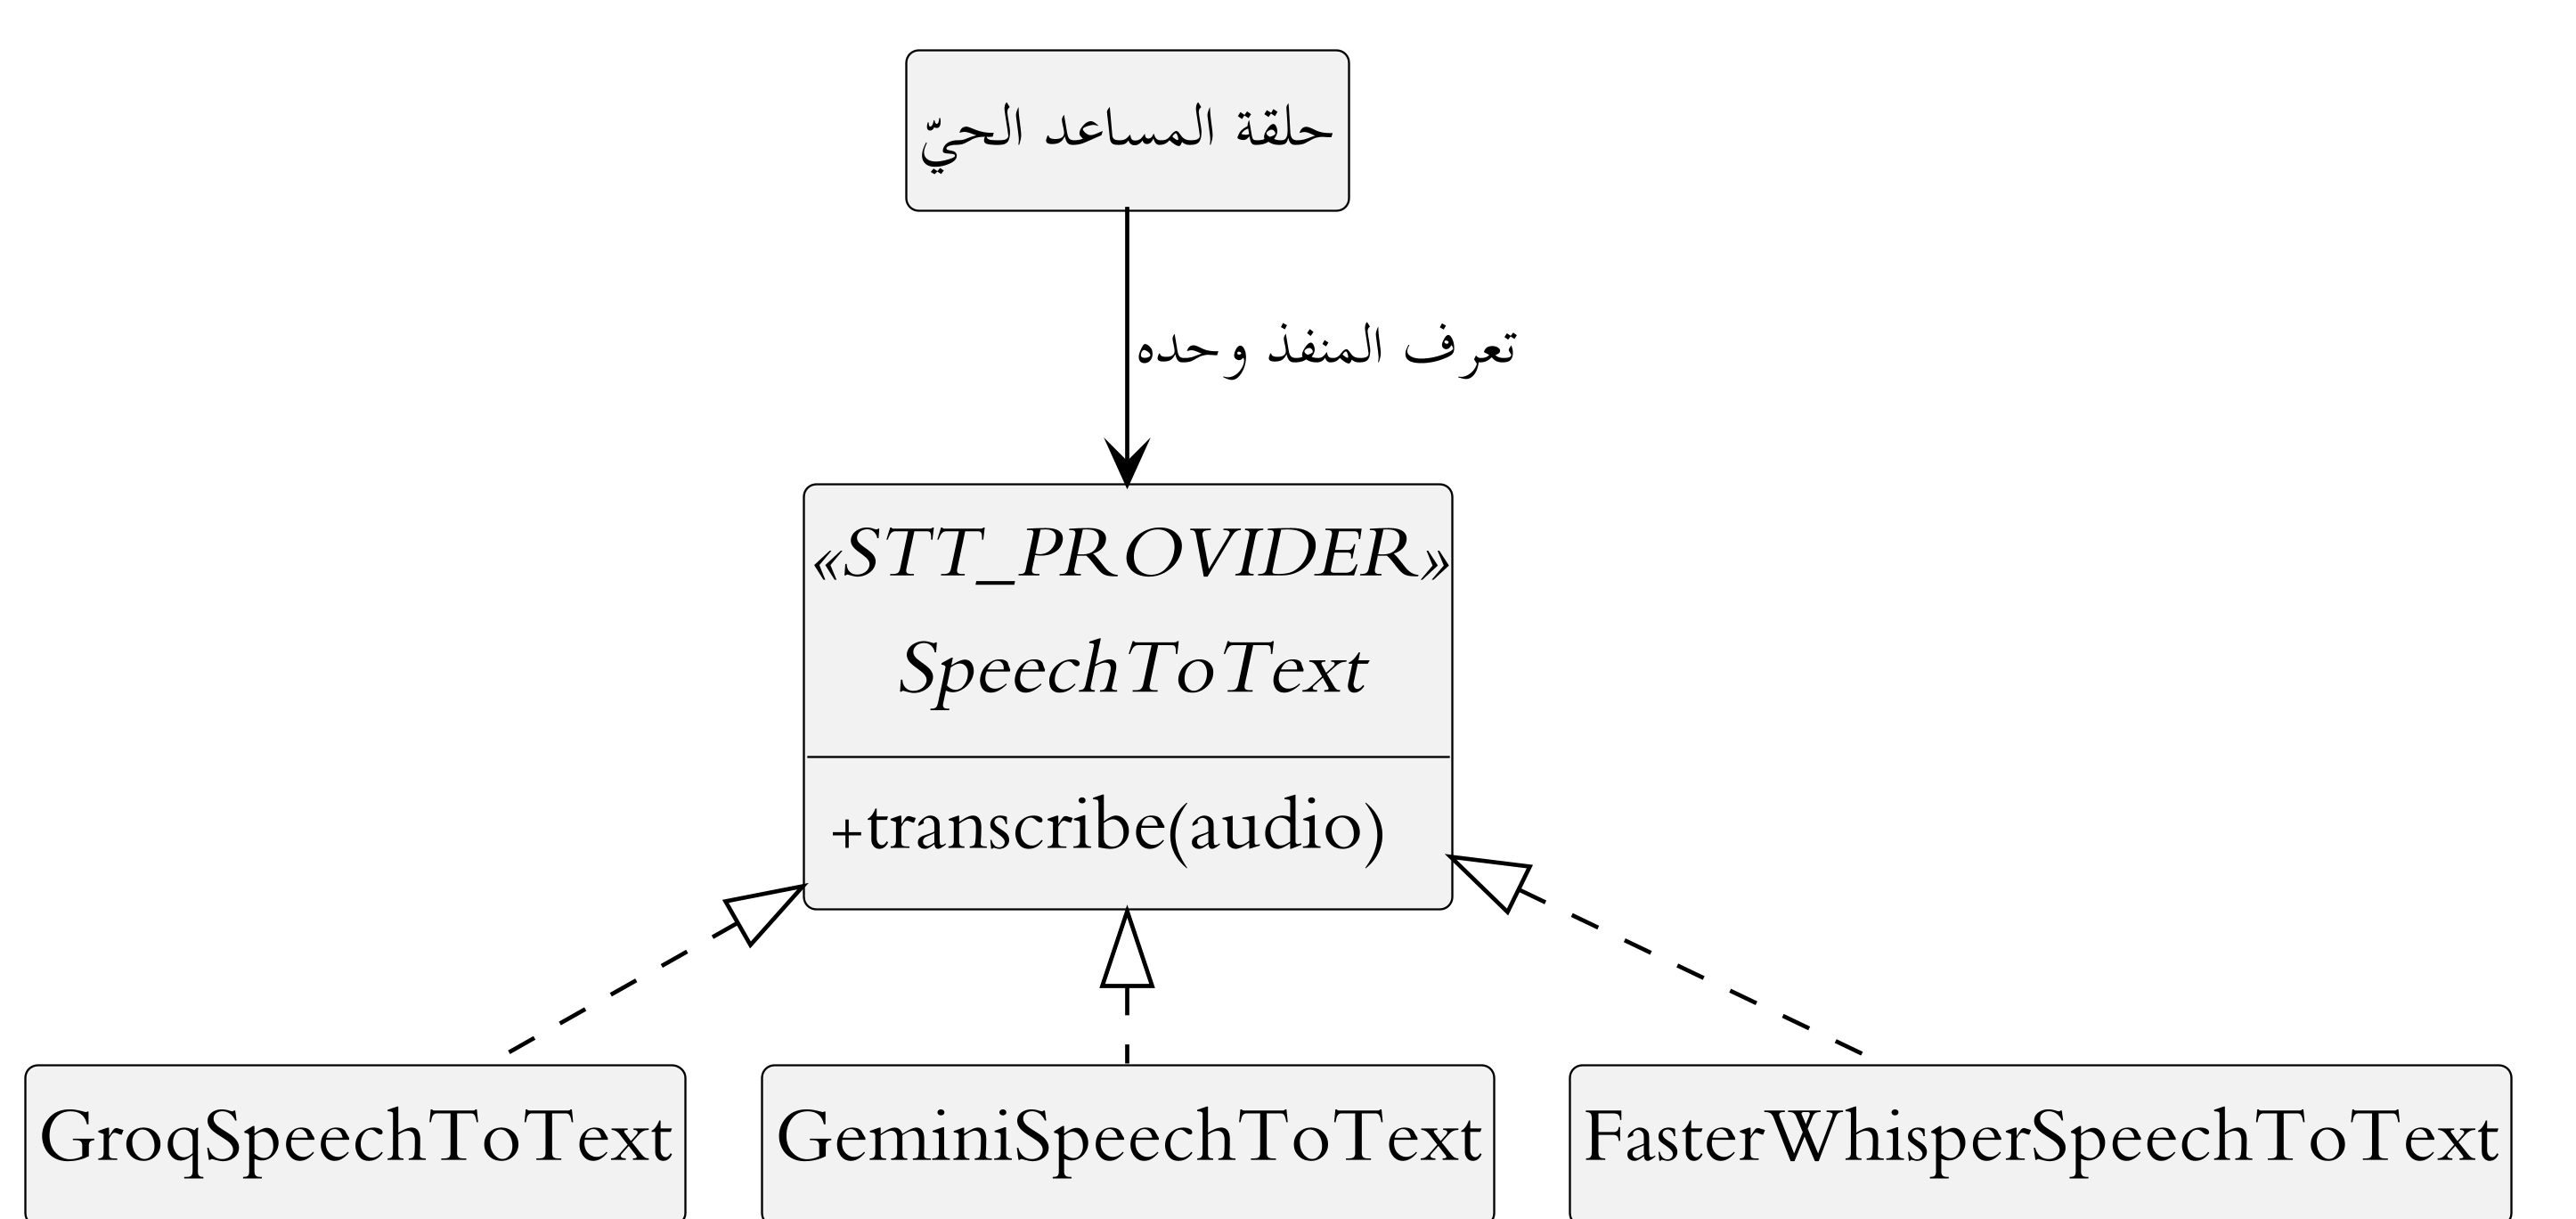
\includegraphics[width=\textwidth,height=0.8\textheight,keepaspectratio]{figures/pattern-03-strategy.png}
  \caption{نمط الاستراتيجية: منفذٌ واحد وثلاثة تحقيقات متكافئة، والمستدعي لا يعرف إلّا المنفذ.}
  \label{fig:pattern-03}
\end{figure}

استُخدم هذا النمط في المواضع التي تتطلب مفاضلة بين بدائل تقنية؛ مثل اختيار نموذج التضمين (\en{Embedding}) أو محرك تحويل الكلام. بفضل هذا النمط، أمكننا الانتقال من النماذج المحلية إلى المستضافة (مثل \en{Gemini}) أو العكس عبر تغيير بسيط في الإعدادات، دون تعديل شيفرة منطق العمل الأساسية.

\subsection{المصنع (\en{Factory})}

يعمل نمط المصنع كمتمم لنمط الاستراتيجية، حيث يتولى مسؤولية اختيار الاستراتيجية المناسبة وإنشائها بناءً على الحالة الراهنة أو الإعدادات، حاجباً بذلك منطق الاختيار عن المستهلك. يعرض الشكل~\ref{fig:pattern-04} مصنع المقسِّمات (\en{Chunkers}) في خدمة المعرفة.

\begin{figure}[htbp]
  \centering
  % Narrower than the rest on purpose: five boxes in four ranks come out taller
  % than wide, and at full width the figure fills the page and floats alone.
  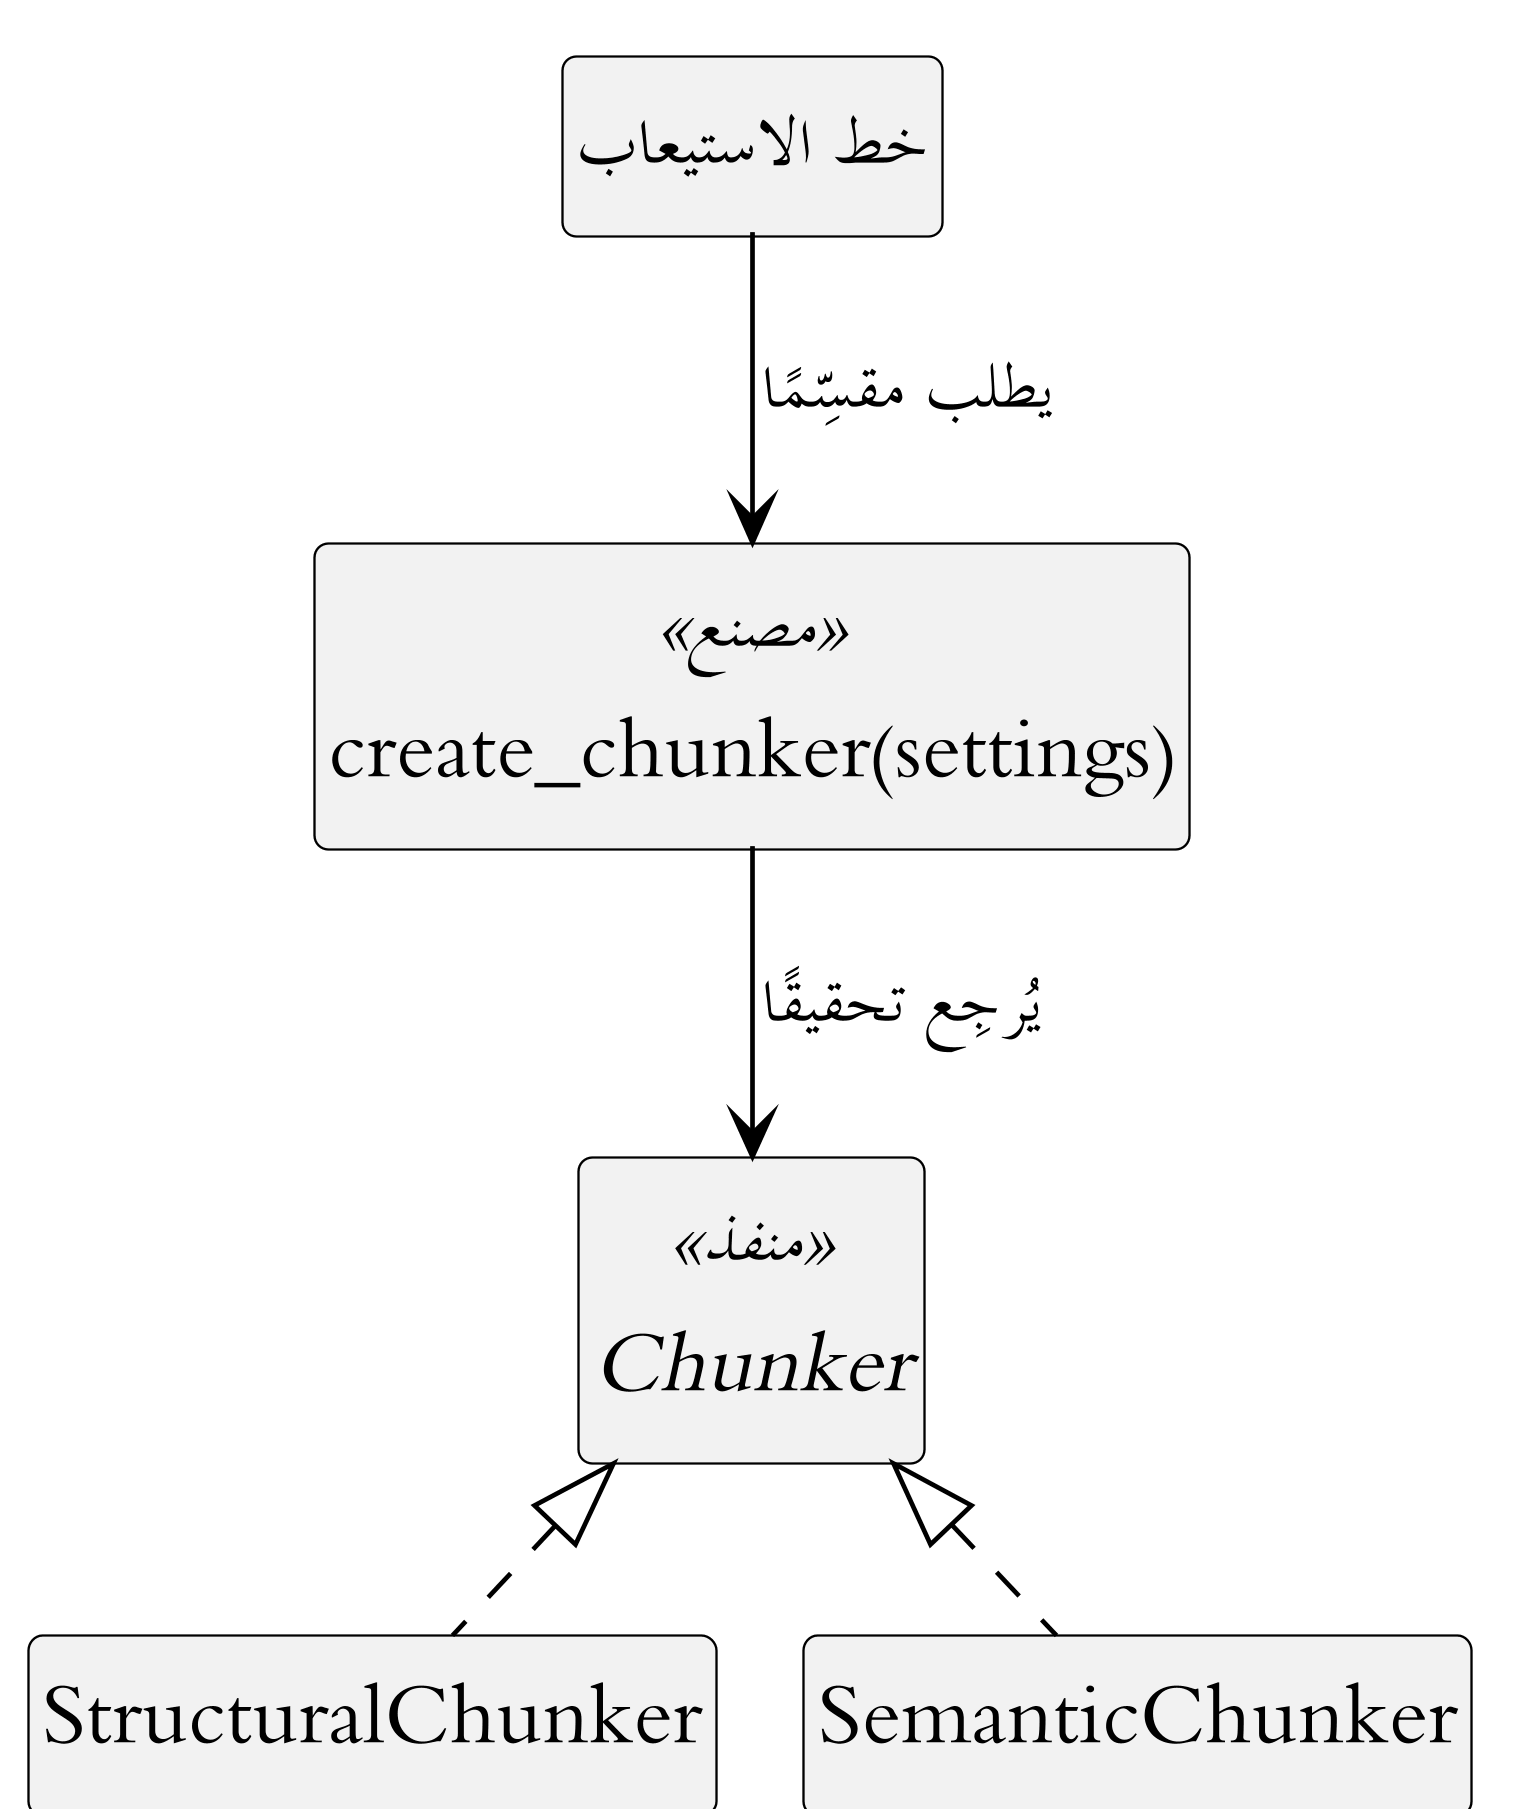
\includegraphics[width=0.6\textwidth,height=0.8\textheight,keepaspectratio]{figures/pattern-04-factory.png}
  \caption{نمط المصنع: المستدعي يطلب مقسِّمًا فيتلقّى تحقيقًا للمنفذ، دون أن يعرف أيَّها.}
  \label{fig:pattern-04}
\end{figure}

في نظامنا، نجد تطبيقات عديدة لهذا النمط، مثل \code{create\_chunker} الذي يقرأ إعدادات التقطيع ويُرجع الاستراتيجية الموافقة، و\code{ExtractorRouter} الذي يحدد المستخرج المناسب حسب نوع الملف المرفوع، مما يضمن بقاء منطق الاستدعاء بسيطاً ومركزاً على المهمة الوظيفية.

\subsection{المستودع (\en{Repository})}

يحجب نمط المستودع آليات الوصول إلى البيانات (مثل استعلامات \en{SQL} أو \en{ORM}) خلف واجهة تتحدث بلغة "المجال التعليمي". يعرض الشكل~\ref{fig:pattern-05} تحقيق هذا النمط في خدمات \en{.NET} عبر قاعدة بيانات عامة.

\begin{figure}[htbp]
  \centering
  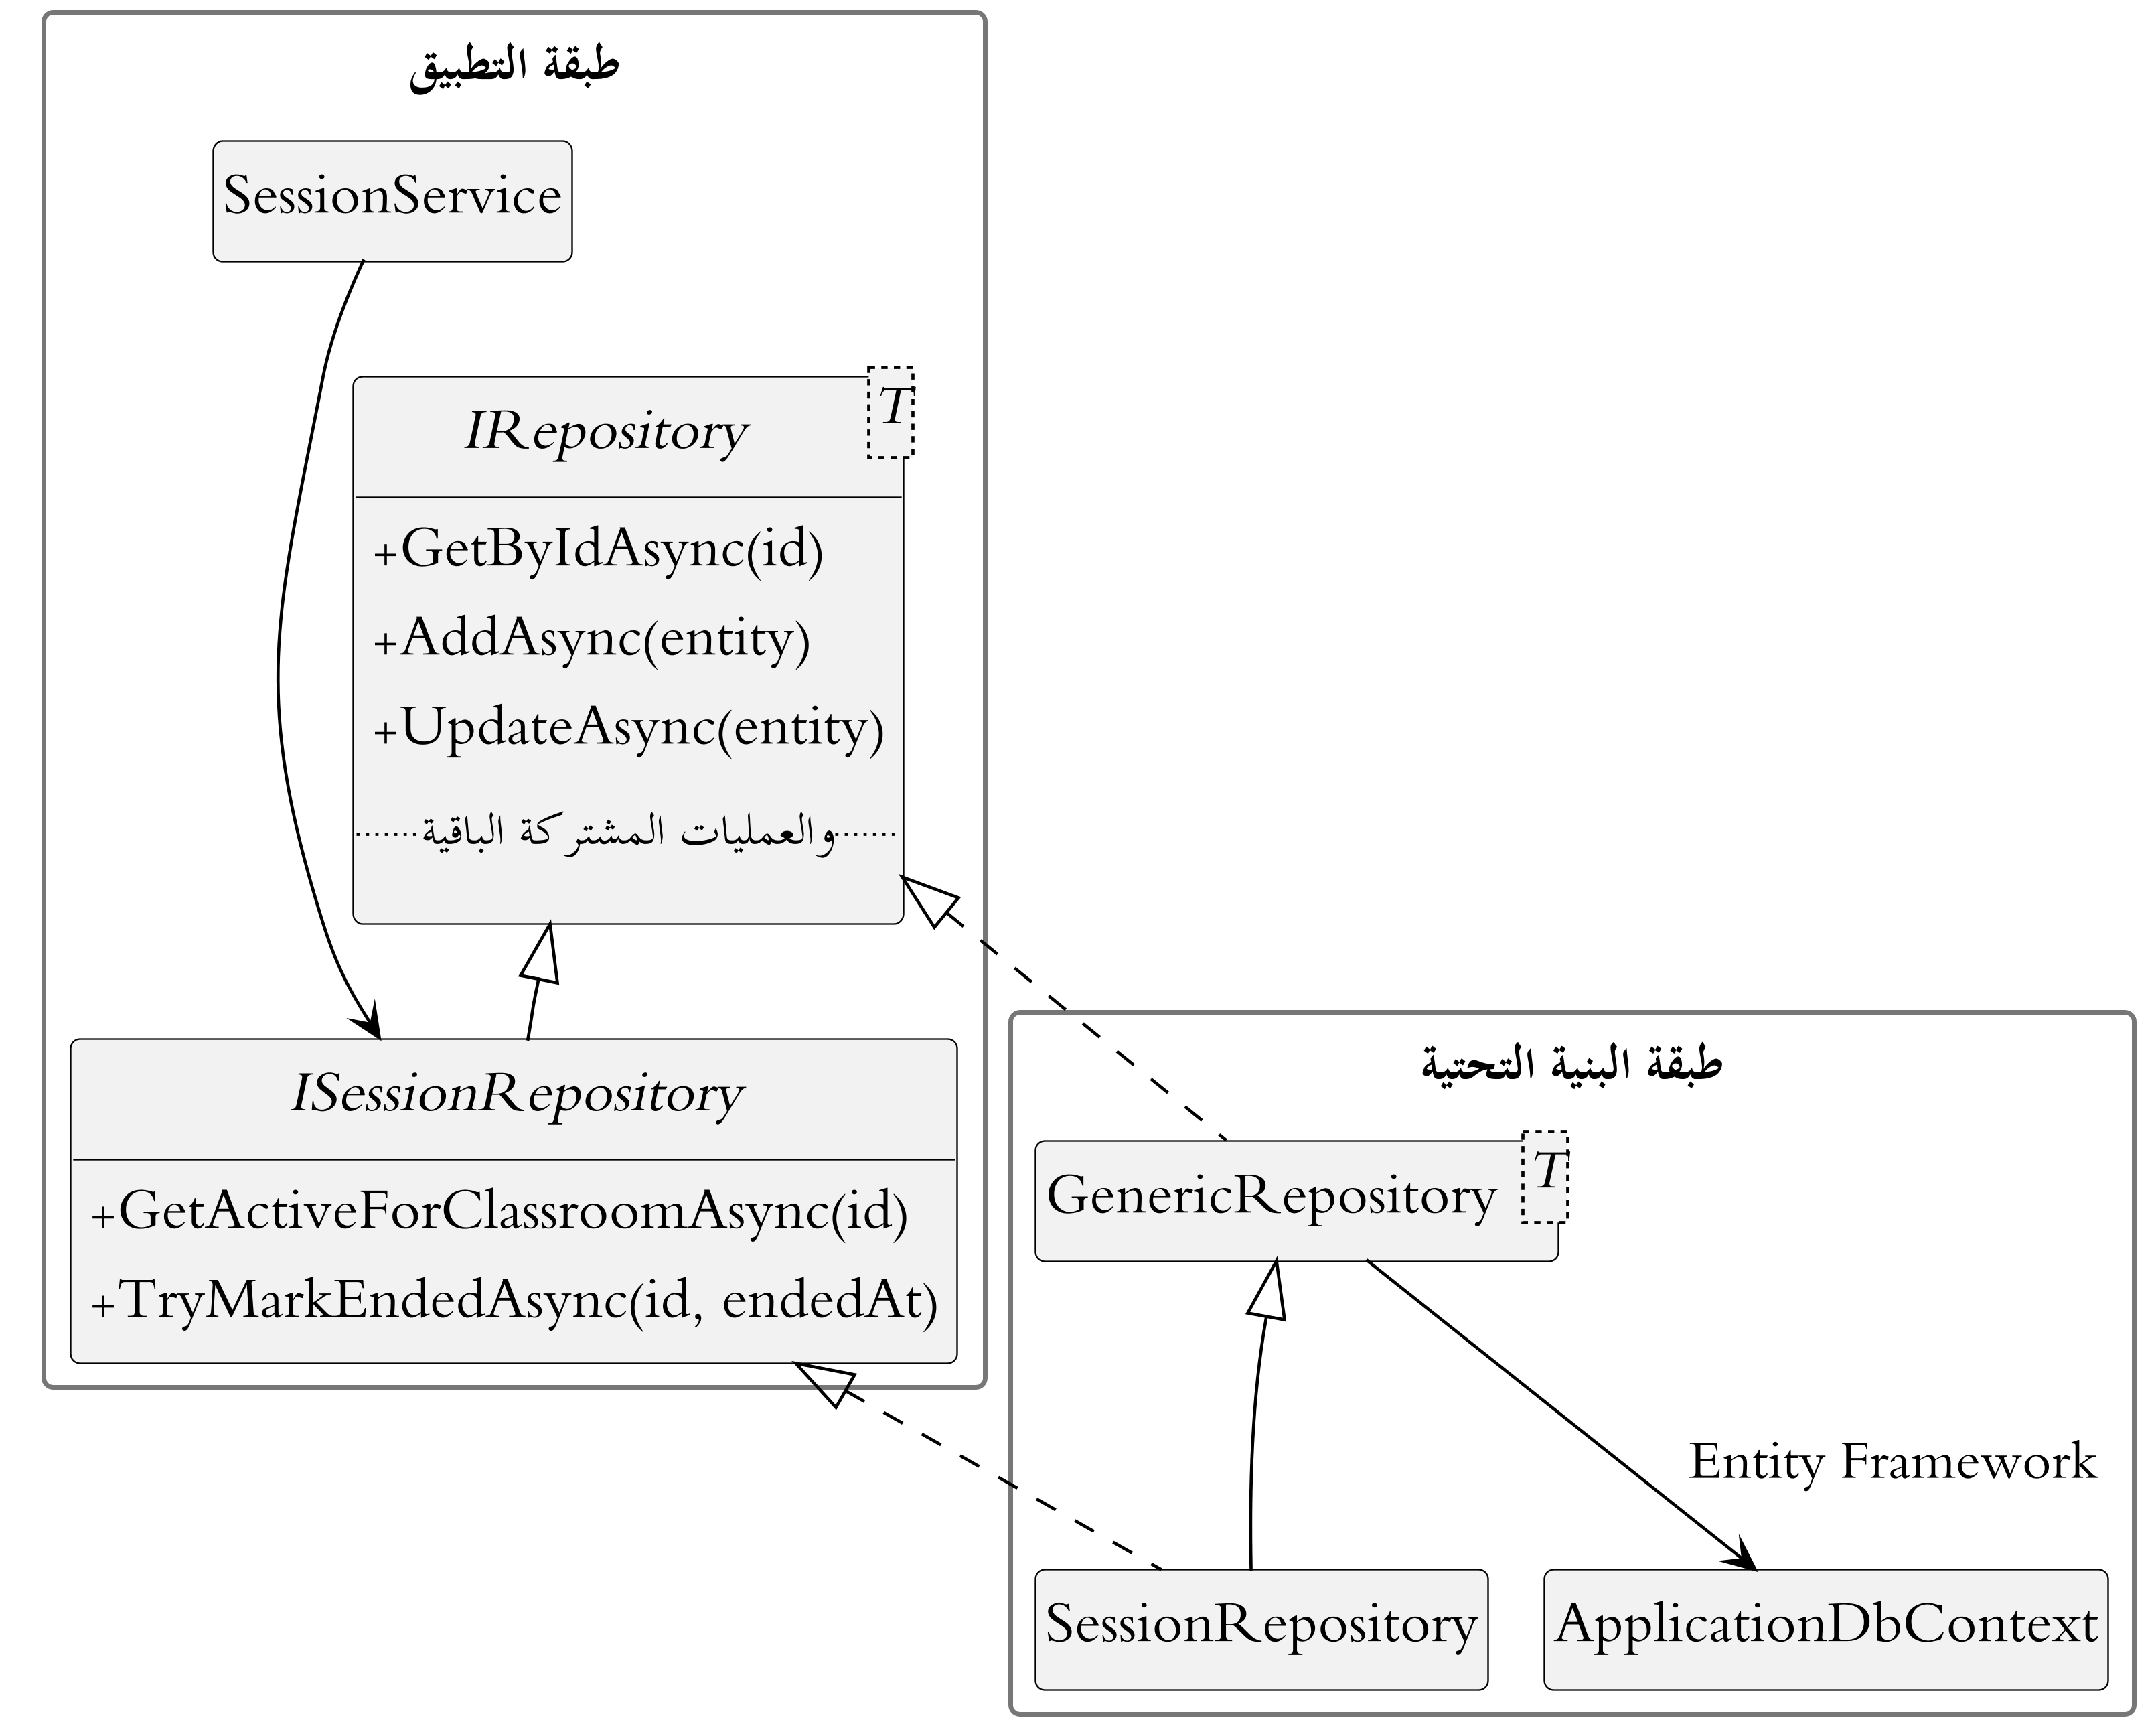
\includegraphics[width=\textwidth,height=0.8\textheight,keepaspectratio]{figures/pattern-05-repository.png}
  \caption{نمط المستودع بقاعدة عامّة: تُعرَّف الواجهة في طبقة التطبيق وتُحقَّق في طبقة البنية التحتية.}
  \label{fig:pattern-05}
\end{figure}

تكمن ميزة هذا النمط في عزل طبقة التطبيق عن مكتبات الوصول إلى البيانات مثل \en{Entity Framework}. وقد اعتمدنا مستودعاً عاماً \code{GenericRepository<T>} يحمل العمليات المتكررة، ورثته عشرة مستودعات متخصصة، مما مكننا من إجراء الاختبارات الوحدوية باستخدام مستودعات وهمية تعمل في الذاكرة دون الحاجة لقاعدة بيانات حقيقية.

\subsection{وحدة العمل (\en{Unit of Work})}

يضمن نمط وحدة العمل جمع عدة عمليات كتابة ضمن معاملة واحدة (\en{Transaction})، بحيث تنجح جميعها معاً أو تُلغى جميعاً، مما يحافظ على اتساق البيانات. يوضح الشكل~\ref{fig:pattern-06} مسار إنهاء الجلسة كمثال على هذا النمط.

\begin{figure}[htbp]
  \centering
  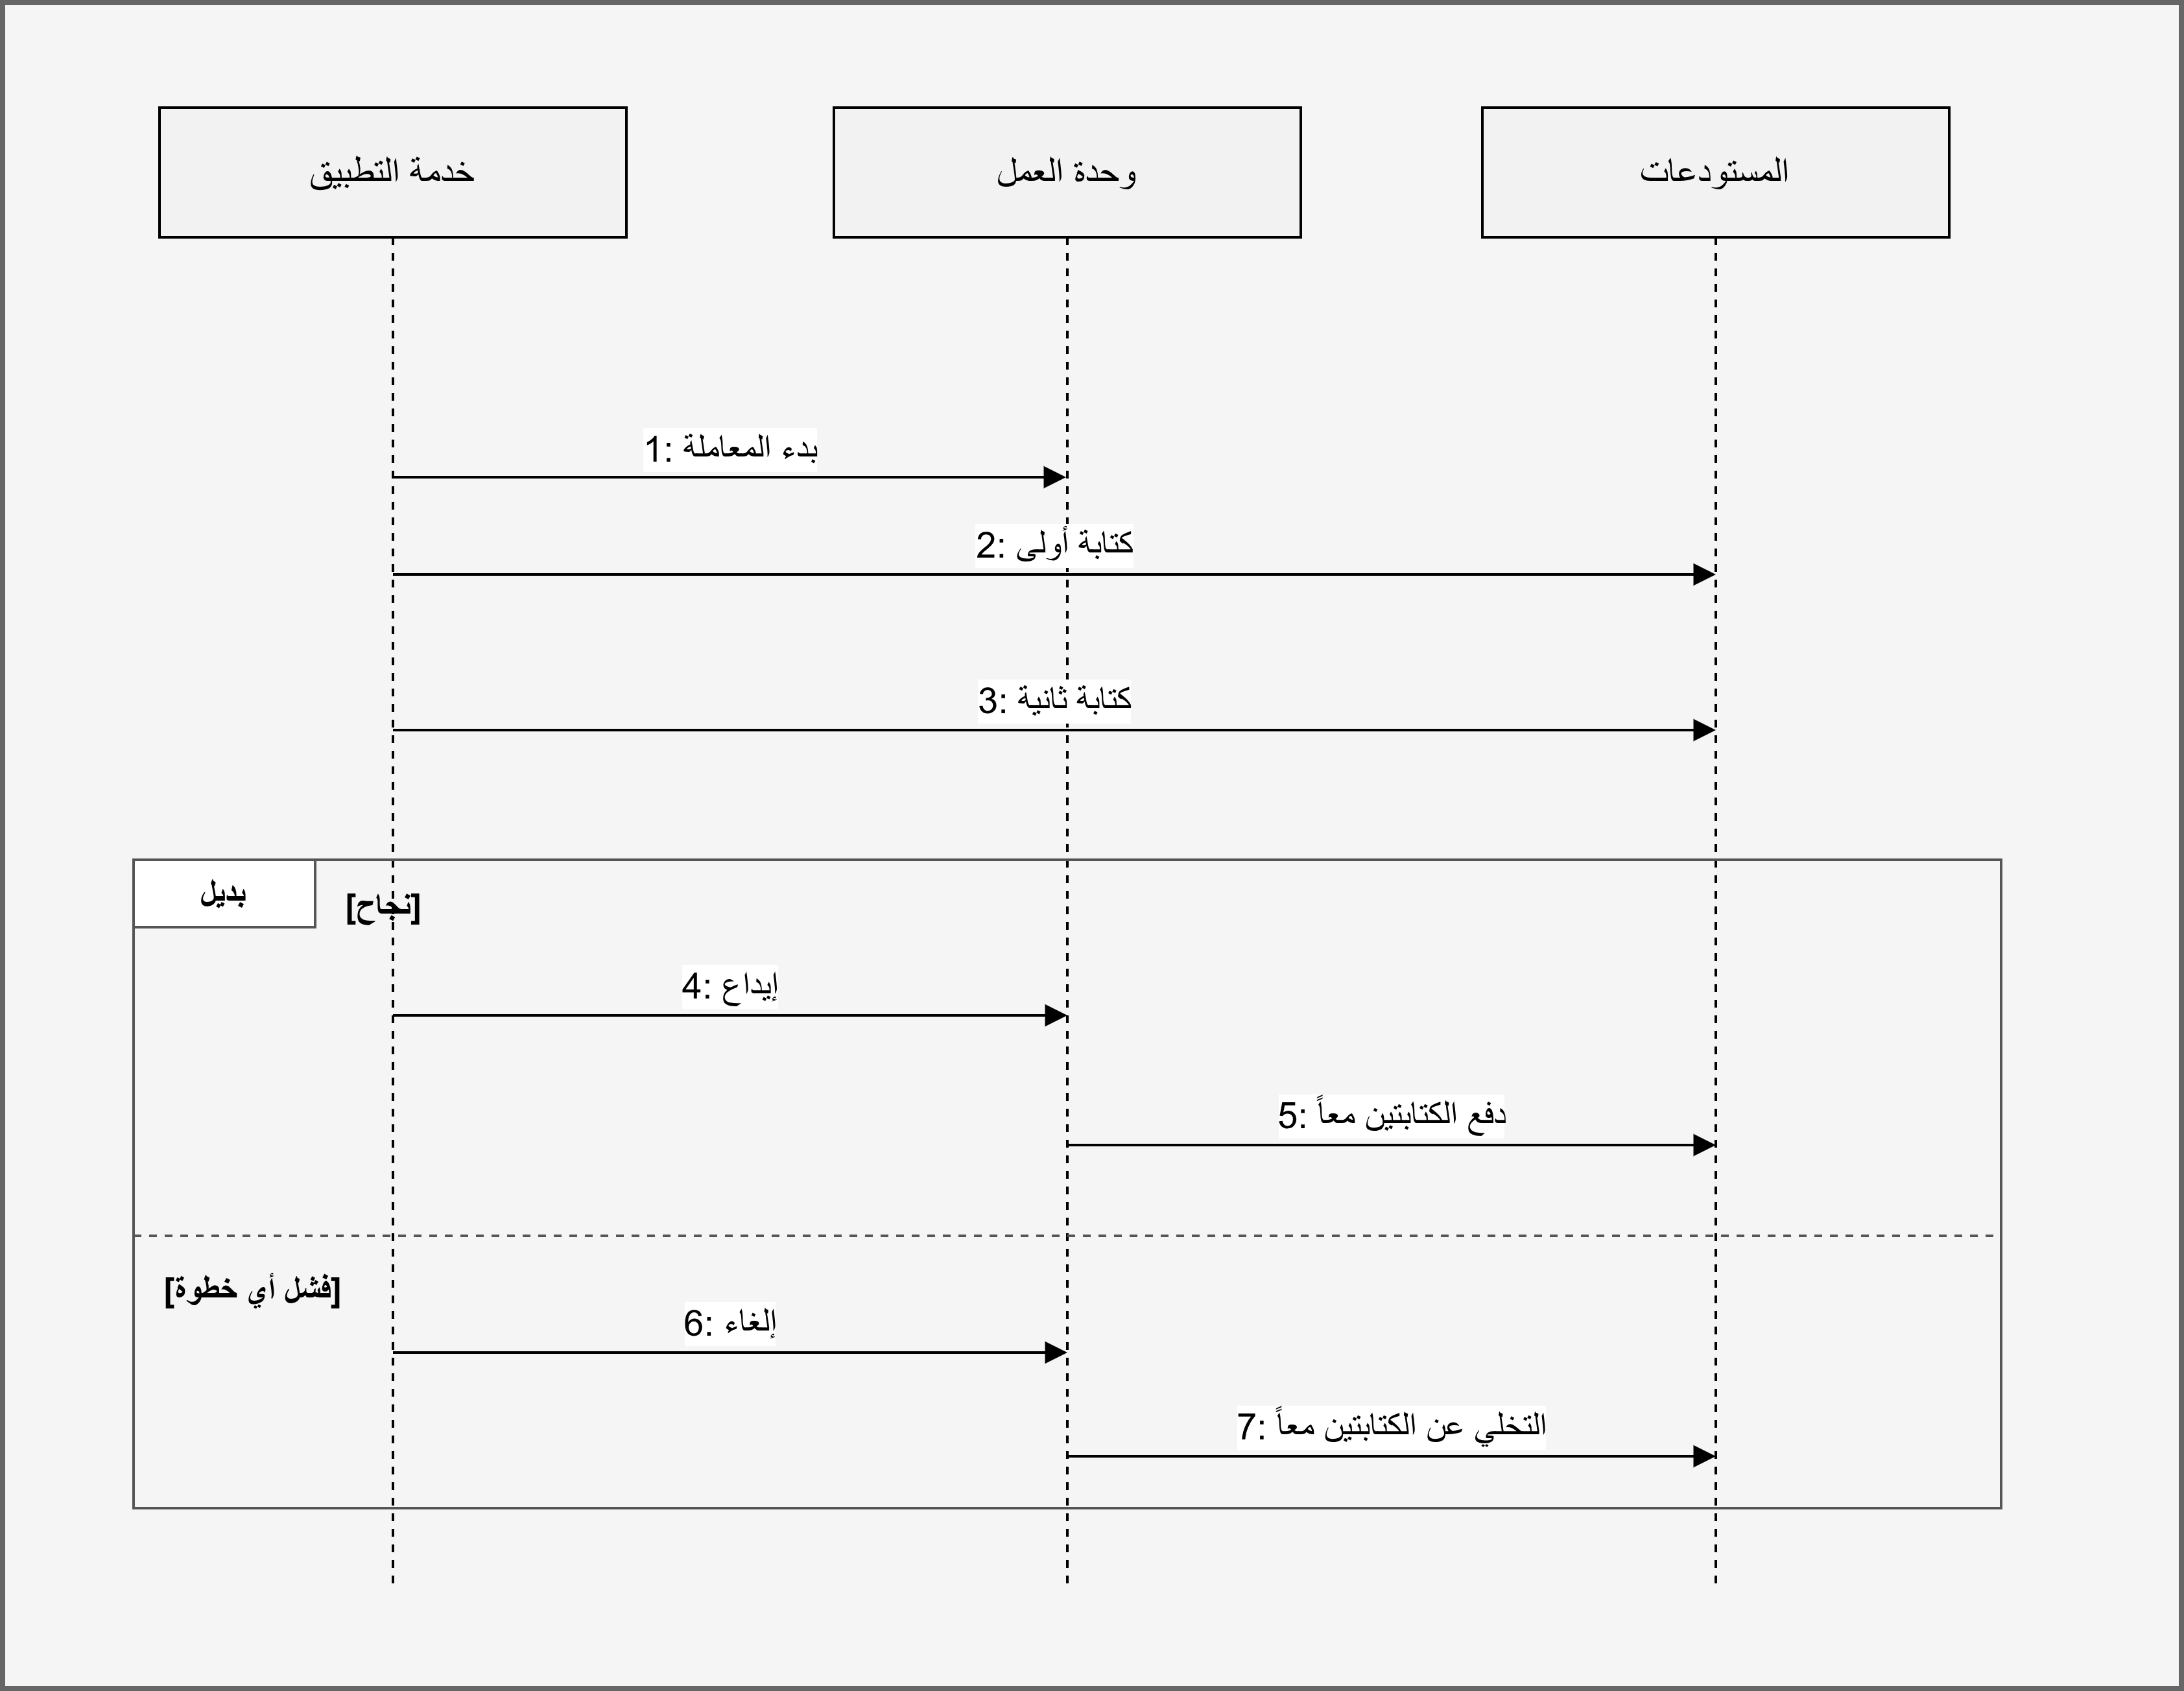
\includegraphics[width=\textwidth,height=0.8\textheight,keepaspectratio]{figures/pattern-06-unit-of-work.png}
  \caption{نمط وحدة العمل: كتابتان عبر مستودعين تحت معاملةٍ واحدة، تُودَعان معًا أو تُلغَيان معًا.}
  \label{fig:pattern-06}
\end{figure}

يعالج هذا النمط مخاطر "البيانات المتناقضة"؛ ففي عملية إنهاء الجلسة، يجب تحديث حالة الجلسة وإضافة سجل الملخص في آن واحد. لولا وحدة العمل، لكان من الممكن تحديث الجلسة وفشل إضافة سجل الملخص، مما يترك النظام في حالة غير متسقة. يوفر المنفذ \code{IUnitOfWork} العمليات اللازمة لإيداع (\en{Commit}) أو إلغاء (\en{Rollback}) المعاملة بشكل آمن.

\subsection{صندوق الصادر المعامل (\en{Transactional Outbox})}

يعد هذا النمط حلاً لمشكلة عدم إمكانية إجراء معاملة ذرية بين قاعدة البيانات وناقل الرسائل (\en{Message Bus}). يعرض الشكل~\ref{fig:pattern-07} آلية عمل هذا النمط لضمان تسليم الأحداث.

\begin{figure}[htbp]
  \centering
  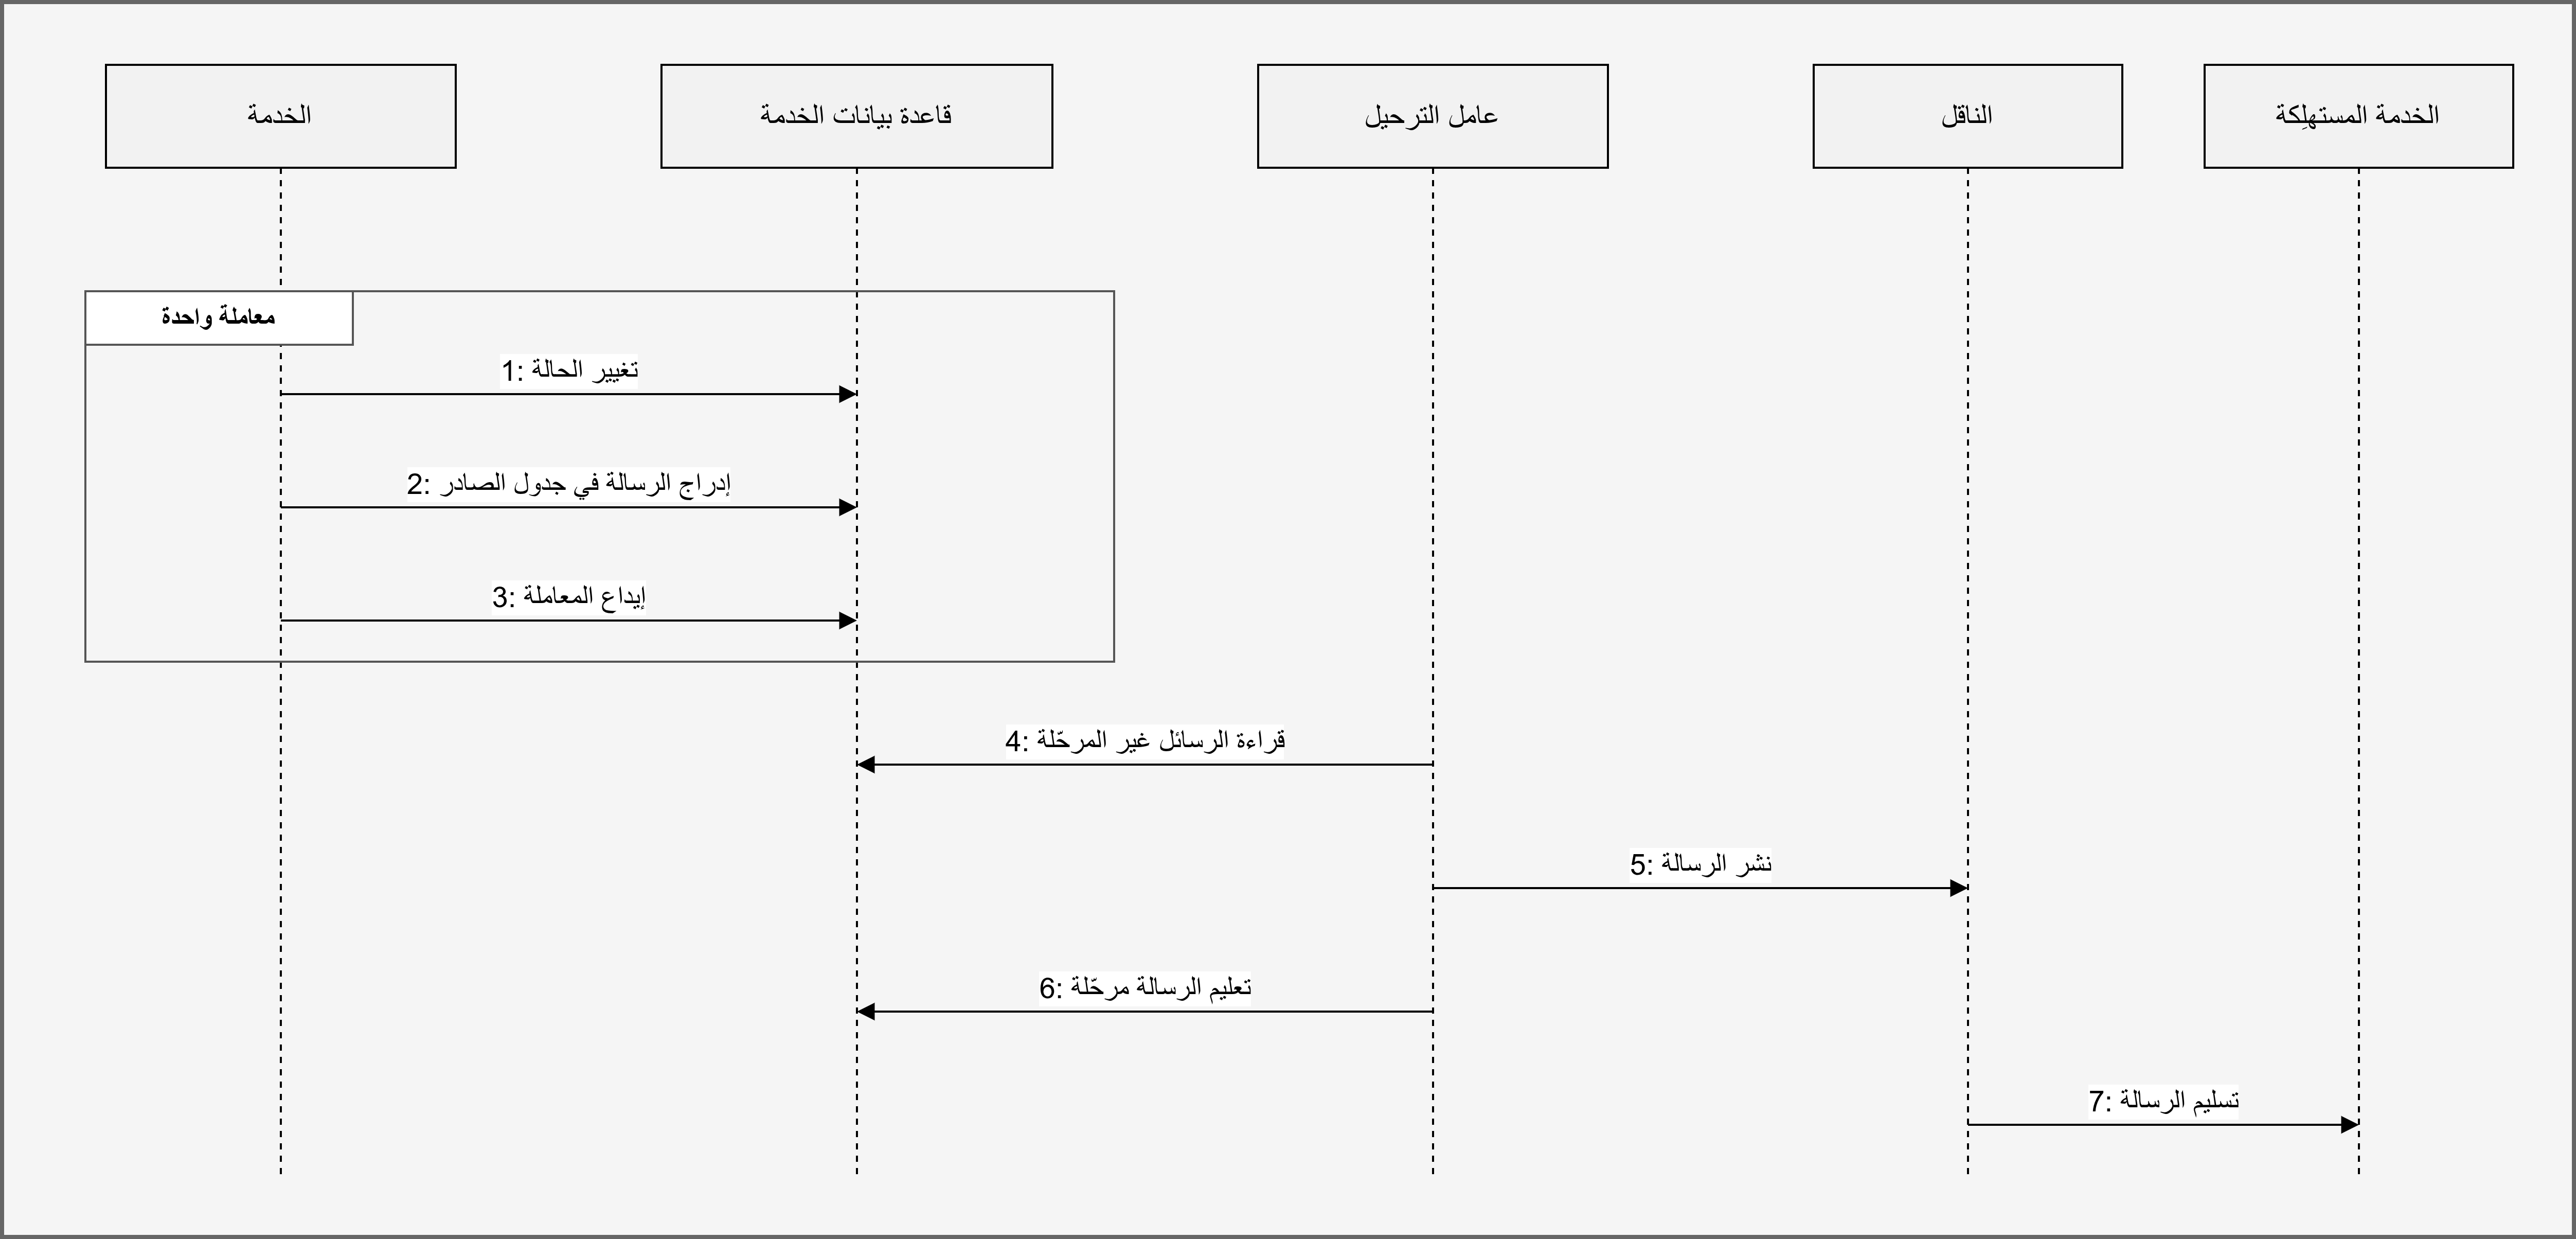
\includegraphics[width=\textwidth,height=0.8\textheight,keepaspectratio]{figures/pattern-07-transactional-outbox.png}
  \caption{نمط صندوق الصادر المعامل: تُكتَب الرسالة ضمن معاملة العمل، ثمّ يُرحّلها عامل مستقلّ.}
  \label{fig:pattern-07}
\end{figure}

عند إنهاء جلسة أو توليد ملخص، تُكتب الرسالة في جدول خاص (\code{outbox\_messages}) ضمن نفس معاملة قاعدة البيانات التي تُغير الحالة. لاحقاً، يتولى عامل ترحيل مستقل قراءة هذه الرسائل ونشرها على الناقل. يضمن هذا الإجراء وصول الإشعارات إلى الخدمات المستهلكة حتى في حال تعطل الناقل لحظياً، حيث تبقى الرسائل في الصادر حتى يتم التأكد من نشرها بنجاح.

\section{مكوّنات تطبيق الويب}
% Content for Chapter 5, Section 5.3 — pulled in by chapters/05-system-design.tex
بُني تطبيق الويب بمكتبة \en{React 19} فوق أداة البناء \en{Vite}، وقُسّم إلى شرائح وظيفية (\en{Feature Slices}) لا إلى طبقات تقنية. وتملك كل شريحة مجلّداتها الأربعة: \en{api} لنداءات الخدمات، و\en{hooks} لحالة الخادم، و\en{components} لعناصر الواجهة، و\en{types} لأنماط البيانات. ويعرض الشكل~\ref{fig:comp-07} هذه المكوّنات مع روابطها الخارجية.

\begin{figure}[htbp]
  \centering
  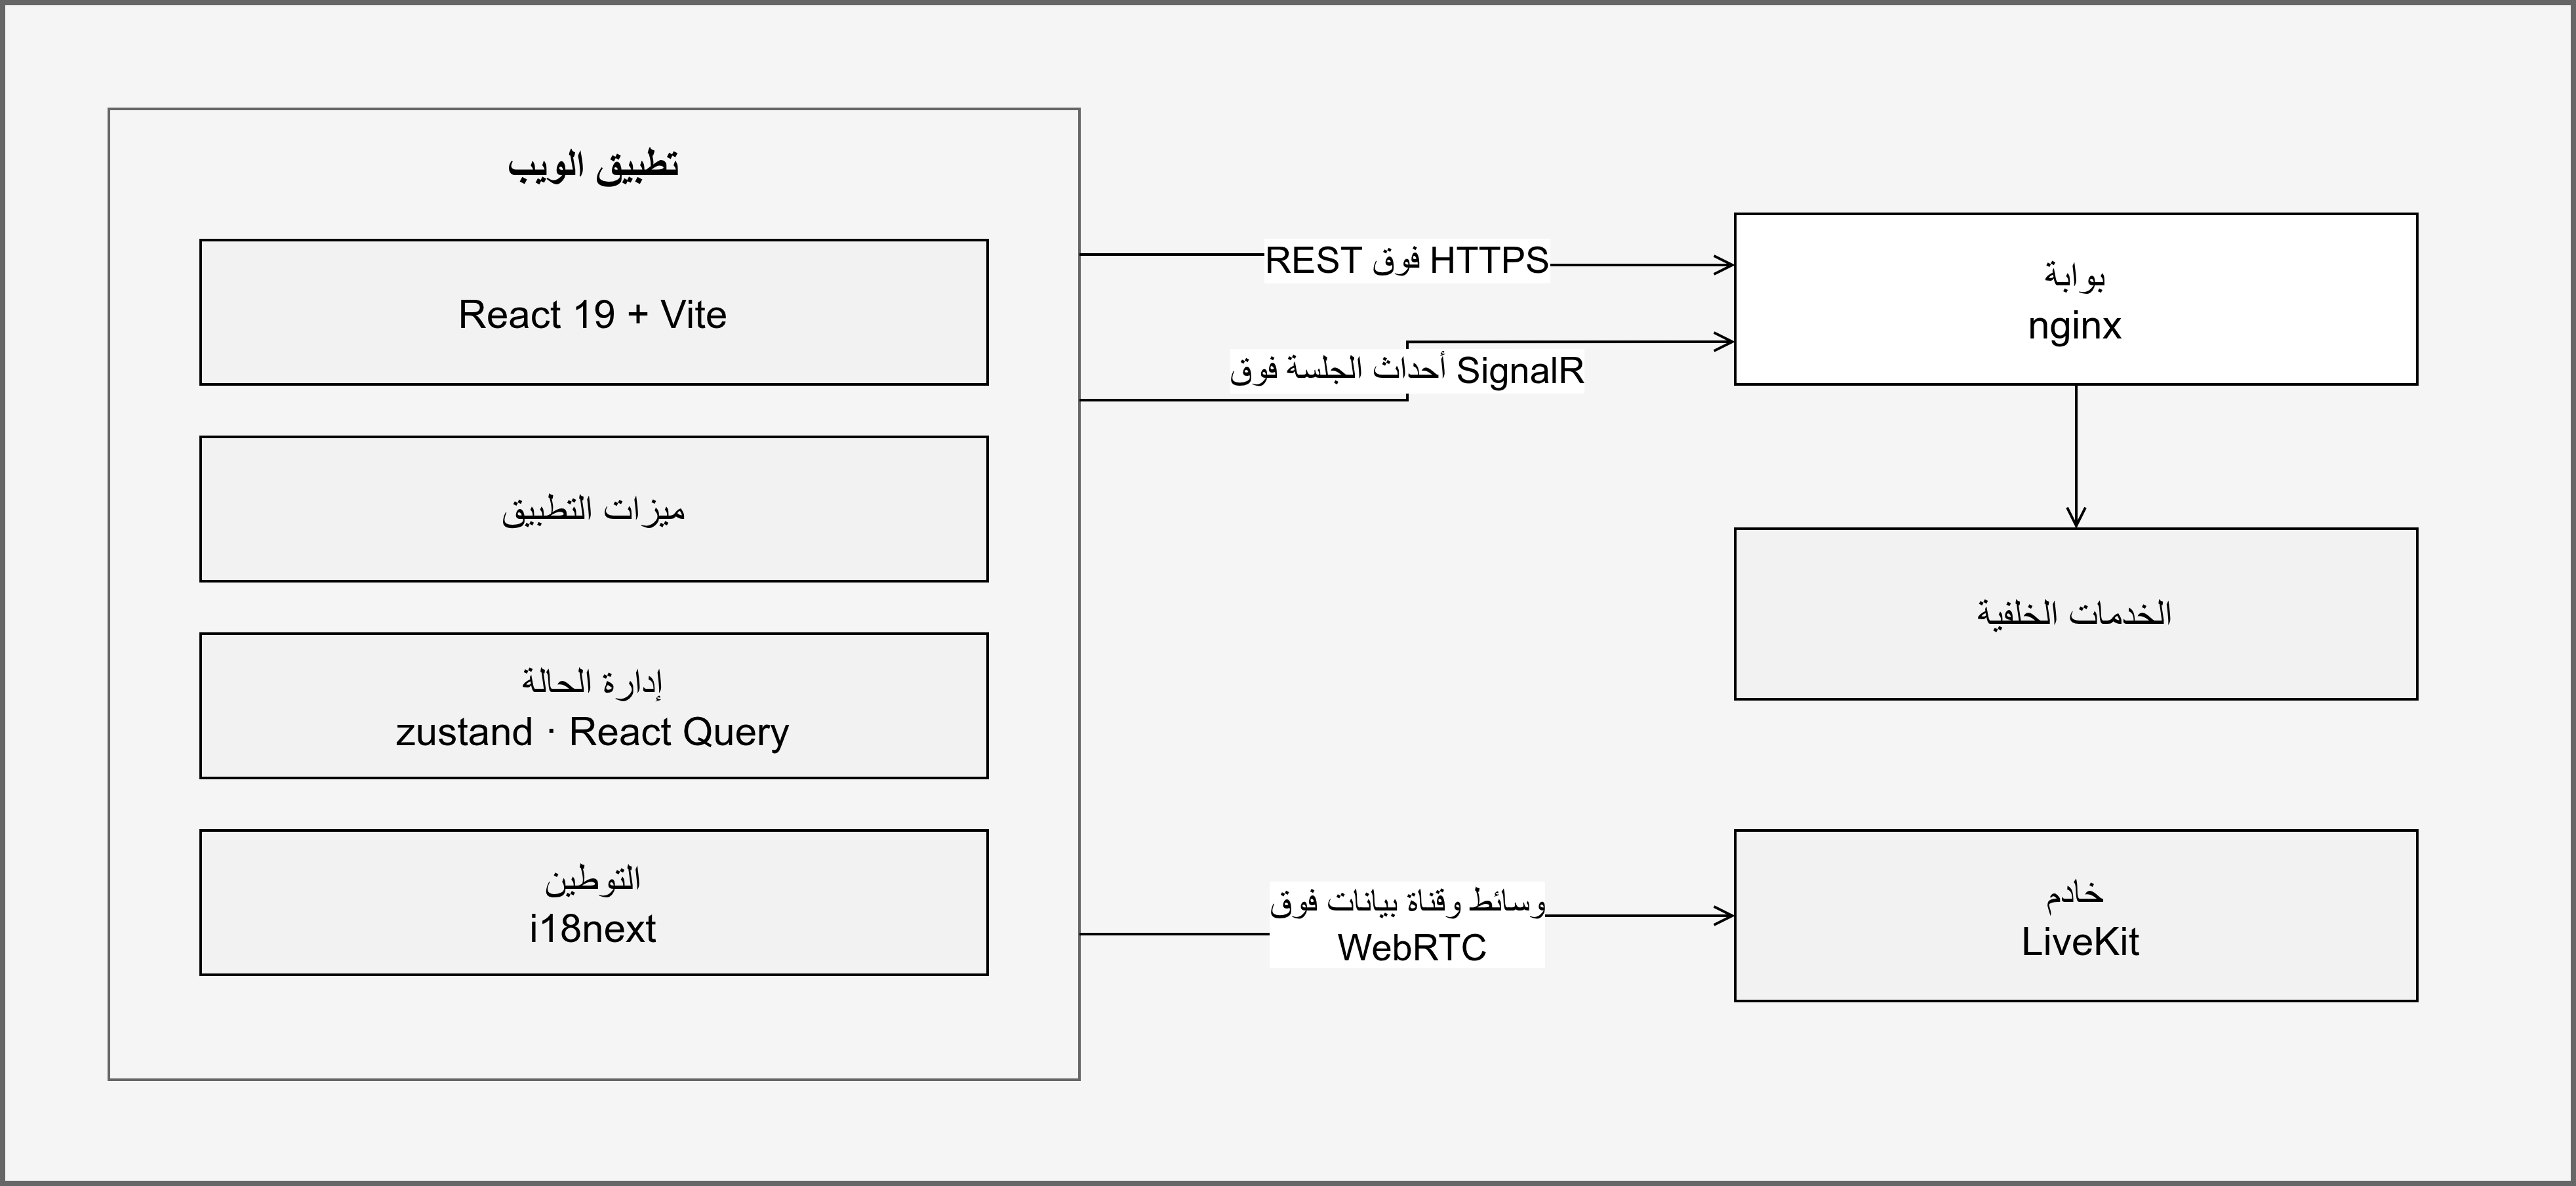
\includegraphics[width=\textwidth,height=0.8\textheight,keepaspectratio]{figures/comp-07-frontend.png}
  \caption{مخطط مكوّنات تطبيق الويب.}
  \label{fig:comp-07}
\end{figure}

ويقوم تصميم التطبيق على أربعة قرارات:

\begin{enumerate}
  \item \textbf{التقسيم بحسب الوظيفة}: تقابل الشرائح الثلاث عشرة مجالاتِ الخدمات الخلفية، فيبقى أثر أيّ تغيير محصورًا في شريحة واحدة. ويقابل التقسيم بحسب الطبقة التقنية ذلك بتوزيع الوظيفة الواحدة على مجلّدات متباعدة.
  \item \textbf{حدّ وحيد للاتصال}: تمرّ نداءات الشرائح كلّها عبر عميل \en{HTTP} واحد هو \en{apiClient}. ويُلحق هذا العميل رمز الوصول بكل طلب، ويعالج الجواب \en{401} بتجديد الرمز وإعادة إرسال الطلب مرّةً واحدة. فإن فشل التجديد محا الجلسة المحلية وأعاد التوجيه إلى صفحة الدخول، دون أن تعلم الشريحة الطالِبة بشيء من ذلك.
  \item \textbf{حراسة على مستوى المسار}: تمنع المكوّنات \en{ProtectedRoute} و\en{PublicRoute} و\en{RoleProtectedRoute} عرض المسارات غير المصرَّح بها للمستخدم الحالي. وهذه الحراسة طبقة إضافية لا حدٌّ أمني، إذ يجري التحقّق الفعلي من الصلاحية في الخدمات الخلفية عند كل طلب.
  \item \textbf{ثلاث قنوات متمايزة}: تُنقَل نداءات \en{REST} وأحداث الجلسة عبر البوّابة العكسية، الأولى فوق \en{HTTPS} والثانية فوق \en{SignalR}. أمّا الوسائط فتُنقَل عبر \en{WebRTC} مباشرةً إلى خادم \en{LiveKit} دون المرور بالبوّابة. وتجري السبّورة التشاركية على قناة بيانات \en{LiveKit} نفسها، فلا تمرّ خطوطها بالخلفية أصلًا.
\end{enumerate}

وتُدار الحالة المشتركة بمخزنَي \en{zustand}: مخزن الجلسة (\en{useAuthStore}) ومخزن السمة (\en{useThemeStore}). وتُدار حالة الخادم في خطّافات كل شريحة بوساطة \en{React Query}. ويدعم التطبيق العربية والإنكليزية عبر \en{i18next} مع تبديل اتجاه الصفحة تبعًا للّغة المختارة.


\section{خدمة إدارة المستخدمين (\en{UserManagementService})}
% Content for Chapter 5, Section 5.4 — pulled in by chapters/05-system-design.tex
\subsection{مكوّنات الخدمة}

% CH2-REF: originally "(\en{Clean Architecture}) الموصوف في القسم~\ref{subsec:clean-architecture}،" — restore with chapter 2.
اتُّبع في تصميم هذه الخدمة، كما في بقية خدمات \en{.NET}، نمطُ المعمارية النظيفة (\en{Clean Architecture})، بأربع طبقات متّحدة المركز تتّجه التبعيات فيها نحو الداخل. ويعرض الشكل~\ref{fig:comp-01} مكوّنات الخدمة موزّعةً على هذه الطبقات مع روابطها الخارجية.

\begin{figure}[htbp]
  \centering
  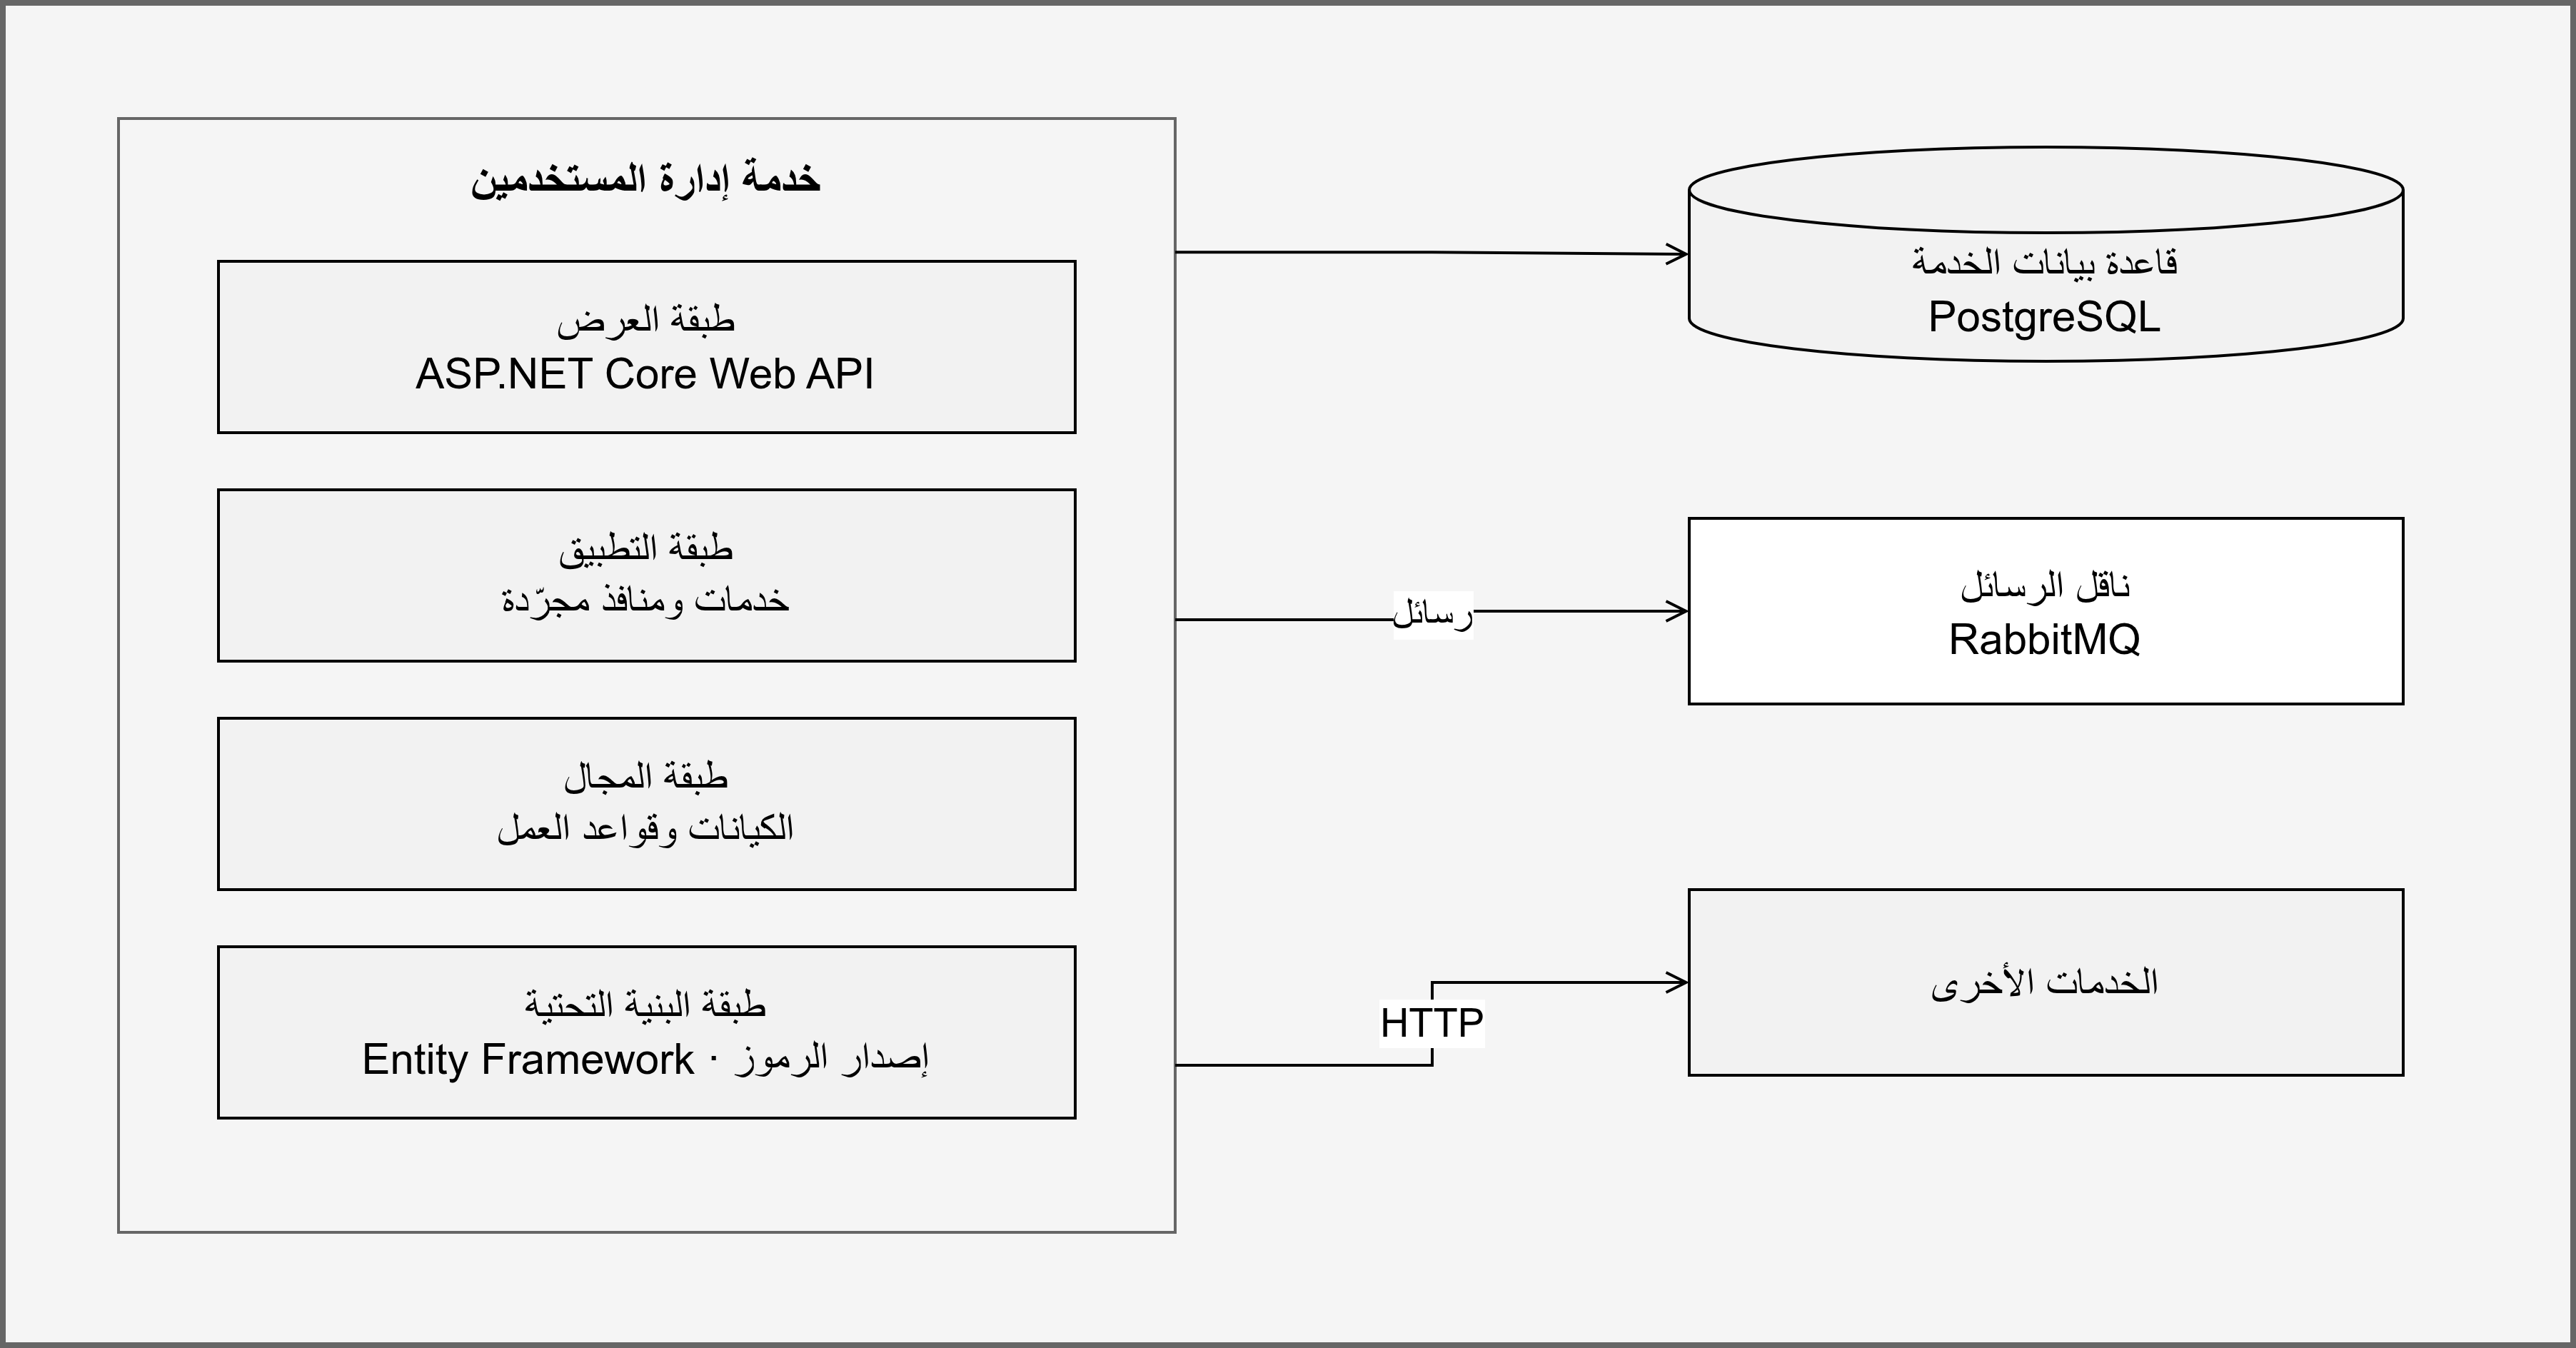
\includegraphics[width=\textwidth,height=0.8\textheight,keepaspectratio]{figures/comp-01-user-management.png}
  \caption{مخطط المكوّنات التفصيلي لخدمة إدارة المستخدمين.}
  \label{fig:comp-01}
\end{figure}

وتتّصل الخدمة بمحيطها عبر ثلاثة مسارات:

\begin{enumerate}
  \item \textbf{مولّد الرموز} (\en{JwtTokenGenerator}): تنفرد هذه الخدمة بإصدار رموز الوصول، بينما تكتفي بقية الخدمات بالتحقّق منها. ويحصر هذا التمركز أيّ تعديل على سياسة المصادقة في موضع واحد.
  \item \textbf{ناقل الإشعارات} (\en{INotificationBus}): يُستعمل لنشر ما يتطلّب تنفيذ إجراء في خدمة أخرى، كإرسال رمز العامل الثاني أو الإعلام بتغيّر حالة مستخدم.
  \item \textbf{عملاء \en{HTTP} الداخليون}: تستعملهم الواجهات الإدارية العابرة للخدمات، إذ يحتاج المدير الأعلى إلى الاطّلاع على الفصول والجلسات والمخرجات المملوكة لخدمات أخرى والتصرّف بها.
\end{enumerate}

ويُستعمل ناقل الإشعارات هنا بصيغته المباشرة، دون صندوق الصادر المعتمد في خدمة الفصول. ويقتضي نمط صندوق الصادر أن تجري الكتابة المقابلة في القاعدة نفسها وضمن المعاملة نفسها، وهو شرط لا يتحقّق حين يكون أثر الرسالة في قاعدة خدمة أخرى.

\subsection{نموذج البيانات}

يقوم نموذج بيانات الخدمة على خمسة كيانات يعرضها الشكل~\ref{fig:erd-01}: المستخدم (\en{users}) والدور (\en{roles})، ورموز التحديث (\en{refresh\_tokens})، ورموز استعادة كلمة المرور (\en{reset\_password\_tokens})، وتحدّيات العامل الثاني (\en{two\_factor\_challenges}).

\begin{figure}[htbp]
  \centering
  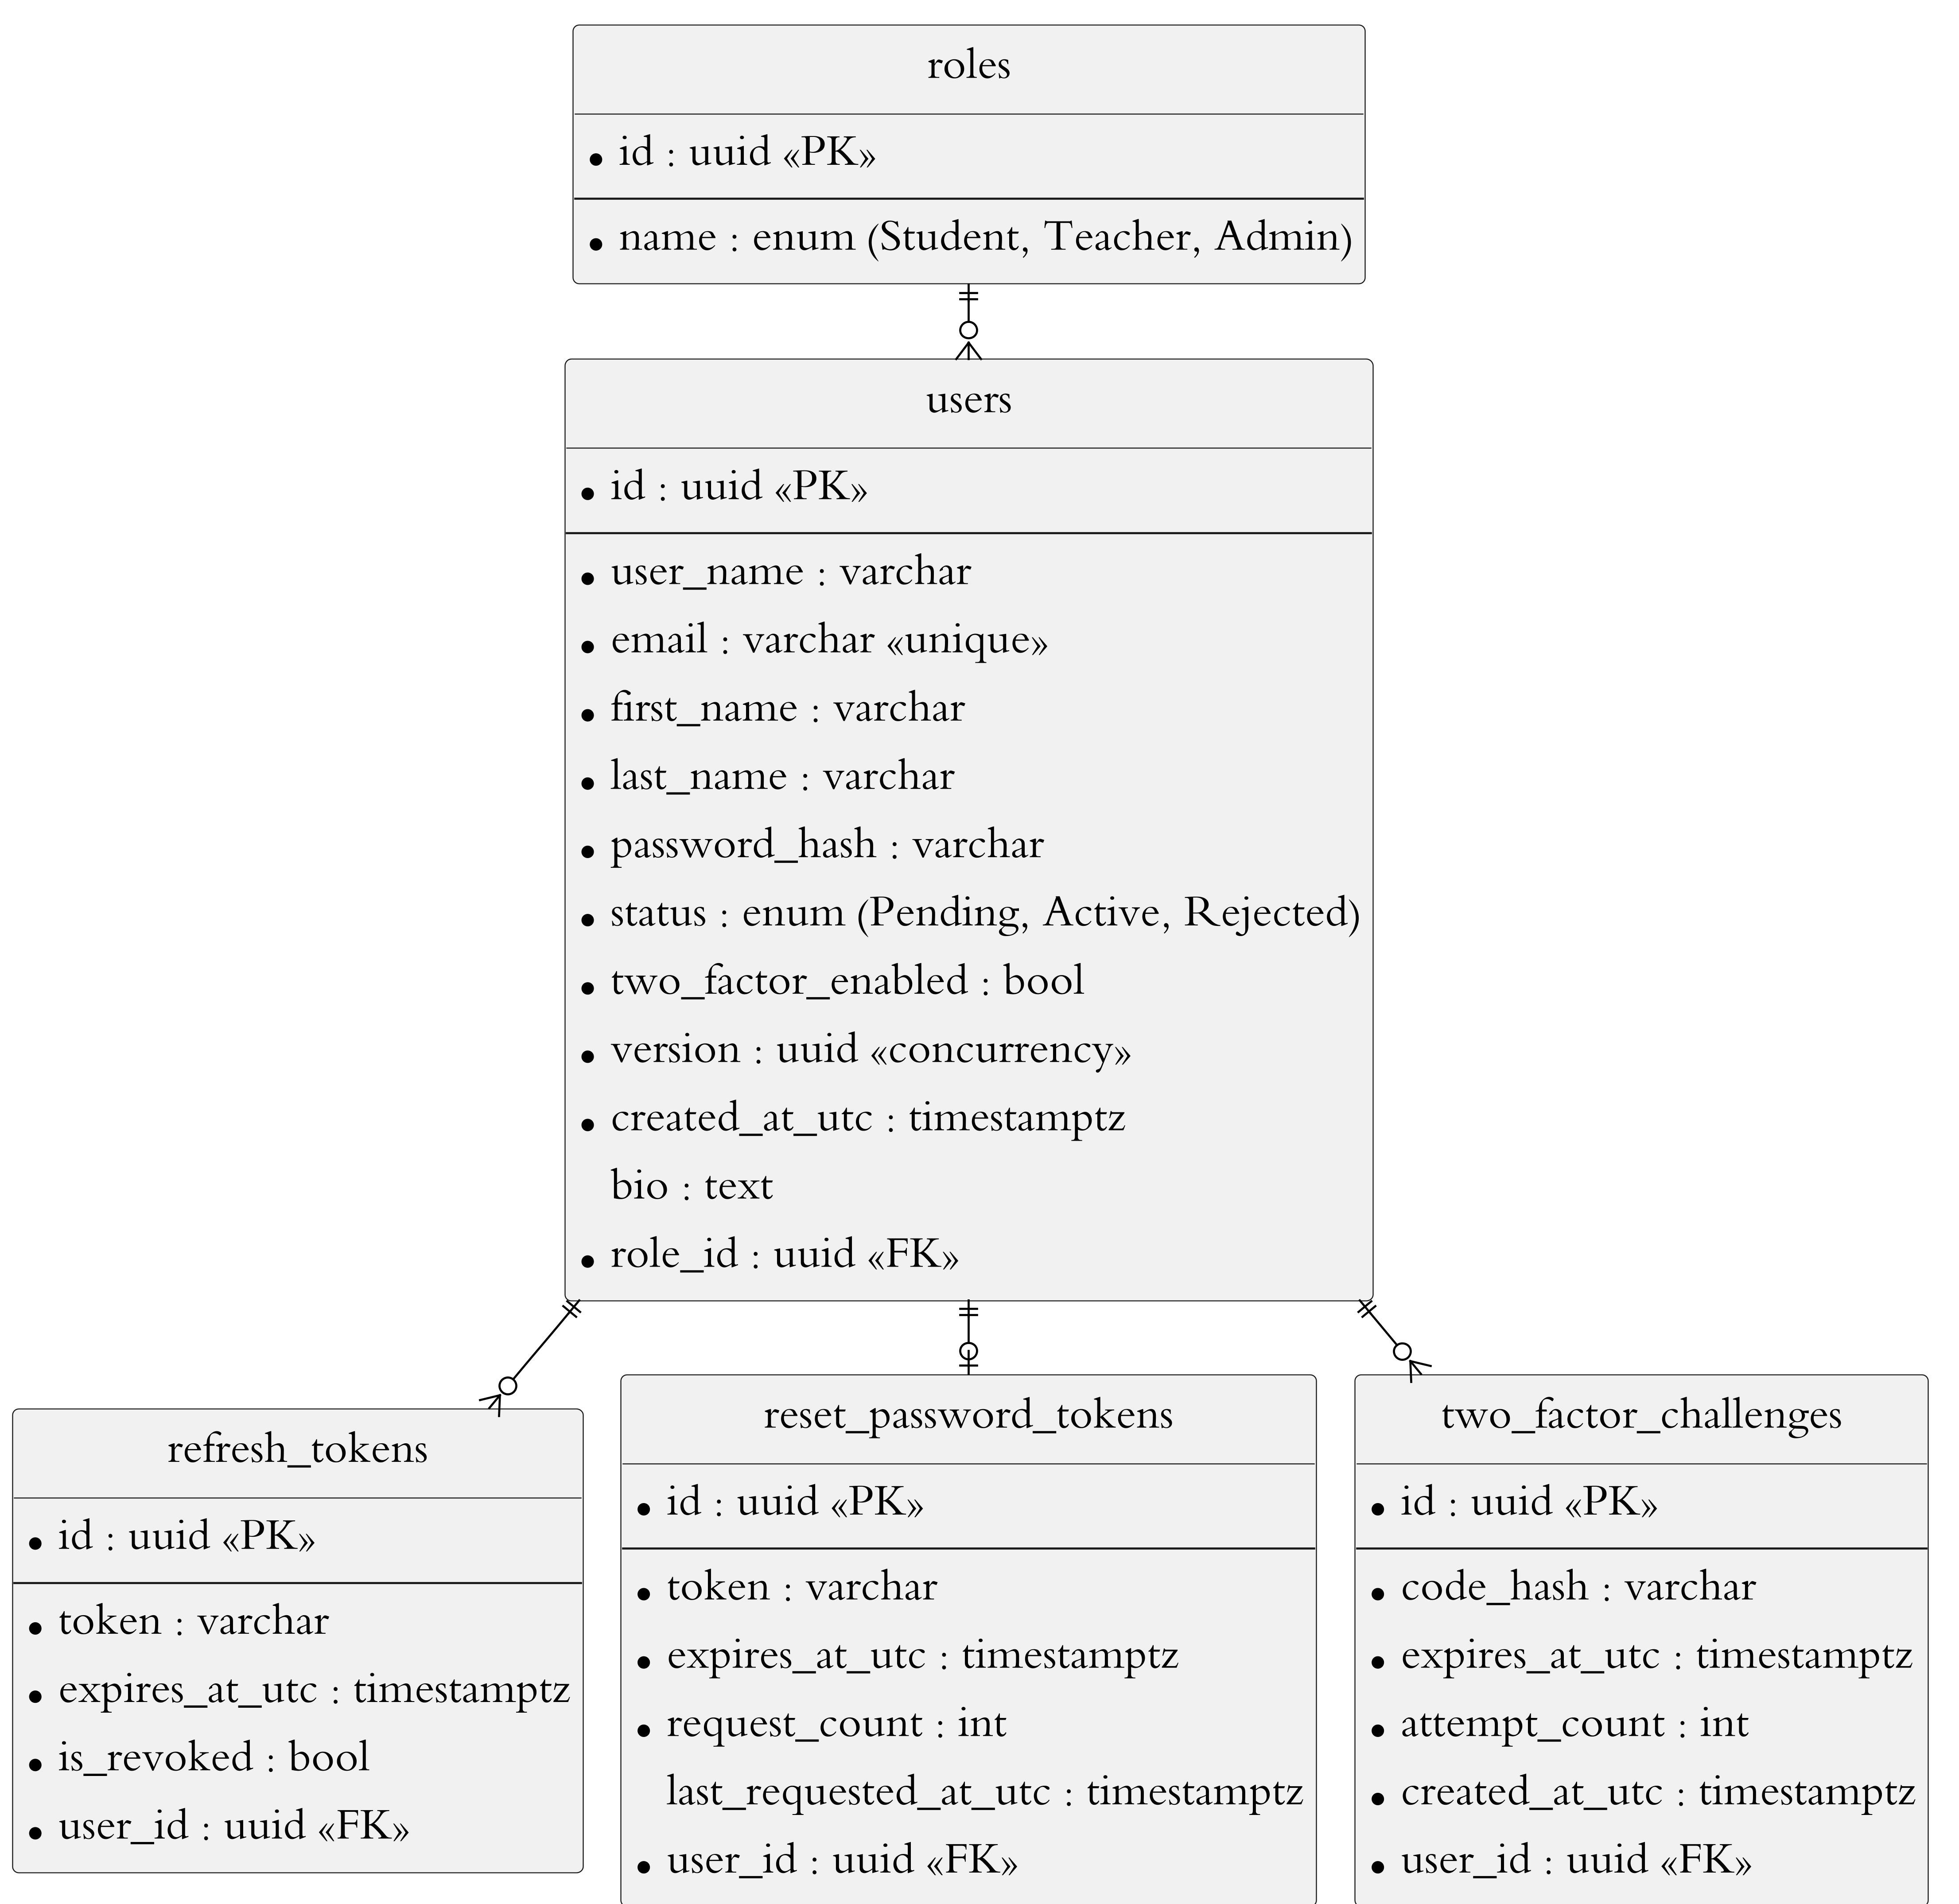
\includegraphics[width=\textwidth,height=0.8\textheight,keepaspectratio]{figures/erd-01-user-management.png}
  \caption{مخطط الكيانات والعلاقات لخدمة إدارة المستخدمين.}
  \label{fig:erd-01}
\end{figure}

وتُخزَّن الرموز الحسّاسة، وهي رمز الاستعادة ورمز العامل الثاني، على هيئة بصمات لا نصوص صريحة. ولا يمنح تسريب قاعدة البيانات عندئذٍ رمزًا صالحًا للاستعمال.

ويُبيَّن تدفّق تسجيل دخول المدير الأعلى بمرحلتيه، وما يقوم عليه من ضوابط أمنية، في القسم~\ref{subsubsec:flow-super-admin-login}.


\section{خدمة الفصول الدراسية (\en{ClassroomService})}
% Content for Chapter 5, Section 5.5 — pulled in by chapters/05-system-design.tex
\subsection{مكوّنات الخدمة}

تضمّ هذه الخدمة ثماني عشرة خدمة تطبيقية، وهي أكبر خدمات النظام حجمًا. ويعرضها الشكل~\ref{fig:comp-02} مجمّعةً بحسب المسؤولية التي تملكها كل مجموعة.

\begin{figure}[htbp]
  \centering
  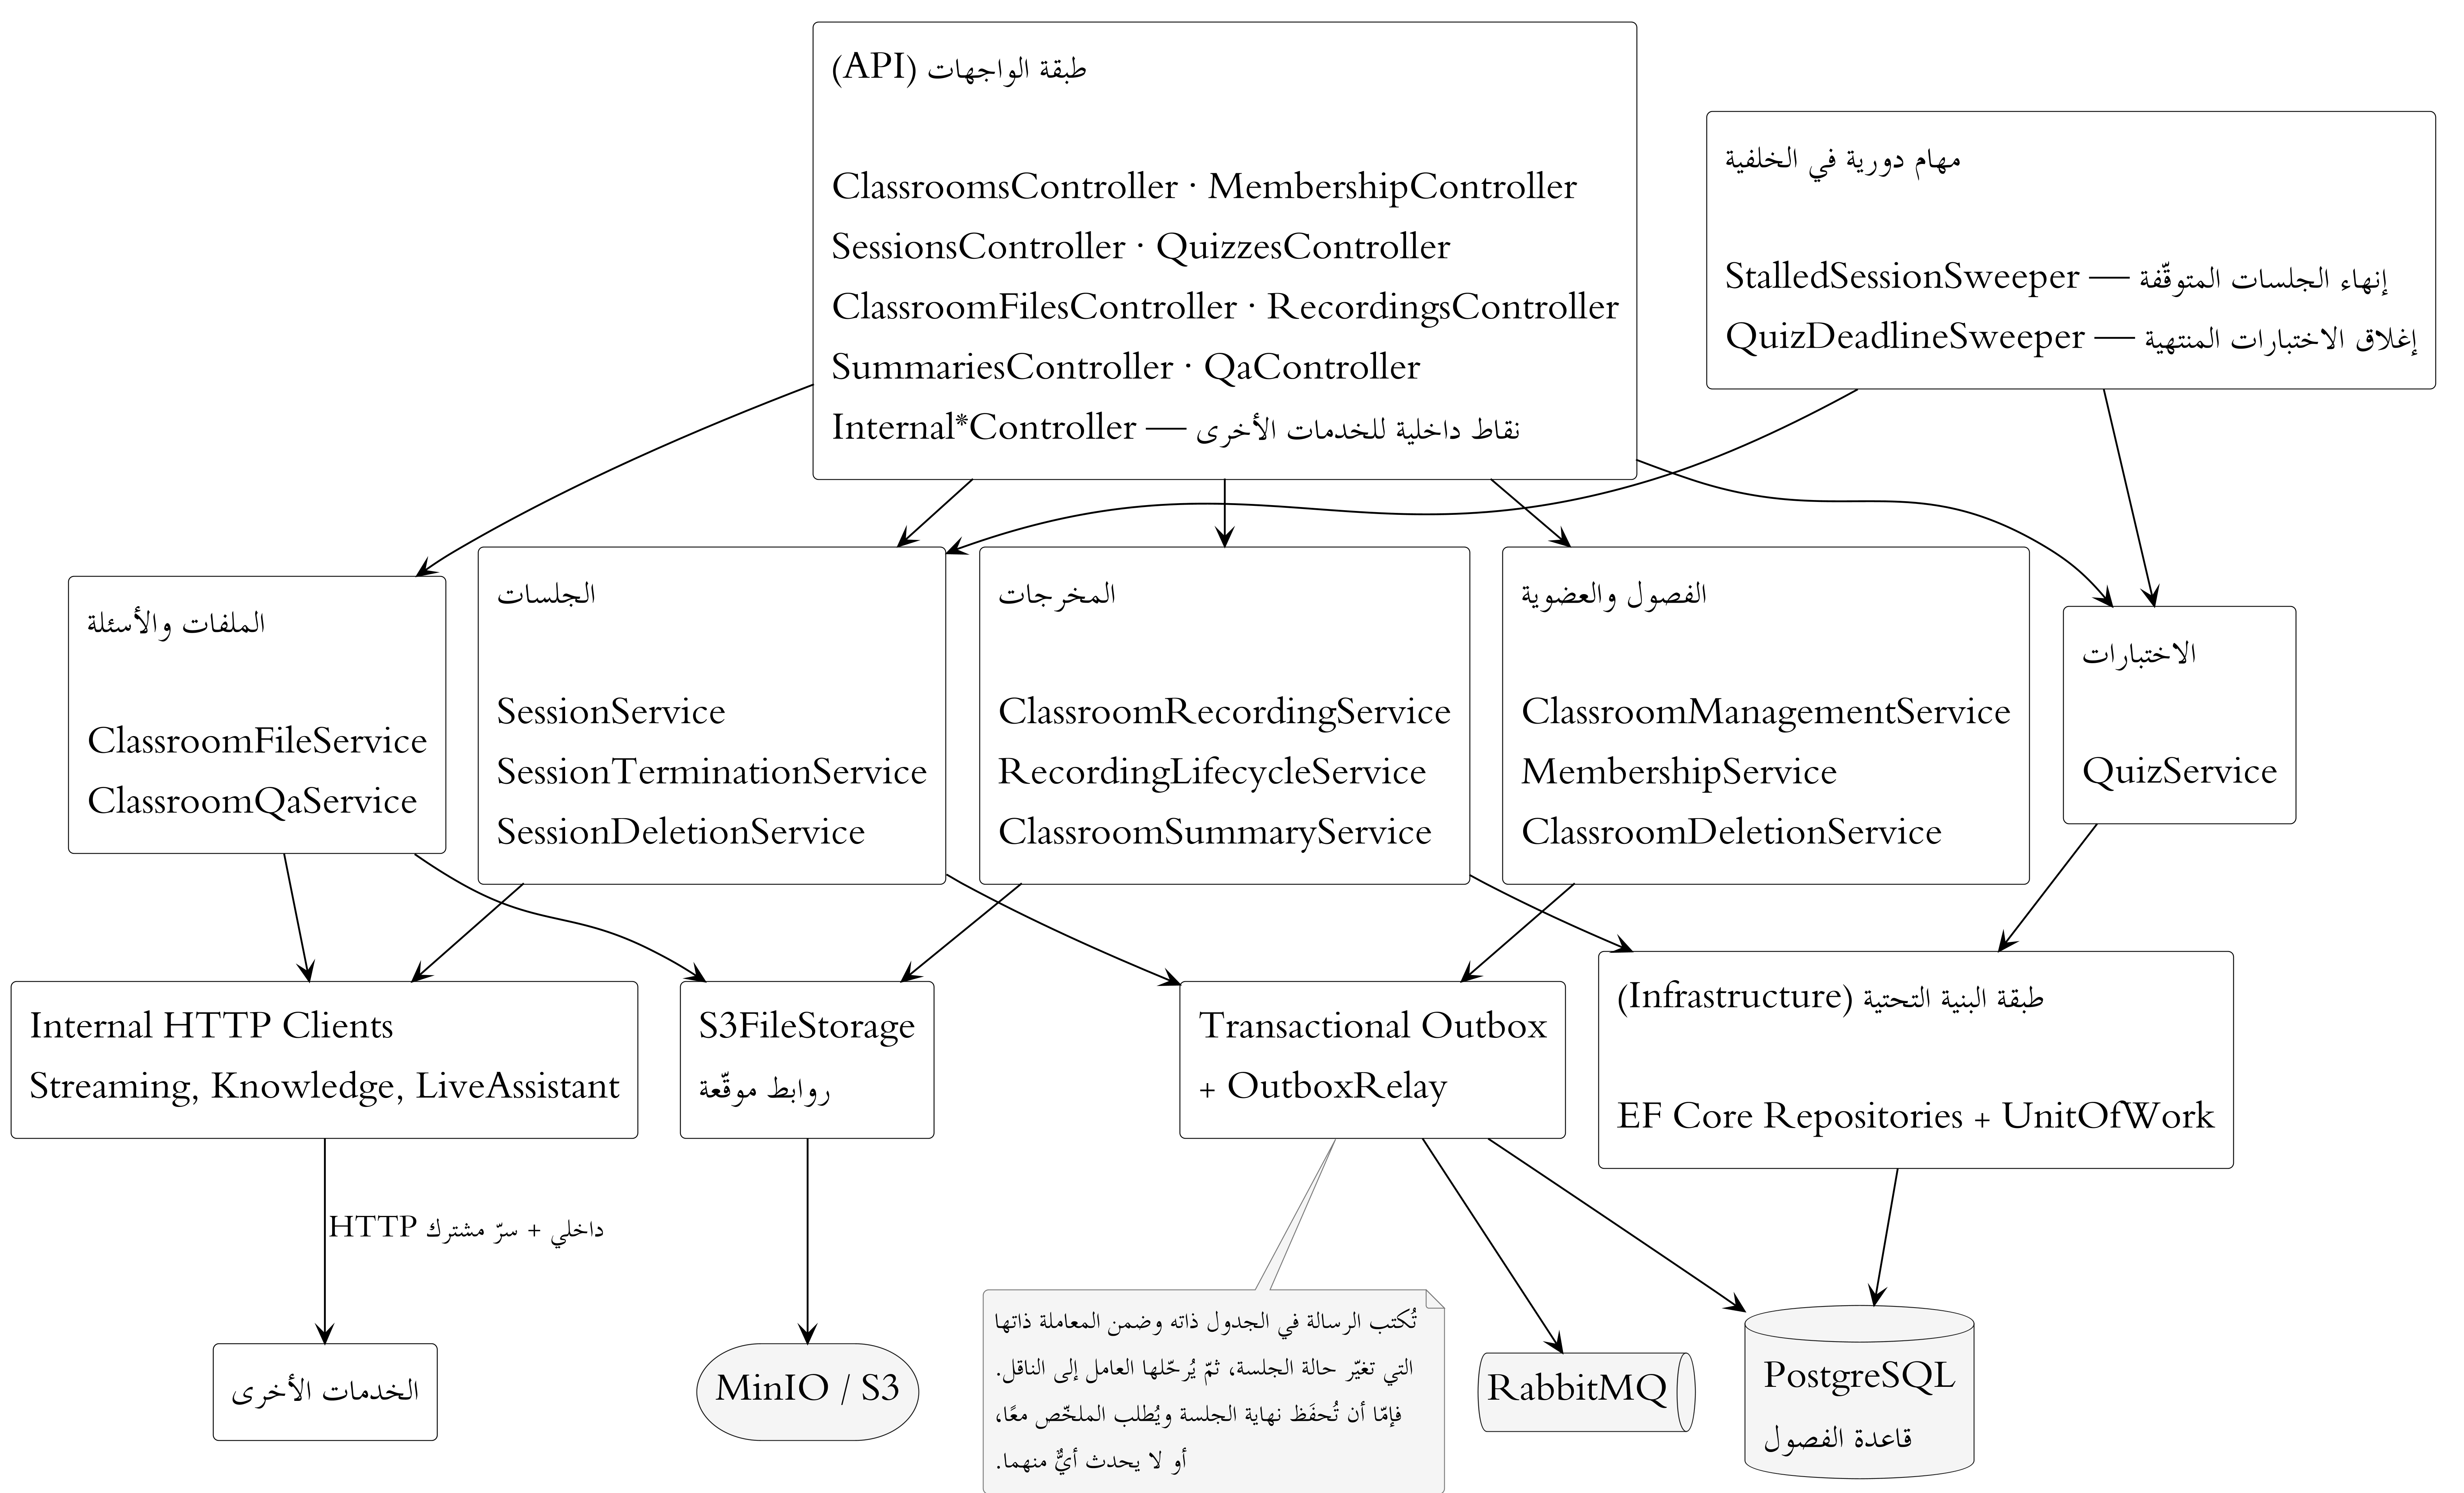
\includegraphics[width=\textwidth,height=0.8\textheight,keepaspectratio]{figures/comp-02-classroom.png}
  \caption{مخطط المكوّنات التفصيلي لخدمة الفصول الدراسية.}
  \label{fig:comp-02}
\end{figure}

وتظهر المهام الدورية في الخلفية منفصلةً عن بقية المكوّنات، لأنّها لا تُستدعى من أيّ مكوّن آخر بل تعمل على مؤقّتات. وتتولّى هذه المهام تصحيح الحالات الشاذّة، كانقطاع اتصال المعلّم في أثناء الجلسة أو انقضاء موعد إغلاق اختبار.

وترتبط هذه الخدمة بمحيطها عبر ثلاثة مسارات:

\begin{enumerate}
  \item \textbf{صندوق الصادر}: تنشر عبره أحداث المجال إلى الناقل.
  \item \textbf{مخزن الملفّات}: تحفظ فيه المواد المرجعية ومخرجات الجلسات، وتُصدر منه روابط موقَّعة محدودة المدّة.
  \item \textbf{عملاء \en{HTTP} الداخليون}: تُشغّل بهم الفهرسة في خدمة المعرفة، وتفكيك الغرف في خدمة البث، وتوليد الاختبارات في خدمة المساعد الحيّ.
\end{enumerate}

\subsection{نموذج البيانات}

يضمّ نموذج بيانات الخدمة اثني عشر كيانًا يعرضها الشكل~\ref{fig:erd-02}، موزّعةً على أربع مجموعات: الفصول وملفّاتها وعضويّاتها، والجلسات، ومخرجات الجلسات من تسجيلات وملخّصات، والاختبارات وهي المجموعة الأكبر.

\begin{figure}[htbp]
  \centering
  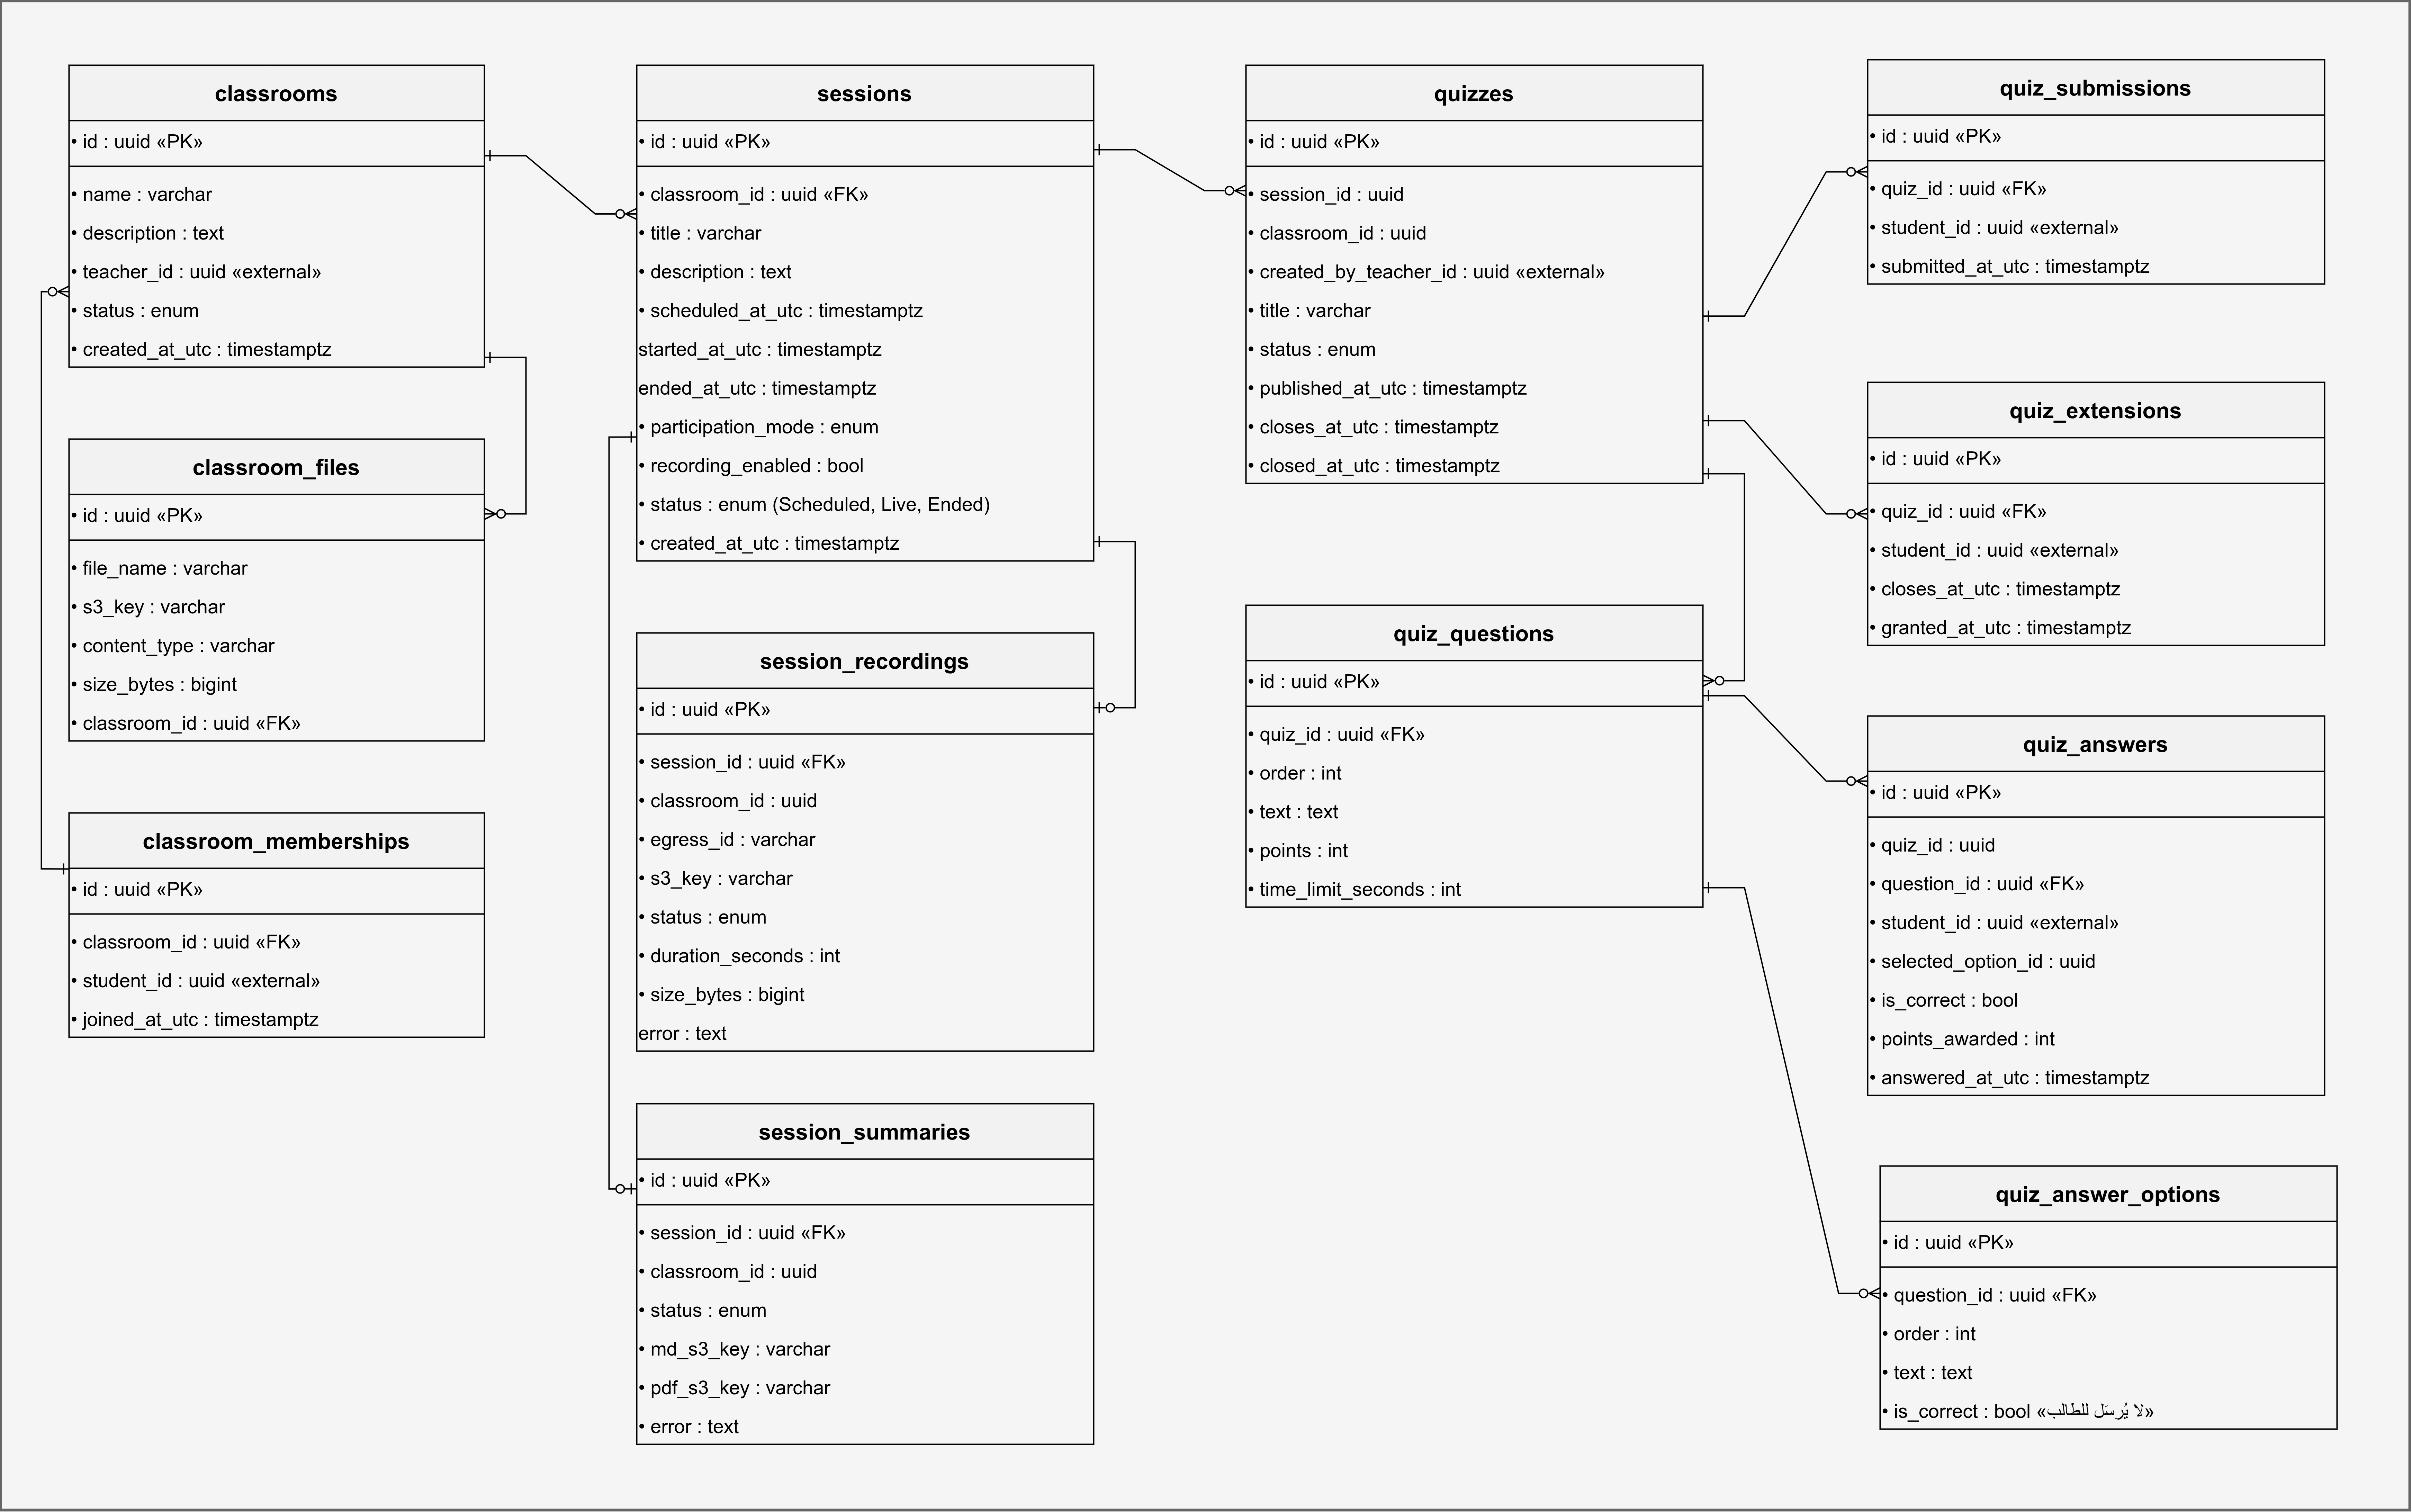
\includegraphics[width=\textwidth,height=0.8\textheight,keepaspectratio]{figures/erd-02-classroom.png}
  \caption{مخطط الكيانات والعلاقات لخدمة الفصول الدراسية.}
  \label{fig:erd-02}
\end{figure}

ويعرض الشكل~\ref{fig:class-02} تصميم تجميعة الاختبار (\en{Quiz Aggregate}) بمزيد من التفصيل.

\begin{figure}[htbp]
  \centering
  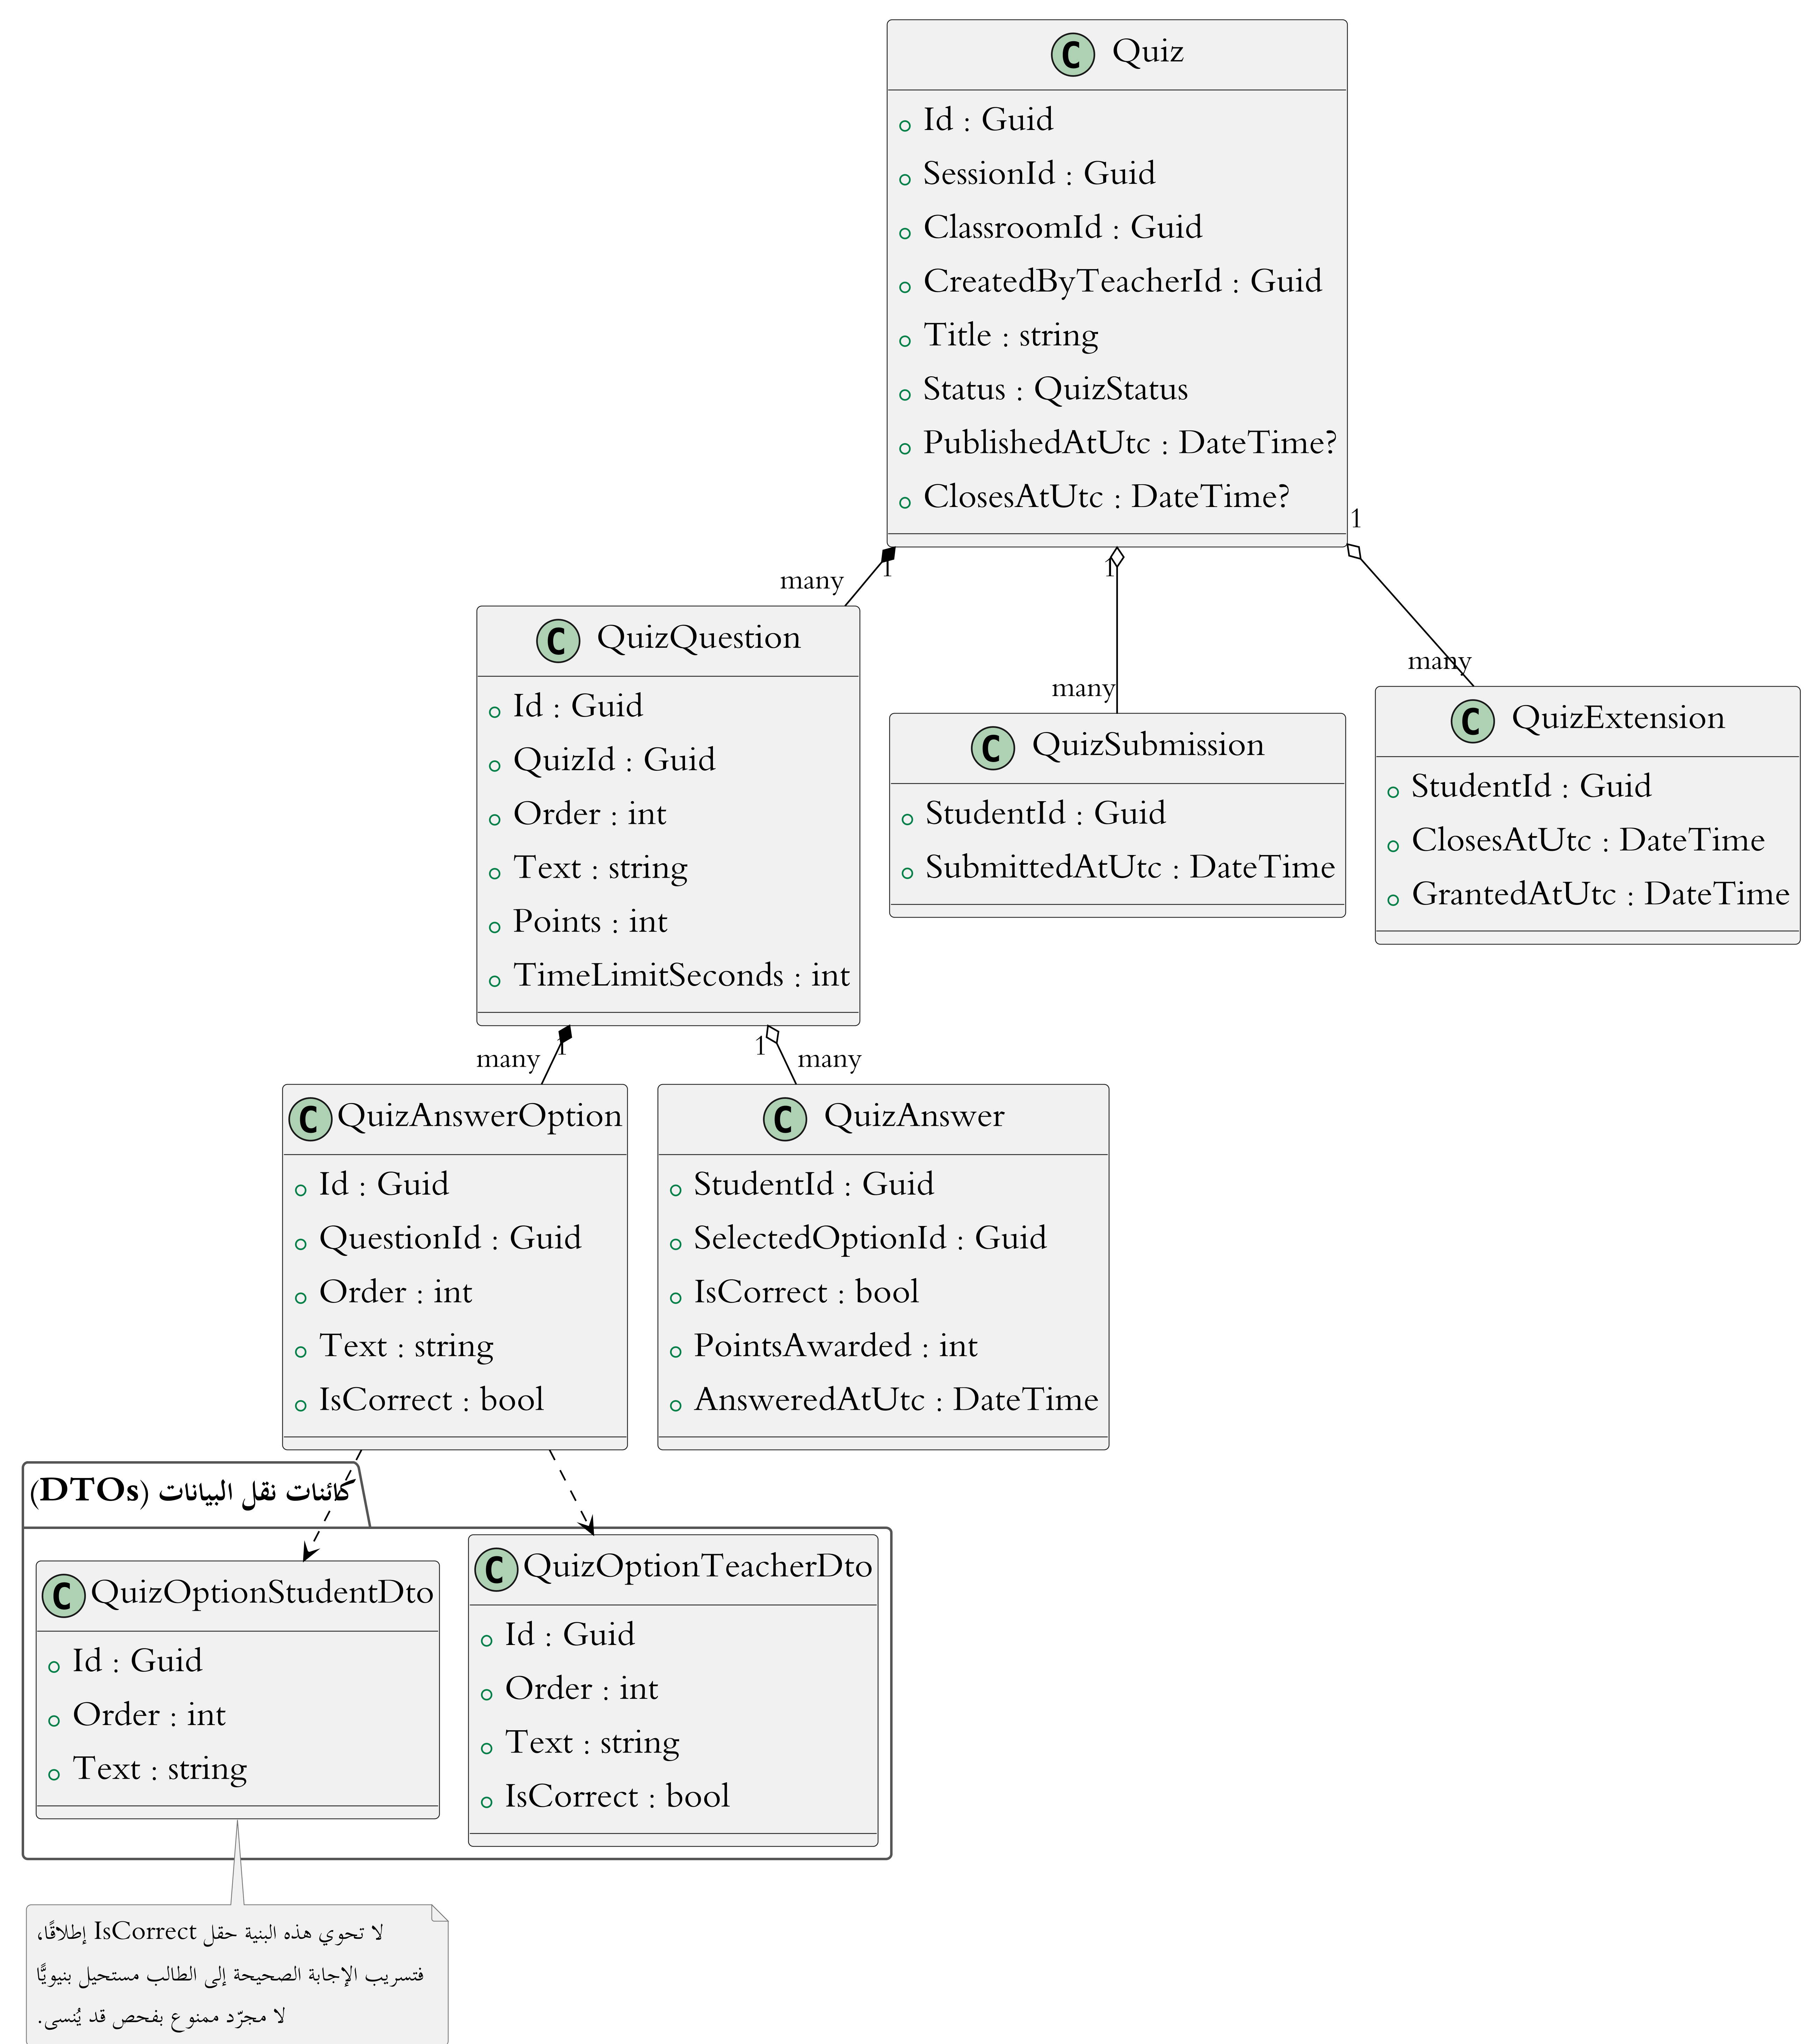
\includegraphics[width=\textwidth,height=0.8\textheight,keepaspectratio]{figures/class-02-quiz-domain.png}
  \caption{مخطط الصفوف لتجميعة الاختبار في خدمة الفصول الدراسية.}
  \label{fig:class-02}
\end{figure}

ويُحفظ الخيار الصحيح لكل سؤال في الحقل \en{IsCorrect} ضمن الكيان \en{QuizAnswerOption}. ولمنع وصول هذا الحقل إلى الطالب، عُرّفت بنيتان منفصلتان لنقل البيانات: بنية للمعلّم تتضمّن الحقل، وبنية للطالب لا تتضمّنه. ويمنع هذا الفصل البنيوي تسريب الإجابة الصحيحة، خلافًا للفحص البرمجي الذي قد يُغفَل عند إضافة مسار جديد.

ويُبيَّن تدفّق إنهاء الجلسة الحيّة، وما يعالجه من مشكلات السباق والذرّية والترتيب، في القسم~\ref{subsubsec:flow-session-end}.


\section{خدمة البث (\en{StreamingService})}
% Content for Chapter 5, Section 5.6 — pulled in by chapters/05-system-design.tex
\subsection{مكوّنات الخدمة}

تضمّ طبقة التطبيق في هذه الخدمة خدمة واحدة، ويقع معظم التعقيد في طبقة البنية التحتية، لأن التسجيل عملية يقودها نظام خارجي يُجيب لاحقاً بإشعار غير مضمون الوصول. ويعرض الشكل~\ref{fig:comp-03} مكوّنات الخدمة وروابطها الخارجية.

\begin{figure}[htbp]
  \centering
  % 2.20:1 — full width is ~30% of the text block, so it places inline.
  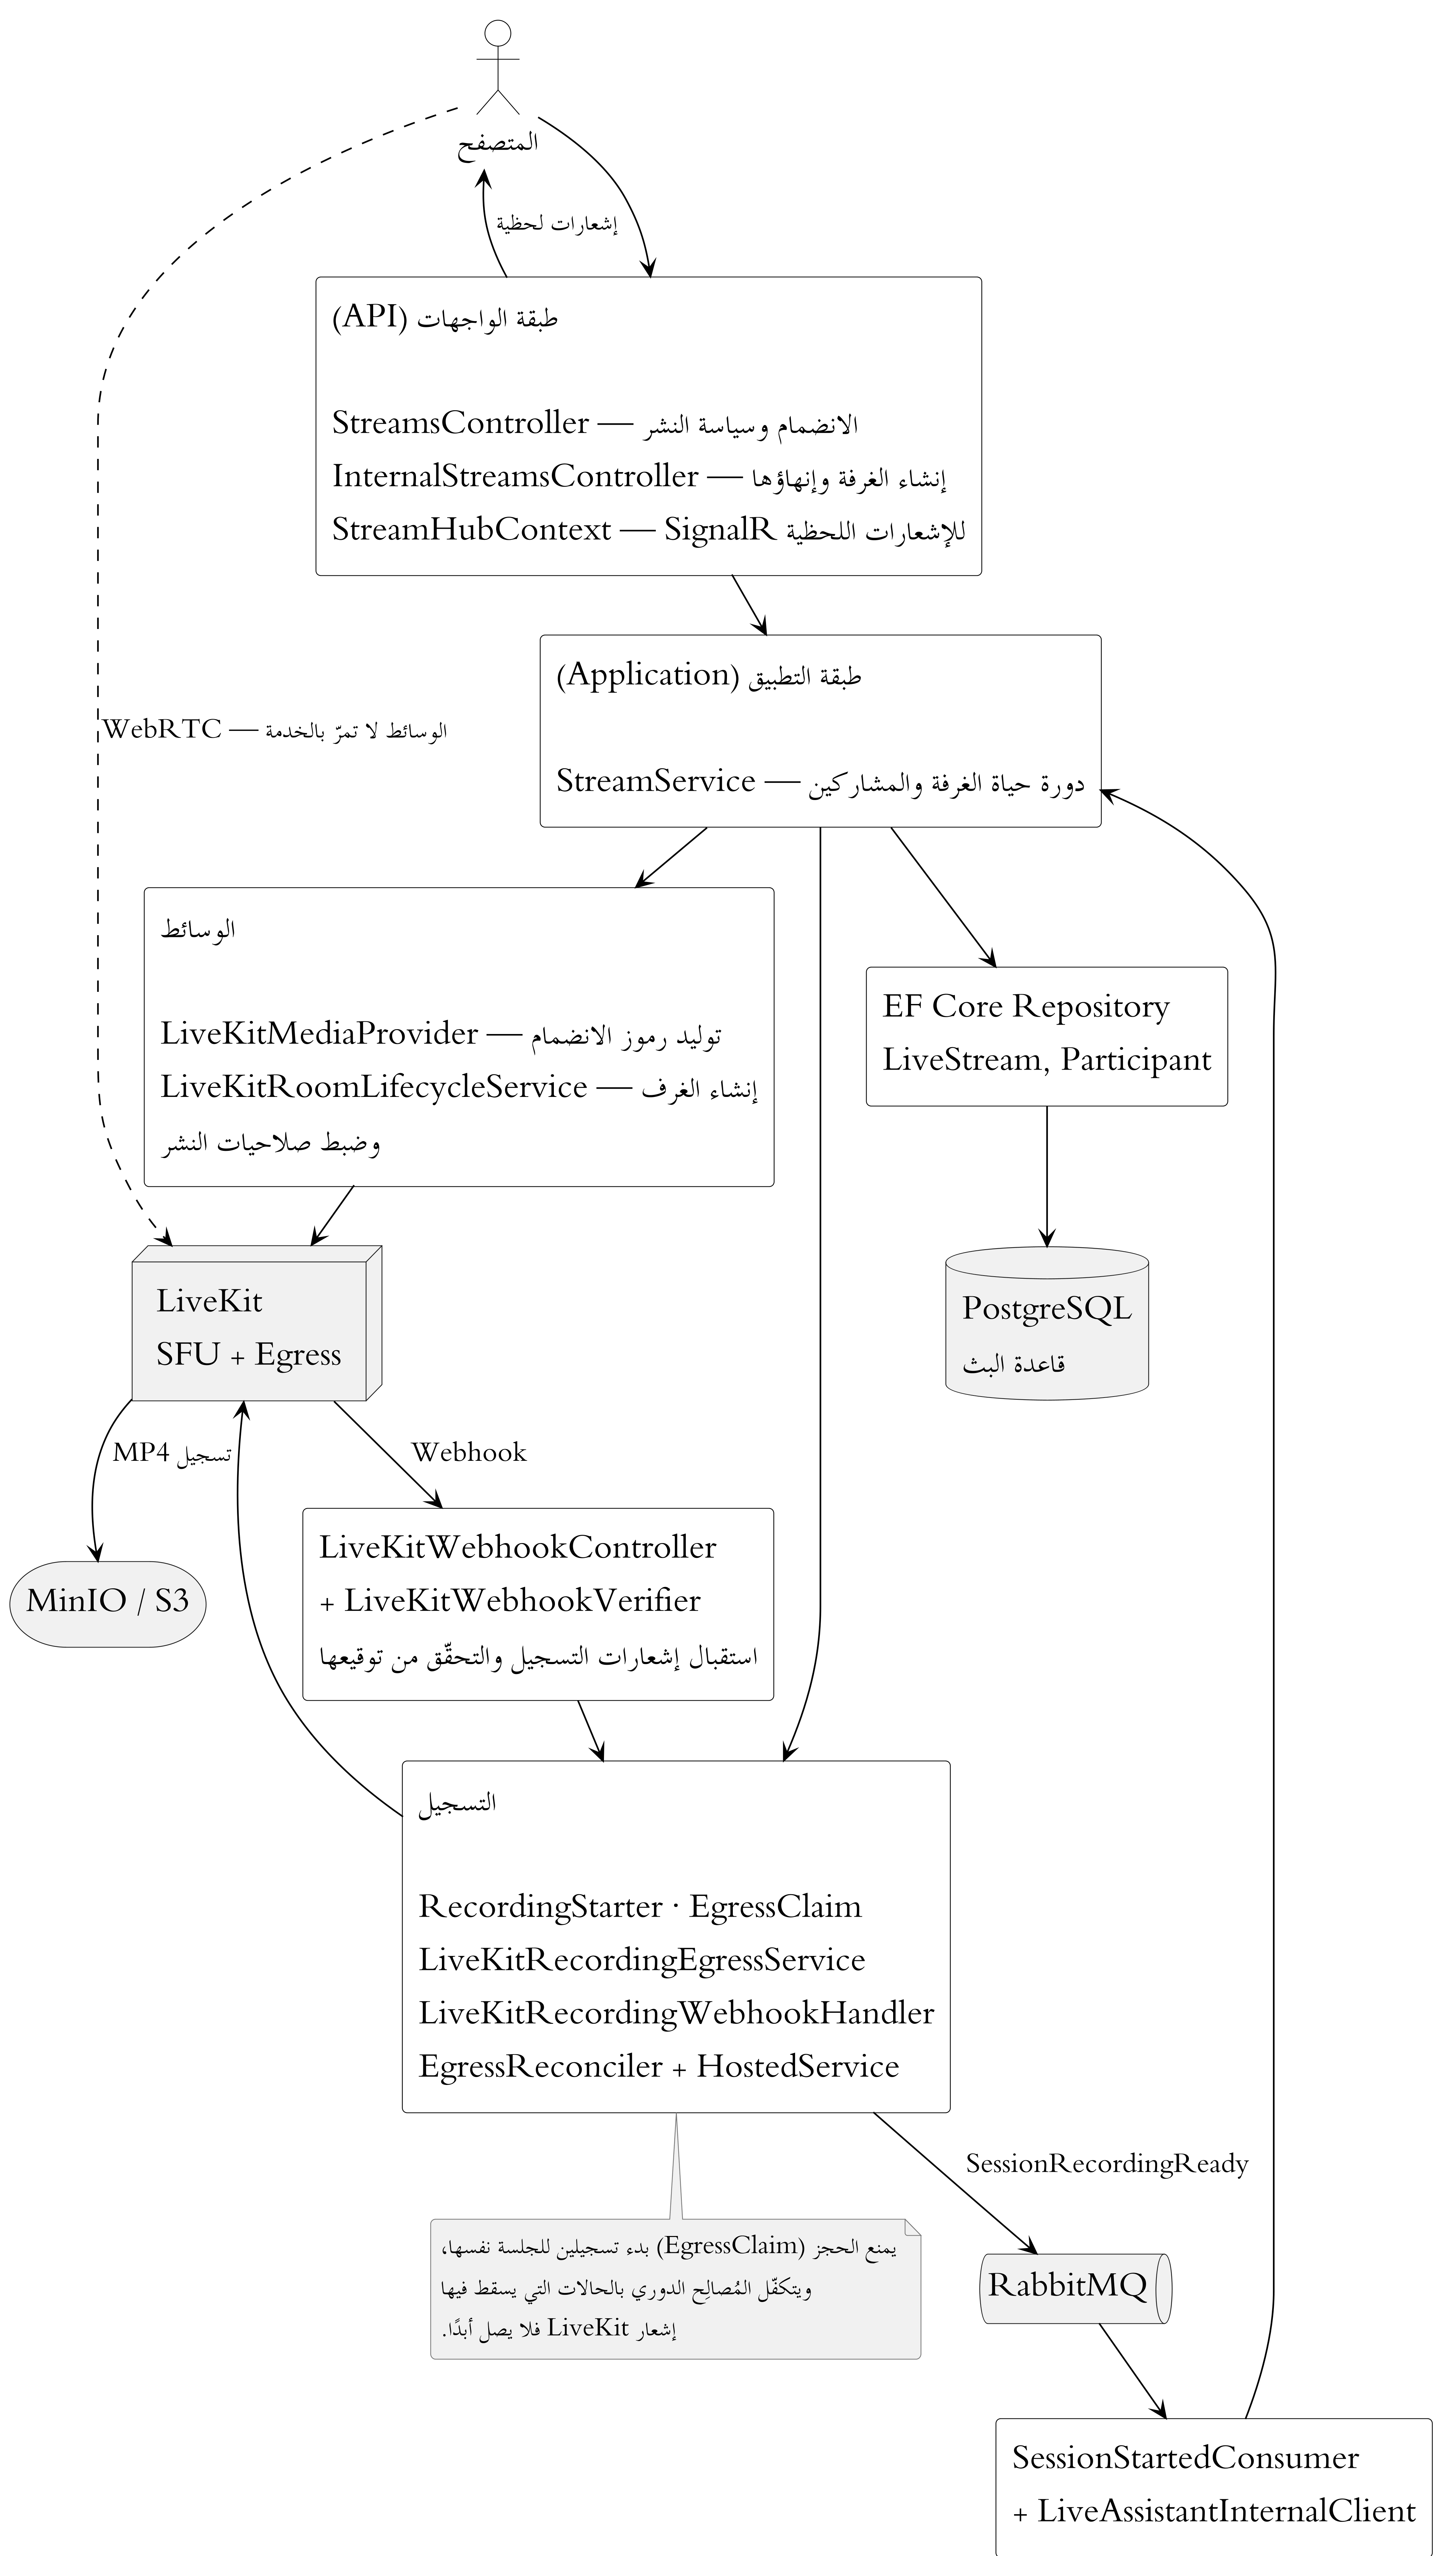
\includegraphics[width=\textwidth,height=0.8\textheight,keepaspectratio]{figures/comp-03-streaming.png}
  \caption{مخطط مكوّنات خدمة البث.}
  \label{fig:comp-03}
\end{figure}

ولا تمرّ الوسائط بالخدمة؛ إذ يتّصل المتصفّح بخادم \en{LiveKit} مباشرة عبر \en{WebRTC}، وتقتصر مهمّة الخدمة على إصدار رمز انضمام محدود الصلاحيات يحدّد ما يُسمح لصاحبه بنشره من صوت وصورة. ويمنع هذا الفصل تحوّل الخدمة إلى عنق زجاجة عند ارتفاع عدد المشاركين.

\subsection{نموذج البيانات}

يضمّ نموذج البيانات خمسة كيانات يعرضها الشكل~\ref{fig:erd-03}: البثّ الحيّ ومشاركوه، ورسائل المحادثة والأسئلة والتفاعلات المرافقة للجلسة.

% [H]: pinned under the paragraph that introduces it. Portrait at 0.90:1, so
% full width would be ~79% of the text block and could not share the page.
\begin{figure}[H]
  \centering
  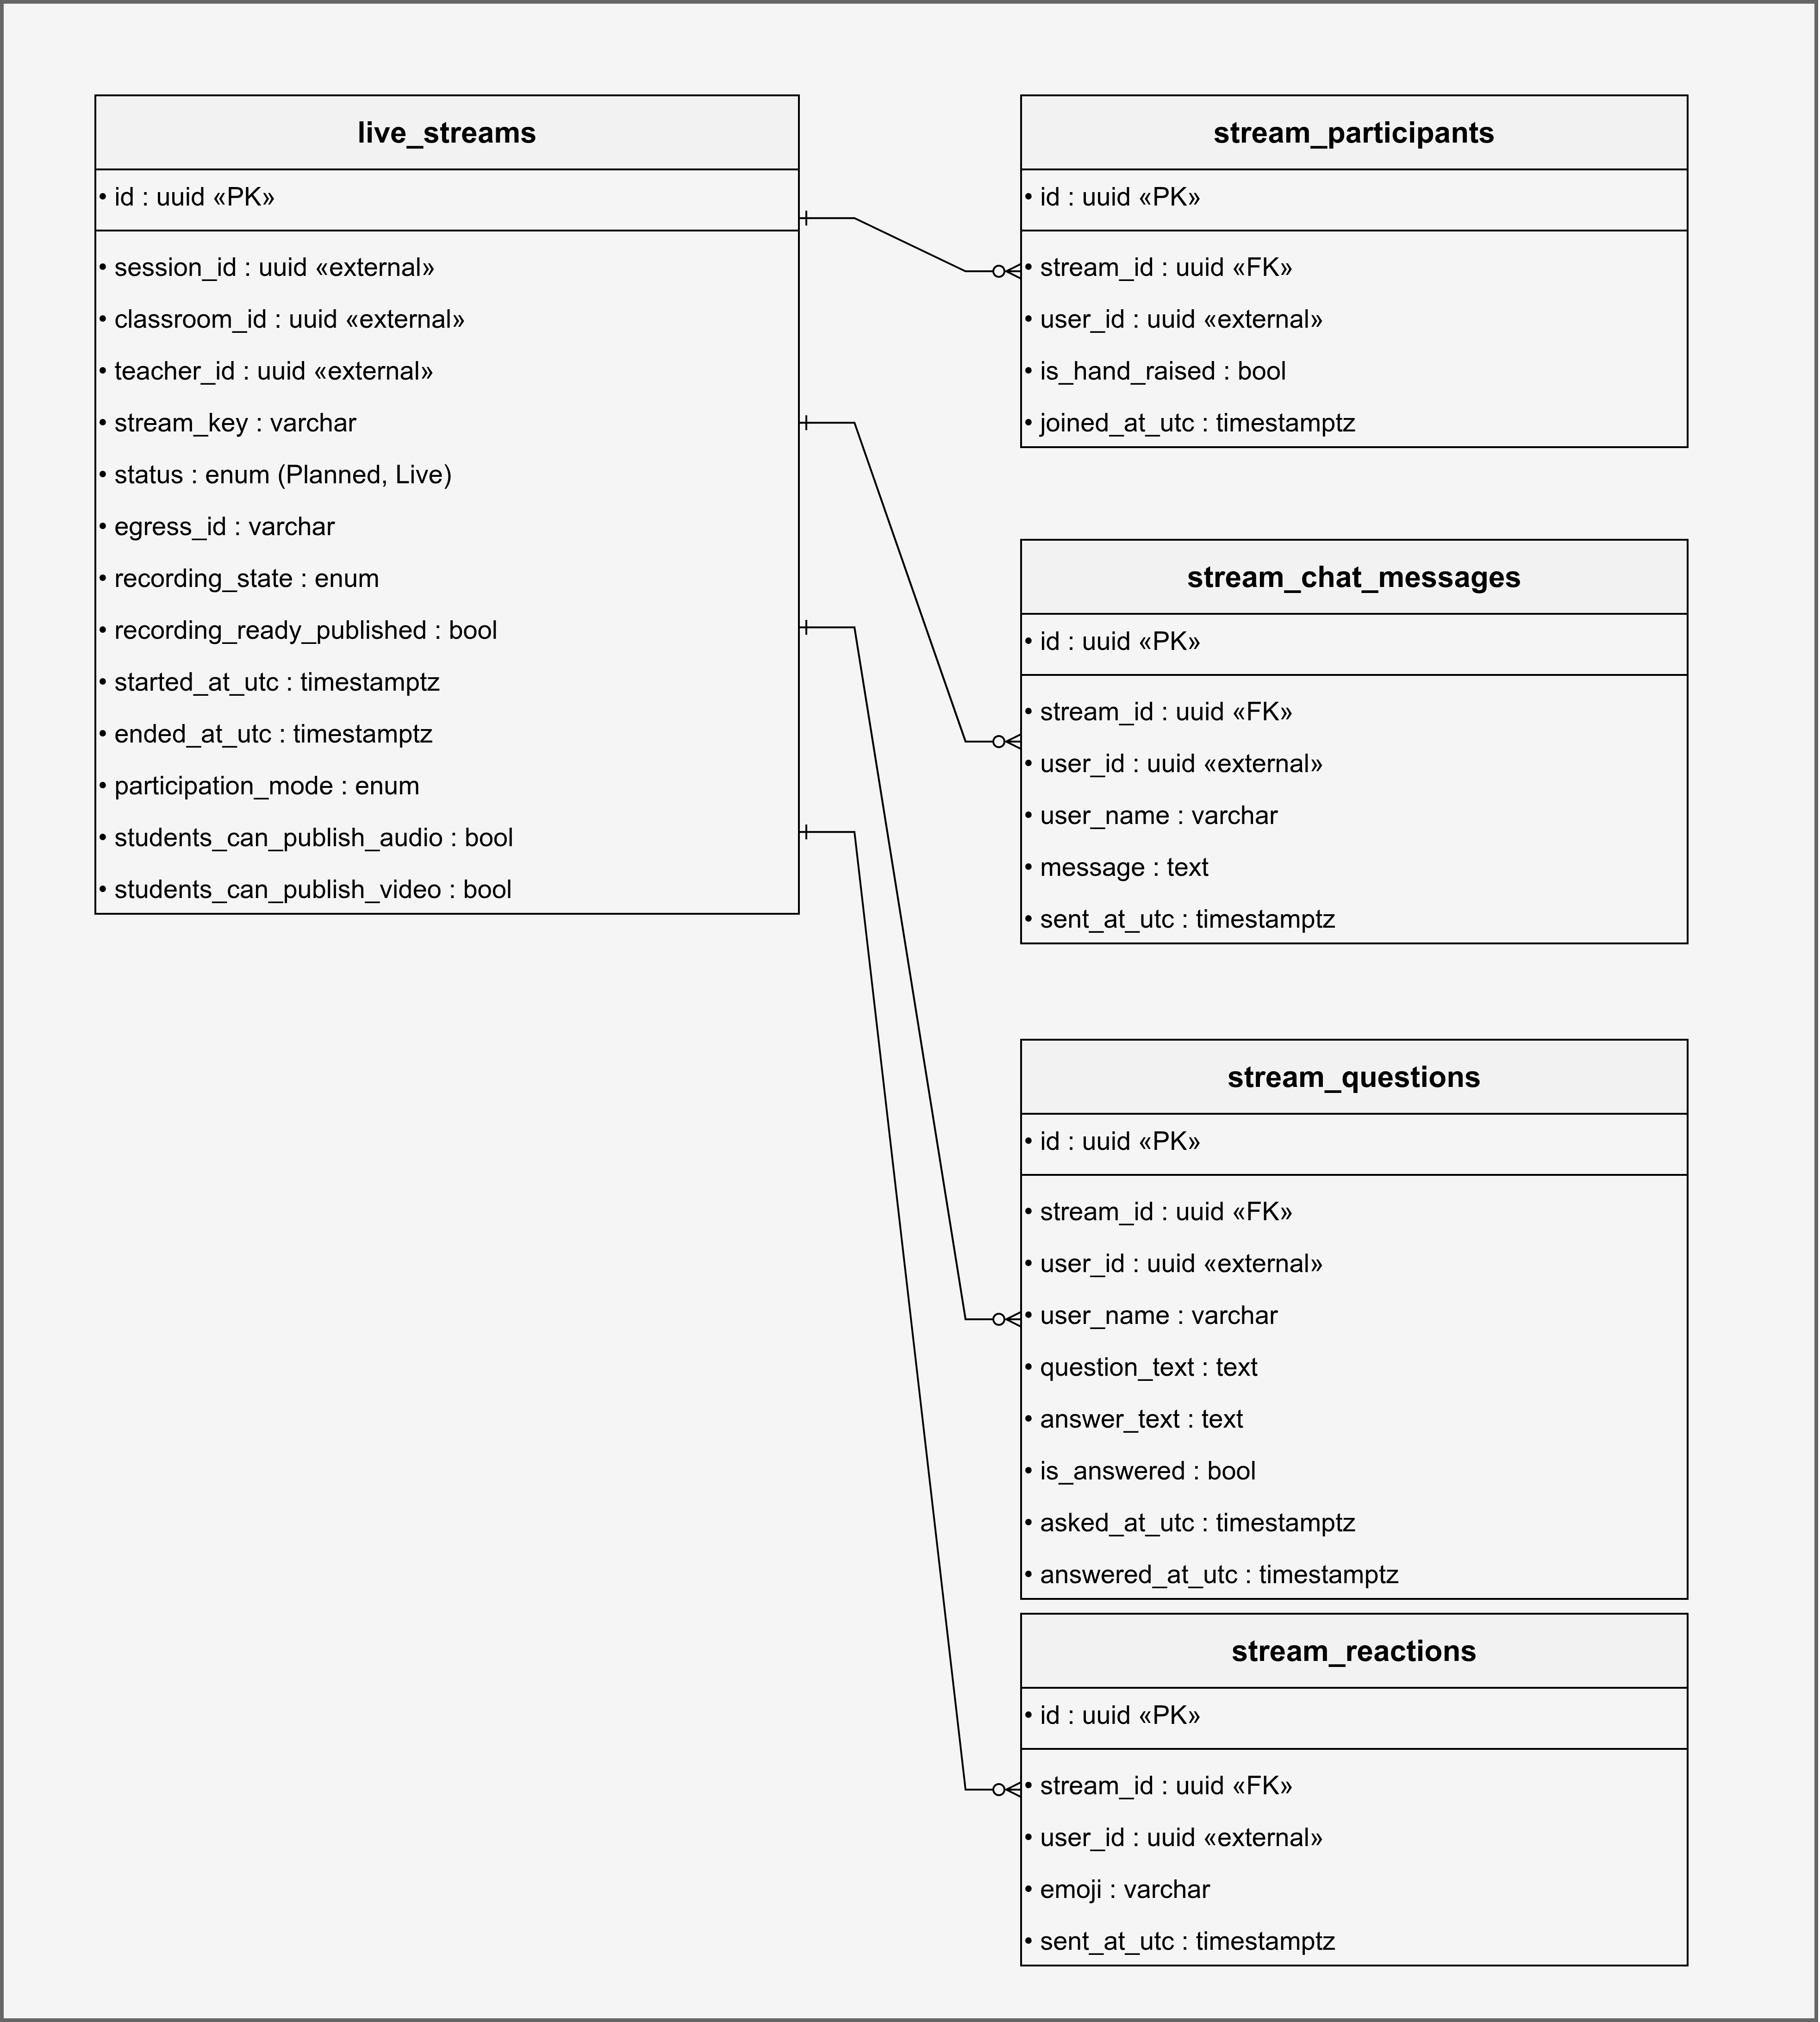
\includegraphics[width=0.55\textwidth,height=0.8\textheight,keepaspectratio]{figures/erd-03-streaming.png}
  \caption{مخطط الكيانات والعلاقات لخدمة البث.}
  \label{fig:erd-03}
\end{figure}


\section{خدمة البريد (\en{EmailService})}
% Content for Chapter 5, Section 5.7 — pulled in by chapters/05-system-design.tex
\subsection{مكوّنات الخدمة}

هي الخدمة الوحيدة في النظام التي لا تملك قاعدة بيانات ولا واجهة \en{HTTP} واردة، فهي مستهلِكة صرفة. ويعرض الشكل~\ref{fig:comp-04} مكوّناتها.

\begin{figure}[htbp]
  \centering
  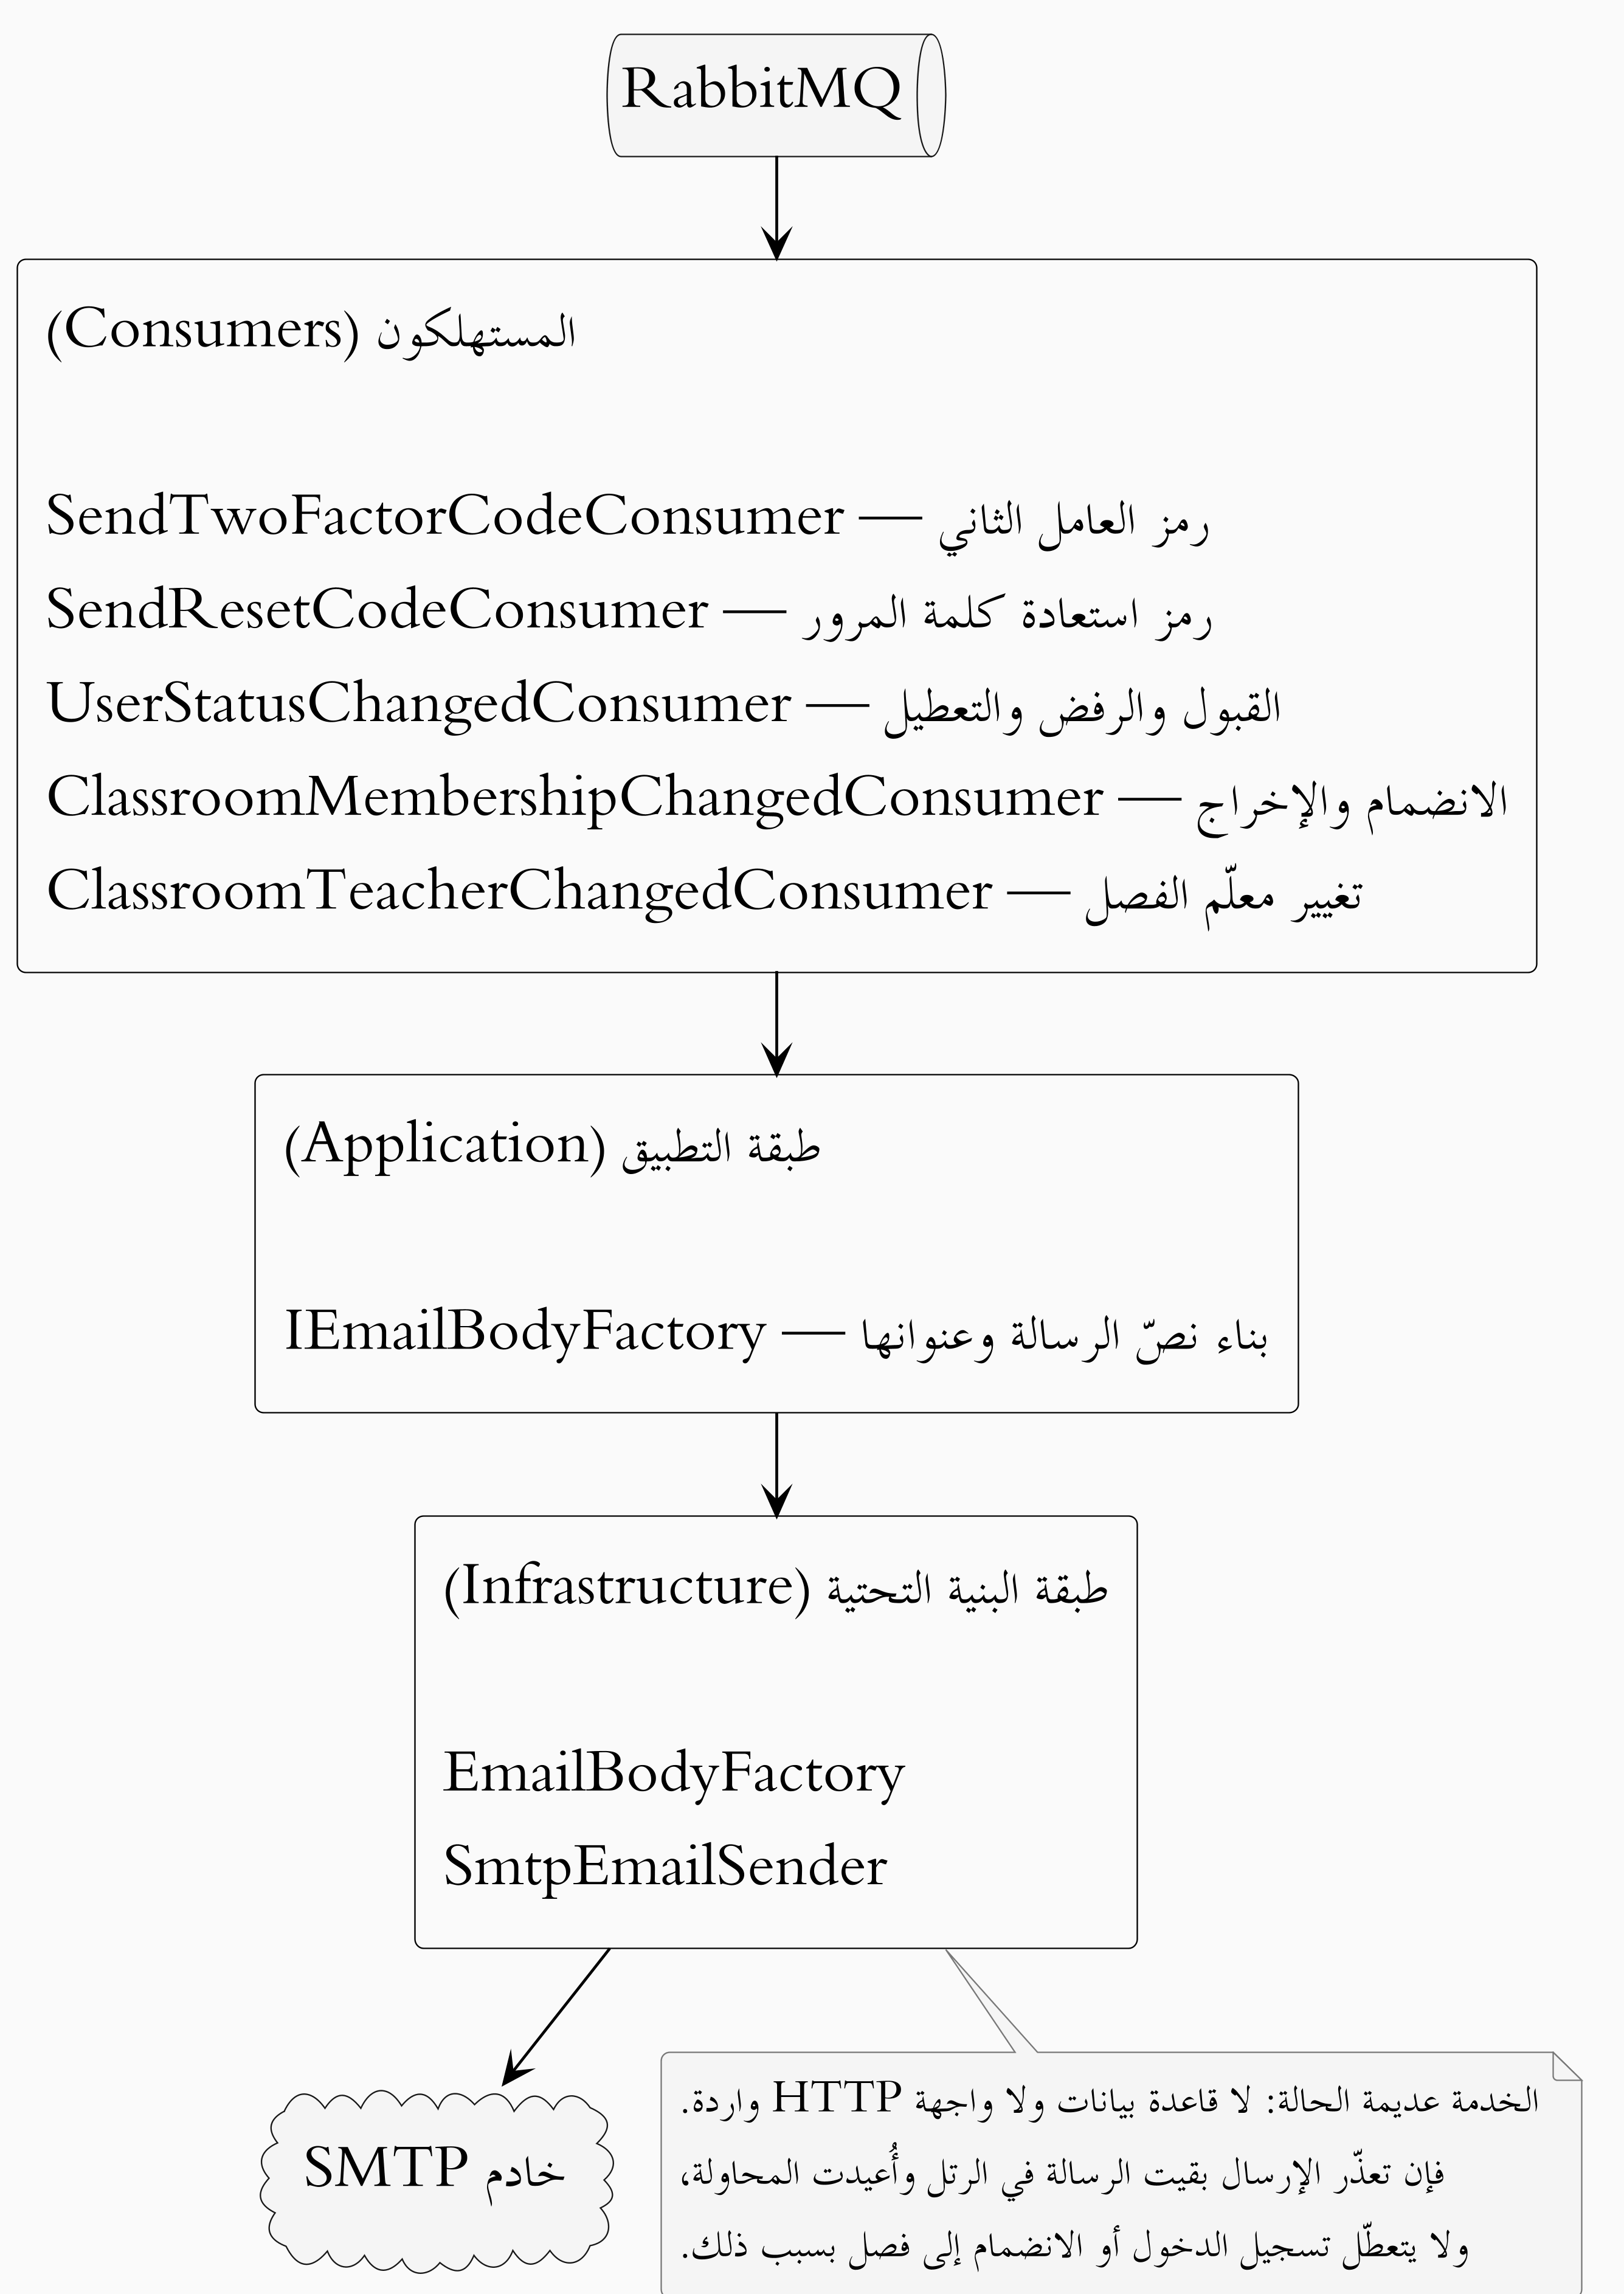
\includegraphics[width=\textwidth,height=0.8\textheight,keepaspectratio]{figures/comp-04-email.png}
  \caption{مخطط المكوّنات التفصيلي لخدمة البريد.}
  \label{fig:comp-04}
\end{figure}

ويُبيَّن مسار الإشعار من لحظة نشره إلى لحظة تسليمه، وما يحقّقه من فكِّ الارتباط الزمني، في القسم~\ref{subsubsec:flow-email}.


\section{خدمة الاسترجاع (\en{RagService})}
% Content for Chapter 5, Section 5.8 — pulled in by chapters/05-system-design.tex
\subsection{دور الخدمة ونطاقها}

% CH2-REF: originally ended "الموصوفة نظريًّا في القسم~\ref{sec:knowledge-pipeline}." — restore with chapter 2.
تحوّل خدمة المعرفة المواد المرجعية التي يرفعها المعلّم، من ملفّات \en{PDF} ومستندات \en{Word} وعروض \en{PowerPoint}، إلى قاعدة معرفية قابلة للبحث الدلالي تغذّي قدرات التوليد المعزّز بالاسترجاع (\en{RAG}). وتنفّذ الخدمة مرحلتين: الفهرسة (\en{Indexing}) والاسترجاع (\en{Retrieval})، فيُبنى فهرس دلالي لكل فصل دراسي تُؤصَّل به إجابات النظام في مادة ذلك الفصل.

\subsection{مكوّنات الخدمة}

يعرض الشكل~\ref{fig:comp-05} مكوّنات الخدمة وروابطها الخارجية، وهي مجمّعة بحسب المهامّ الأربع التي تؤدّيها: الاستيعاب والاسترجاع والتلخيص وإعادة التضمين.

\begin{figure}[htbp]
  \centering
  % Width to be re-checked when the draw.io export replaces this PNG.
  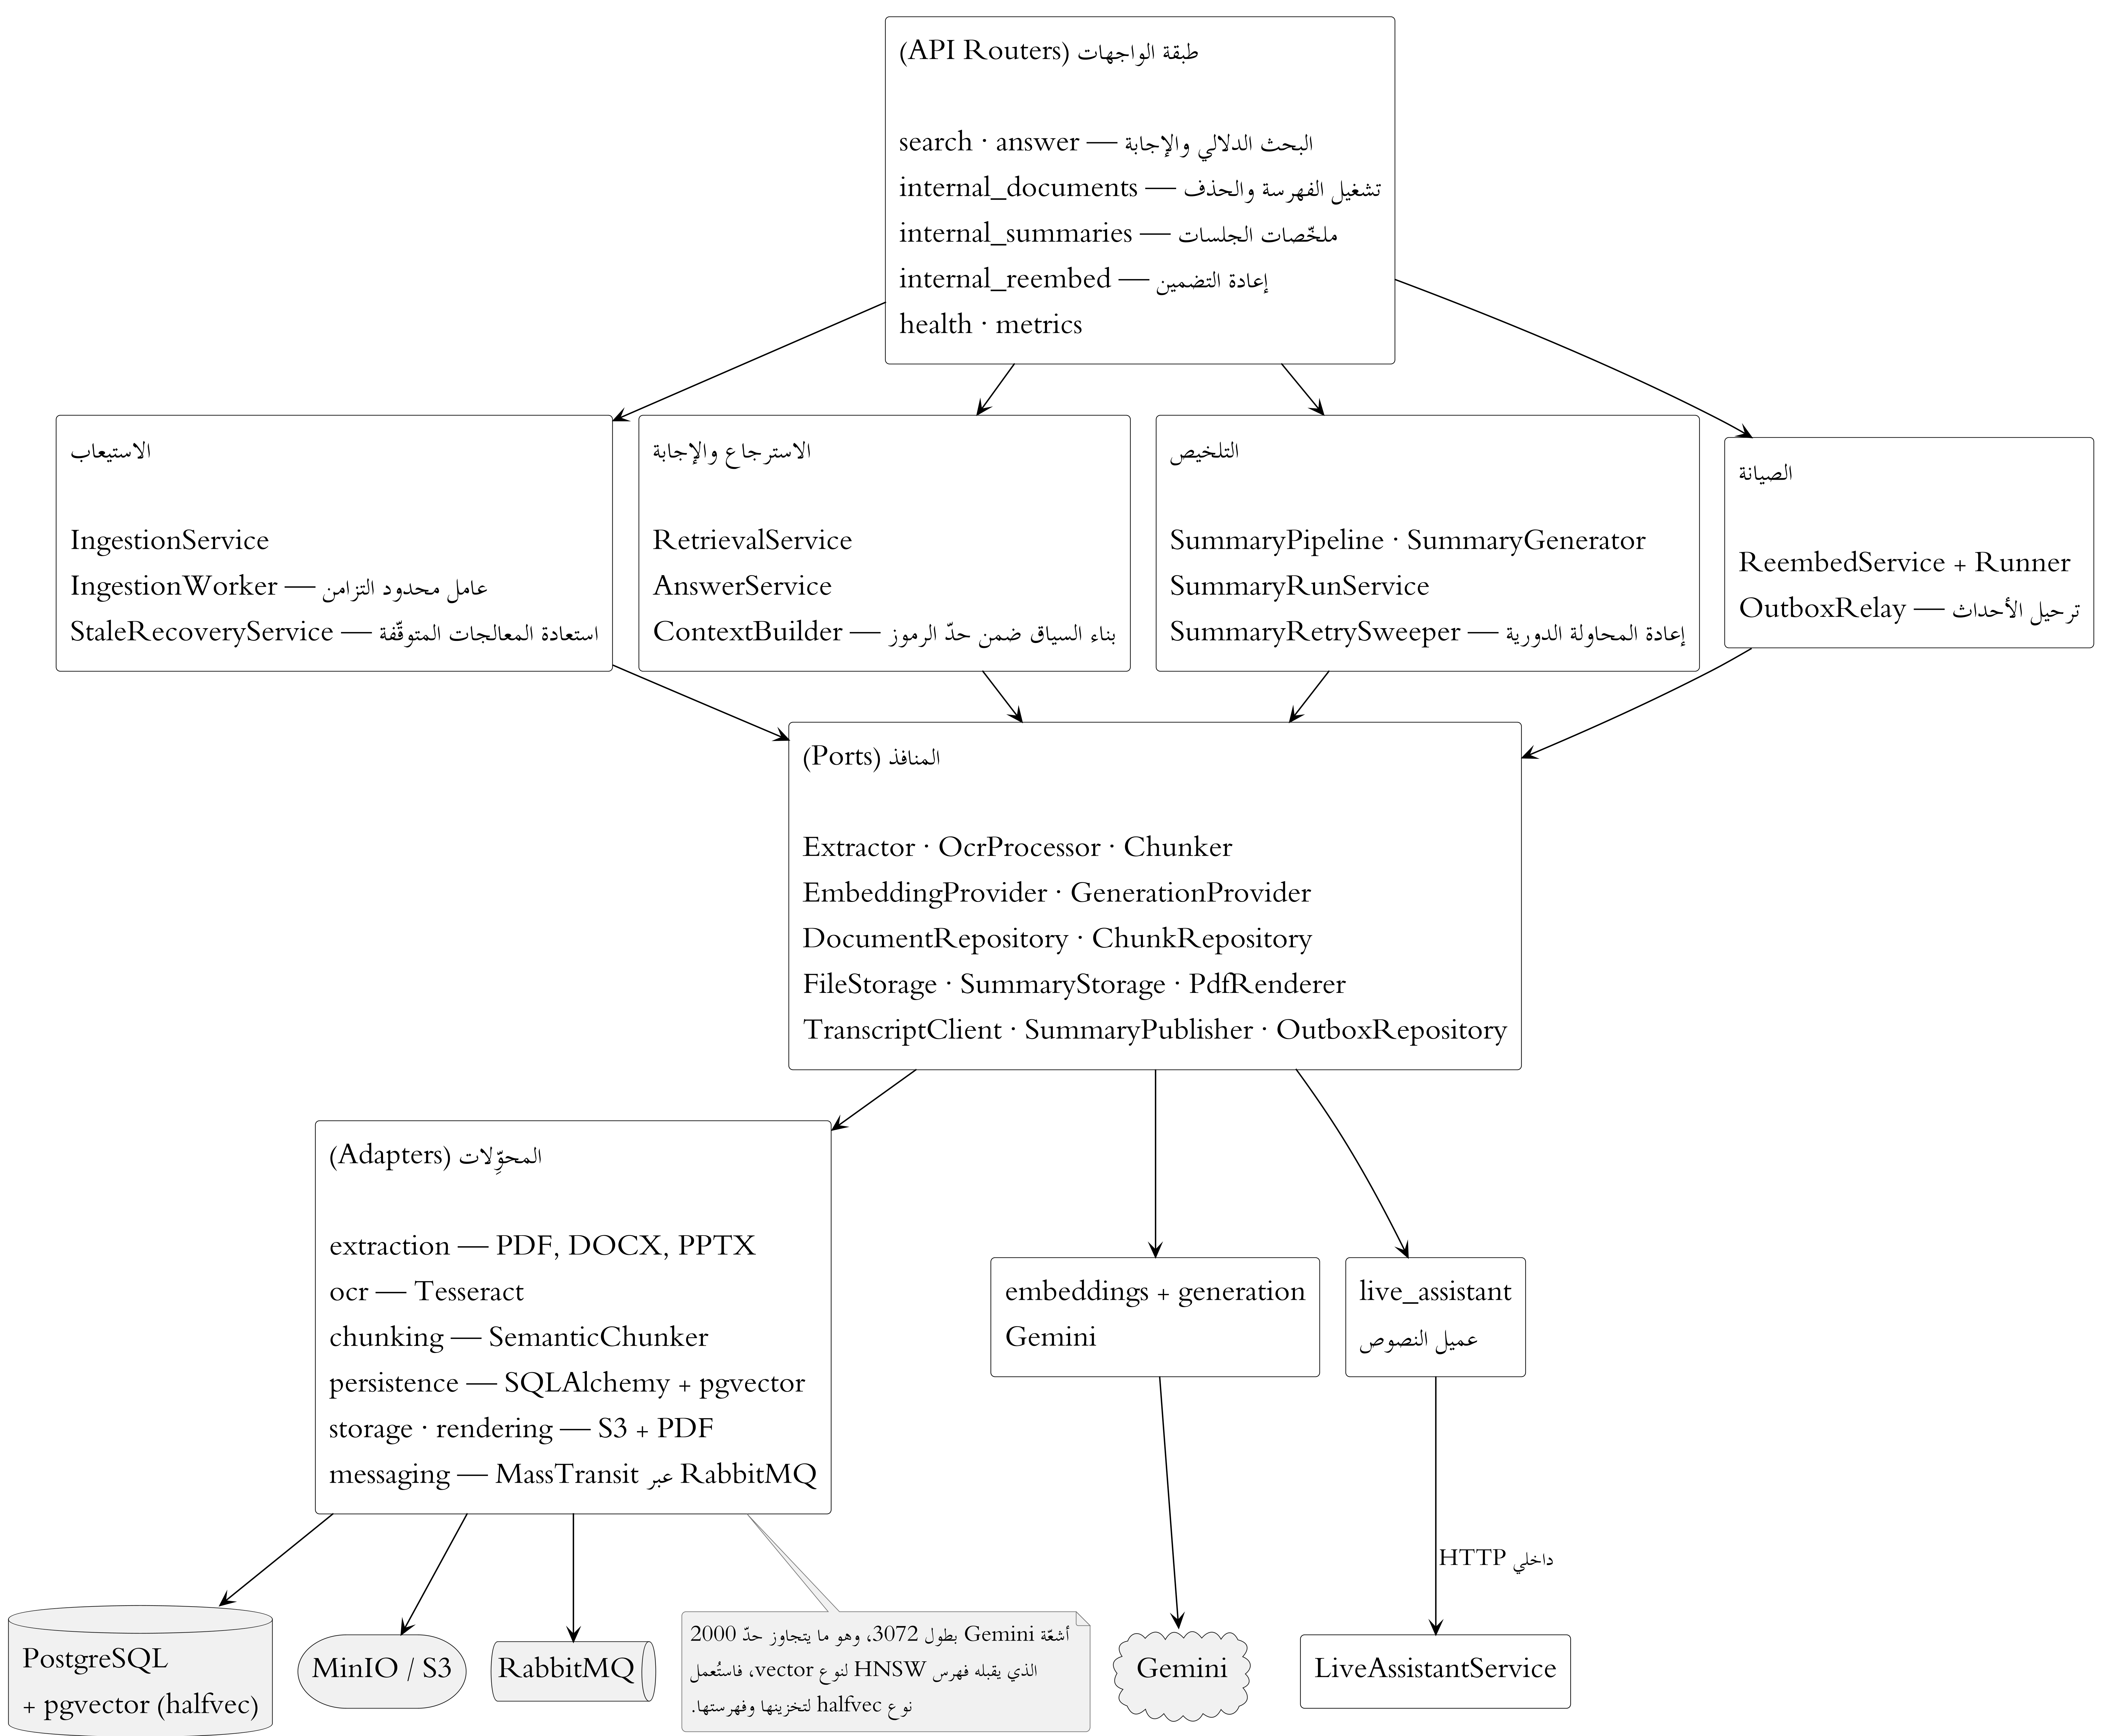
\includegraphics[width=\textwidth,height=0.8\textheight,keepaspectratio]{figures/comp-05-rag.png}
  \caption{مخطط مكوّنات خدمة المعرفة.}
  \label{fig:comp-05}
\end{figure}

وطُبّق في هذه الخدمة نمط المنافذ والمحوِّلات: تُعرّف طبقة التطبيق منافذ مجرّدة تصف ما تحتاجه الخدمة من استخراج وتضمين وتخزين، ويقع كل اختيار تقني خلف أحدها في طبقة البنية التحتية. ويحصر ذلك استبدال مزوّد التضمين أو محرّك التعرّف الضوئي في محوِّل واحد، دون تعديل منطق خط الأنابيب. ويعرض الشكل~\ref{fig:class-01} هذا التصميم مطبَّقاً على خط أنابيب الاستيعاب.

\begin{figure}[htbp]
  \centering
  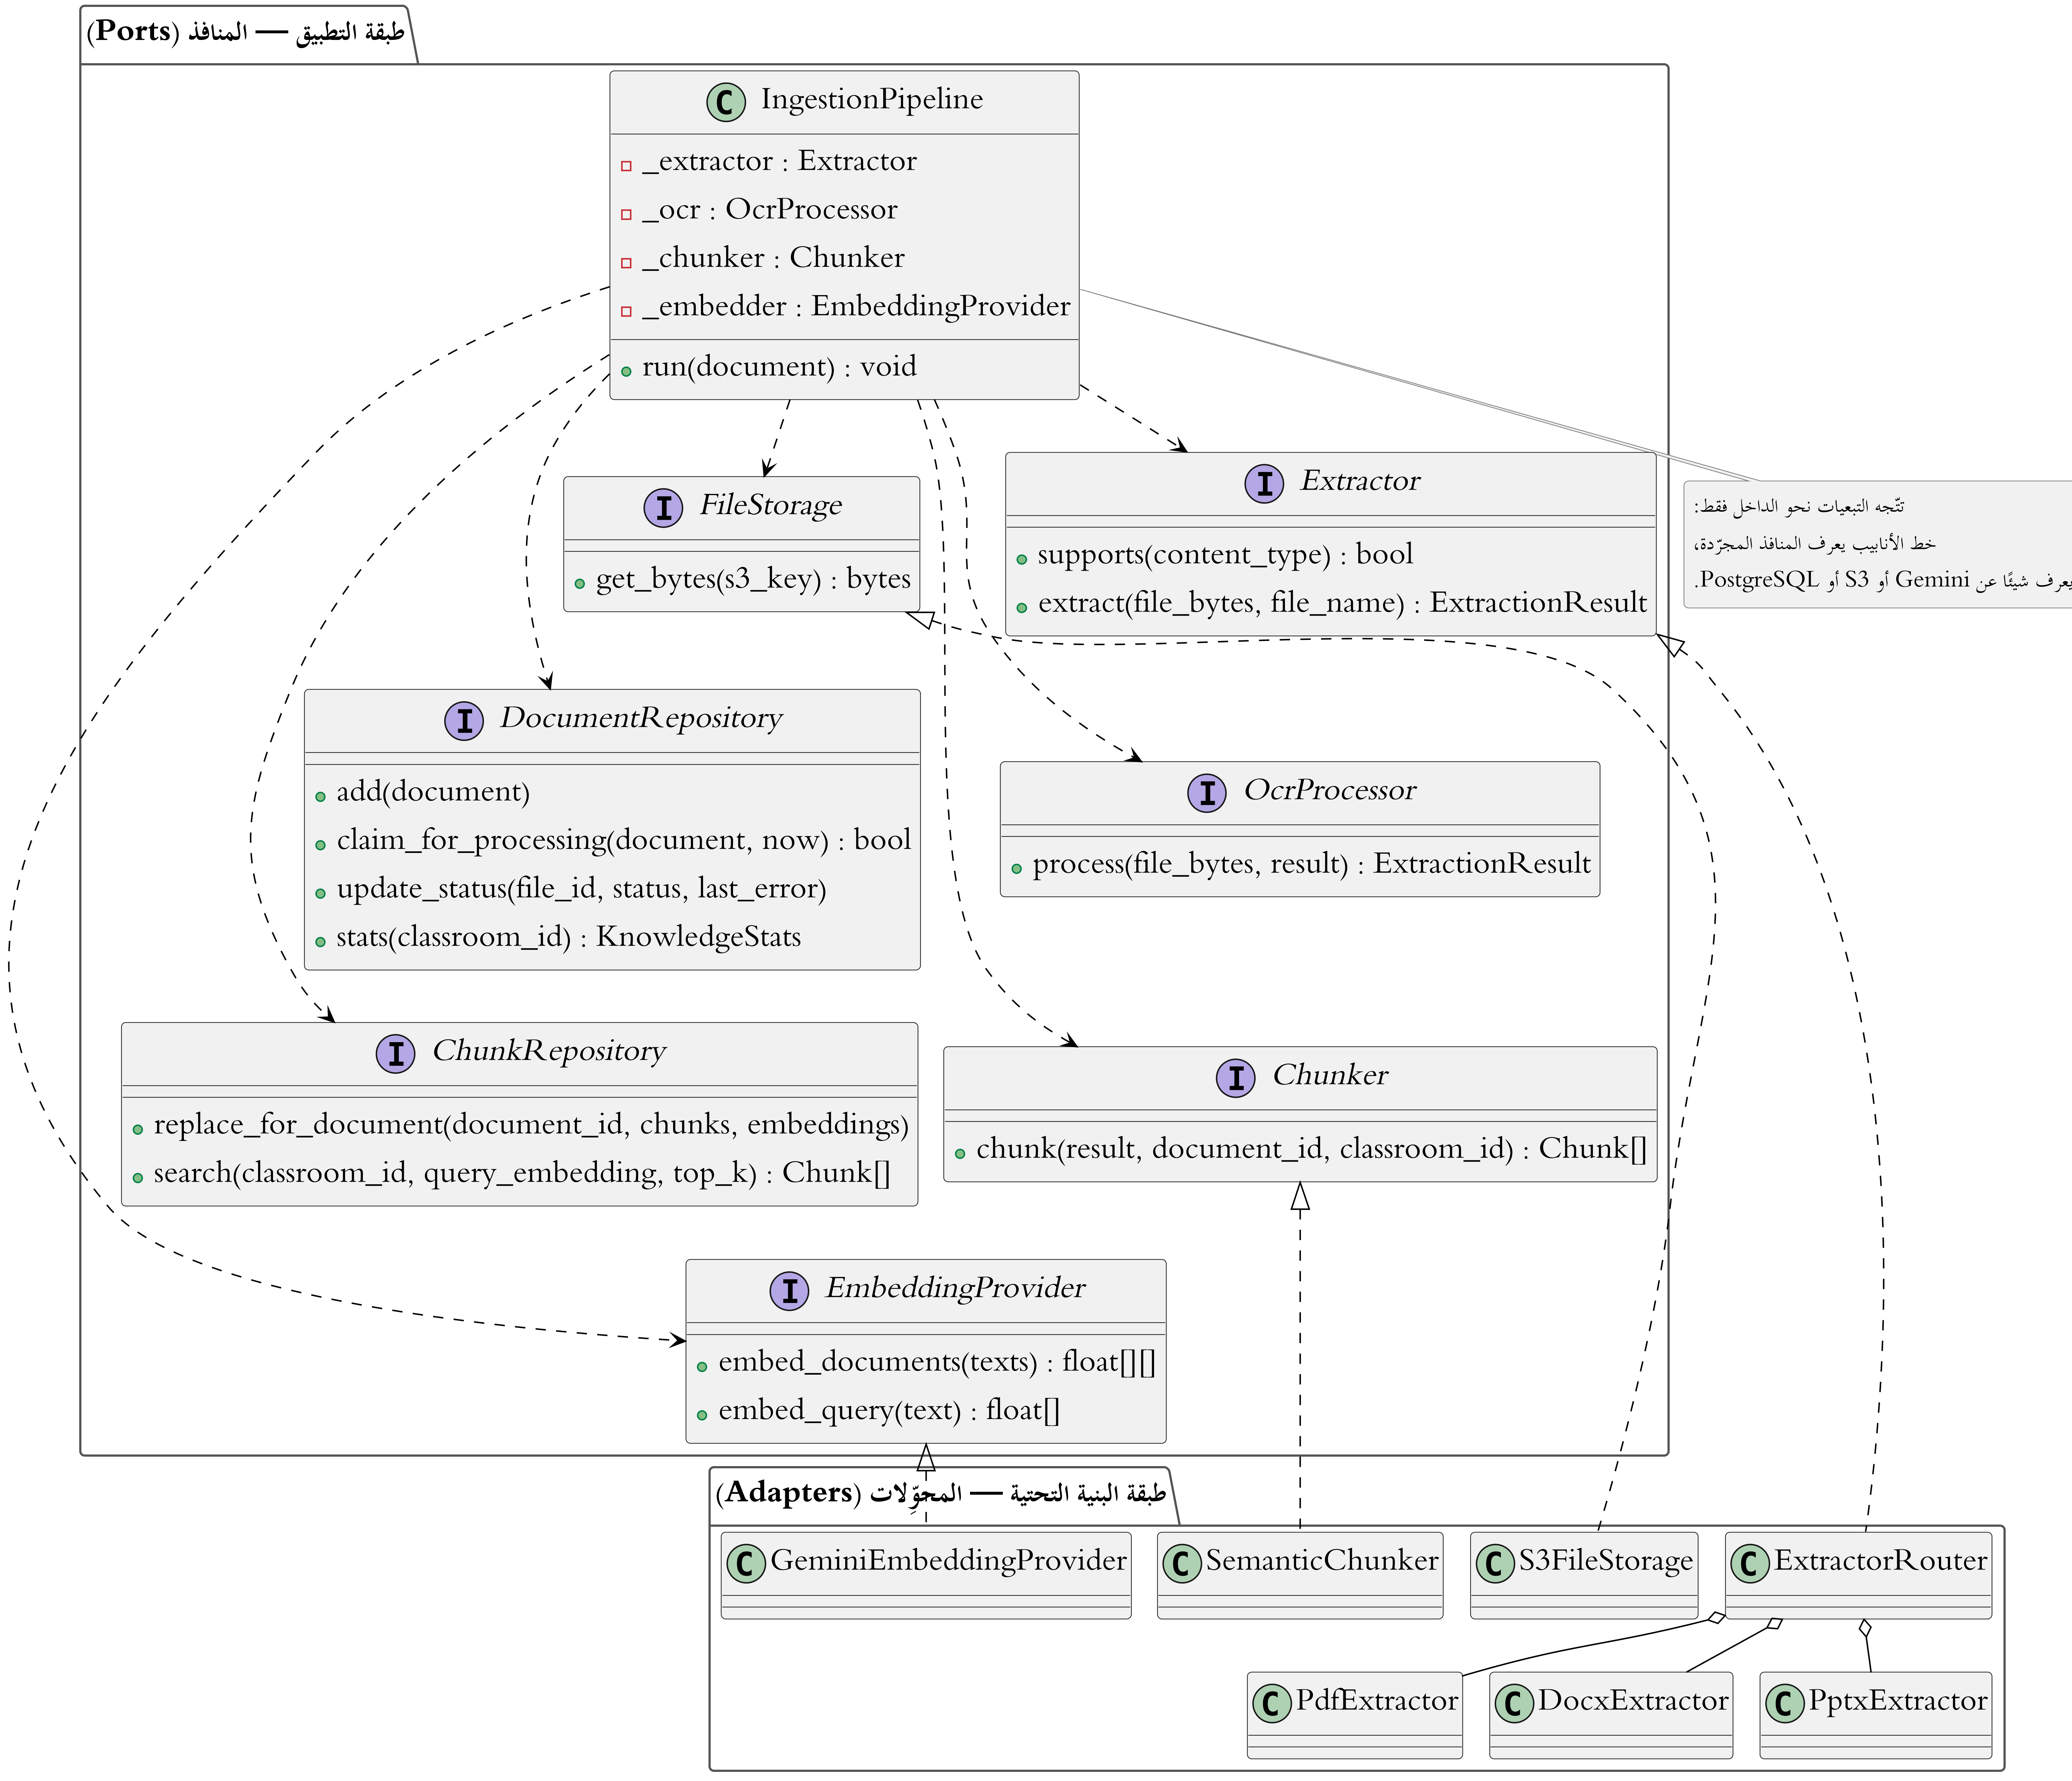
\includegraphics[width=\textwidth,height=0.8\textheight,keepaspectratio]{figures/class-01-ports-adapters.png}
  \caption{مخطط الصفوف لنمط المنافذ والمحوِّلات في خط أنابيب الاستيعاب.}
  \label{fig:class-01}
\end{figure}

\subsection{نموذج البيانات}
\label{subsec:rag-data-model}

يقوم نموذج البيانات على أربعة كيانات يعرضها الشكل~\ref{fig:erd-04}: المستند والمقطع، وسجلّات محاولات التلخيص، وجدول صندوق الصادر.

\begin{figure}[htbp]
  \centering
  % Width to be re-checked when the draw.io export replaces this PNG.
  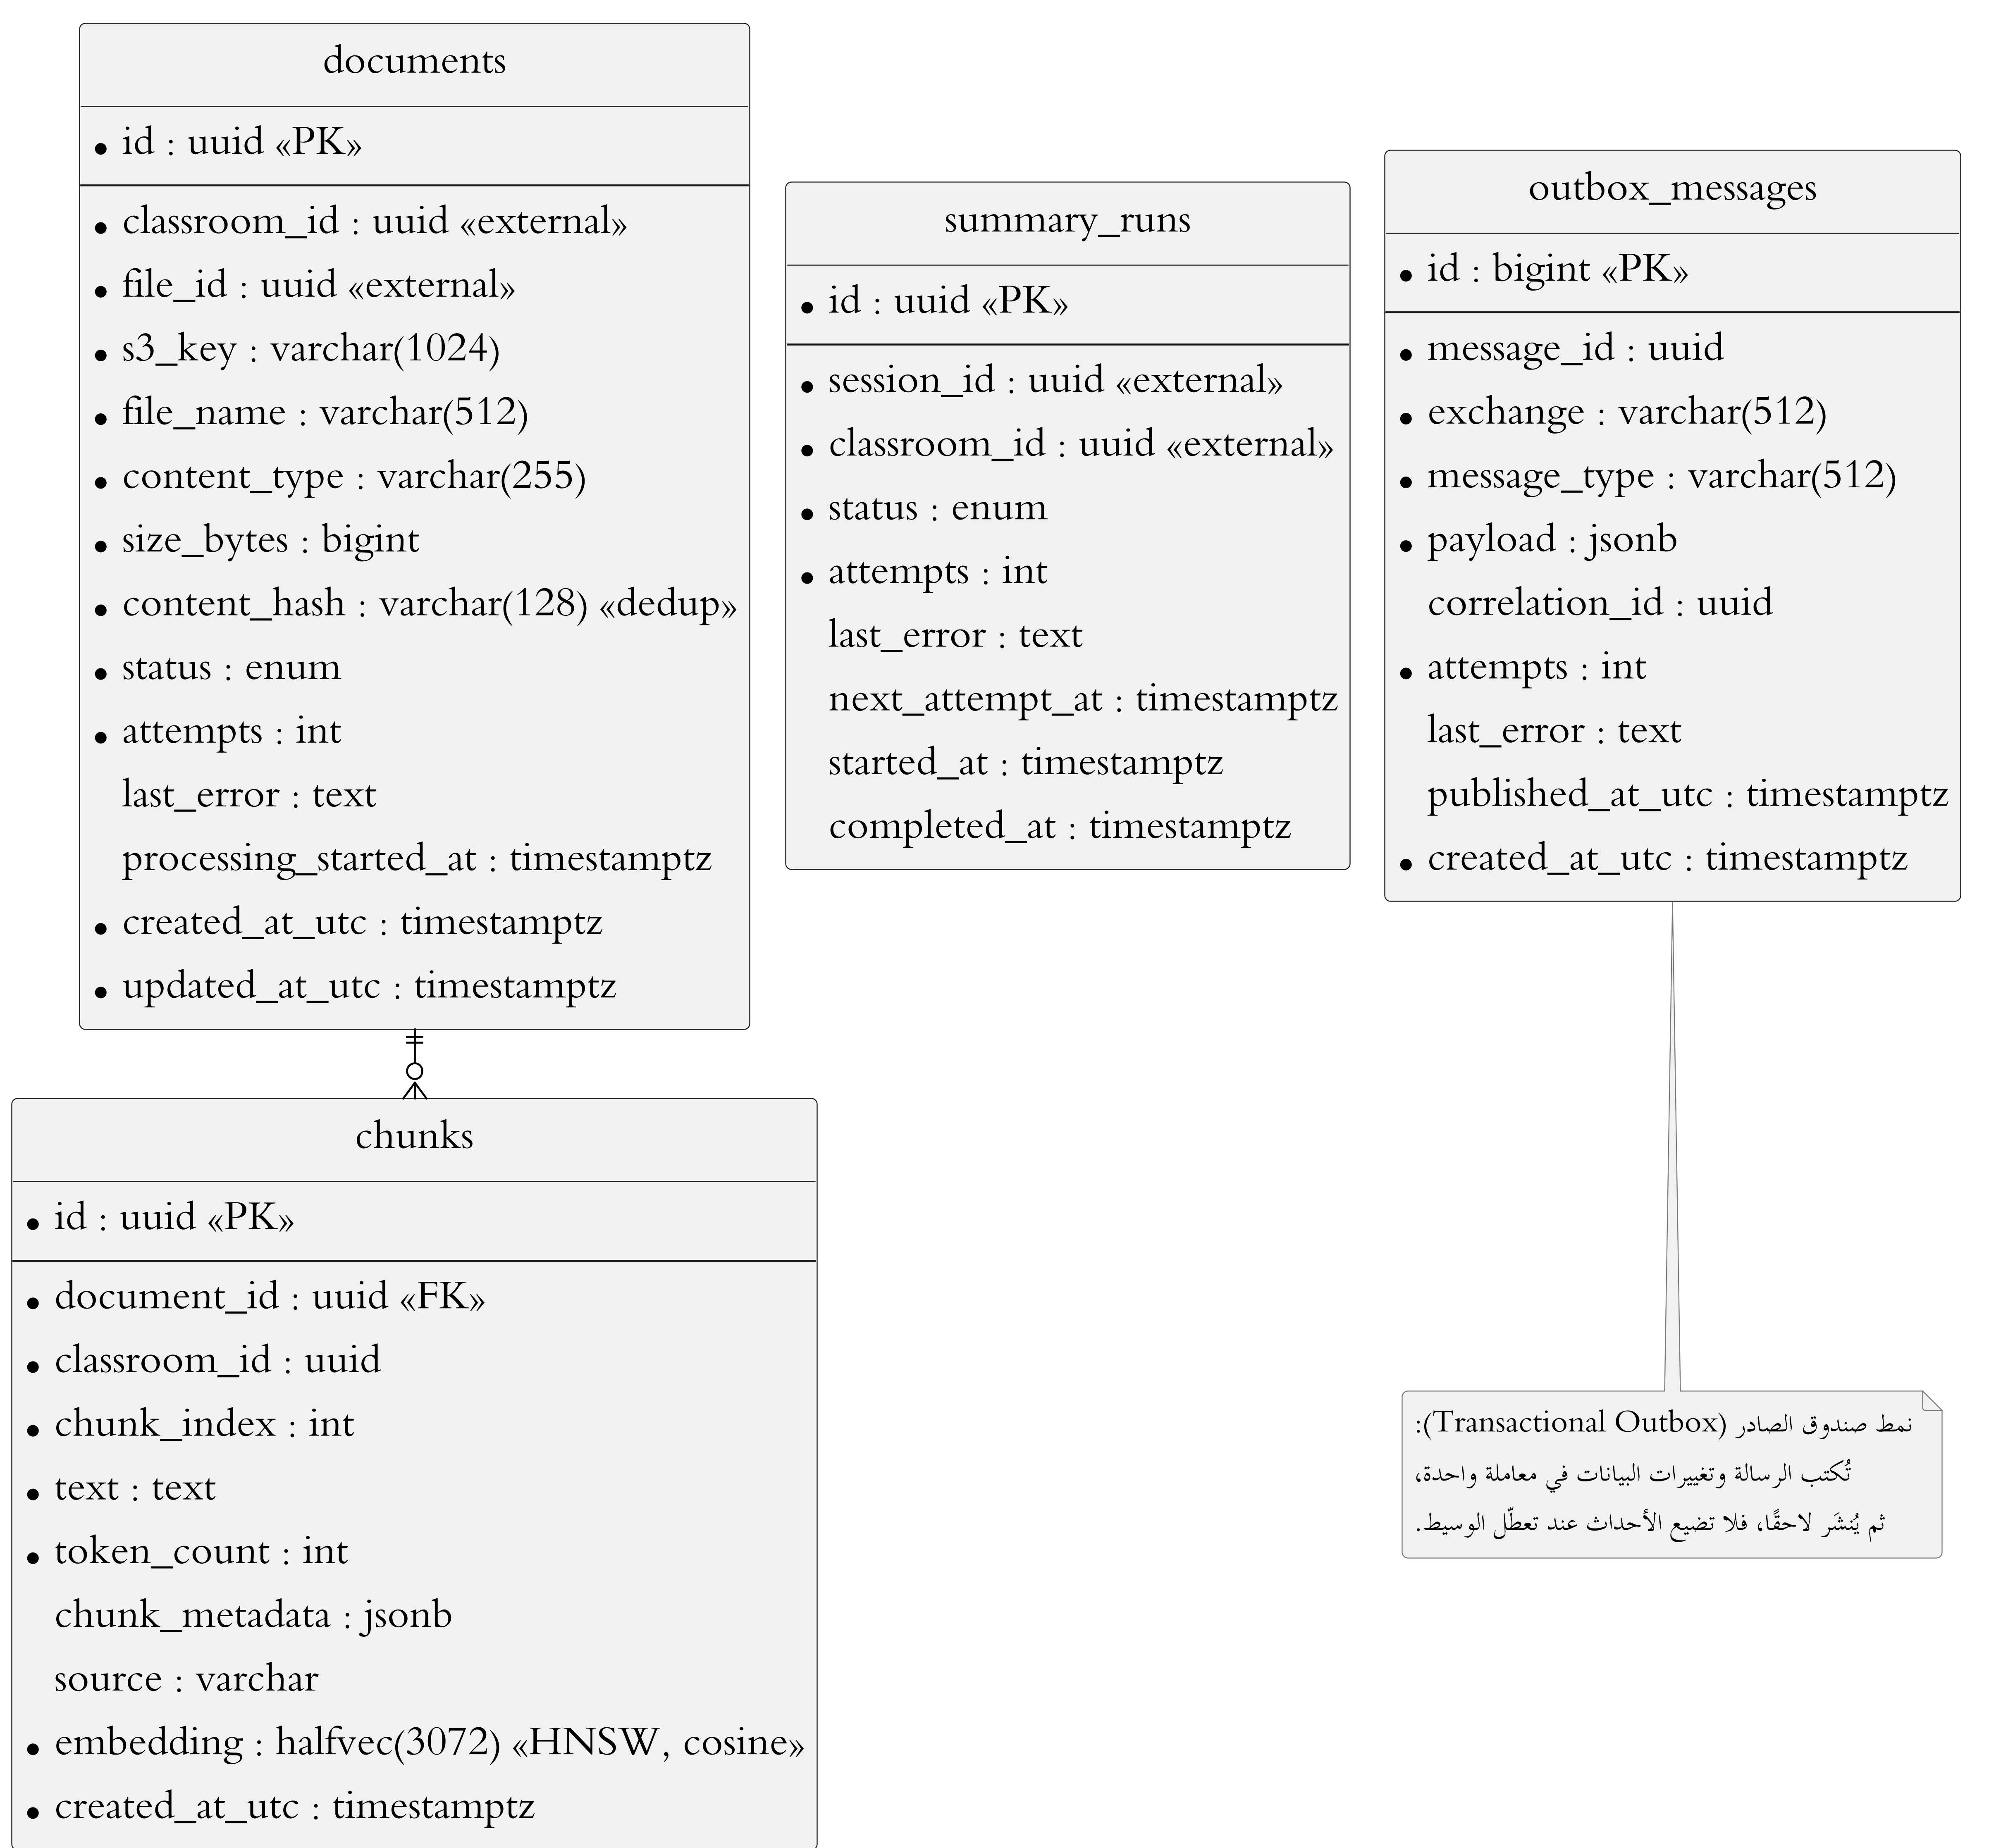
\includegraphics[width=\textwidth,height=0.8\textheight,keepaspectratio]{figures/erd-04-rag.png}
  \caption{مخطط الكيانات والعلاقات لخدمة المعرفة.}
  \label{fig:erd-04}
\end{figure}

ويتضمّن هذا النموذج قرارين تصميميين:

\begin{enumerate}
  \item \textbf{تضمين معرّف الفصل في كيان المقطع}: يتيح قصر البحث الدلالي على فصل بعينه، فيُعزَل محتوى كل فصل ولا يتسرّب إلى نتائج فصل آخر.
  \item \textbf{استعمال النوع \en{halfvec} لتخزين الأشعّة}: يبلغ طول شعاع التضمين 3072، وهو يتجاوز الحدّ الأقصى البالغ 2000 الذي يقبله فهرس \en{HNSW} للنوع \en{vector}. ويقبل النوع \en{halfvec} هذا الطول ويسمح بفهرسته.
\end{enumerate}


\section{خدمة المساعد المباشر (\en{LiveAssistantService})}
% Content for Chapter 5, Section 5.9 — pulled in by chapters/05-system-design.tex
\subsection{دور الخدمة ونطاقها}

تتابع هذه الخدمة الشرح أثناء الجلسة الحيّة، فتحوّل صوت المعلّم إلى نصّ، وتقارن ما يشرحه بالمادة المرجعية المفهرسة، وترسل إليه ملاحظة خاصّة عند رصد فرق أو نقص. وهي الخدمة الوحيدة التي يقوم مسارها الرئيس على حلقة مستمرّة تعمل طوال الجلسة، لا على دورة طلب وجواب.

\subsection{مكوّنات الخدمة}

تنتظم مكوّنات طبقة التطبيق مراحلَ متتابعة تمثّل هذه الحلقة: التقاط الصوت، وتحويله إلى نصّ، وكشف حدّ الفكرة، وتقييمها مقابل المصادر، وضبط إيقاع التدخّل، ثمّ إرساله. ويعرض الشكل~\ref{fig:comp-06} هذه المكوّنات وروابطها الخارجية.

% [H]: pinned under the paragraph that introduces it. At 2.09:1 full width is
% only ~32% of the text block, so it fits without shrinking.
\begin{figure}[H]
  \centering
  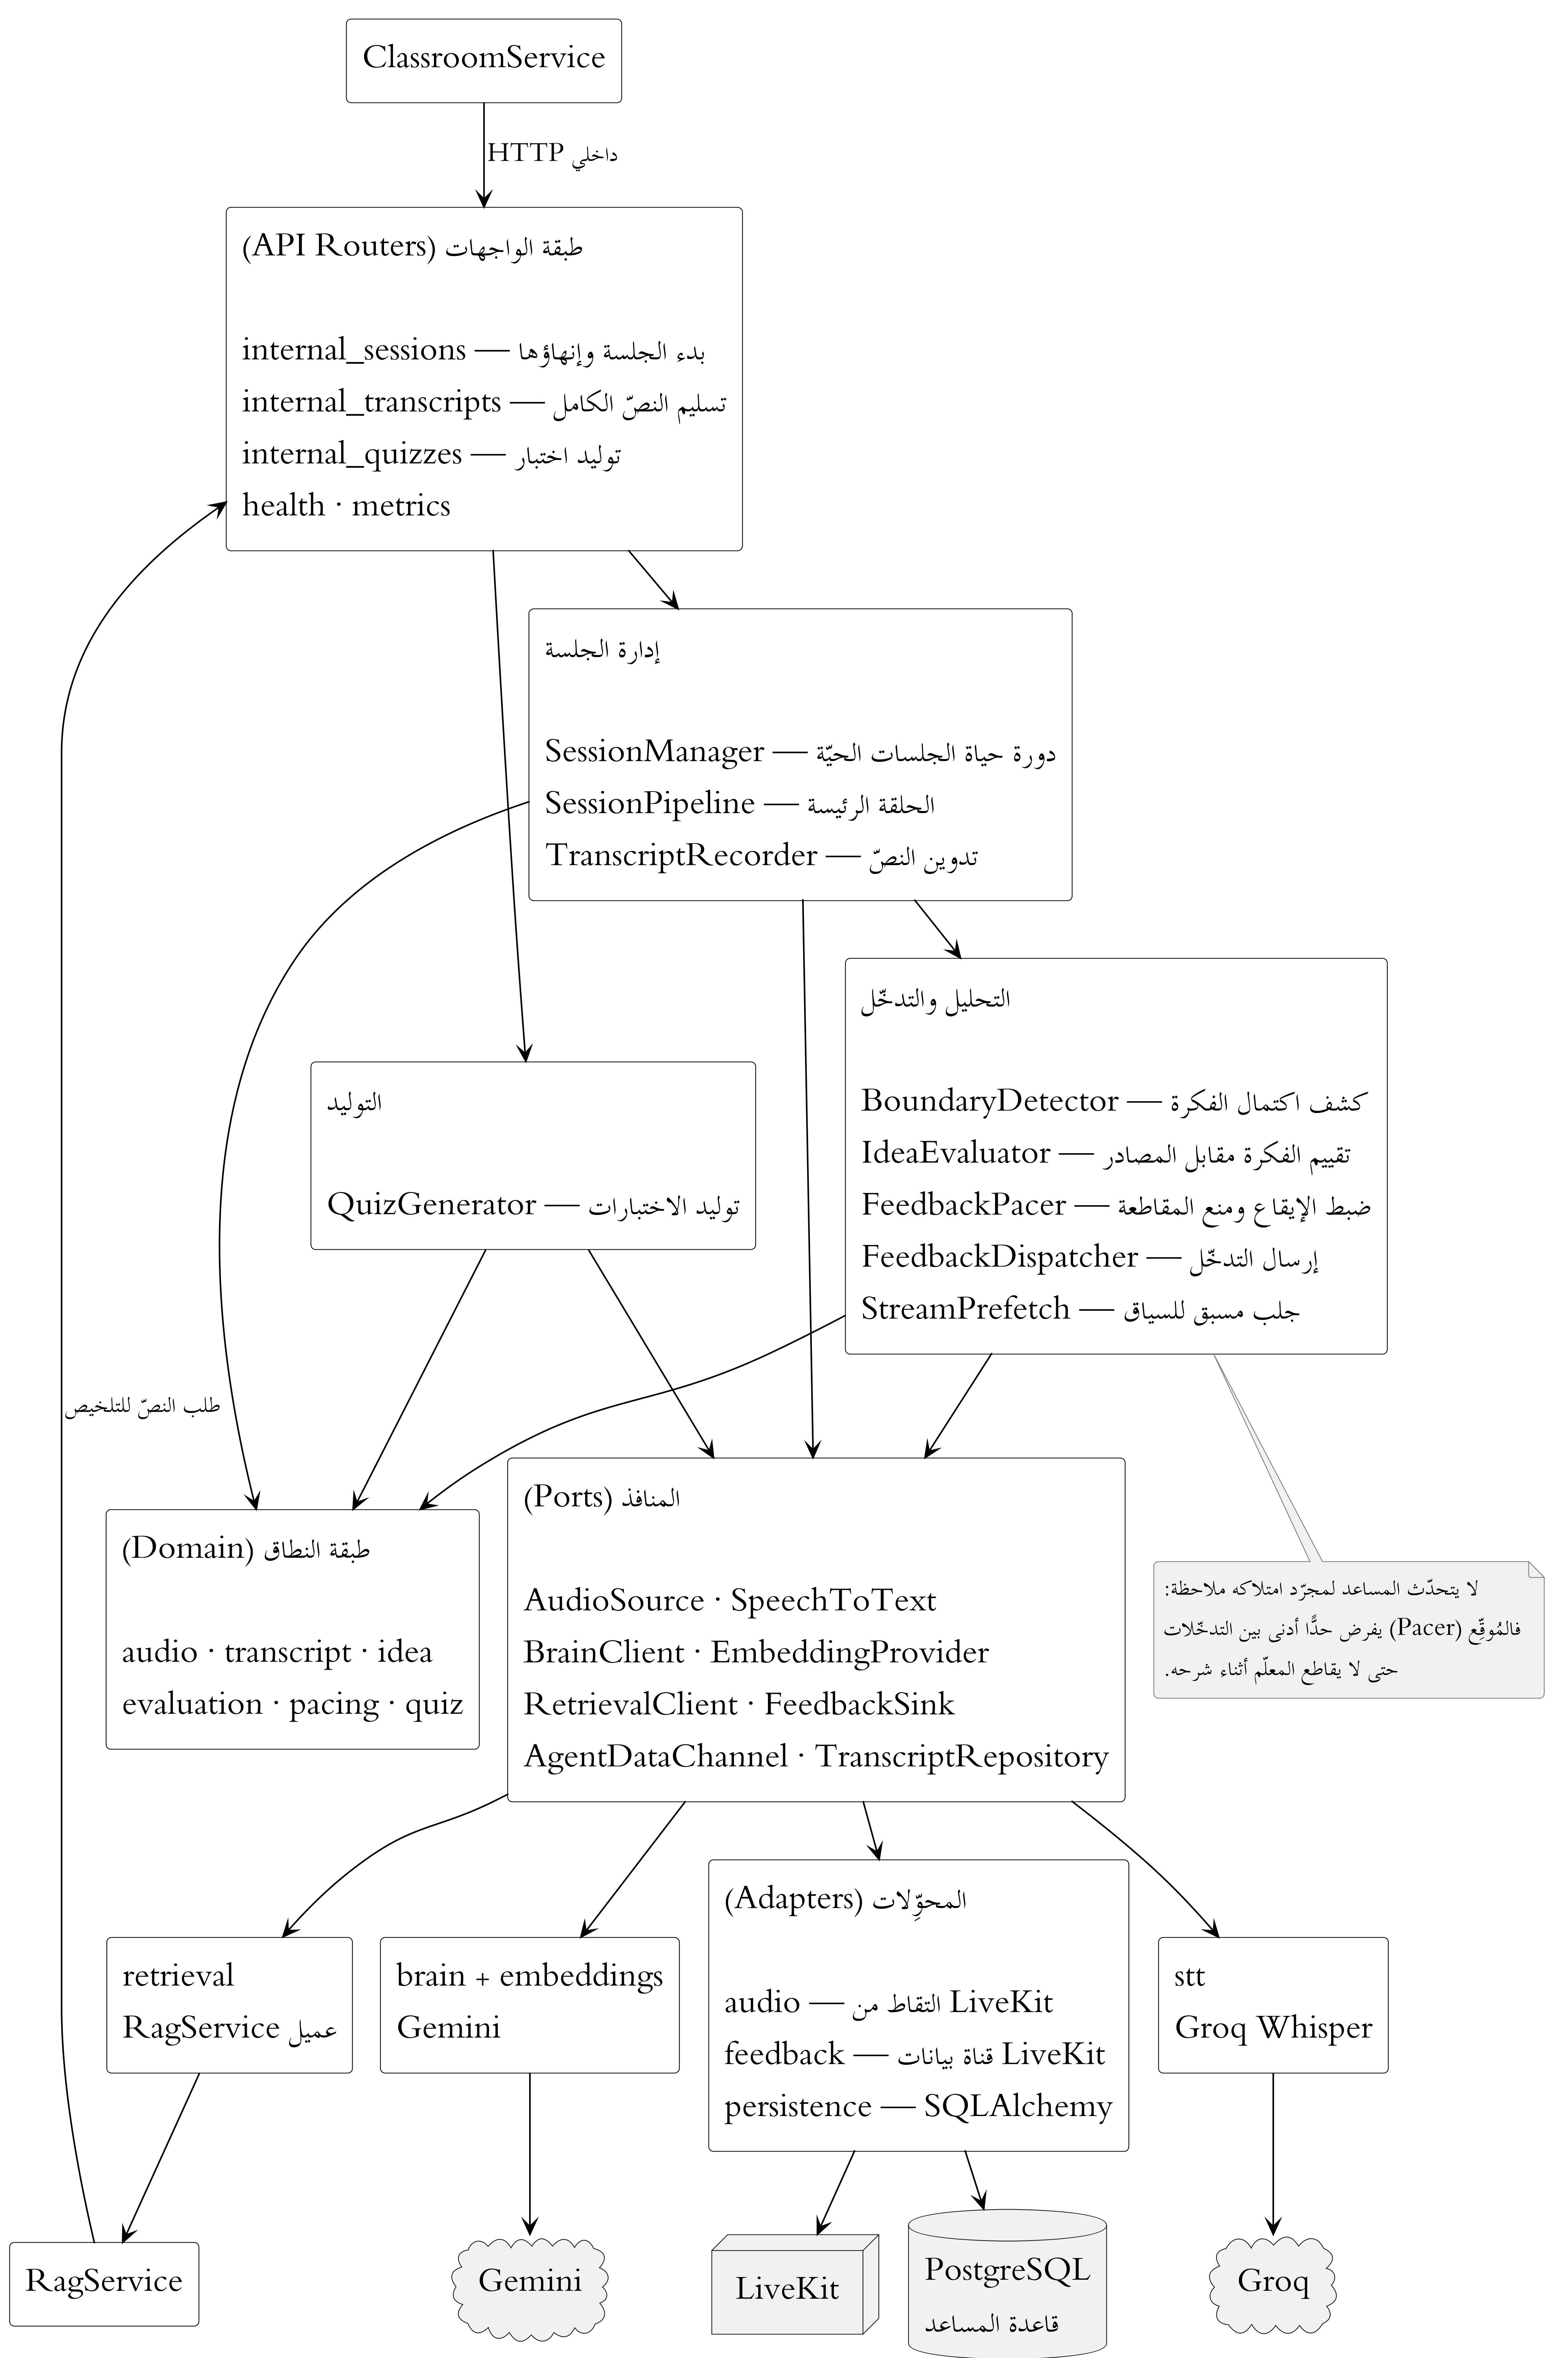
\includegraphics[width=\textwidth,height=0.8\textheight,keepaspectratio]{figures/comp-06-live-assistant.png}
  \caption{مخطط مكوّنات خدمة المساعد المباشر.}
  \label{fig:comp-06}
\end{figure}

وطُبّق في هذه الخدمة نمط المنافذ والمحوِّلات: يقابل كلَّ مورد خارجي منفذٌ مجرّد في طبقة التطبيق ومحوِّل واحد خلفه في طبقة البنية التحتية، وذلك لمصدر الصوت ومحرّك تحويل الكلام إلى نصّ والنموذج التوليدي ومزوّد التضمين وعميل الاسترجاع وقناة إرسال التدخّل ومستودع النصّ. ويتيح ذلك استبدال أيّ مزوّد دون تعديل منطق الحلقة، وتشغيل الحلقة كاملةً في الاختبارات بمحوِّلات بديلة لا تتّصل بشبكة.

وتحمل طبقة النطاق أنواع القرار نفسها: اكتمال الفكرة، ونتيجة التقييم ودرجة خطورتها، وقرار الإيقاع وسبب الكبح. وهي منطق خالص لا يستدعي نموذجًا ولا اتصالًا شبكيًّا ولا قاعدة بيانات، فتقبل الاختبار الوحدوي دون أيّ اعتماد خارجي.

ويفصل مُوقِّع التدخّل (\en{FeedbackPacer}) بين صحّة الملاحظة ووصولها إلى المعلّم، فيطبّق أربع قواعد بالترتيب، وتوقف أُولاها تحقّقًا الإرسالَ: حدّ أدنى لدرجة الثقة، وسقف لعدد التدخّلات في الجلسة الواحدة، وحدّ أدنى زمني بين تدخّلين متتاليين، ورفض الملاحظة المشابهة لما أُرسل ضمن نافذة زمنية محدّدة. والغرض منع مقاطعة المعلّم في أثناء الشرح.

وتُعرض الحلقة كاملةً، من التقاط الصوت إلى قرار التدخّل، في القسم~\ref{subsubsec:flow-live-loop}.

\subsection{نموذج البيانات}

لا تحفظ هذه الخدمة إلّا نصّ الجلسة؛ أمّا التسجيل والملخّص فيقعان في خدمة الفصول الدراسية ومخزن الملفّات. ويقوم النموذج على كيانين يعرضهما الشكل~\ref{fig:erd-05}: ترويسة النصّ (\en{session\_transcripts}) ومقاطعه المرتّبة زمنيًّا (\en{transcript\_segments}).

% [H]: pinned under the paragraph that introduces it. At 2.63:1 full width is
% only ~26% of the text block, so it fits without shrinking.
\begin{figure}[H]
  \centering
  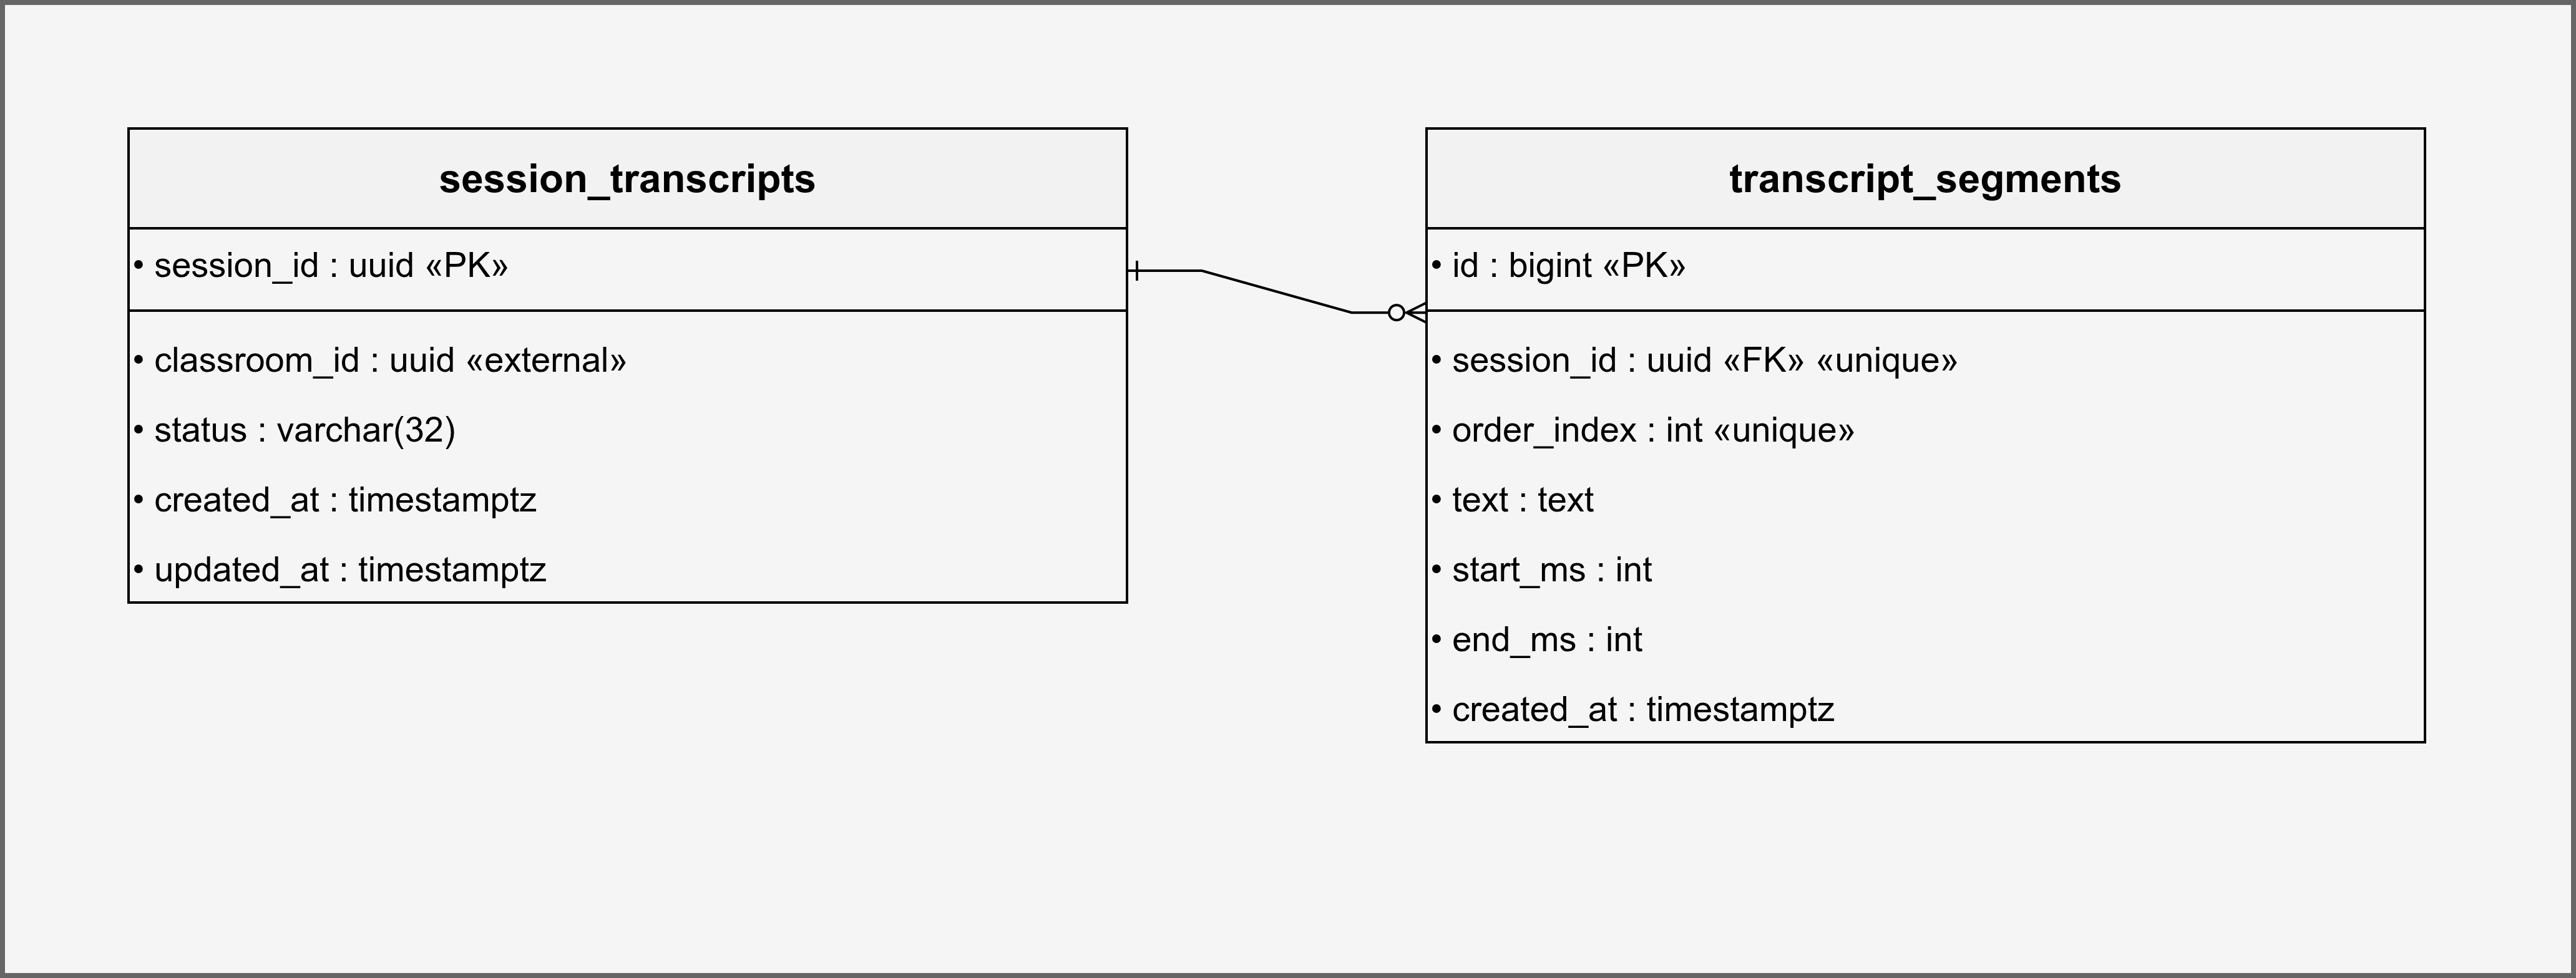
\includegraphics[width=\textwidth,height=0.8\textheight,keepaspectratio]{figures/erd-05-live-assistant.png}
  \caption{مخطط الكيانات والعلاقات لخدمة المساعد المباشر.}
  \label{fig:erd-05}
\end{figure}

ويضبط قيدُ فرادة مركّب على الزوج (\en{session\_id}, \en{order\_index}) تسلسلَ المقاطع داخل الجلسة ويمنع تكرار الرقم نفسه، في حين يؤدّي حذف الترويسة إلى حذف مقاطعها تتابعيًّا.


\chapter{بيئة التطوير والتقنيات المستخدمة}

% NOT YET WRITTEN in the Word draft — heading only.
% This chapter covers the concrete stack and the engineering results: the
% technologies chosen and why, the deployment setup, testing, and measured
% outcomes.

\begin{chaptersummary}
[ملخص الفصل.]
\end{chaptersummary}

\section{مقدمة}
[مقدمة الفصل.]

\section{التقنيات المستخدمة}
[لغات وأطر العمل المستخدمة في الواجهة الأمامية والخلفية.]

\section{بيئة النشر}
[الحاويات وتنسيقها، وإعداد بيئة التشغيل.]

\section{الاختبار والنتائج}
[الاختبارات الآلية والنتائج المقاسة.]

\section{الخاتمة}
[خاتمة الفصل.]


% ===========================================================================
% BACK MATTER
% ===========================================================================
\centredtitle{الخاتمة}
[الخاتمة: تلخص الهدف وما تم تحقيقه والنتائج، ثم الصعوبات التي واجهت العمل،
وتنتهي بالآفاق المستقبلية لتطويره.]
\clearpage

\centredtitle{المراجع}
\begin{english}
\begin{enumerate}
  \item Martin, R. C. (2017). \textit{Clean Architecture: A Craftsman's Guide to
        Software Structure and Design}. Prentice Hall.
  \item Newman, S. (2021). \textit{Building Microservices: Designing Fine-Grained
        Systems}. O'Reilly Media.
\end{enumerate}
\end{english}

\end{document}
